%
% Copyright (c) 2008  Betti Oesterholz
%
% Permission is granted to copy, distribute and/or modify this document
% under the terms of the GNU Free Documentation License, Version 1.2 or
% any later version published by the Free Software Foundation;
% with no Invariant Sections, no Front-Cover Texts, and no Back-Cover Texts.
%
% A copy of the license is included in the file ``fdl.tex'' .
%

%path for pictures
\graphicspath{{./klassendiagramme/}}
\graphicspath{{./klassendiagramme/}{../klassendiagramme}}


\newpage
\part{Implementation Fib-Sprachelemente}
\label{partImplementationFib}

In diesem Teil wird der Implementationsentwurf einer Bibliothek f"ur die Fib-Sprach\-ele\-mente vorgestellt. Dazu geh"ort die Klassenhierarchien und die Schnittstellenbeschreibungen. Die Schnittstellenbeschreibungen geschieht in pseudo C++.

Alle Fib-Element und Fib-Vektoren werden einem Namensraum mit dem Namen ``fib'' zugeordnet.

Alle Methoden sollten nach M"oglichkeit so definiert werden, dass es unm"oglich ist, ein ung"ultiges Fib-Objekt zu erzeugen. Das macht den Umgang mit den Methoden sicherlich schwieriger, aber auch sicherer.


\section{Hilfsmethoden}

Hilfsmethoden die bei der Implementierung Hilfreich sind, aber nicht zur eigentlichen Schnittstelle geh"oren, werden nach Bedarf implentiert, hier aber nicht aufgef"uhrt. Sie sollten nach M"oglichkeit von Au"sen nicht zugreifbar sein (also z. B. \verb|privat| oder \verb|protected| deklariert sein).


\section{Copyright}

Alle Fib-Sprachelemente werden unter die LGPL (siehe Abschnitt \ref{secLGPL} auf Seite \pageref{secLGPL}) gestellt. Auf diese Weise k"onnen sie als Bibliothek in beliebige andere Applikationen eingebunden werden.

Dies ist besonders f"ur Anzeigeprogramme/Abspielprogramme wichtig, da so die Copyright des Programms unabh"angig von der Fib-Bibliothek ist.


\section{Konstanten}

Im Fib-Namensraum werden ein paar Konstanten definiert:
\begin{itemize}
 \item \verb|FIB_VERSION|: Version der Multimediabeschreibungssprache Fib. Es handelt sich hier um eine positive ganze Zahl.
 \item \verb|FIB_DB_VERSION|: Version der Datenbank der Multimediabeschreibungssprache Fib. Es handelt sich hier um eine positive ganze Zahl.
 \item \verb|FIB_VERSION_NAME|: Name der Version der Multimediabeschreibungssprache Fib. Es handelt sich um eine Zeichenkette der Form ``Fib V1.0.2'' .
 \item \verb|FIB_DB_VERSION_NAME|: Name der Version der Datenbank der Multimediabeschreibungssprache Fib. Es handelt sich hier um eine Zeichenkette der Form ``Fib DB V2.3.1''
\end{itemize}


\section{Einfache Datentypen f"ur Zahlen}

Als primitive Datentypen f"ur Zahlen werden Fib eigene Namen benutzt, um eine einfache Erweiterbarkeit (z. B. Ausweitung des Definitionsbereichs) zu gew"ahrleisten.

\bigskip\noindent
Diese Datentypen sind:
\begin{itemize}
 \item \verb|intFib|: Ganzzahlen
 \item \verb|longFib|: nat"urliche Zahlen
 \item \verb|unsignedIntFib|: gro"se Ganzzahlen
 \item \verb|unsignedLongFib|: gro"se nat"urliche Zahlen
 \item \verb|doubleFib|: rationale Zahlen
\end{itemize}
Der Namensteil ``int'' deutet auf kleine Ganzzahlen hin und ``long'' auf gro"se. Der ``double'' Namensanfang steht f"ur Gleitkommazahlen. Beinhaltet der Name ``unsigned'' sind die Zahlen vorzeichenlos, bzw. nur positiv.

\bigskip\noindent
M"ogliche Entsprechungen in C++ k"onnten sein:
\begin{itemize}
 \item intFib: int
 \item longFib: long long
 \item doubleFib: double
 \item unsignedIntFib: unsigned int
 \item unsignedLongFib: unsigned long long
\end{itemize}


\section{Klassen f"ur Fib-Elemente}\index{Fib-Elemente}\index{Klassen!Fib-Elemente}

Sie Klasse \verb|cFibElement| ist die Basisklasse aller Fib-Elementklassen.

\bigskip\noindent
Es gibt folgende Fib-Elementklassen:
\begin{itemize}
 \item \verb|cPoint|: f"ur Punktelemente (siehe Abschnitt \ref{fibPoint} auf Seite \pageref{fibPoint})
 \item \verb|cProperty|: f"ur Eigenschaftselemente (siehe Abschnitt \ref{fibProperty} auf Seite \pageref{fibProperty})
 \item \verb|cList|: eine Liste von Fib-Objekten bzw. das Listenelement (siehe Abschnitt \ref{fibList} auf Seite \pageref{fibList})
 \item \verb|cComment|: f"ur Anmerkungselemente (siehe Abschnitt \ref{fibComment} auf Seite \pageref{fibComment})
 \item \verb|cArea|: f"ur Bereichselement (siehe Abschnitt \ref{fibArea} auf Seite \pageref{fibArea})
 \item \verb|cFunction|: f"ur Funktionselement (siehe Abschnitt \ref{fibFunction} auf Seite \pageref{fibFunction})
 \item \verb|cIf|: f"ur if-Bedingungselemente (siehe Abschnitt \ref{secFibIf} auf Seite \pageref{secFibIf})
 \item \verb|cExtObject|: f"ur externe Objekte (siehe Abschnitt \ref{fibExtObject} auf Seite \pageref{fibExtObject})
 \item \verb|cExtSubobject|: f"ur externe Unterobjekte (siehe Abschnitt \ref{fibSubobject} auf Seite \pageref{fibSubobject})
 \item \verb|cRoot|: f"ur Wurzelelemente (siehe Abschnitt \ref{fibRootElement} auf Seite \pageref{fibRootElement})
\end{itemize}
Die Fib-Elementklassen werden Klassen untergeordnet, welche ihre Struktur beschreiben:
\begin{itemize}
 \item \verb|cFibLeaf|: f"ur Fib-Elementklassen die Bl"atter sind, also keine Unterobjekte enthalten; die abgeleitete Klassen sind:
 \begin{itemize}
  \item \verb|cPoint|
  \item \verb|cExtSubobject|
 \end{itemize}
 \item \verb|cFibLimb|: f"ur Fib-Elementklassen die (gerade) Zweige sind, also genau ein Unterobjekt enthalten; die abgeleitete Klassen sind:
 \begin{itemize}
  \item \verb|cProperty|
  \item \verb|cList|
  \item \verb|cComment|
  \item \verb|cArea|
  \item \verb|cFunction|
 \end{itemize}
 \item \verb|cFibBranch|: f"ur Fib-Elementklassen die Verzweigungen darstellen, also mehrere Unterobjekte haben k"onnen; die abgeleitete Klassen sind:
 \begin{itemize}
  \item \verb|cList|
  \item \verb|cIf|
  \item \verb|cRoot|
  \item \verb|cExtObject|
 \end{itemize}
\end{itemize}

\subsection{Klassenhierarchie}\index{Fib-Elemente!Klassenhierarchie}

\begin{figure}[htbp]
\begin{center}
  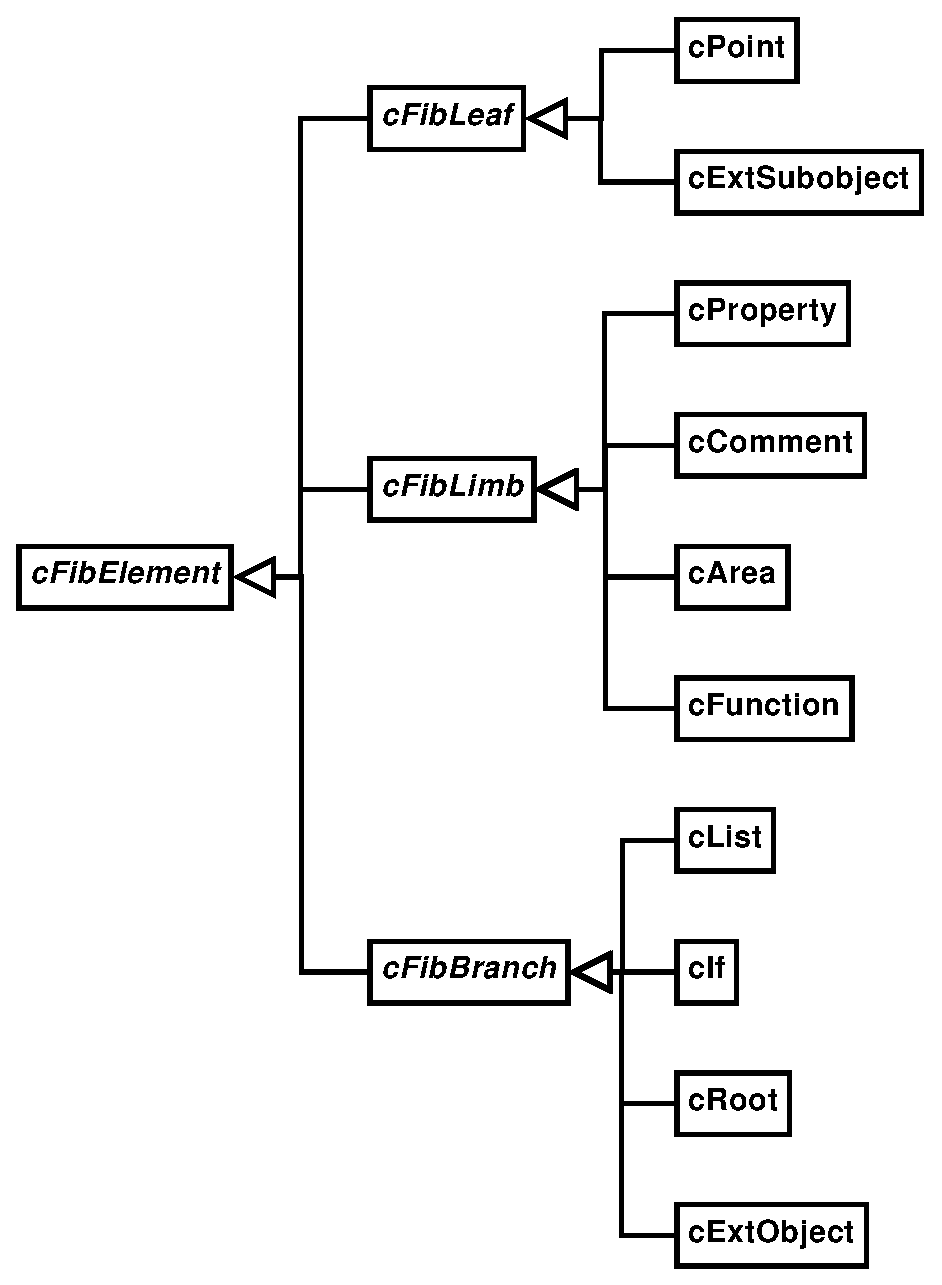
\includegraphics[scale=0.4]{fib_elemente}
\end{center}
\caption{Klassengraph Fib-Elemente}
\label{figClassFibElements}
\end{figure}

In Abbildung \ref{figClassFibElements} ist die Vererbungsstruktur der Klassen f"ur Fib-Elemente zu sehen. Wie zu sehen werden alle Fib-Elementklassen von der Klasse \verb|cFibElement| abgeleitet.


\section{Fib-Elemente Klasse cFibElement}\index{Fib-Elemente}\index{cFibElement}\index{Klassen!cFibElement}

Die Klasse \verb|cFibElement| ist die Basisklasse aller Fib-Element. Sie ist eine abstrakte Klasse, von ihr selbst k"onnen keine Objekte erzeugt werden.

\subsection{Schnittstellenbeschreibung}

Im Nachfolgenden werden die Methoden und Funktionen beschrieben, welche von allen Fib-Elementen bereitgestellt und von der Klasse \verb|cFibElement| deklariert werden. Diese Methoden und Funktionen dienen haupts"achlich dazu, die Struktur eines Fib-Objektbaums zu analysieren und anzupassen.

Externe Unterobjekte werden nur von Methoden aufgel"ost, bei denen es explizit erw"ahnt wird.

Alle Zahlen mit denen Fib-Elemente oder Objekte identifiziert werden (siehe Abschnitte "uber die Ordnung der Fib-Elemente ab Seite \pageref{secOrderFibElements}), werden bez"uglich des Fib-Elements angegeben, bei dem die entsprechende Methode aufgerufen wird, und nicht dem obersten root-Element. Soll beispielsweise das dritte Punktelement zur"uckgegeben werden, wird das dritte Punktelement bez"uglich des Fib-Elements zur"uckgegeben, an dem die entsprechende Methode aufgerufen wurde, und nicht bez"uglich des obersten root-Elements, f"ur welches dieses dritte Punktelement bez"uglich des Fib-Elements das neunte Punktelement sein k"onnte.
Dies gilt nat"urlich nur, wenn nicht explizit ein anderer Bezugspunkt angegeben wird.

\subsubsection{Typ edDirection}\index{edDirection}
\label{secEdDirection}

Der Typ \verb|edDirection| dient zur Angabe einer Richtung im Fib-Objekt. Diese Angabe sollte zu einem Referenz-Fib-Element im Fib-Objekt geschehen. (Zur Definition von ``Oben'' und ``Unten'' siehe Abschnitt \ref{secDefinitionUpDown} auf Seite \pageref{secDefinitionUpDown} .)

\bigskip\noindent
G"ultige Werte sind:
\begin{itemize}
 \item \verb|ED_ALL|: in alle Richtungen im Fib-Objekt vom Referenz-Fib-Element ausgehend
 \item \verb|ED_POSITION|: das Referenz-Fib-Element
 \item \verb|ED_BELOW|: alle Fib-Elemente unter dem Referenz-Fib-Element
 \item \verb|ED_HIGHER|: alle Fib-Elemente "uber dem Referenz-Fib-Element
 \item \verb|ED_BELOW_EQUAL|: alle Fib-Elemente unter dem Referenz-Fib-Element und das Referenz-Fib-Element
 \item \verb|ED_HIGHER_EQUAL|: alle Fib-Elemente "uber dem Referenz-Fib-Element und das Referenz-Fib-Element
\end{itemize}


\subsubsection{getType}\index{cFibElement!getType()}\index{getType()}
\label{secGetType}

\textbf{Syntax:} \verb|char getType() const|

\bigskip\noindent
"Uber die Methode kann der Typ des Objekts bzw. des Fib-Elements ermittelt werden.

\bigskip\noindent
\textbf{M"ogliche Typen sind:}
\begin{itemize}
 \item['u':] (=117) unbekannten Type; als Parameter einer Methode steht dieser Wert f"ur Fib-Elemente aller Typen
 \item['p':] (=112) f"ur Punkt-Elemente (cPoint)
 \item['y':] (=121) f"ur Eigenschaftselemente (cProperty)
 \item['l':] (=108) f"ur Listenelemente (cListen)
 \item['c':] (=110) f"ur Anmerkungselemente (cComment)
 \item['a':] (=97) f"ur Bereichselemente (cArea)
 \item['f':] (=102) f"ur Funktionselemente (cFunction)
 \item['i':] (=105) f"ur if-Bedingungen (cIf)
 \item['o':] (=111) f"ur externe Objekte (cExtObject)
 \item['s':] (=115) f"ur externe Unterobjekte (cExtSubobject)
 \item['v':] (=118) f"ur set-Elemente (cFibSet)
 \item['m':] (=109) f"ur Matrixelement (cFibMatrix)
 \item['r':] (=114) f"ur Wurzelelemente (cRoot)
\end{itemize}

\noindent
\textbf{Eingabeparameter:} keine

\bigskip\noindent
\textbf{R"uckgabe:} Es wird eine Konstante zum Identifizieren des Objekts zur"uckgegeben.


\subsubsection{getTypeName}\index{cFibElement!getTypeName()}\index{getTypeName()}

\textbf{Syntax:} \verb|static string getTypeName( char cType ) const|

\bigskip\noindent
Diese Methode wandelt das Typezeichen eines Fib-Elements in dessen Bezeichnung um.

\bigskip\noindent
\textbf{Eingabeparameter:}
\begin{itemize}
 \item \verb|cType:| Das Typzeichen, welches umzuwandeln ist.
\end{itemize}
\textbf{R"uckgabe:} Der Text f"ur die Elementbezeichnung f"ur den eingegeben Typen:

\begin{center}
\begin{tabular}{|p{20mm}|p{30mm}|}\hline
	Typ\-zeichen & Elementbezeichnung \\\hline\hline
	'u' & ``unknown''\\\hline
	'p' & ``point''\\\hline
	'y' & ``property''\\\hline
	'l' & ``list''\\\hline
	'm' & ``comment''\\\hline
	'a' & ``area''\\\hline
	'f' & ``function''\\\hline
	'i' & ``if''\\\hline
	'o' & ``extern object''\\\hline
	's' & ``extern subobject''\\\hline
	'r' & ``root''\\\hline
\end{tabular}
\end{center}

\subsubsection{getSuperiorFibElement}\index{cFibElement!getSuperiorFibElement()}\index{getSuperiorFibElement()}

\textbf{Syntax:} \verb|cFibElement* getSuperiorFibElement()|

\bigskip\noindent
Die Methode holt das n"achste Fib-Element im Fib-Baum, welches dieses Fib-Element enth"alt. Wenn kein solches Fib-Element existiert, wird ein Nullpointer \verb|NULL| zur"uckgegeben.

\bigskip\noindent
\textbf{Eingabeparameter:} keine

\bigskip\noindent
\textbf{R"uckgabe:} Einen Zeiger auf das n"achste Fib-Element, welches dieses Fib-Element enth"alt, oder der Nullpointer \verb|NULL|, wenn kein solches Fib-Element existiert.


\subsubsection{getNextFibElement}\index{cFibElement!getNextFibElement()}\index{getNextFibElement()}
\textbf{Syntax:} \verb|cFibElement* getNextFibElement()|

\bigskip\noindent
Die Methode holt das n"achste Fib-Element im Fib-Baum. Wenn kein solches Fib-Element existiert, wird ein Nullpointer \verb|NULL| zur"uckgegeben. Die Reihenfolge bezieht sich auf die Ordnung der Fib-Elemente.

\bigskip\noindent
\textbf{Eingabeparameter:} keine

\bigskip\noindent
\textbf{R"uckgabe:} Einen Zeiger auf das n"achste Fib-Element oder der Nullpointer \verb|NULL|, wenn kein solches Fib-Element existiert.


\subsubsection{getNextFibElement}\index{cFibElement!getNextFibElement()}\index{getNextFibElement()}

\textbf{Syntax:} \verb|cFibElement* getNextFibElement( char cType )|

\bigskip\noindent
Die Methode holt das n"achste Fib-Element im Fib-Baum vom angegeben Typ. Wenn kein solches Fib-Element existiert, wird ein Nullpointer \verb|NULL| zur"uckgegeben. Die Reihenfolge bezieht sich auf die Ordnung der Fib-Elemente.

\bigskip\noindent
\textbf{Eingabeparameter:}
\begin{itemize}
 \item \verb|cType|: Der Typ des Fib-Elements, welches zur"uckgegeben werden soll. Der Typ 'w' steht f"ur das n"achste Falsche (=``wrong'') Fib-Element, also ein Fib-Element, welches noch nicht korrekt mit Parametern beladen ist (es fehlt beispielsweise ein Unterobjekt).
\end{itemize}

\bigskip\noindent
\textbf{R"uckgabe:} Einen Zeiger auf das n"achste Fib-Element mit dem angegeben Typ oder der Nullpointer \verb|NULL|, wenn kein solches Fib-Element existiert.


\subsubsection{getFibElement}\index{cFibElement!getFibElement()}\index{getFibElement()}

\textbf{Syntax:} \verb|cFibElement* getFibElement( longFib lNumber,| \\\verb| bool bAbsolute=false )|

\bigskip\noindent
Die Methode holt das \verb|lNumber|'te Fib-Element. Wenn kein solches Fib-Element existiert, wird ein Nullpointer \verb|NULL| zur"uckgegeben.

\bigskip\noindent
\textbf{Eingabeparameter:}
\begin{itemize}
 \item \verb|lNumber|: Die Nummer, die das zu holende Fib-Element im aktuellen Fib-Baum/Objekt hat.
 \item \verb|bAbsolute|: Wenn \verb|bAbsolute| gleich \verb|true| ist, bezieht sich die \verb|lNumber| auf das gesamte Fib-Objekt. Ansonsten, wenn \verb|bAbsolute| gleich \verb|false| ist, bezieht sich \verb|lNumber| auf das Fib-Element von dem aus die Methode aufgerufen wurde. Standardwert ist \verb|false|.
\end{itemize}

\bigskip\noindent
\textbf{R"uckgabe:} Einen Zeiger auf das Fib-Element, vom Typ des aktuellen Fib-Elements, welches an der angegebene Position \verb|lNumber| steht oder der Nullpointer \verb|NULL|, wenn kein solches Fib-Element existiert.


\subsubsection{getFibElement}\index{cFibElement!getFibElement()}\index{getFibElement()}

\textbf{Syntax:} \verb|cFibElement* getFibElement(| \\\verb| char cType, longFib lNumber,| \\\verb| bool bAbsolute=false )|

\bigskip\noindent
Die Methode holt das \verb|lNumber|'te Fib-Element von dem angegebenen Typ \verb|cType|. Wenn kein solches Fib-Element existiert, wird ein Nullpointer \verb|NULL| zur"uckgegeben.

\bigskip\noindent
\textbf{Eingabeparameter:}
\begin{itemize}
 \item \verb|cType|: Der Typ des Fib-Elements, welches zur"uck geliefert werden soll. Der Typ 'w' steht f"ur das n"achste Falsche (=``wrong'') Fib-Element, also ein Fib-Element, welches noch nicht korrekt mit Parametern beladen ist (es fehlt beispielsweise ein Unterobjekt).
 \item \verb|lNumber|: Die Nummer, die das zu holende Fib-Element im aktuellen Fib-Baum/Objekt hat.
 \item \verb|bAbsolute|: Wenn \verb|bAbsolute| gleich \verb|true| ist, bezieht sich die \verb|lNumber| auf das gesamte Fib-Objekt. Ansonsten, wenn \verb|bAbsolute| gleich \verb|false| ist, bezieht sich \verb|lNumber| auf das Fib-Element von dem aus die Methode aufgerufen wurde. Standardwert ist \verb|false|.
\end{itemize}

\bigskip\noindent
\textbf{R"uckgabe:} Einen Zeiger auf das Fib-Element, vom angegeben Typ \verb|cType|, welches an der angegebene Position \verb|lNumber| steht oder der Nullpointer \verb|NULL|, wenn kein solches Fib-Element existiert.


\subsubsection{getAllFibElements}\index{cFibElement!getAllFibElements()}\index{getAllFibElements()}

\textbf{Syntax:} \verb|list<cFibElement*> getAllFibElements(| \\\verb| char cTypeBasis='u',| \\\verb| longFib lNumber=0, char cType='u',| \\\verb| edDirection direction=ED_ALL , unsignedLongFib| \\\verb| lNumberOfMaxReturnedElements=0 | \\\verb| bool bAbsolute=false )|

\bigskip\noindent
Die Methode gibt eine Liste mit den Zeigern zu den Fib-Elemente vom angegebenen Typ \verb|cType| zur"uck, welche sich in der Richtung \verb|direction| (siehe \ref{secEdDirection} Seite \pageref{secEdDirection}) vom \verb|lNumber|'te Objekt vom angegeben Typ \verb|cTypBasis| befinden.

Dabei werden  niemals mehr als \verb|lNumberOfMaxReturnedElements| Fib-Element zur"uckgegeben, wobei der Wert $0$ bei \verb|lNumberOfMaxReturnedElements| f"ur unendlich steht. Alle zur"uckgegebenen Fib-Elemente stammen aus dem Ast, in dem sich auch das Referenz-Fib-Element befindet.

Wenn von mehreren Richtungen oder/und Unterobjekten Fib-Elemente zur"uckzugeben sind, wird versucht von jeder Richtung oder/und Unterobjekt die gleiche Anzahl Fib-Elemente zur"uckzugeben.

\bigskip\noindent
\textbf{Eingabeparameter:}
\begin{itemize}
 \item \verb|cTypeBasis|: Der Typ, welchen das Referenz-Fib-Element im aktuellen Fib-Baum/Objekt hat. Standardwert ist 'u', womit Fib-Elemente aller Typen (bzw. keines bestimmten Typs) betrachtet werden.
 \item \verb|lNumber|: Die Nummer, welches das Referenz-Fib-Element im aktuellen Fib-Baum/Objekt hat. Standardwert ist $0$, womit alle Fib-Elemente vom aktuellen Fib-Element ausgehend zur"uckgeliefert werden, unabh"angig vom angegeben Typ \verb|cTypeBasis|.
 \item \verb|cType|: Der Typ der Fib-Elemente, welche zur"uck geliefert werden soll. Standardwert ist 'u', womit Fib-Elemente aller Typen (bzw. keines bestimmten Typs) zur"uckgegeben werden. Der Typ 'w' steht f"ur Falsche (=``wrong'') Fib-Elemente, also Fib-Elemente, welche noch nicht korrekt mit Parametern beladen sind (es fehlt beispielsweise ein Unterobjekt).
 \item \verb|direction|: Die Richtung vom Referenz-Fib-Element ausgehend, von der alle Fib-Elemente mit dem angegeben Typ zur"uckzugeben sind. Standardwert ist hierf"ur \verb|ED_ALL|, so dass Fib-Elemente aus dem gesamten Ast des Referenz-Fib-Elements zur"uckgegeben werden.
 \item \verb|lNumberOfMaxReturnedElements|: Die Anzahl der maximal zur"uckzugebenden Fib-Elemente. Ist der Wert $0$, gibt es keine Begrenzung f"ur die Anzahl der zur"uckzugebenden Fib-Elemente. Standardwert ist $0$ (=unbegrenzt).
 \item \verb|bAbsolute|: Wenn \verb|bAbsolute| gleich \verb|true| ist, bezieht sich die \verb|lNumber| auf das gesamte Fib-Objekt. Ansonsten, wenn \verb|bAbsolute| gleich \verb|false| ist, bezieht sich \verb|lNumber| auf das Fib-Element von dem aus die Methode aufgerufen wurde. Standardwert ist \verb|false|.
\end{itemize}

\bigskip\noindent
\textbf{R"uckgabe:} Eine Liste mit den entsprechenden Fib-Elementen.


\subsubsection{evalueObject}\index{cFibElement!evalueObject()}\index{evalueObject()}
\label{secEvalueObjectPosition}

\textbf{Syntax:} \verb|bool evalueObject(| \\\verb| iEvaluePosition & evaluePosition,| \\\verb| const unsignedIntFib objectPoint=0,| \\\verb| list<cVectorProperty> &liVecProperties=| \\\verb| list<cVectorProperty>() ) const|

\bigskip\noindent
"Uber die Methode \verb|evalueObject| k"onnen Fib-Objekte ausgewertet werden.

Der Methode wird eine Referenz auf ein Object (\verb|evaluePosition|) vom Type \verb|iEvaluePosition| "ubergeben, "uber welche die einzelnen Punkt mit ihren Eigenschaften ausgewertet werden. Jedes mal, wenn ein Punkt dargestellt/ ausgewertet werden soll, wird die Methode \verb|evaluePosition()| des Objects mit der Position des Punktes und einer Liste seiner Eigenschaften aufgerufen. Auf diese Weise kann die Methode \verb|evalueObject| f"ur verschiedene Aufgaben genutzt werden. Soll ein Objekt als Bild ausgewertet werden, stellt die Methode \verb|evaluePosition()| einen Punkt im Bild dar. Wenn das Objekt mit einem anderen Multimediaobjekt verglichen werden soll, vergleicht die Methode \verb|evaluePosition()| die einzelnen Punkte (Vorsicht ist geboten, wenn ein Punkt einen anderen "uberdeckt). Die Methode \verb|evaluePosition()| muss nur entsprechend implementiert werden.
Gibt ein Aufruf der Methode \verb|evaluePosition()| false zur"uck, wird die Auswertung des Fib-Objekts mit \verb|evalueObject| abgebrochen.
N"aheres zu Objekten, welche das Interface \verb|iEvaluePosition| implementieren im Abschnitt \ref{secIEvaluePosition} auf Seite \pageref{secIEvaluePosition} .

Von der Methode \verb|evalueObject| werden auch externe Objekte aufgel"ost. Auf diese Weise wird das komplette Multimediaobjekt ausgewertet, welches des Fib-Objekt darstellt.

\bigskip\noindent
\textbf{Eingabeparameter:} 
\begin{itemize}
 \item \verb|evaluePosition|: Eine Referenz auf ein Object zum auswerten/ speichern der einzelnen Punkte mit ihren Eigenschaften. Dieses Object stellt die Methode \verb|evaluePosition()| bereit, der f"ur jeden Punkt, der ausgewertet werden soll, die Position und eine Liste mit Eigenschaften des Punktes "ubergeben wird.
 \item \verb|objectPoint|: Der Objektpunkt des echten Teilobjekts, welches ausgewertet werden soll. Standardm"a"sig wird dieser Wert auf $0$ gesetzt und damit das gesamt Objekt ausgewertet.
 \item \verb|liVecProperties|: Eine Liste mit den Eigenschaften, die das auszuwertende Objekt global besitzen soll. Diese Eigenschaften werden jeden Punkt zugeordnet, soweit sie nicht "uberschrieben werden. Standardm"a"sig wird hier eine leere Liste, also keine globalen Eigenschaften, "ubergeben.
\end{itemize}

\bigskip\noindent
\textbf{R"uckgabe:} Diese Methode gibt \verb|true| (=wahr) zur"uck, wenn die Auswertung des Objekts erfolgreich war, sonst \verb|false| (=falsch).


\subsubsection{evalueObject}\index{cFibElement!evalueObject()}\index{evalueObject()}
\label{secEvalueObjectFibElement}

\textbf{Syntax:} \verb|bool evalueObject(| \\\verb| iEvalueFibElement & evalueFibElement,| \\\verb| const unsignedIntFib objectPoint=0,| \\\verb| list<cVectorProperty> &liVecProperties=| \\\verb| list<cVectorProperty>(),| \\\verb| conat list<char> liCFibElementTyps )|


\bigskip\noindent
"Uber die Methode \verb|evalueObject| k"onnen Fib-Objekte ausgewertet werden.

Der Methode wird eine Referenz auf ein Object (\verb|evalueFibElement|) vom Type \verb|iEvalueFibElement| "ubergeben, "uber welche die einzelnen Fib-Elemente mit ihren Eigenschaften ausgewertet werden. Jedes mal, wenn ein Fib-Elemente dargestellt/ ausgewertet werden soll, wird die Methode \verb|evalueElement()| des Objects mit einem Zeiger auf des Fib-Elemente und einer Liste seinen Eigenschaften aufgerufen. Auf diese Weise kann die Methode \verb|evalueObject| f"ur verschiedene Aufgaben genutzt werden.
Gibt ein Aufruf der Methode \verb|evalueElement()| false zur"uck, wird die Auswertung des Fib-Objekts mit \verb|evalueObject| abgebrochen.
N"aheres zu Objekten, welche das Interface \verb|iEvalueFibElement| implementieren im Abschnitt \ref{secIEvalueFibElement} auf Seite \pageref{secIEvalueFibElement} .

"Uber die Liste \verb|liCFibElementTyps| wird bestimmt, welche Fib-Element zur"uckgegeben werden sollen. F"ur jedes Fib-Element das zur"uckgegeben werden soll, steht in \verb|liCFibElementTyps| sein Typzeichen (siehe Abschnitt \ref{secGetType} auf Seite \pageref{secGetType}). Punktelemente mit Positionsvektoren werden immer zur"uckgegeben. Diese m"u"sen nicht seperat in \verb|liCFibElementTyps| aufgef"uhrt werden.

\bigskip\noindent
\textbf{Eingabeparameter:} 
\begin{itemize}
 \item \verb|evalueFibElement|: Eine Referenz auf ein Object zum auswerten/ speichern der einzelnen Fib-Elemente mit ihren Eigenschaften. Dieses Object stellt die Methode \verb|evalueElement()| bereit, der f"ur jedes Fib-Element, mit einem Type aus der Liste \verb|liCFibElementTyps| oder das ein Punkt ist, ein Zeiger auf das Fib-Element und eine Liste mit Eigenschaften des Fib-Elements "ubergeben wird.
 \item \verb|objectPoint|: Der Objektpunkt des echten Teilobjekts, welches ausgewertet werden soll. Standardm"a"sig wird dieser Wert auf $0$ gesetzt und damit das gesamt Objekt ausgewertet.
 \item \verb|liVecProperties|: Eine Liste mit den Eigenschaften, die das auszuwertende Objekt global besitzen soll. Diese Eigenschaften werden jeden Blattelement zugeordnet, soweit sie nicht "uberschrieben werden. Standardm"a"sig wird hier eine leere Liste, also keine globalen Eigenschaften, "ubergeben.
 \item \verb|liCFibElementTyps|: Die Liste mit den Typzeichen f"ur die Fib-Element, f"ur die \verb|auf()| aufgerufen werden soll. Die m"oglichen Zeichen werden in Abschnitt \ref{secGetType} auf Seite \pageref{secGetType} aufgef"uhrt.
\end{itemize}

\bigskip\noindent
\textbf{R"uckgabe:} Diese Methode gibt \verb|true| (=wahr) zur"uck, wenn die Auswertung des Objekts erfolgreich war, sonst \verb|false| (=falsch).


\subsubsection{getTimeNeed}\index{cFibElement!getTimeNeed()}\index{getTimeNeed()}\index{Auswertungszeit}

\textbf{Syntax:} \verb|unsignedLongFib getTimeNeed( | \\\verb| unsignedLongFib lMaxTime=0 ) const|

\bigskip\noindent
Diese Methode berechnet einen Wert f"ur die Zeit, welche zur Auswertung des Fib-Objekts ben"otigt wird.

Von der Methode \verb|getTimeNeed| werden auch externe Objekte aufgel"ost und in der Berechnung ber"ucksichtigt.

Der Eingabeparameter \verb|lMaxTime| dient dazu, den Aufwand zum Berechnen der Zeit zu begrenzen. Wenn ein Fib-Objekt sehr Zeitaufw"andig auszuwerten ist, w"urde auch das Ermitteln der Zeitstatistik entsprechend lange dauern. Mit dem Parameter \verb|lMaxTime| wird die Zeit zur Berechnung der Zeitstatistik begrenzt bzw. abgebrochen, wenn \verb|lMaxTime| erreicht wurde. Wenn der Wert \verb|lMaxTime| nicht angegeben wird oder $0$ ist, wird die Berechnungszeit nicht begrenzt.

N"utzlich ist diese Begrenzung, da eine genetische Operation die Auswertungszeit sehr stark erh"ohen kann. Durch die Begrenzung kann die Zeit zum Ermitteln der Zeitstatistik begrenzt werden und alle Individuen, die diese Grenze erreichen sofort verworfen/ gel"oscht werden.

In Tabelle \ref{tabTimeNeed} sind die Formeln f"ur die ben"otigten Zeiten f"ur die einzellnen Elemente aufgef"uhrt. Dabei bezeichnet $T$ die Auswertungszeit eines Fib-Elements und $T(Obj_i)$ die Auswertungszeit des i'ten enthaltenden Fib-Objekts.

\begin{center}
\begin{longtable}{|p{22mm}|p{50mm}|p{50mm}|}\hline
	Fib-Ele\-ment\-klasse & Zeitformel & Anmerkung \\\hline\endhead

	\verb|cPoint|    & $T(Obj)= 1 + E_V$ & $E_V$ ist die Anzahl der Elemente des Positionsvektors \\\hline
	\verb|cProperty| & $T(Obj)= 1 + E_V + T(Obj_1)$ & $E_V$ ist die Anzahl der Elemente des Eigenschaftsvektor; $T(Obj_1)$ die Auswertungszeit des enthaltenden Fib-Objekts $Obj_1$\\\hline
	\verb|cList|  & $T(Obj)= 1 + \sum^{n}_{i=1} T(Obj_i)$ & $T(Obj_i)$ sind die Auswertungszeiten der enthaltenden Fib-Unterobjekte $Obj_i$; $n$ ist die Anzahl der enthaltenden Fib-Unterobjekte\\\hline
	\verb|cComment|: & $T(Obj)= 1 + T(Obj_1)$ & $T(Obj_1)$ ist die Auswertungszeit des enthaltenden Fib-Objekts $Obj_1$\\\hline
	\verb|cArea|: & $T(Obj)= 1 + \sum_{W \in B_1 \ldots B_n} T( Obj_1(W) )$ & $B_i$ sind die Unterbereiche des Bereichs, mit $n$ der Anzahl der Unterbereiche; $W$ sind dann die einzelnen Werte der Bereiche; $T( Obj_1(W) )$ ist die Auswertungszeit des enthaltenden Fib-Objekts $Obj_1$, wenn die Variable des Bereichselements auf $W$ gesetzt wurde \\\hline
	\verb|cFunction| & $T(Obj)= T(UF) + T( Obj_1(W) )$ & $T(UF)$ ist die Zeit, welche zu Berechnen der Unterfunktion ben"otigt wird;  $T( Obj_1(W) )$ ist die Auswertungszeit des enthaltenden Fib-Objekts $Obj_1$, wenn die Variable des Funktionselements auf $W$, den Wert der Funktion, gesetzt wurde \\\hline
	\verb|cIf|       & $T(Obj)= T(UB) + if ( UB==true )\{ T(Obj_1)\} else \{ T(Obj_2)\}$ & $T(UB)$ ist die Zeit, welche zu Berechnen der Unterbedingung ben"otigt wird; $T(Obj_1)$ und $T(Obj_2)$ die Auswertungszeiten der enthaltenden Fib-Objekte $Obj_1$ und $Obj_2$, es wird jeweils die Auswertungszeit desjenigen Objekts hinzuaddiert, welches bei der Unterbedingungsauswertung auch ausgewertet w"urde (als $Obj_1$ wenn die Unterbedingung wahr ist und sonst $Obj_2$)\\\hline
	\verb|cExtObject| & $T(Obj)= 5 + T(Obj_1)$ & $T(Obj_1)$ ist die Auswertungszeit des Fib-Objekts $Obj_1$, welches durch das externe Objekte repr"asentiert wird\\\hline
	\verb|cExtSub-| \verb|object| & $T(Obj)= 2 + T(Obj_1)$ & $T(Obj_1)$ ist die Auswertungszeit des Fib-Objekts $Obj_1$, welches hier jeweils eingesetzt bzw. extern bereitgestellt wird\\\hline
	\verb|cFibSet| & $T(Obj)= n * \sharp DefVar +$ $\sum_{V \in V_1 \ldots V_n} T( Obj_1(V) )$ & $\sharp DefVar$ ist die Anzahl der vom set-Element definierten Variablen;$V_i$ sind die Vektoren mit den zu setzenden Werten des set-Elements, mit $n$ der Anzahl der Vektoren; $V$ sind dann die einzelnen Vektoren; $T( Obj_1(V) )$ ist die Auswertungszeit des enthaltenden Fib-Objekts $Obj_1$, wenn die definierten Variable des set-Elements auf die entsprechenden Elementwerte von $V$ gesetzt wurden \\\hline
	\verb|cFibMatrix| & $T(Obj)= if ( i not 0 )\{$ $\sum_{V \in V_1 \ldots V_k}( d + i + T( Obj_1(D(V),V) ) )$ $\}else\{$ $\sum_{v_1 = Startvalue_1 \ldots Endvalue_1} \ldots$ $sum_{v_d = Startvalue_d \ldots Endvalue_d} ($ $d + T( Obj_1(v_1, \ldots, v_d ) ) ) \}$ &  Die Zeitbereichnung von Matrixelementen ist davon Abh"angig, ob Variablen f"ur die Werte vorhanden sind ($0 < i$). Sind Variablen f"ur die Werte vorhanden ($0 < i$), wird f"ur jeden Wertevektor $V=(W_{1.b}, \ldots, W_{n.b})$ das enthaltende Objekt $Obj_1$ mit aufgerufen / ausgewertet bzw. die Zeit f"ur diesen Aufruf addiert. Dabei werden die Wertevariablen mit den entsprechenden Werten belegt und die Dimensionsvariablen mit den entsprechend hochgez"ahlten Werten $D(V)$ (in $Obj_1(D(V),V)$). Zu der Zeit des Aurufs des enthaltende Objekts $Obj_1$ wird noch die Zeit zur Belegung der Variablen addiert ($d + i$).    Wenn keine Variablen f"ur die Werte vorhanden sind ($i==0$), durchlaufen die Dimensionsvariablen jeweils ihre Bereiche, wobei f"ur jede Belegung das enthaltende Objekt ausgewertet wird. Die Zeit ist also f"ur jede Dimensionsvariablenbelegung die Zeit f"ur die Belegung dieser $d$ plus die Auswertungzeit des enthaltende Objekts f"ur diese Belegung. \\\hline

	\verb|cRoot|      & $T(Obj)= 3 + T(Obj_1)$ & $T(Obj_1)$ ist die Auswertungszeit des enthaltenden Haupt-Fib-Objekts $Obj_1$\\\hline

	nullstellige Unterfunktionen & $T(UF)= 1$ & F"ur jede Unterfunktionen oder Unterbedingungen wird jeweils $1$ hinzuaddiert \\\hline
	einstellige Unterfunktionen & $T(UF)= 1 + T( UF_1 )$ & $UF_1$ ist die enthaltende Unterfunktion \\\hline
	zweistellige Unterfunktionen & $T(UF)= 1 + T( UF_1 ) + T( UF_2 )$ & $UF_1$ und $UF_2$ sind die enthaltenden Unterfunktionen \\\hline

	nullstellige Unterbedingungen & $T(UB)= 1$ & F"ur jede Unterfunktionen oder Unterbedingungen wird jeweils $1$ hinzuaddiert \\\hline
	einstellige Unterbedingungen & $T(UB)= 1 + T( UB_1 )$ & $UB_1$ ist die enthaltende Unterbedingung \\\hline
	zweistellige Unterbedingungen & $T(UB)= 1 + T( UB_1 ) + T( UB_2 )$ & $UB_1$ und $UB_2$ sind die enthaltenden Unterbedingungen \\\hline
	Vergleiche & $T(UB)= 1  + T( UF_1 ) + T( UF_2 )$ & $UF_1$ und $UF_2$ sind die enthaltenden Unterfunktionen \\\hline

%TODO Unterfunktionen + Unterbedingungen detailiert
\caption{Auswertungszeiten $T(Obj)$ der Fib-Objekts $Obj$}
\label{tabTimeNeed}
\end{longtable}
\end{center}


\bigskip\noindent
\textbf{Eingabeparameter:} 
\begin{itemize}
 \item \verb|lMaxTime|: Der Wert \verb|lMaxTime| der bei der Zeitberechnung nicht "uberschritten werden soll. Ist \verb|lMaxTime=0| (Standardwert), wird die Zeitberechnung nicht begrenzt.
\end{itemize}

\bigskip\noindent
\textbf{R"uckgabe:} Diese Methode berechnet einen Wert f"ur die Zeit, welche zur Auswertung des Fib-Objekts ben"otigt wird.


\subsubsection{getCompressedSize}\index{cFibElement!getCompressedSize()}\index{getCompressedSize()}

\textbf{Syntax:} \verb|unsignedLongFib getCompressedSize() const|

\bigskip\noindent
Diese Methode gibt die Anzahl der Bits f"ur die Gr"o"se des Fib-Objekts zur"uck. Dabei wird f"ur jedes Element (Fib-Element, Fib-Vektoren, usw.) ein Wert aufaddiert, der den Speicherplatzbedarf in Bit beim komprimierten Abspeichern des Elements entspricht (siehe Abschnitt \ref{fibCompressing} auf Seite  \pageref{fibCompressing}).

Bei der Berechnung der Gr"o"se werden keine externen Objekte aufgel"ost, sondern nur die Struktur des aktuellen Fib-Objekts ausgewertet.
Weiterhin werden die optionale Information ($Optionalpart$) der root-Elemente nicht mit eingerechnet, da sie als optionale Informationen weggelassen werden k"onnen.

\bigskip\noindent
\textbf{Eingabeparameter:} keine

\bigskip\noindent
\textbf{R"uckgabe:} Diese Methode liefert einen Wert f"ur die Gr"o"se in Bits des Fib-Objekts zur"uck.


\subsubsection{isUsedVariable}\index{cFibElement!isUsedVariable()}\index{isUsedVariable()}

\textbf{Syntax:} \verb|bool isUsedVariable( const cFibVariable *variable,| \\\verb| edDirection direction=ED_POSITION ) const|

\bigskip\noindent
Diese Methode pr"uft, ob die gegebene Variable \verb|variable| in den Fib-Elementen, in der angegeben Richtung \verb|direction| vom Fib-Element (von dem die Methode aufgerufen wird) ausgehend, benutzt wird (z. B. in einem Vektor vorkommt).

Diese Methode kann beispielsweise dazu verwendet werden, um zu Pr"ufen, ob ein Fib-Element, das eine Variable definiert, gel"oscht werden kann.

\bigskip\noindent
\textbf{Eingabeparameter:} 
\begin{itemize}
 \item \verb|variable|: Die Variable f"ur die gepr"uft werden soll, ob sie benutzt wird.
 \item \verb|direction|: Die Richtung, vom aktuellem Fib-Element ausgehend, in der sich die zu pr"ufenden Fib-Elemente befinden. Standardm"a"sig wird nur das aktuelle Fib-Element gepr"uft.
\end{itemize}

\bigskip\noindent
\textbf{R"uckgabe:} Die Methode gibt \verb|true| (=wahr) zur"uck, wenn die Variable in den Fib-Elementen benutzt wird, sonst \verb|false| (=falsch).


\subsubsection{getUsedVariables}\index{cFibElement!getUsedVariables()}\index{getUsedVariables()}

\textbf{Syntax:} \verb|set<cFibVariable*> getUsedVariables(| \\\verb| edDirection direction=ED_POSITION )|

\bigskip\noindent
Diese Methode gibt die Menge aller Variablen zur"uck, die in den Fib-Elementen in der angegeben Richtung \verb|direction| vom Fib-Element, von dem die Methode aufgerufen wird, ausgehend, benutzt werden (bzw. in einem Vektor vorkommt).

\bigskip\noindent
\textbf{Eingabeparameter:} 
\begin{itemize}
 \item \verb|direction|: Die Richtung, vom aktuellem Fib-Element ausgehend, in der sich die Fib-Elemente befinden, von denen die benutzten Variablen zur"uckgegeben werden sollen. Standardm"a"sig wird nur das aktuelle Fib-Element gepr"uft.
\end{itemize}

\bigskip\noindent
\textbf{R"uckgabe:} Diese Methode gibt die Menge aller Variablen zur"uck, die in den Fib-Elementen in der angegeben Richtung \verb|direction| vom Fib-Element, von dem die Methode aufgerufen wird, ausgehend, benutzt werden (bzw. in einem Vektor vorkommt).


\subsubsection{isDefinedVariable}\index{cFibElement!isDefinedVariable()}\index{isDefinedVariable()}

\textbf{Syntax:} \verb|bool isDefinedVariable(| \\\verb| const cFibVariable *variable,| \\\verb| edDirection direction=ED_POSITION) const|

\bigskip\noindent
Diese Methode pr"uft, ob die gegebene Variable \verb|variable| in einem Fib-Element definiert ist, welches in der angegeben Richtung \verb|direction| vom aktuellen Fib-Element ausgehend stehen.

Variablen werden beispielsweise von Bereichs- oder Funktionselementen definiert.

Variablen, die ein root-Element definiert, liegen nicht "uber den in diesem root-Element enthaltenden unter-root-Elemente. Daher kann keine Variable "uber einem root-Element definiert sein. Dies liegt daran, dass root-Element die Variablen, die sie definieren, nicht an enthaltende root-Elemente vererben, daher k"onnen sie auch nicht in enthaltenden root-Elementen benutzt werden.

\bigskip\noindent
\textbf{Eingabeparameter:} 
\begin{itemize}
 \item \verb|variable|: Die Variable f"ur die gepr"uft werden soll, ob sie definiert wird.
 \item \verb|direction|:Die Richtung, vom aktuellem Fib-Element ausgehend, in der sich die zu pr"ufenden Fib-Elemente befinden. Standardm"a"sig wird das aktuelle Fib-Elemente gepr"uft.
\end{itemize}

\bigskip\noindent
\textbf{R"uckgabe:} Die Methode gibt \verb|true| (=wahr) zur"uck, wenn die Variable in einem der gepr"uften Fib-Elemente definiert wird, sonst \verb|false| (=falsch).


\subsubsection{getDefinedVariables}\index{cFibElement!getDefinedVariables()}\index{getDefinedVariables()}

\textbf{Syntax:} \verb|list<cFibVariable*> getDefinedVariables(| \\\verb| edDirection direction=ED_HIGHER )|

\bigskip\noindent
Diese Methode gibt die Menge aller Variablen zur"uck, die in den Fib-Elementen in der angegeben Richtung \verb|direction| vom Fib-Element, von dem die Methode aufgerufen wird, ausgehend, definiert werden.

Variablen, die ein root-Element definiert, liegen nicht "uber den in diesem root-Element enthaltenden unter-root-Elemente. Daher kann keine Variable "uber einem root-Element definiert sein. Dies liegt daran, dass root-Element die Variablen, die sie definieren, nicht an enthaltende root-Elemente vererben, daher k"onnen sie auch nicht in enthaltenden root-Elementen benutzt werden.

\bigskip\noindent
\textbf{Eingabeparameter:} 
\begin{itemize}
 \item \verb|direction|: Die Richtung, vom aktuellem Fib-Element ausgehend, in der sich die Fib-Elemente befinden, von denen die definierten Variablen zur"uckgegeben werden sollen. Standardm"a"sig werden alle Fib-Element, die das aktuelle Fib-Element direkt oder indirekt enthalten, gepr"uft.
\end{itemize}

\bigskip\noindent
\textbf{R"uckgabe:} Diese Methode gibt eine Liste aller Variablen zur"uck, die in den Fib-Elementen in der angegeben Richtung \verb|direction| vom Fib-Element, von dem die Methode aufgerufen wird, ausgehend, definiert werden.


\subsubsection{replaceVariable}\index{cFibElement!replaceVariable()}\index{replaceVariable()}

\textbf{Syntax:} \verb|bool replaceVariable( cFibVariable *variableOld,| \\\verb| cFibVariable *variableNew )|

\bigskip\noindent
Diese Methode ersetzt im Fib-Object die Vorkommen der Variable \verb|variableOld| durch die Variable \verb|variableNew| .

Dabei bleiben Definitionen von Variablen \verb|variableOld| unber"uhrt. Es werden also nur Vorkommen ge"andert an denen die Variable \verb|variableOld| benutzt wird.

\bigskip\noindent
\textbf{Eingabeparameter:} 
\begin{itemize}
 \item \verb|variableOld|: Die Variable, die ersetzt werden soll.
 \item \verb|variableNew|: Die Variable, welche die Variable \verb|variableOld| ersetzen soll.
\end{itemize}

\bigskip\noindent
\textbf{R"uckgabe:} Die Methode gibt \verb|true| (=wahr) zur"uck, wenn die \verb|variableOld| Variable dem Fib-Object durch die Variable \verb|variableNew| ersetzt wurde, sonst \verb|false| (=falsch).


\subsubsection{getNumberOfElement}\index{cFibElement!getNumberOfElement()}\index{getNumberOfElement()}

\textbf{Syntax:} \verb|unsignedIntFib getNumberOfElement(| \\\verb| bool bOfType=false )const|

\bigskip\noindent
Diese Methode gibt die Nummer des Fib-Elements in der Ordnung der Fib-Elemente zur"uck.

\bigskip\noindent
\textbf{Eingabeparameter:}
\begin{itemize}
 \item \verb|bOfType|: Wenn \verb|bOfType| falsch (=\verb|false|) ist, wird die Nummer bez"uglich der Ordnung aller Fib-Elemente zur"uckgegeben. Ist dagegen \verb|bOfType| wahr (=\verb|true|), wird die Nummer bez"uglich der Ordnung der Fib-Elemente vom gleichem Typ wie das aktuelle Fib-Element zur"uckgegeben. Der Standardwert ist falsch (=\verb|false|),
\end{itemize}

\bigskip\noindent
\textbf{R"uckgabe:} Die Nummer des Fib-Elements in der Ordnung der Fib-Elemente.


\subsubsection{getNumberOfMovePoint}\index{cFibElement!getNumberOfMovePoint()}\index{getNumberOfMovePoint()}
\textbf{Syntax:} \verb|unsignedIntFib getNumberOfMovePoint() const|

\bigskip\noindent
Gibt die Nummer des Fib-Elements in der Ordnung der Verschiebungspunkte zur"uck.

Verschiebungspunkte, sind Stellen (Positionen von Fib-Elementen) von denen und zu denen Fib-Elemente verschoben werden k"onnen. Dies sind in der Regel alle (geraden) Astelemente \verb|cFibLimb| (siehe Abschnitt \ref{secCFibLimb} auf Seite \pageref{secCFibLimb} ). Beispielsweise sind alle Bereichsobjekte Verschiebungspunkte, Punktobjekte hingegen nicht. Zm Verschieben von Fib-Elementen siehe auch Abschnitt \ref{secMoveLimbElement} auf Seite \pageref{secMoveLimbElement} .

Es wird $0$ zur"uckgegeben, wenn das aktuelle Fib-Element kein Verschiebepunkt ist, bzw. nicht verschoben werden kann.

\bigskip\noindent
\textbf{Eingabeparameter:} keine

\bigskip\noindent
\textbf{R"uckgabe:} Die Nummer des Fib-Elements in der Ordnung der Verschiebungspunkte oder $0$, wenn das Fib-Element kein Verschiebepunkt ist.


\subsubsection{getNumberOfObjectPoint}\index{cFibElement!getNumberOfObjectPoint()}\index{getNumberOfObjectPoint()}

\textbf{Syntax:} \verb|unsignedIntFib getNumberOfObjectPoint() const|

\bigskip\noindent
Diese Methode gibt die Nummer des zusammenh"angenden Teilobjekte in der Ordnung der zusammenh"angenden Teilobjekte zur"uck. Das zusammenh"angenden Teilobjekte, auf das sich bezogen wir, ist das zusammenh"angenden Teilobjekte, welches "uber dem aktuellen Fib-Element als n"achstes "uber ein Fib-Unterobjekt definiert ist. Also das Teilobjekt, welches das aktuelle Fib-Element enth"alt, aber kein zusammenh"angendes Teilobjekt enth"alt, welches auch das aktuelle Fib-Element enth"alt.

Zur Beschreibung der Ordnung von zusammenh"angenden Teilobjekte siehe Abschnitt \ref{secOrderPartobjects} auf Seite \pageref{secOrderPartobjects} .

\bigskip\noindent
\textbf{Eingabeparameter:} keine

\bigskip\noindent
\textbf{R"uckgabe:} Die Nummer in der Ordnung der zusammenh"angenden Teilobjekte des n"achsten Teilobjekts in dem das aktuelle Fib-Element vorhanden ist.


\subsubsection{getNumberOfElements}\index{cFibElement!getNumberOfElements()}\index{getNumberOfElements()}

\textbf{Syntax:} \verb|unsignedIntFib getNumberOfElements(| \\\verb| char cType='u' )| \\\verb| const|

\bigskip\noindent
Gibt die Anzahl der Fib-Elemente vom angegebenen Typ im aktuellem Fib-Objekt zur"uck.

Standardm"a"sig wird die Anzahl aller Fib-Elemente zur"uckgegeben. Der Standardtyp zum zur"uckgeben der Anzahl aller Fib-Elemente ist 'u' f"ur ``unknown'', damit wird angezeigt, dass man sich auf keinen Typ festlegt, bzw. allw Fib-Elemente gez"ahlt werden.

\bigskip\noindent
\textbf{Eingabeparameter:}
\begin{itemize}
 \item \verb|cType|: Der Typ der Elemente, deren Anzahl zur"uckgeliefert werden soll. Der Standardwert ist 'u', damit alle Fib-Elemente gez"ahlt werden.
\end{itemize}

\bigskip\noindent
\textbf{R"uckgabe:} Die Anzahl vom Fib-Elemente vom angegebenen Typ.


\subsubsection{getNumberOfMovePoints}\index{cFibElement!getNumberOfMovePoints()}\index{getNumberOfMovePoints()}
\textbf{Syntax:} \verb|unsignedIntFib getNumberOfMovePoints() const|

\bigskip\noindent
Liefert die Anzahl der Verschiebungspunkte im aktuellem Objekt.
Verschiebungspunkte, sind Stellen (Positionen von Fib-Elementen) von denen und zu denen Fib-Elemente verschoben werden k"onnen. Dies sind in der Regel alle (geraden) Astelemente \verb|cFibLimb| (siehe Abschnitt \ref{secCFibLimb} auf Seite \pageref{secCFibLimb} ). Beispielsweise sind alle Bereichsobjekte Verschiebungspunkte, Punktobjekte hingegen nicht.

Zm Verschieben von Fib-Elementen siehe auch Abschnitt \ref{secMoveLimbElement} auf Seite \pageref{secMoveLimbElement} .

\bigskip\noindent
\textbf{Eingabeparameter:} keine


\bigskip\noindent
\textbf{R"uckgabe:} Die Anzahl der Verschiebungspunkte im aktuellem Objekt.


\subsubsection{getNumberOfObjectPoints}\index{cFibElement!getNumberOfObjectPoints()}\index{getNumberOfObjectPoints()}

\textbf{Syntax:} \verb|unsignedIntFib getNumberOfObjectPoints() const|

\bigskip\noindent
Diese Methode gibt die Anzahl der zusammenh"angenden Teilobjekte im Fib-Objekt zur"uck.

Zur Beschreibung der Ordnung von zusammenh"angenden Teilobjekte siehe Abschnitt \ref{secOrderPartobjects} auf Seite \pageref{secOrderPartobjects} .

\bigskip\noindent
\textbf{Eingabeparameter:} keine

\bigskip\noindent
\textbf{R"uckgabe:} Zur"uckgegeben wird die Anzahl der zusammenh"angenden Teilobjekte im Fib-Objekt.


\subsubsection{typeElementPointToElementPoint}\index{cFibElement!typeElementPointToElementPoint()}\index{typeElementPointToElementPoint()}
%Elementpunkt von Element vom Typ x -> Elementpunkt 'u'
\textbf{Syntax:} \verb|unsignedIntFib typeElementPointToElementPoint( | \\\verb| const char cType, const unsignedIntFib elementPoint, | \\\verb| bool bAbsolute=false ) const|

\bigskip\noindent
F"ur das \verb|elementPoint|'te Element vom angegebenen Typ (\verb|cType|) im Fib-Objekt, wird die Nummer zur"uckgegeben, welche es unter allen Fib-Elementen im Fib-Objekt hat.

Damit kann beispielsweise ermittelt werden, das wievielte Fib-Element das dritte Listenelement im Fib-Objekt ist.

\bigskip\noindent
\textbf{Eingabeparameter:}
\begin{itemize}
 \item \verb|cType|: Der Typ des Fib-Elements, bez"uglich welchem die angegebene Nummer \verb|elementPoint| gilt.
 \item \verb|elementPoint|: Die Nummer des Fib-Elements unter den Fib-Elemente vom angegeben Typ \verb|cType|.
 \item \verb|bAbsolute|: Wenn \verb|bAbsolute| gleich \verb|true| (=wahr) ist, beziehen sich die Ordnungen auf das gesamte Fib-Objekt. Ansonsten, wenn \verb|bAbsolute| gleich \verb|false| (=falsch) ist, beziehen sich Ordnungen auf das Fib-Element von dem aus die Methode aufgerufen wurde. Standardwert ist \verb|false|.
\end{itemize}

\bigskip\noindent
\textbf{R"uckgabe:} Die Nummer des \verb|elementPoint|'ten Fib-Elements vom angegeben Typ \verb|cType| in der allgemeinen Fib-Elementenfolge oder $0$ , wenn der Fib-Elementpunkt nicht konvertiert werden kann (da er z. B. nicht existiert).


\subsubsection{elementPointToObjectPoints}\index{cFibElement!elementPointToObjectPoints()}\index{elementPointToObjectPoints()}

\textbf{Syntax:} \verb|list<unsignedIntFib> elementPointToObjectPoints( | \\\verb| const char cType='u', const unsignedIntFib| \\\verb| elementPoint, bool bAbsolute=false ) const|

\bigskip\noindent
Diese Methode gibt die Liste mit den Nummern aller zusammenh"angenden Teilobjekte zur"uck, in denen das \verb|elementPoint|'te Element vom angegebenen Typ (\verb|cType|) im Fib-Objekt enthalten ist.

Damit kann beispielsweise ermittelt werden, in welchen zusammenh"angenden Teilobjekten sich das dritte Funktionselement im Fib-Objekt befindet.

\bigskip\noindent
\textbf{Eingabeparameter:}
\begin{itemize}
 \item \verb|cType|: Der Typ des Fib-Elements, bez"uglich welchem die angegebene Nummer \verb|elementPoint| gilt. Standardm"a"sig wird angenommen, dass es ein unspezifischer Elementtyp ist. (alle Elemente werden gez"ahlt)
 \item \verb|elementPoint|: Die Nummer des Fib-Elements unter den Fib-Elemente vom angegeben Typ \verb|cType|.
 \item \verb|bAbsolute|: Wenn \verb|bAbsolute| gleich \verb|true| (=wahr) ist, beziehen sich die Ordnungen auf das gesamte Fib-Objekt. Ansonsten, wenn \verb|bAbsolute| gleich \verb|false| (=falsch) ist, beziehen sich Ordnungen auf das Fib-Element von dem aus die Methode aufgerufen wurde. Standardwert ist \verb|false|.
\end{itemize}

\bigskip\noindent
\textbf{R"uckgabe:} Die Liste mit den Nummern aller zusammenh"angenden Teilobjekte, in denen das \verb|elementPoint|'te Element vom angegebenen Typ (\verb|cType|) im Fib-Objekt enthalten ist.


\subsubsection{objectPointToElementPoint}\index{cFibElement!objectPointToElementPoint()}\index{objectPointToElementPoint()}
%Listenobjekt Anfang echtes Teilobjekt -> Elementpunkt 'u'
\textbf{Syntax:} \verb|unsignedIntFib objectPointToElementPoint( | \\\verb| const unsignedIntFib objectPoint, | \\\verb| bool bAbsolute=false ) const|

\bigskip\noindent
F"ur den zusammenh"angenden Teilobjektpunkt mit der Nummer \verb|objectPoint|, wird der Elementpunkt des Elements zur"uckgegeben, welches als ein zusammenh"angenden Teilobjekt in einem Verzweigungselement \verb|cFibBranch| (siehe Abschnitt \ref{secCFibBranch} auf Seite \pageref{secCFibBranch} ) steht, dessen andere Teilobjekte nicht zum Teilobjekt des zusammenh"angenden Teilobjektpunktes geh"ort.

Zu jedem zusammenh"angenden Teilobjekt gibt es ein Verzweigungselement "uber das es Definiert wird. Das definierende Verzweigungselement enth"alt in einem Zweig (=Unterobjekt) ein Fib-Objekt, welches vollst"andig zum zusammenh"angenden Teilobjekt geh"ort, und dessen anderen Zweig-Fib-Objekte (=Unterobjekte) "uberhaupt nicht zum zusammenh"angenden Teilobjekt geh"ort.

"Uber diese Methode kann das erste Fib-Element ermittelt werden, welches nur noch Auswirkungen auf das Objekt zum zusammenh"angenden Teilobjektpunkt und dessen Teilobjekte hat, aber auf keine anderen zusammenh"angenden Teilobjekte.

\bigskip\noindent
\textbf{Eingabeparameter:}
\begin{itemize}
 \item \verb|objectPoint|: Die Nummer des zusammenh"angenden Teilobjekts unter den zusammenh"angenden Teilobjekten.
 \item \verb|bAbsolute|: Wenn \verb|bAbsolute| gleich \verb|true| (=wahr) ist, beziehen sich die Ordnungen auf das gesamte Fib-Objekt. Ansonsten, wenn \verb|bAbsolute| gleich \verb|false| (=falsch) ist, beziehen sich Ordnungen auf das Fib-Element von dem aus die Methode aufgerufen wurde. Standardwert ist \verb|false|.
\end{itemize}

\bigskip\noindent
\textbf{R"uckgabe:} Zur"uckgegeben wird die Nummer des Fib-Elements, welches das erste Fib-Element im Unterobjekt eines Listenelements ist. Wobei das Unterobjekt das zusammenh"angenden Teilobjekt mit der zusammenh"angenden Teilobjektnummer \verb|objectPoint| definiert. Oder $0$ wenn ein zusammenh"angenden Teilobjekt mit der Nummer \verb|objectPoint| im Fib-Objekt nicht existiert.


\subsubsection{insertElement}\index{cFibElement!insertElement()}\index{insertElement()}

\textbf{Syntax:} \verb|bool insertElement( cFibElement *fibElement, | \\\verb| const char cType='u', | \\\verb| const unsignedIntFib elementPoint=0,| \\\verb| bool bAbsolute=false )|

\bigskip\noindent
Diese Methode f"ugt das "ubergebene Fib-Element an der Stelle des Fib-Elements vom angegeben Typ \verb|cType| ein, welches das \verb|elementPoint|'te Fib-Element vom Typ \verb|cType| ist. Das Fib-Element, welches vorher an der Position stand, wird in das "ubergebene Fib-Element eingef"ugt. Das einzuf"ugende Fib-Element darf weder ein Fib-Element enthalten noch in einem enthalten sein.

Das Einf"ugen des Fib-Elements schl"agt fehl, wenn dadurch ein ung"ultiges Fib-Objekt entstehen w"urde. Insbesondere m"ussen alle Variablen die im einzuf"ugenden Fib-Element verwendet werden, an der Position, wo es eingef"ugt wird, definiert sein.

Alle Fib-Baum Blattelemente, wie Punktelemente, externe Objekte oder externe Unterobjekt, k"onnen nur mit dieser Methode in ein Fib-Element eingef"ugt werden, wenn \verb|elementPoint=0| und das im aktuellen Fib-Element enthaltende Unterobjekt \verb|NULL| ist bzw. nicht existiert, da sie keine Unterobjekte enthalten und damit auch keine aufnehmen k"onnen.
Sonst m"ussen sie mit der Methode \verb|insertObjectInElement| eingef"ugt werden, da sie, wenn sie als Fib-Element korrekt sind, schon ein korrektes Fib-Objekt sind.

Listenelement k"onnen niemals mit der Methode eingef"ugt werden, da sie zwei Unterobjekt ben"otigen, aber nur eins zur Verf"ugung steht. Listenelement sind mit der Methode \verb|insertObjectInElement| zu erzeugen.

\bigskip\noindent
\textbf{Eingabeparameter:}
\begin{itemize}
 \item \verb|fibElement|: Das einzuf"ugende Fib-Element.
 \item \verb|cType|: Der Typ des Fib-Elements, an wessen Stelle das "ubergebene Fib-Element eingef"ugt werden soll. Standardm"a"sig werden Fib-Elemente aller Typen betrachtet/ gez"ahlt.
 \item \verb|elementPoint|: Die Nummer des Fib-Elements, die es unter den Fib-Elementen vom \verb|cType| haben soll. Standardm"a"sig wird diese mit $0$ belegt und damit das \verb|fibElement| im aktuellem Fib-Element eingef"ugt (bei Verzweigungselement \verb|cFibBranch| (siehe Abschnitt \ref{secCFibBranch} auf Seite \pageref{secCFibBranch} ) im ersten Teilobjekt).
 \item \verb|bAbsolute|: Wenn \verb|bAbsolute| gleich \verb|true| (=wahr) ist, bezieht sich die Ordnung auf das gesamte Fib-Objekt. Ansonsten, wenn \verb|bAbsolute| gleich \verb|false| (=falsch) ist, bezieht sich Ordnung auf das Fib-Element, von dem aus die Methode aufgerufen wurde. Standardwert ist \verb|false|.
\end{itemize}

\bigskip\noindent
\textbf{R"uckgabe:} Wenn das Fib-Element eingef"ugt wurde, wird \verb|true| (=wahr) zur"uckgegeben, sonst \verb|false| (=falsch).


\subsubsection{insertObjectInElement}\index{cFibElement!insertObjectInElement()}\index{insertObjectInElement()}

\textbf{Syntax:} \verb|bool insertObjectInElement(| \\\verb| cFibElement * fibObject,| \\\verb| const char cType='u', unsignedIntFib elementPoint=0,| \\\verb| bool first=true, bool bAbsolute=false )|

\bigskip\noindent
Diese Methode f"ugt das "ubergebene \verb|fibObject| unter dem Fib-Element an der angegeben Stelle ein. Das Fib-Element unter dem das Fib-Objekt \verb|fibObject| eingef"ugt wird, ist das \verb|elementPoint|'te Fib-Element vom angegebenen Typ \verb|cType|. In diesem Fib-Element wird ein neues Listenelement eingef"ugt. Wenn \verb|first=true| (wahr), wird das "ubergebene Fib-Objekt \verb|fibObject| als erstes Teilobjekt im Listenelement eingesetzt, sonst als zweite. Das andere Teilobjekt im neuem Listenelement ist das Objekt, welches durch das Listenelement ersetzt wurde bzw. das Objekt was urspr"unglich im Fib-Element zu Position stand. Auf diese Weise enth"alt des Fib-Element nach der Operation sowohl das urspr"unglich enthaltende Fib-Objekt wie auch das neue \verb|fibObject|.

Ist das Fib-Element an der angegeben Stelle schon Unterobjekt eines Listenelements, wird das \verb|fibObject| einfach in dieses Listelement eingef"ugt. Wobei es bei \verb|first=true| an der Stelle des Fib-Elements eingef"ugt wird und sonst (\verb|first=false|) im Listelement direkt hinter der Stelle des Fib-Elements.

Steht an der angegeben Stelle (\verb|elementPoint=0|) bisher kein Unterobjekt, wird das \verb|fibObject| als Unterobjekt eingef"uhgt, ohne ein weiteres Listenelement.

Zur"uckgegeben wird, ob die Operation erfolgreich war. Diese Operation ist beispielsweise niemals auf Punktelementen, als Fib-Element in denen das Fib-Objekt eingef"ugt werden soll, erfolgreich, da diese keine Fib-Objekte enthalten k"onnen.

Das "ubergebene \verb|fibObject| wird f"ur das Einf"ugen nicht kopiert und darf daher nicht einfach gel"oscht werden (z. B. mit \verb|delete fibObject|).

Im Bild \ref{figInsertObjectInObject} ist ein Beispielaufruf dargestellt.


%path for pictures
\graphicspath{{./material_sprachimplementation/}}
\graphicspath{{./material_sprachimplementation/}{../material_sprachimplementation}}

\begin{figure}[htbp]
\begin{center}
%  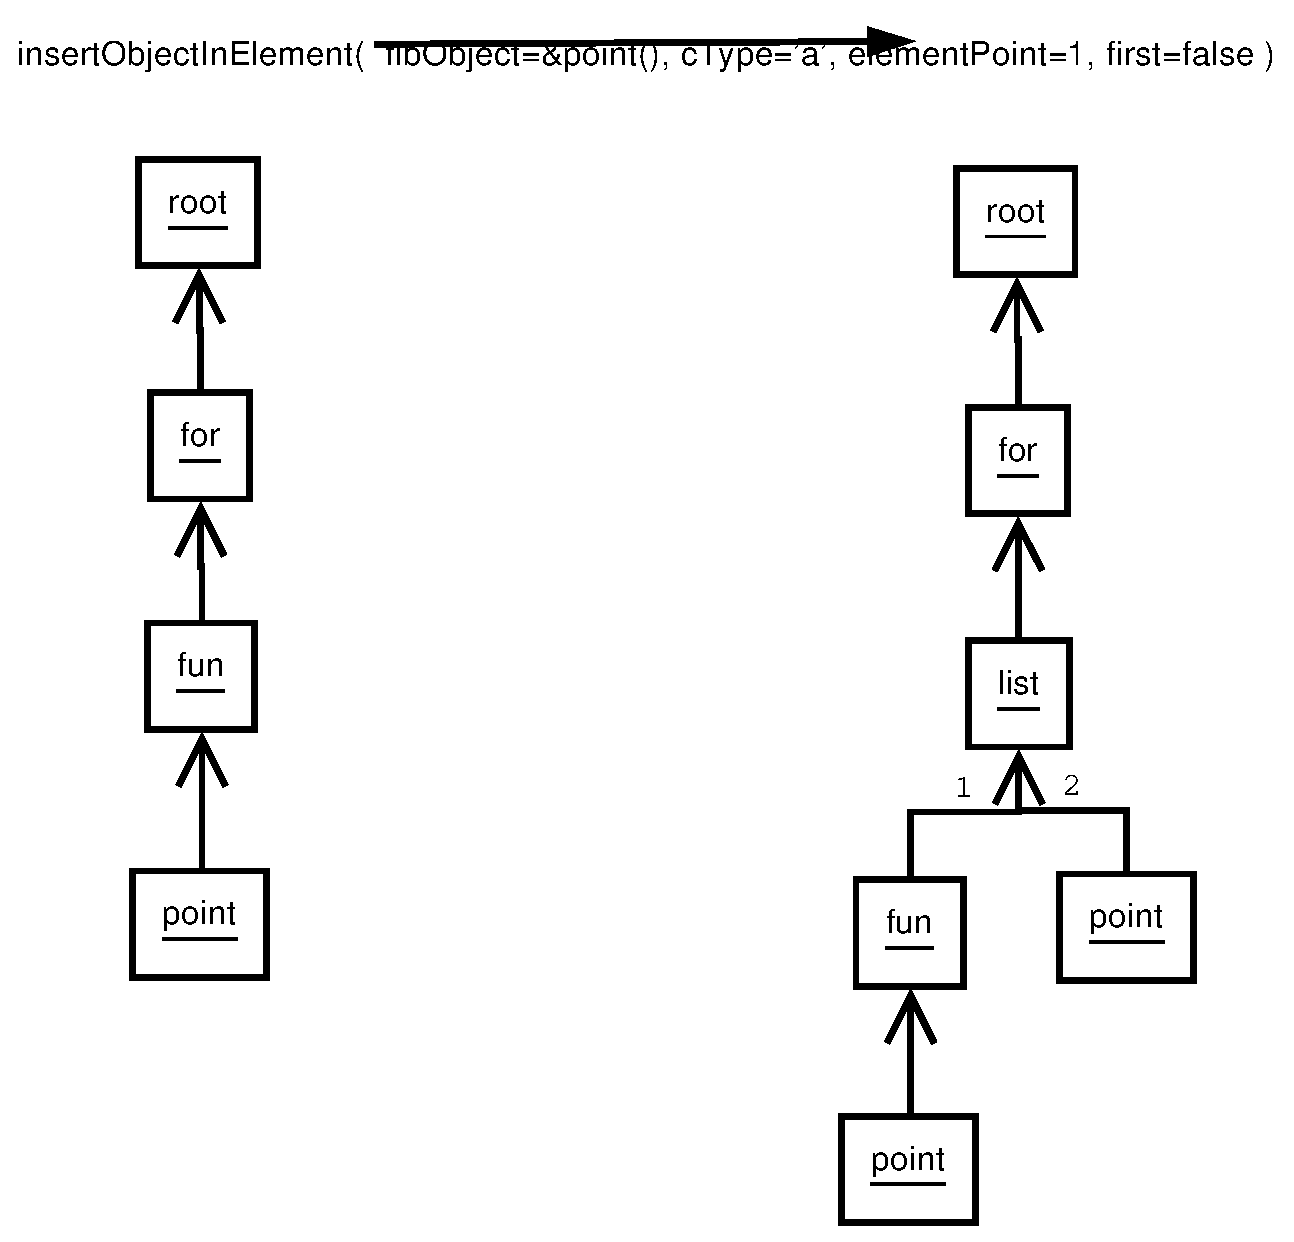
\includegraphics[scale=0.5]{./material_sprachimplementation/insertObjectInElement.eps}
  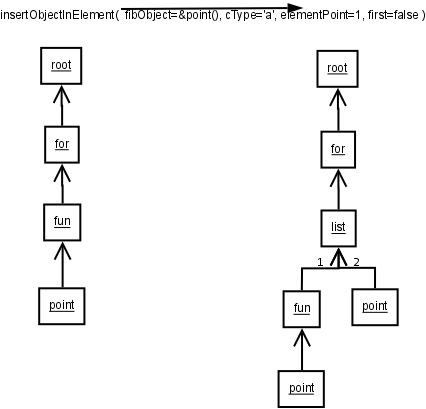
\includegraphics[scale=0.5]{insertObjectInElement}
\end{center}
\caption{Beispiel f"ur insertObjectInElement()}
\label{figInsertObjectInObject}
\end{figure}

%path for pictures
\graphicspath{{./klassendiagramme/}}
\graphicspath{{./klassendiagramme/}{../klassendiagramme}}


\bigskip\noindent
\textbf{Eingabeparameter:}
\begin{itemize}
 \item \verb|fibObject|: Das Fib-Objekt, welches neu unter dem Fib-Element an der angegebenen Position eingef"ugt werden soll.
 \item \verb|cType|: Der Typ des Fib-Elements unter dem das Fib-Objekt \verb|fibObject| eingef"ugt werden soll. Standardm"a"sig werden Fib-Elemente aller Typen betrachtet/gez"ahlt.
 \item \verb|elementPoint|: Die Nummer des Fib-Elements, die es unter den Fib-Elementen vom \verb|cType| haben soll. Standardm"a"sig wird diese mit $0$ belegt und damit das \verb|fibObject| im aktuellem Fib-Element eingef"ugt.
 \item \verb|first|: Wenn \verb|first| gleich \verb|true| (=wahr) ist, wird das \verb|fibObject| als erstes Unterobjekt im (neuem) Listenelement eingesetzt, und damit die anderen Unterobjekte des Listenelements eventuell "uberdeckt. Sonst, wenn \verb|first| gleich \verb|false| (=falsch) ist, wird das \verb|fibObject| als letztes Unterobjekt im Listenelement eingesetzt, und damit eventuell selbst "uberdeckt werden.
 \item \verb|bAbsolute|: Wenn \verb|bAbsolute| gleich \verb|true| (=wahr) ist, bezieht sich die Ordnung auf das gesamte Fib-Objekt. Ansonsten, wenn \verb|bAbsolute| gleich \verb|false| (=falsch) ist, bezieht sich Ordnung auf das Fib-Element, von dem aus die Methode aufgerufen wurde. Der Standardwert ist \verb|false|.
\end{itemize}

\bigskip\noindent
\textbf{R"uckgabe:} Wenn das Fib-Objekt \verb|fibObject| eingef"ugt wurde wird \verb|true| (=wahr) zur"uckgegeben, sonst \verb|false| (=falsch).


\subsubsection{overwriteObjectWithObject}\index{cFibElement!overwriteObjectWithObject()}\index{overwriteObjectWithObject()}

\textbf{Syntax:} \verb|bool overwriteObjectWithObject(| \\\verb| cFibElement* fibObject,| \\\verb| const char cType='u',| \\\verb| unsignedIntFib elementPoint=0 ,| \\\verb| bool bDeleteOld=true,| \\\verb| bool bAbsolute=false )|

\bigskip\noindent
Diese Methode f"ugt das "ubergebene \verb|fibObject| an der angegeben Stelle ein. Das Fib-Element, welches vorher an der Stelle stand, wird entfernt und, wenn \verb|bDeleteOld| gleich \verb|true| (=wahr) ist, gel"oscht (inklusive aller enthaltender Fib-Elemente). Die Position an der das \verb|fibObject| eingef"ugt wird, ist die Position an der vorher das Fib-Element stand, welches das \verb|elementPoint|'te Fib-Element vom angegebenen Typ \verb|cType| ist.

Zur"uckgegeben wird, ob die Operation erfolgreich war. Es kann beispielsweise niemals das aktuelle Fib-Objekt "uberschrieben werden oder anstatt dessen ein neues Fib-Objekt eingef"ugt werden.

\bigskip\noindent
\textbf{Eingabeparameter:}
\begin{itemize}
 \item \verb|fibObject|: Das Fib-Objekt, welches anstatt des Fib-Elements an der angegebenen Position eingef"ugt werden soll.
 \item \verb|cType|: Typ des Fib-Elements, welches durch das Fib-Objekt \verb|fibObject| ersetzt werden soll. Standardm"a"sig werden Fib-Elemente aller Typen betrachtet/gez"ahlt.
 \item \verb|elementPoint|: Die Nummer des Fib-Elements, die es unter den Fib-Elementen vom \verb|cType| haben soll. Standardm"a"sig wird diese mit $0$ belegt und damit das \verb|fibObject| im aktuellem Fib-Element eingef"ugt.
 \item \verb|bDeleteOld|: Wenn \verb|bDeleteOld| gleich \verb|true| (=wahr) ist, wird das alte Fib-Objekt (inklusive enthaltender Fib-Elemente) aus dem Speicher gel"oscht, sonst verbleibt es im Speicher. Standardwert ist \verb|true| (=wahr), um das alte Fib-Objekt zu l"oschen.
 \item \verb|bAbsolute|: Wenn \verb|bAbsolute| gleich \verb|true| (=wahr) ist, bezieht sich die Ordnung auf das gesamte Fib-Objekt. Ansonsten, wenn \verb|bAbsolute| gleich \verb|false| (=False) ist, bezieht sich Ordnung auf das Fib-Element von dem aus die Methode aufgerufen wurde. Der Standardwert ist \verb|false|.
\end{itemize}

\bigskip\noindent
\textbf{R"uckgabe:} Wenn das Fib-Objekt \verb|fibObject| eingef"ugt wurde, wird \verb|true| (=wahr) zur"uckgegeben, sonst \verb|false| (=falsch).


\subsubsection{removeObject}\index{cFibElement!removeObject()}\index{removeObject()}

\textbf{Syntax:} \verb|bool removeObject( unsignedIntFib objectPoint,| \\\verb| bool bDeleteOld=true,| \\\verb| bool bAbsolute=false )|

\bigskip\noindent
Diese Methode entfernt das zusammenh"angenden Teilobjekt, welches die Nummer \verb|objectPoint| in der Ordnung der zusammenh"angenden Teilobjekte hat. F"ur den \verb|objectPoint| sollte es ein Listenobjekt geben, welches eine Unterobjekt enth"alt, welches nur Fib-Elemente des zusammenh"angenden Teilobjekt enth"alt, und dessen andere Unterobjekte, nur Fib-Elemente enthalten die nicht zum zusammenh"angenden Teilobjekt geh"oren. Das Unterobjekt, welches nur Fib-Elemente des zusammenh"angenden Teilobjekt enth"alt, wird aus dem Listenelement entfernt. W"urde das Listenelement nach der Operation nur noch ein Unterobjekt enthalten, wird das entsprechende Listenelement durch das "ubrigbleibende Unterobjekt ersetzt und gel"oscht.

Wenn das echten Objekt mit der Objektpunktnummer \verb|objectPoint| entfernt wurde, wird \verb|true| (=wahr) zur"uckgegeben, sonst \verb|false| (=falsch). Sollte beispielsweise kein zusammenh"angenden Teilobjekt mit der Nummer \verb|objectPoint| existieren oder dieses ein Haup-Fib-Objekt in einem root-Element sein, wird \verb|false| zur"uckgegeben.

Zur Beschreibung der Ordnung von zusammenh"angenden Teilobjekte siehe Abschnitt \ref{secOrderPartobjects} auf Seite \pageref{secOrderPartobjects} .

\bigskip\noindent
\textbf{Eingabeparameter:} 
\begin{itemize}
 \item \verb|objectPoint|: Die Nummer des zu l"oschenden zusammenh"angenden Teilobjekts, welche es unter den zusammenh"angenden Teilobjekten hat.
 \item \verb|bDeleteOld|: Wenn \verb|bDeleteOld| gleich \verb|true| (=wahr) ist, wird das entfernte Fib-Objekt (inklusive enthaltender Fib-Elemente und einem eventuell entfernten Listenelement) aus dem Speicher gel"oscht, sonst verbleibt es im Speicher. Standardwert ist \verb|true| (=wahr), um das alte Fib-Objekt zu l"oschen.
 \item \verb|bAbsolute|: Wenn \verb|bAbsolute| gleich \verb|true| (=wahr) ist, bezieht sich die Ordnung auf das gesamte Fib-Objekt. Ansonsten, wenn \verb|bAbsolute| gleich \verb|false| (=falsch) ist, bezieht sich Ordnung auf das Fib-Element von dem aus die Methode aufgerufen wurde. Standardwert ist \verb|false|.
\end{itemize}

\bigskip\noindent
\textbf{R"uckgabe:} Wenn das zusammenh"angenden Teilobjekt mit der zusammenh"angenden Teilobjektpunktnummer \verb|objectPoint| gel"oscht wurde, wird \verb|true| (=wahr) zur"uckgegeben, sonst \verb|false| (=falsch).


\subsubsection{hasUnderAllObjects}\index{cFibElement!hasUnderAllObjects()}\index{hasUnderAllObjects()}

\textbf{Syntax:} \verb|bool hasUnderAllObjects() const|

\bigskip\noindent
Diese Methode pr"uft, ob in den Fib-Elementen des aktuelle Fib-Objekts alle Unterobjekte vorhanden sind. Sind im Fib-Objekt nicht alle Unterobjekte vorhanden, ist es kein korrektes Fib-Objekt.

\bigskip\noindent
\textbf{Eingabeparameter:} keine

\bigskip\noindent
\textbf{R"uckgabe:} Wenn im Fib-Objekt alle Unterobjekte vorhanden sind, wird \verb|true| (=wahr) zur"uckgegeben, sonst \verb|false| (=falsch).


\subsubsection{isRemovableElement}\index{cFibElement!isRemovableElement()}\index{isRemovableElement()}
\label{secIsRemovableElement}

\textbf{Syntax:} \verb|bool isRemovableElement( const char cType='u', | \\\verb| const unsignedIntFib elementPoint=0,| \\\verb| bool bAbsolute=false ) const|

\bigskip\noindent
Diese Methode "uberpr"uft, ob das Fib-Element vom Typ \verb|cType|, welches die Nummer \verb|elementPoint| in der Ordnung der Fib-Element vom angegebenen Typ \verb|cType| hat, l"oschbar ist.

Blattelemente von der Klasse \verb|cFibLeaf| (z. B. Punkte) und korrekte Verzweigungselemente von der Klasse \verb|cFibBranch| (z. B. Listenelemente) sind niemals l"oschbar. Alle (geraden) Astelemente \verb|cFibLimb| (siehe Abschnitt \ref{secCFibLimb} auf Seite \pageref{secCFibLimb} z. B. Funktions- und Bereichselemente) sind l"oschbar, wenn die Variable, die sie definieren, nirgendwo sonst benutzt wird.

\bigskip\noindent
\textbf{Eingabeparameter:} 
\begin{itemize}
 \item \verb|cType|: Der Typ des Fib-Elements, f"ur welches gepr"uft werden soll, ob es l"oschbar ist. Standardm"a"sig werden Fib-Elemente aller Typen betrachtet/gez"ahlt.
 \item \verb|elementPoint|: Die Nummer des Fib-Elements, die es unter den Fib-Elementen vom \verb|cType| haben soll. Standardm"a"sig wird diese mit $0$ belegt und damit das \verb|fibObject| im aktuellem Fib-Element gel"oscht.
 \item \verb|bAbsolute|: Wenn \verb|bAbsolute| gleich \verb|true| (=wahr) ist, bezieht sich die Ordnung auf das gesamte Fib-Objekt. Ansonsten, wenn \verb|bAbsolute| gleich \verb|false| ist, bezieht sich Ordnung auf das Fib-Element von dem aus die Methode aufgerufen wurde. Standardwert ist \verb|false| (=falsch).
\end{itemize}

\bigskip\noindent
\textbf{R"uckgabe:} Wenn das angegebene Fib-Element vom Typ \verb|cType|, welches die Nummer \verb|elementPoint| in der Ordnung der Fib-Element vom angegebenen Typ \verb|cType| hat, gel"oscht werden kann, wird \verb|true| (=wahr) zur"uckgegeben, sonst \verb|false| (=falsch).


\subsubsection{removeElement}\index{cFibElement!removeElement()}\index{removeElement()}

\textbf{Syntax:} \verb|bool removeElement( const char cType='u', | \\\verb| const unsignedIntFib elementPoint=0,| \\\verb| bool bAbsolute=false )|

\bigskip\noindent
Diese Methode l"oscht das Fib-Element vom Typ \verb|cType|, welches die Nummer \verb|elementPoint| in der Ordnung der Fib-Element vom angegebenen Typ \verb|cType| hat. An der Stelle des Fib-Elements steht nach der Operation das Fib-Element, welches das gel"oschte Fib-Element als Unterobjekt enthalten hat. Es wird also das Fib-Element, das gel"oscht werden soll, durch das Fib-Element, welches es enth"alt, ersetzt und erst dann wird das zu l"oschende Fib-Element gel"oscht. Das Fib-Element kann nicht gel"oscht werden, wenn dadurch ein ung"ultiges Fib-Objekt entstehen w"urde.

Wenn das Fib-Element vom Typ \verb|cType|, mit der Nummer \verb|elementPoint| in der Ordnung der Fib-Element vom angegebenen Typ \verb|cType| , gel"oscht wurde, wird \verb|true| (=wahr) zur"uckgegeben, sonst \verb|false| (=falsch). Sollte beispielsweise versucht werden ein Listenelement zu l"oschen, schl"agt die Operation fehl und es wird \verb|false| zur"uckgegeben, da Listenelemente mindestens zwei Unterobjekte haben, aber nur eins das Listenelement ersetzen k"onnte. Des weiteren k"onnen auch keine Fib-Elemente gel"oscht werden, welche Variablen definieren, die noch ben"otigt werden.
Das aktuelle Fib-Element kann nat"urlich auch nicht gel"oscht werden.

Durch die Methode \verb|isRemovableElement| (siehe Abschnitt \ref{secIsRemovableElement} auf Seite \pageref{secIsRemovableElement} ) kann gepr"uft werden, ob ein Fib-Element l"oschbar ist.

\bigskip\noindent
\textbf{Eingabeparameter:} 
\begin{itemize}
 \item \verb|cType|: Der Typ des Fib-Elements, welches gel"oscht werden soll. Standardm"a"sig (f"ur den Standardwert \verb|'u'|) werden Fib-Elemente aller Typen betrachtet/gez"ahlt.
 \item \verb|elementPoint|: Die Nummer des Fib-Elements, die es unter den Fib-Elementen vom \verb|cType| haben soll. Standardm"a"sig wird diese mit $0$ belegt, damit das erste Fib-Element des ersten Unterobjekts im aktuellem Fib-Element gel"oscht wird.
 \item \verb|bAbsolute|: Wenn \verb|bAbsolute| gleich \verb|true| (=wahr) ist, bezieht sich die Ordnung auf das gesamte Fib-Objekt. Ansonsten, wenn \verb|bAbsolute| gleich \verb|false| ist, bezieht sich Ordnung auf das Fib-Element von dem aus die Methode aufgerufen wurde. Standardwert ist \verb|false| (=falsch).
\end{itemize}

\bigskip\noindent
\textbf{R"uckgabe:} Wenn das entsprechende Fib-Element vom Typ \verb|cType|, welches die Nummer \verb|elementPoint| in der Ordnung der Fib-Element vom angegebenen Typ \verb|cType| hat, gel"oscht wurde, wird \verb|true| (=wahr) zur"uckgegeben, sonst \verb|false| (=falsch).


\subsubsection{cutElement}\index{cFibElement!cutElement()}\index{cutElement()}

\textbf{Syntax:} \verb|cFibElement * cutElement( const char cType='u', | \\\verb| const unsignedIntFib elementPoint=0,| \\\verb| bool bAbsolute=false )|

\bigskip\noindent
Diese Methode entfernt das Fib-Element vom Typ \verb|cType|, welches die Nummer \verb|elementPoint| in der Ordnung der Fib-Element vom angegebenen Typ \verb|cType| hat, aus dem Fib-Objekt und gibt es zur"uck. An der Stelle des Fib-Elements steht nach der Operation, das Fib-Element (Unterobjekt), welches das entfernt Fib-Element enthalten hat. Es wird also das Fib-Element, das entfernt werden soll, durch das Fib-Element, welches es enth"alt, ersetzt und dann das entfernte Fib-Element zur"uckgegeben. Das Fib-Element kann nicht entfernt werden, wenn dadurch ein ung"ultiges Fib-Objekt entstehen w"urde.

Wenn das Fib-Element vom Typ \verb|cType|, mit der Nummer \verb|elementPoint| in der Ordnung der Fib-Element vom angegebenen Typ \verb|cType| , entfernt wurde, wird es bzw. ein Zeiger auf es zur"uckgegeben, sonst wird \verb|NULL| zur"uckgegeben. Sollte beispielsweise versucht werden ein Listenelement zu entfernen, schl"agt die Operation fehl und es wird \verb|NULL| zur"uckgegeben, da Listenelemente mindestens zwei Unterobjekte haben, aber nur eins das Listenelement ersetzen k"onnte. Des weiteren k"onnen auch keine Fib-Elemente entfernt werden, welche Variablen definieren, die noch ben"otigt werden.

\bigskip\noindent
\textbf{Eingabeparameter:}
\begin{itemize}
 \item \verb|cType|: Der Typ des Fib-Elements, welches entfernt werden soll. Standardm"a"sig ('u') werden Fib-Elemente aller Typen betrachtet/ gez"ahlt.
 \item \verb|elementPoint|: Die Nummer des Fib-Elements, die es unter den Fib-Elementen vom \verb|cType| haben soll. Standardm"a"sig wird diese mit $0$ belegt und damit das Fib-Element im aktuellem Fib-Element ausgeschnitten.
 \item \verb|bAbsolute|: Wenn \verb|bAbsolute| gleich \verb|true| (=wahr) ist, bezieht sich die Ordnung auf das gesamte Fib-Objekt. Ansonsten, wenn \verb|bAbsolute| gleich \verb|false| (=falsch) ist, bezieht sich Ordnung auf das Fib-Element von dem aus die Methode aufgerufen wurde. Standardwert ist \verb|false|.
\end{itemize}

\bigskip\noindent
\textbf{R"uckgabe:} Wenn das Fib-Element vom angegebenen Typ \verb|cType|, welches die Nummer \verb|elementPoint| in der Ordnung der Fib-Element vom angegebenen Typ \verb|cType| hat, entfernt wurde, wird es bzw. ein Zeiger auf es zur"uckgegeben, sonst wird \verb|NULL| zur"uckgegeben.


\subsubsection{deleteObject}\index{cFibElement!deleteObject()}\index{deleteObject()}

\textbf{Syntax:} \verb|static void deleteObject( cFibElement * fibObject )|

\bigskip\noindent
Diese Methode l"oscht das gesamte "ubergebene Fib-Objekt \verb|fibObject| mit allen seinen enthaltenden Elementen.
Auf diese Weise muss nicht jedes Fib-Element im Fib-Objekt einzeln "uber seinen Destruktor gel"oscht werden.

Achtung: Existiert das \verb|fibObject| noch in anderen Fib-Elementen bzw. Fib-Objekten werden auch diese mitgel"oscht.

\bigskip\noindent
\textbf{Eingabeparameter:}
\begin{itemize}
 \item \verb|fibObject|: Einen Zeiger auf das zu l"oschende Fib-Objekt.
\end{itemize}

\bigskip\noindent
\textbf{R"uckgabe:} keine


\subsubsection{moveLimbElement}\index{cFibElement!moveLimbElement()}\index{moveLimbElement()}
\label{secMoveLimbElement}

\textbf{Syntax:} \verb|intFib moveLimbElement( const char cType='u', | \\\verb| const unsignedIntFib elementPoint=0,| \\\verb| const intFib iHowfar=1,| \\\verb| bool bAbsolute=false ) |

\bigskip\noindent
Diese Methode verschiebt das Fib-Element vom angegeben Typ \verb|cType|, welches das \verb|elementPoint|'te Fib-Element vom Typ \verb|cType| ist, "uber \verb|iHowfar| Fib-Element. Wenn \verb|iHowfar| positiv ist, wird das Fib-Element nach unten verschoben, sonst nach oben. Es k"onnen nur \verb|cFibLimb| verschoben werden, also nur Fib-Element die genau ein Unterobject haben.

Das Verschieben des Fib-Elements wird abgebrochen, wenn durch ein weiteres Verschieben ein ung"ultiges Fib-Objekt entstehen w"urde. Die Anzahl der Fib-Elemente, "uber die das zu verschiebende Fib-Element verschoben wurde, wird zur"uckgegeben. Wobei der zur"uckgegebene Wert negativ ist, wenn nach oben verschoben wurde. (f"ur die Definition von Oben und Unten siehe Abschnitt \ref{secDefinitionUpDown} auf Seite \pageref{secDefinitionUpDown} )

Ein Fib-Element kann beispielsweise nicht verschoben werden, wenn es ein Punktelement ist oder wenn es "uber ein Fib-Element verschoben werden soll, welches eine Variable definiert, die das zu verschiebende Fib-Element ben"otigt.

Eine besondere Betrachtung beim Verschieben ben"otigt die Verzweigungselemente (\verb|cFibBranch|). Wird ein Fib-Element "uber ein Verzeweigungselemente nach unter verschoben, wandert es in alle Unterobjekte des Verzweigungselemente, in denen es bzw. eine Variable die es definiert ben"otigt wird, wobei in allen au"ser einem Unterobjekt nat"urlich Kopien des Fib-Element verwendet werden. Wird die vom zu verschiebenden Fib-Element definierte Variable in keinem Unterobjekt ben"otigt, wird es nur in das erste Unterobjekt verschoben. Das zu verschiebende Fib-Element wird dann in allen Unterobjekt die noch verbleibenden Schritte $iHowfar-1$ weiter nach unten verschoben. Zur"uckgegeben wird die Summe der Fib-Elemente, "uber die das zu verschiebende Fib-Element oder eine Kopie dessen verschoben wurde.

Auch eine Verschiebung "uber das und vom aktuellem Fib-Element ist m"oglich.

\bigskip\noindent
\textbf{Eingabeparameter:}
\begin{itemize}
 \item \verb|cType|: Der Typ des Fib-Elements, welches verschoben werden soll. Standardm"a"sig werden Fib-Elemente aller Typen betrachtet/ gez"ahlt.
 \item \verb|elementPoint|: Die Nummer des Fib-Elements, die es unter den Fib-Elementen vom \verb|cType| haben soll. Standardm"a"sig wird diese mit $0$ belegt und damit das aktuelle Fib-Element verschoben.
 \item \verb|iHowfar|: Die Anzahl der Fib-Elemente "uber die das zu verschiebende Fib-Element verschoben werden soll. Wenn \verb|iHowfar| positiv ist, wird das Fib-Element nach unten verschoben, sonst nach oben. Standardm"a"sig wird das zu verschiebene Fib-Element um ein Fib-Element nach unter verschoben.
 \item \verb|bAbsolute|: Wenn \verb|bAbsolute| gleich \verb|true| (=wahr) ist, bezieht sich die Ordnung auf das gesamte Fib-Objekt. Ansonsten, wenn \verb|bAbsolute| gleich \verb|false| (=falsch) ist, bezieht sich Ordnung auf das Fib-Element von dem aus die Methode aufgerufen wurde. Standardwert ist \verb|false|.
\end{itemize}

\bigskip\noindent
\textbf{R"uckgabe:} Die Anzahl der Fib-Elemente, "uber die das zu verschiebene Fib-Element verschoben wurde. Wobei der zur"uckgegebene Wert negativ ist, wenn nach oben verschoben wurde, und sonst positiv ist.


\subsubsection{clone}\index{cFibElement!clone()}\index{clone()}

\textbf{Syntax:} \verb|cFibElement *clone() const|

\bigskip\noindent
Diese Methode stellt eine Kopie des gesamten Fib-Objekts her. Dabei werden alle Elemente (auch Vektoren und Variablen) von der Wurzel bzw. dem h"ochsten root-Element an dupliziert.

\bigskip\noindent
\textbf{Eingabeparameter:} keine

\bigskip\noindent
\textbf{R"uckgabe:} Ein Zeiger auf die Kopie des gesamten Fib-Objekts.


\subsubsection{copy}\index{cFibElement!copy()}\index{copy()}

\textbf{Syntax:} \verb|cFibElement *copy(  const unsignedIntFib| \\\verb| iObjectPoint=0 ) const|

\bigskip\noindent
Diese Methode stellt eine Kopie zusammenh"angenden Teilobjekts her, welches das \verb|iObjectPoint|'te unter den zusammenh"angenden Teilobjekten ist. Dabei werden alle Elemente (auch Vektoren und Variablen) von aktuellen Fib-Element an dupliziert, welche zum zusammenh"angenden Teilobjekt geh"oren.

Sollte es kein zusammenh"angenden Teilobjekt mit der Nummer \verb|iObjectPoint| geben, wird der Nullpointer \verb|NULL| zur"uckgegeben.

Variablen die das Fib-Objekt verwendet aber nicht in ihm definiert werden, behalten ihre Referenz auf ihre alte Definition.

\bigskip\noindent
\textbf{Eingabeparameter:}
\begin{itemize}
 \item \verb|iObjectPoint|: Die Nummer, die das zu kopierende zusammenh"angenden Teilobjekt unter den zusammenh"angenden Teilobjekten hat. Standardm"a"sig wir dieser Parameter mit $0$ belegt und damit das gesamte aktuelle Fib-Objekt kopiert.
\end{itemize}

\bigskip\noindent
\textbf{R"uckgabe:} Ein Zeiger auf eine Kopie des zusammenh"angenden Teilobjekts mit der Nummer \verb|iObjectPoint| in der Ordnung der zusammenh"angenden Teilobjekte, oder \verb|NULL|, wenn ein solches zusammenh"angenden Teilobjekt nicht existiert.


\subsubsection{copyElement}\index{cFibElement!copyElement()}\index{copyElement()}

\textbf{Syntax:} \verb|cFibElement *copyElement(  const char cType='u', | \\\verb| const unsignedIntFib elementPoint=0,| \\\verb| bool bAbsolute=false ) const|

\bigskip\noindent
Diese Methode stellt eine Kopie des Fib-Elements vom angegeben Typ \verb|cType| her, welches das \verb|elementPoint|'te Fib-Element vom Typ \verb|cType| ist. Dabei wird das Fib-Element mit seinen enthaltenden Werten und Vektoren aber nicht enthaltende Fib-Elemente kopiert. Verwendete Variablen behalten ihre Referenz bei.

Das zur"uckgegebene Fib-Element hat nach der Kopie den Nullpointer \verb|NULL| f"ur seine (eventuell vorhandenen) Unterobjekte.

Sollte kein Fib-Element an der angegebenen Position existieren, wird der Nullpointer \verb|NULL| zur"uckgegeben.

\bigskip\noindent
\textbf{Eingabeparameter:}
\begin{itemize}
 \item \verb|cType|: Der Typ des Fib-Elements, welches kopiert werden soll. Standardm"a"sig werden Fib-Elemente aller Typen betrachtet/ gez"ahlt.
 \item \verb|elementPoint|: Die Nummer des Fib-Elements, die es unter den Fib-Elementen vom \verb|cType| haben soll. Standardm"a"sig wird diese mit $0$ belegt und damit das aktuellem Fib-Element kopiert.
 \item \verb|bAbsolute|: Wenn \verb|bAbsolute| gleich \verb|true| (=wahr) ist, bezieht sich die Ordnung auf das gesamte Fib-Objekt. Ansonsten, wenn \verb|bAbsolute| gleich \verb|false| (=falsch) ist, bezieht sich Ordnung auf das Fib-Element, von dem aus die Methode aufgerufen wurde. Standardwert ist \verb|false|.
\end{itemize}

\bigskip\noindent
\textbf{R"uckgabe:} Ein Zeiger auf eine Kopie des Fib-Elements an der angegebenen Position, oder \verb|NULL|, wenn ein solches Fib-Element nicht existiert.


\subsubsection{equal}\index{cFibElement!equal()}\index{equal()}

\textbf{Syntax:} \verb|bool equal( const cFibElement* fibObject ) const|

\bigskip\noindent
Diese Methode pr"uft, ob das "ubergebene Fib-Objekt gleich zum aktuellen Fib-Objekt ist. Dabei m"ussen alle Elemente (Fib-Elemente, Vektoren, Werte) und die Struktur gleich sein, bis auf die Referenzen f"ur die Variablen. Referenzen f"ur Variablen m"ussen auf zum "ubergebenen Fib-Objekt entsprechende Definitionen in Fib-Elementen im eigenen Fib-Objekt verweisen.

\noindent
Die folgenden Fib-Objekte sind demanch gleich:
\begin{itemize}
 \item $for( x_1, p(( 1, x_1 )) )$
 \item $for( x_3, p(( 1, x_3 )) )$
\end{itemize}
\noindent
Demgegen"uber sind die Fib-Objekte nicht gleich:
\begin{itemize}
 \item $for( x_1, p(( 1, x_1 )) )$
 \item $fun( x_3, p(( 1, x_3 )) )$
\end{itemize}

Es wird nur das Fib-Objekt unterhalb dem aktuellen und "ubergebenen Fib-Element gepr"uft und Fib-Elemente oberhalb der Fib-Elemente, welche Variablen definieren, die in dem Fib-Objekt unterhalb der Fib-Elemente direkt oder indirekt ben"otigt werden.

\bigskip\noindent
\textbf{Eingabeparameter:}
\begin{itemize}
 \item \verb|fibObject|: Das Fib-Objekt, zu dem das aktuelle Fib-Objekt gleich sein soll.
\end{itemize}

\bigskip\noindent
\textbf{R"uckgabe:} Wenn das aktuelle Fib-Objekt zum "ubergebenen Fib-Objekt gleich ist, wird \verb|true| (=wahr) zur"uckgegeben, sonst \verb|false| (=falsch).


\subsubsection{storeXml}\index{cFibElement!storeXml()}\index{storeXml()}

\textbf{Syntax:} \verb|bool storeXml( ostream& outstream ) const|

\bigskip\noindent
Diese Methode speichert das aktuelle Fib-Objekt im XML-Format in den "ubergebenen \verb|outstream|.

F"ur den Aufbau der XML-Daten siehe Abschnitt \ref{xmlFormat} auf Seite \pageref{xmlFormat}.

\bigskip\noindent
\textbf{Eingabeparameter:}
\begin{itemize}
 \item \verb|outstream|: Der Datenstrom, in dem das Fib-Objekt gespeichert werden soll.
\end{itemize}

\bigskip\noindent
\textbf{R"uckgabe:} Wenn das aktuelle Fib-Objekt erfolgreich gespeichert wurde, wird \verb|true| (=wahr) zur"uckgegeben, sonst \verb|false| (=falsch).


\subsubsection{restoreXml}\index{cFibElement!restoreXml()}\index{restoreXml()}

\textbf{Syntax:} \verb|static cFibElement* restoreXml( | \\\verb| istream& instream , intFib *outStatus=NULL )|

\bigskip\noindent
Diese Methode l"adt ein Fib-Objekt im XML-Format aus dem "ubergebenen \verb|instream| und gibt eine Referenz darauf zur"uck. Konnte das Fib-Objekt nicht erfolgreich geladen werden, wird der Nullpointer \verb|NULL| zur"uckgegeben.

F"ur den Aufbau der XML-Daten siehe Abschnitt \ref{xmlFormat} auf Seite \pageref{xmlFormat}.

\bigskip\noindent
\textbf{Eingabeparameter:}
\begin{itemize}
 \item \verb|instream|: Der Datenstrom, aus dem das Fib-Objekt geladen werden soll.
 \item \verb|outStatus|: Ein Integerfeld zum Speichern des Ladestatus. Standardm"a"sig wird das Feld auf \verb|NULL| gesetzt und damit kein Ladestatus zur"uckgegeben.
\end{itemize}

\bigskip\noindent
\textbf{R"uckgabe:} Wenn das Fib-Objekt erfolgreich geladen wurde, wird ein Zeiger darauf zur"uckgegeben, sonst der Nullpointer \verb|NULL|. Wenn \verb|outStatus| beim Aufruf nicht \verb|NULL| war, steht nach der Ladeoperation der Ladestatus in dieser Variable. Negative Werte sind Fehler und positive Warnungen.

\bigskip\noindent
M"ogliche Werte f"ur \verb|outStatus|:
\begin{itemize}
 \item[0] Laden erfolgreich
 \item[-1] Laden fehlgeschlagen, der Stream \verb|instream| ist ung"ultig
 \item[-2] Laden fehlgeschlagen, Daten sind Fehlerhaft
 \item[1] Daten im Stream \verb|instream| sind Fehlerhaft, Fehler konnten aber korrigiert werden
 \item[2] Daten im Stream \verb|instream| sind Fehlerhaft, Fib-Objekt konnte aber geladen werden; Fehler konnten nicht korrigiert werden, das Multimediaobjekt ist eventuell fehlerhaft
\end{itemize}



\subsubsection{store}\index{cFibElement!store()}\index{store()}

\textbf{Syntax:} \verb|bool store( ostream& outstream ) const|

\bigskip\noindent
Diese Methode speichert das aktuelle Fib-Objekt im komprimierter Form in den "ubergebenen \verb|outstream|.

F"ur den Aufbau der komprimierten Daten siehe Abschnitt \ref{fibCompressing} auf Seite \pageref{fibCompressing}.

\bigskip\noindent
\textbf{Eingabeparameter:}
\begin{itemize}
 \item \verb|outstream|: Der Datenstrom, in dem das Fib-Objekt gespeichert werden soll.
\end{itemize}

\bigskip\noindent
\textbf{R"uckgabe:} Wenn das aktuelle Fib-Objekt erfolgreich gespeichert wurde, wird \verb|true| (=wahr) zur"uckgegeben, sonst \verb|false| (=falsch).


\subsubsection{restore}\index{cFibElement!restore()}\index{restore()}

\textbf{Syntax:} \verb|static cFibElement* restore(| \\\verb| istream& instream , intFib *outStatus=NULL )|

\bigskip\noindent
Diese Methode l"ad ein Fib-Objekt in komprimierter Form aus dem "ubergebenen \verb|instream| und gibt eine Referenz darauf zur"uck. Konnte das Fib-Objekt nicht erfolgreich geladen werden, wird der Nullpointer \verb|NULL| zur"uckgegeben.

F"ur den Aufbau der komprimierten Daten siehe Abschnitt \ref{fibCompressing} auf Seite \pageref{fibCompressing}.

\bigskip\noindent
\textbf{Eingabeparameter:}
\begin{itemize}
 \item \verb|instream|: Der Datenstrom, aus dem das Fib-Objekt geladen werden soll.
 \item \verb|outStatus|: Ein Integerfeld zum Speichern des Ladestatus. Standardm"a"sig wird das Feld auf \verb|NULL| gesetzt und damit kein Ladestatus zur"uckgegeben.
\end{itemize}

\bigskip\noindent
\textbf{R"uckgabe:} Wenn das Fib-Objekt erfolgreich geladen wurde, wird ein Zeiger darauf zur"uckgegeben, sonst der Nullpointer \verb|NULL|. Wenn \verb|outStatus| beim Aufruf nicht \verb|NULL| war, steht nach der Ladeoperation der Ladestatus in dieser Variable. Negative Werte sind Fehler und positive Warnungen.

\bigskip\noindent
M"ogliche Werte f"ur \verb|outStatus|:
\begin{itemize}
 \item[0] Laden erfolgreich
 \item[-1] Laden fehlgeschlagen, der Stream \verb|instream| ist ung"ultig
 \item[-2] Laden fehlgeschlagen, Daten sind Fehlerhaft
 \item[1] Daten im Stream \verb|instream| sind Fehlerhaft, Fehler konnten aber korrigiert werden
 \item[2] Daten im Stream \verb|instream| sind Fehlerhaft, Fib-Objekt konnte aber geladen werden; Fehler konnten nicht korrigiert werden, das Multimediaobjekt ist eventuell fehlerhaft
\end{itemize}



\subsubsection{getAllRootObjectIdentifiers}\index{cFibElement!getAllRootObjectIdentifiers()}\index{getAllRootObjectIdentifiers()}

\textbf{Syntax:} \verb|list<longFib> getAllRootObjectIdentifiers()|

\bigskip\noindent
Diese Methode gibt eine Liste mit den Identifiern aller root-Elementen im gesamten Fib-Objekt und der Datenbank zur"uck.

Dabei k"onnen einige Identifier doppelt auftauchen, wenn sie doppelt im gesamten Fib-Objekt vorhanden sind.

\bigskip\noindent
\textbf{Eingabeparameter:} keine

\bigskip\noindent
\textbf{R"uckgabe:} Eine Liste mit den Identifiern aller root-Objekte im gesamten Fib-Objekt und der Datenbank.


\subsubsection{getAllDatabaseObjectIdentifiers}\index{cFibElement!getAllDatabaseObjectIdentifiers()}\index{getAllDatabaseObjectIdentifiers()}

\textbf{Syntax:} \verb|static list<longFib>| \\\verb| getAllDatabaseObjectIdentifiers()|

\bigskip\noindent
Diese Methode gibt eine Liste mit den Identifiern aller Fib-Objekte in der Fib-Datenbank zur"uck.

\bigskip\noindent
\textbf{Eingabeparameter:} keine

\bigskip\noindent
\textbf{R"uckgabe:} Eine Liste mit den Identifiern aller Fib-Objekte in der Fib-Datenbank.


\subsubsection{getRootObject}\index{cFibElement!getRootObject()}\index{getRootObject}

\textbf{Syntax:} \verb|cRoot * getRootObject( longFib lIdentifier )|

\bigskip\noindent
Diese Methode gibt das root-Objekt zur"uck, welches den angegebenen Identifier \verb|lIdentifier| besitzt. Dabei werden zuerst die vom aktuellem Fib-Element zugreifbaren root-Objekte im aktuellem Fib-Objekt, dann das gesamte Fib-Objekt und dann die Datenbank durchsucht. Wird bei der Suche ein passendes root-Objekt gefunden, wird die Suche abgebrochen und das root-Objekt zur"uckgegeben. Wird kein passendes root-Objekt gefunden, wird \verb|NULL| zur"uckgegeben.

\bigskip\noindent
\textbf{Eingabeparameter:}
\begin{itemize}
 \item \verb|lIdentifier|: Der Identifier, der zum zur"uckzugebenden root-Objekt geh"oren soll.
\end{itemize}

\bigskip\noindent
\textbf{R"uckgabe:} Das root-Objekt das zum \verb|lIdentifier| geh"ort oder \verb|NULL|, wenn kein solches root-Objekt existiert.


\subsubsection{getAllAccessibleRootObjectIdentifiers}\index{cFibElement!getAllAccessibleRootObjectIdentifiers()}\index{getAllAccessibleRootObjectIdentifiers()}

\textbf{Syntax:} \verb|list<longFib>| \\\verb| getAllAccessibleRootObjectIdentifiers()|

\bigskip\noindent
Diese Methode gibt eine Liste mit den Identifiern aller root-Elementen zur"uck, welche vom aktuellem Fib-Element zugreifbar sind. Welche root-Elemente sichbar sind, wird in Abschnitt \ref{secRootOrder} auf Seite \pageref{secRootOrder} beschrieben. Solche root-Elemente k"onnen dann "uber externe Objekte in den aktuellen Fib-Element eingef"ugt werden, siehe Abschnitt \ref{fibExtObject} auf Seite \pageref{fibExtObject} .

\bigskip\noindent
\textbf{Eingabeparameter:} keine

\bigskip\noindent
\textbf{R"uckgabe:} Eine Liste mit den Identifiern aller root-Objekte, welche vom aktuellem Fib-Element zugegriffen werden k"onnen.


\subsubsection{getAccessibleRootObject}\index{cFibElement!getAccessibleRootObject()}\index{getAccessibleRootObject()}

\textbf{Syntax:} \verb|cRoot * getAccessibleRootObject( longFib| \\\verb| lIdentifier )|

\bigskip\noindent
Diese Methode gibt das root-Objekt zur"uck, welches den angegebenen Identifier \verb|lIdentifier| besitzt. Dabei werden nur die vom aktuellen Fib-Element zugreifbaren root-Objekte durchsucht. Welche root-Elemente sichbar sind und in welcher Reihenfolge sie durchsucht werden, wird in Abschnitt \ref{secRootOrder} auf Seite \pageref{secRootOrder} beschrieben. Wird bei der Suche ein passendes root-Objekt gefunden, wird die Suche abgebrochen und das root-Objekt zur"uckgegeben. Wird kein passendes root-Objekt gefunden, wird \verb|NULL| zur"uckgegeben.

\bigskip\noindent
\textbf{Eingabeparameter:}
\begin{itemize}
 \item \verb|lIdentifier|: Der Identifier, der zum zur"uckzugebenden root-Objekt geh"oren soll.
\end{itemize}

\bigskip\noindent
\textbf{R"uckgabe:} Das root-Objekt das zum \verb|lIdentifier| geh"ort oder \verb|NULL|, wenn kein solches root-Objekt vom aktuellen Fib-Element zugreifbar ist.


\subsubsection{getValidDomains}\index{cFibElement!getValidDomains()}\index{getValidDomains()}

\textbf{Syntax:} \verb|cDomains getValidDomains() const|

\bigskip\noindent
Diese Methode gibt eine Referenz auf die Definitionsbereiche, die f"ur das Fib-Element gelten, zur"uck.

\bigskip\noindent
\textbf{Eingabeparameter:} keine

\bigskip\noindent
\textbf{R"uckgabe:} Zur"uckgegeben wird eine Referenz auf die Definitionsbereiche, die f"ur das Fib-Element gelten.


\subsubsection{getNumberOfDimensions}\index{cFibElement!getNumberOfDimensions()}\index{getNumberOfDimensions()}

\textbf{Syntax:} \verb|unsignedIntFib getNumberOfDimensions() const|

\bigskip\noindent
Diese Methode gibt die Anzahl der Dimensionen des Fib-Objekts zur"uck.

\bigskip\noindent
\textbf{Eingabeparameter:} keine

\bigskip\noindent
\textbf{R"uckgabe:} Die Anzahl der Dimensionen des Fib-Objekts.


\subsubsection{getDimensionMapping}\index{cFibElement!getDimensionMapping()}\index{getDimensionMapping()}

\textbf{Syntax:} \verb|unsignedIntFib getDimensionMapping( unsignedIntFib| \\\verb| iDimensionNumber ) const|

\bigskip\noindent
Diese Methode gibt den Mappingwert f"ur die Dimension \verb|iDimensionNumber| zur"uck. Existiert keine solche Dimension, wird $0$ (f"ur ``none'') zur"uckgegeben.

Die Werte werden in Tabelle \ref{tableDimmapValues} auf Seite \pageref{tableDimmapValues} definiert.

\bigskip\noindent
\textbf{Eingabeparameter:}
\begin{itemize}
 \item \verb|iDimensionNumber|: Nummer der Dimension, f"ur welche das Mapping zur"uckgegeben werden soll.
\end{itemize}

\bigskip\noindent
\textbf{R"uckgabe:} Den Mappingwert f"ur die Dimension \verb|iDimensionNumber|, existiert keine solche Dimension wird $0$ zur"uckgegeben.



\section{Das Interface iEvaluePosition}\index{iEvaluePosition}\index{Interface!iEvaluePosition}
\label{secIEvaluePosition}

Das Interface \verb|iEvaluePosition| dient zum Auswerten von Fib-Objekten. Es stellt die Methode \verb|evaluePosition()| bereit.

Jede Klasse die das Interface \verb|iEvaluePosition| implementiert, hat die Methode \verb|evaluePosition()| zu implementieren. Objekte der abgeleiteten Klasse k"onnen dann der Methode \verb|evalueObject()| (siehe Abschnitt \ref{secEvalueObjectPosition} auf Seite \pageref{secEvalueObjectPosition}) "ubergeben werden, um das Fib-Objekt auszuwerten.

Wenn die Methode \verb|evalueObject()| einen Punkt auswertet, ruft sie die Methode \verb|evaluePosition()| des "ubergebenen Objekts mit der Position der Punktes und seinen Eigenschaften auf.


\subsection{evaluePosition}\index{iEvaluePosition!evaluePosition()}\index{evaluePosition()}

\textbf{Syntax:} \verb|bool evaluePosition(| \\\verb| const cVectorPosition & vPosition,| \\\verb| const list<cVectorProperty> & vProperties )|

\bigskip\noindent
Diese Methode wird von der Methode \verb|evalueObject()| (siehe Abschnitt \ref{secEvalueObjectPosition} auf Seite \pageref{secEvalueObjectPosition} ) aufgerufen, wenn ein Punkt ausgewertet werden soll.

\bigskip\noindent
\textbf{Eingabeparameter:}
\begin{itemize}
 \item \verb|vPosition|: Die Position des Punktes, der ausgewertet werden soll.
 \item \verb|vProperties|: Eine Liste mit Eigenschaften des Punktes.
\end{itemize}

\bigskip\noindent
\textbf{R"uckgabe:} Zur"uckgegeben wird \verb|true| (=wahr) wenn die Auswertung vortgesetzt werden soll, sonst false.



\section{Das Interface iEvalueFibElement}\index{iEvalueFibElement}\index{Interface!iEvalueFibElement}
\label{secIEvalueFibElement}

Das Interface \verb|iEvalueFibElement| dient zum Auswerten von Fib-Objekten. Es stellt die Methode \verb|evalueElement()| bereit.

Jede Klasse die das Interface \verb|iEvalueFibElement| implementiert, hat die Methode \verb|evalueElement()| zu implementieren. Objekte der abgeleiteten Klasse k"onnen dann der Methode \verb|evalueObject()| (siehe Abschnitt \ref{secEvalueObjectFibElement} auf Seite \pageref{secEvalueObjectFibElement}) "ubergeben werden, um das Fib-Objekt auszuwerten.

Wenn die Methode \verb|evalueObject()| ein Fib-Element, vom angegeben Type oder ein Punktelement, auswertet, ruft sie die Methode \verb|evalueElement()| des "ubergebenen Objekts mit einem Zeiger auf des Fib-Element und seinen Eigenschaften auf.


\subsection{evaluePosition}\index{iEvalueFibElement!evaluePosition()}\index{evaluePosition()}

\textbf{Syntax:} \verb|bool evalueElement( cFibElement & pFibElement,| \\\verb| const list<cVectorProperty> & vProperties )|

\bigskip\noindent
Diese Methode wird von der Methode \verb|evalueObject()| (siehe Abschnitt \ref{secEvalueObjectFibElement} auf Seite \pageref{secEvalueObjectFibElement} ) aufgerufen, wenn ein Fib-Element, vom angegeben Type oder ein Punktelement, ausgewertet werden soll.

\bigskip\noindent
\textbf{Eingabeparameter:}
\begin{itemize}
 \item \verb|pFibElement|: Eine Refernz auf das Fib-Element, welches ausgewertet werden soll.
 \item \verb|vProperties|: Eine Liste mit Eigenschaften des Fib-Elements.
\end{itemize}

\bigskip\noindent
\textbf{R"uckgabe:} Zur"uckgegeben wird \verb|true| (=wahr) wenn die Auswertung vortgesetzt werden soll, sonst false.



\section{Abh"angigkeiten}\index{Abh"angigkeiten}


Jedes Fib-Element (auch die root-Elemente) h"alt jeweils eine Referenzen auf sein Vorg"anger-, Nachfolger-, n"achst h"oheres Fib-Element und n"achst h"oheres root-Element. Das zu einem Fib-Element geh"orende root-Element ist das n"achste root-Element, welches das Fib-Element enth"alt. die Vorg"anger- und Nachfolgerelemente sind die entsprechenden Elemente in der Ordnung der Fib-Elemente (siehe Abschnitt \ref{secOrderFibElements} auf Seite \pageref{secOrderFibElements}).

Um zu gew"ahrleisten, dass ein Fib-Element immer die Referenz auf das richtige Vorg"anger-, Nachfolger-, n"achst h"oheres Fib-Element und root-Element h"alt, registriert sich ein neues Fib-Element oder -Objekt beim gesamten Fib-Objekten. Die Registrierung wird an alle Fib-Elemente weitergegeben, welche jeweils ihre abh"angigen Referenzen und Daten aktualisieren.


\section{cFibLeaf}\index{cFibLeaf}

Die Klasse \verb|cFibLeaf| ist die Elternklasse f"ur alle Fib-Elementklassen die Bl"atter sind, also kein Unterobjekt einthalten. Von \verb|cFibLeaf| selbst k"onnen keine Instnzen erzeugt werden.

\bigskip\noindent
\textbf{Elternklasse:} \verb|cFibElement|

\bigskip\noindent
Die Abgeleiteten Klassen sind:
\begin{itemize}
 \item \verb|cPoint|
 \item \verb|cExtSubobject|
\end{itemize}


\section{cFibLimb}\index{cFibLimb}
\label{secCFibLimb}

Die Klasse \verb|cFibLimb| ist die Elternklasse f"ur alle Fib-Elementklassen die (gerade) Zweige sind, also genau ein Unterobjekt enthalten. Von \verb|cFibLimb| selbst k"onnen keine Instnzen erzeugt werden.

\bigskip\noindent
\textbf{Elternklasse:} \verb|cFibElement|

\bigskip\noindent
Die Abgeleiteten Klassen sind:
\begin{itemize}
 \item \verb|cProperty|
 \item \verb|cList|
 \item \verb|cComment|
 \item \verb|cArea|
 \item \verb|cFunction|
 \item \verb|cIf|
\end{itemize}


\section{cFibBranch}\index{cFibBranch}
\label{secCFibBranch}

Die Klasse \verb|cFibBranch| ist die Elternklasse f"ur alle Fib-Elementklassen die Verzweigungen darstellen, also mehrere Unterobjekte haben k"onnen. Von der Klasse \verb|cFibBranch| selbst k"onnen keine Instnzen erzeugt werden.

\bigskip\noindent
\textbf{Elternklasse:} \verb|cFibElement|

\bigskip\noindent
Die Abgeleiteten Klassen sind:
\begin{itemize}
 \item \verb|cList|
 \item \verb|cIf|
 \item \verb|cRoot|
 \item \verb|cExtObject|
\end{itemize}


\section{cPoint}\index{Punktelement}\index{cPoint}

Die Klasse \verb|cPoint| realisiert das Punktelement.
Zur Beschreibung des Punktelements siehe Abschnitt \ref{fibPoint} auf Seite \pageref{fibPoint} .

\bigskip\noindent
\textbf{Elternklasse:} \verb|cFibLeaf|


\subsection{Schnittstellenbeschreibung}


\subsubsection{cPoint}\index{cPoint}

\textbf{Syntax:} \verb|cPoint( const cVectorPosition *vecPositon=NULL )|

\bigskip\noindent
Der Konstruktor des Punktelements, er erstellt einen Punkt. Eine Kopie eines eventuell "ubergebene Positionsvektor wird als Position des Punktes eingesetzt.

\bigskip\noindent
\textbf{Eingabeparameter:}
\begin{itemize}
 \item \verb|vecPositon|: Einen Zeiger auf den Positionsvektor, den der erzeugte Punkt erhalten soll. Standardm"a"sig wird \verb|NULL| "ubergeben. Ist der Positionsvektor \verb|NULL| wird ein Punkt ohne Positionsvektor erzeugt (der Punkt hat keine Auswirkungen) .
\end{itemize}

\bigskip\noindent
\textbf{R"uckgabe:} keine


\subsubsection{getPosition}\index{cPoint!getPosition()}\index{getPosition()}

\textbf{Syntax:} \verb|cVectorPosition *getPosition()|

\bigskip\noindent
"Uber diese Methode kann der Positionsvektor des Punktes ermittelt werden.

\bigskip\noindent
\textbf{Eingabeparameter:} keine

\bigskip\noindent
\textbf{R"uckgabe:} Eine Referenz auf den Positionsvektor des Punktes oder \verb|NULL|, wenn der Punkt keinen Positionsvektor enth"alt.


\subsubsection{setPosition}\index{cPoint!setPosition()}\index{setPosition()}

\textbf{Syntax:} \verb|void setPosition( const cVectorPosition| \\\verb| *vecPositon=NULL )|

\bigskip\noindent
"Uber diese Methode kann der Positionsvektor des Punktes gesetzt werden. Eine Kopie eines eventuell "ubergebene Positionsvektor wird als Position des Punktes eingesetzt. Wird kein Positionsvektor (\verb|NULL|) "ubergeben, hat der Punkt keinen Positionsvektor (der Punkt hat keine Auswirkungen) .

\bigskip\noindent
\textbf{Eingabeparameter:}
\begin{itemize}
 \item \verb|vecPositon|: Einen Zeiger auf den Positionsvektor, den der Punkt erhalten soll. Standardm"a"sig wird \verb|NULL| "ubergeben. Ist der Positionsvektor \verb|NULL|, entsteht ein Punkt ohne Positionsvektor (der Punkt hat keine Auswirkungen).
\end{itemize}

\bigskip\noindent
\textbf{R"uckgabe:} keine


\section{cProperty}\index{Eigenschaftselement}\index{cProperty}

Die Klasse \verb|cProperty| realisiert das Eigenschaftselement.
Zur Beschreibung des Eigenschaftselements siehe Abschnitt \ref{fibProperty} auf Seite \pageref{fibProperty} .

\bigskip\noindent
\textbf{Elternklasse:} \verb|cFibLimb|


\subsection{Schnittstellenbeschreibung}


\subsubsection{cProperty}

\textbf{Syntax:} \verb|cProperty( const cVectorProperty &vecProperty,| \\\verb| cFibElement *pFibUnderObject )|

\bigskip\noindent
Der Konstrukter des Eigenschaftselements, er erstellt einen Eigenschaftselement. Eine Kopie eines "ubergebene Eigenschaftsvektors \verb|vecProperty| wird als Eigenschaft des Eigenschaftselements eingesetzt.

Von den "ubergebenen Unterobjekten \verb|pFibUnderObject| wird keine Kopie erstellt, daher darf es nicht einfach gel"oscht werden.

\bigskip\noindent
\textbf{Eingabeparameter:}
\begin{itemize}
 \item \verb|vecProperty|: Der einzusetzende Eigenschaftsvektor, den das erzeugte Eigenschaftselement erhalten soll.
 \item \verb|pFibUnderObject|: Ein Zeiger auf das einzusetzende Unterobjekt, den das erzeugte Eigenschaftselement enhalten soll. Der Standardwert ist \verb|NULL|. Ist der Wert \verb|NULL|, hat das Eigenschaftselement zun"achst kein Unterobjekt, dieses muss dann sp"ater gesetzt werden.
\end{itemize}

\bigskip\noindent
\textbf{R"uckgabe:} keine


\subsubsection{getProperty}\index{cProperty!getProperty()}\index{getProperty()}

\textbf{Syntax:} \verb|cVectorProperty *getProperty()|

\bigskip\noindent
"Uber diese Methode kann der Eigenschaftsvektor der Eigenschaft ermittelt werden.

\bigskip\noindent
\textbf{Eingabeparameter:} keine

\bigskip\noindent
\textbf{R"uckgabe:} Eine Referenz auf den Eigenschaftsvektor der Eigenschaft.


\section{cList}\index{Listenelement}\index{cList}

Mit der Klasse \verb|cList| wird das Listenelement realisiert.
Zur Beschreibung des Listenelements siehe Abschnitt \ref{fibList} auf Seite \pageref{fibList} .

\bigskip\noindent
\textbf{Elternklasse:} \verb|cFibBranch|


\subsection{Schnittstellenbeschreibung}

\subsubsection{cList}

\textbf{Syntax:} \verb|cList( cFibElement * fibObject1,| \\\verb| cFibElement * fibObject2 )|

\bigskip\noindent
Der Konstruktor des Listenelements, er erstellt einen Listenobjekt. Die erstellte Liste hat die beiden "ubergebenen Fib-Objekte als Teilobjekte.
Von den "ubergebenen Unterobjekten \verb|fibObject1| und \verb|fibObject2| wird keine Kopie erstellt, sie d"urfen daher nicht einfach gel"oscht werden.

\bigskip\noindent
\textbf{Eingabeparameter:}
\begin{itemize}
 \item \verb|fibObject1|: Ein Zeiger auf das erste Fib-Objekt bzw. Unterobjekt des erstellten Listenobjekts.
 \item \verb|fibObject2|: Ein Zeiger auf das zweite Fib-Objekt bzw. Unterobjek des erstellten Listenobjekts.
\end{itemize}

\bigskip\noindent
\textbf{R"uckgabe:} keine


\subsubsection{getNumberOfUnderObjects}\index{cList!getNumberOfUnderObjects()}\index{getNumberOfUnderObjects()}

\textbf{Syntax:} \verb|unsignedIntFib getNumberOfUnderObjects() const|

\bigskip\noindent
Diese Methode gibt die Anzahl der Unterobjekt im aktuellen Listenelement zur"uck.

\bigskip\noindent
\textbf{Eingabeparameter:} keine

\bigskip\noindent
\textbf{R"uckgabe:} Die Anzahl der Unterobjekt im aktuellen Listenelement.


\subsubsection{getUnderObject}\index{cList!getUnderObject()}\index{getUnderObject()}

\textbf{Syntax:} \verb|cFibElement* getUnderObject( unsignedIntFib| \\\verb| iNumberOfUnderObject=1 )|

\bigskip\noindent
Diese Methode gibt das \verb|iNumberOfUnderObject|'te Unterobjekt des Listenelement zur"uck.

\bigskip\noindent
\textbf{Eingabeparameter:} 
\begin{itemize}
 \item \verb|iNumberOfUnderObject|: Die Nummer des Unterobjekts in der Liste des Listenelements, welches zur"uckgegeben werden soll. Wird keine Nummer angegeben, wird das erste Unterobjekt aus der Liste zur"uckgegeben.
\end{itemize}

\bigskip\noindent
\textbf{R"uckgabe:} Das \verb|iNumberOfUnderObject|'te Unterobjekt des Listenelement oder \verb|NULL|, wenn kein \verb|iNumberOfUnderObject|'tes Unterobjekt existiert.


\subsubsection{addUnderObject}\index{cList!addUnderObject()}\index{addUnderObject()}

\textbf{Syntax:} \verb|bool addUnderObject( cFibElement * pUnderObject,| \\\verb| unsignedIntFib iPosition=1 )|

\bigskip\noindent
Diese Methode f"ugt das "ubergebene Fib-Objekt \verb|pUnderObject| an der Stelle \verb|iPosition| in der Unterobjektliste ein.

Von den "ubergebenen Unterobjekt \verb|pUnderObject| wird keine Kopie erstellt, es darf daher nicht einfach gel"oscht werden.

\bigskip\noindent
\textbf{Eingabeparameter:}
\begin{itemize}
 \item \verb|pUnderObject|: Ein Zeiger auf das Unterobjekt, welches in die Liste eingef"ugt werden soll.
 \item \verb|iPosition|: Die Position, an der das Unterobjekt in die Liste eingef"ugt werden soll. Wird keine Nummer angegeben, wird das Unterobjekt als Erstes in der Liste eingef"ugt. Ist die "ubergebene Zahl gr"o"ser als die Anzahl der Unterobjekte in der Liste, wird das "ubergebene Unterobjekt \verb|pUnderObject| als letztes an die Liste angeh"angt.
\end{itemize}

\bigskip\noindent
\textbf{R"uckgabe:} Es wird \verb|true| (=wahr) zur"uck gegeben, wenn das "ubergebene Unterobjekt \verb|pUnderObject| in die Liste eingef"ugt wurde, sonst \verb|false| (=falsch).


\subsubsection{deleteUnderObject}\index{cList!deleteUnderObject()}\index{deleteUnderObject()}

\textbf{Syntax:} \verb|bool deleteUnderObject( unsignedIntFib| \\\verb| iPositionUnderObject, bool bDeleteOld=true )|

\bigskip\noindent
Diese Methode l"oscht das Unterobjekt an der Stelle \verb|iPositionUnderObject| in der Unterobjektliste. 

Dabei k"onnen alle bis auf zwei Unterobjekt aus der Liste gel"oscht werden. Da ein Listenobjekt mit weniger als zwei Unterobjekten kein g"ultiges Fib-Objekt mehr darstellt. Soll dennoch nur noch ein Unterobjekt verwendet werden, ist das Listenelement (das Fib-Element) zu l"oschen.

\bigskip\noindent
\textbf{Eingabeparameter:} 
\begin{itemize}
 \item \verb|iPositionUnderObject|: Die Position, von der das Unterobjekt aus der Liste gel"oscht werden soll. Ist die "ubergebene Zahl gr"o"ser als die Anzahl der Unterobjekte in der Liste oder $0$, wird kein Unterobjekt gel"oscht.
 \item \verb|bDeleteOld|: Wenn \verb|bDeleteOld| gleich \verb|true| (=wahr) ist, wird das entfernte Fib-Objekt (inklusive enthaltender Fib-Elemente) aus dem Speicher gel"oscht, sonst verbleibt es im Speicher. Standardwert ist \verb|true| (=wahr), um das alte Fib-Objekt zu l"oschen.

\end{itemize}

\bigskip\noindent
\textbf{R"uckgabe:} Es wird \verb|true| (=wahr) zur"uck gegeben, wenn aus der Liste das entsprechende \verb|iPositionUnderObject|'te Unterobjekt gel"oscht wurde, sonst wird \verb|false| (=falsch) zur"uck gegeben.


\section{cComment}\index{Anmerkungselement}\index{cComment}

Die Klasse \verb|cComment| realisiert das Anmerkungselement.
Zur Beschreibung des Anmerkungselements siehe Abschnitt \ref{fibComment} auf Seite \pageref{fibComment} .

\bigskip\noindent
\textbf{Elternklasse:} \verb|cFibLimb|


\subsection{Schnittstellenbeschreibung}

\subsubsection{cComment}

\textbf{Syntax:} \verb|cComment( const string szKey, const string| \\\verb| szValue, cFibElement * pFibUnderObject )|

\bigskip\noindent
Der Konstruktor des Anmerkungselements, er erstellt einen Anmerkungselement.

Von den "ubergebenen Unterobjekten \verb|pFibUnderObject| wird keine Kopie erstellt, daher darf es nicht einfach gel"oscht werden.

\bigskip\noindent
\textbf{Eingabeparameter:}
\begin{itemize}
 \item \verb|szKey|: Der einzusetzende Schl"ussel, den das erzeugte Anmerkungselement erhalten soll.
 \item \verb|szValue|: Der einzusetzende Wert, den das erzeugte Anmerkungselement erhalten soll.
 \item \verb|pFibUnderObject|: Ein Zeiger auf das einzusetzende Unterobjekt, den das erzeugte Anmerkungselement enthalten soll. Ist der Wert \verb|NULL|, hat das Anmerkungselement zun"achst kein Unterobjekt, dieses muss dann sp"ater gesetzt werden.
\end{itemize}

\bigskip\noindent
\textbf{R"uckgabe:} keine


\subsubsection{getKey}\index{cComment!getKey()}\index{getKey()}

\textbf{Syntax:} \verb|string getKey() const|

\bigskip\noindent
Diese Methode liefert den Schl"ussel des Kommentars zur"uck.

\bigskip\noindent
\textbf{Eingabeparameter:} keine

\bigskip\noindent
\textbf{R"uckgabe:} Der Schl"ussel des Kommentars.


\subsubsection{setKey}\index{cComment!setKey()}\index{setKey()}

\textbf{Syntax:} \verb|void setKey( const string szKey )|

\bigskip\noindent
Diese Methode setzt den Schl"ussel des Kommentars auf \verb|szKey|.

\bigskip\noindent
\textbf{Eingabeparameter:}
\begin{itemize}
 \item \verb|szKey|: Der Schl"ussel den das Kommentar haben soll.
\end{itemize}

\bigskip\noindent
\textbf{R"uckgabe:} keine


\subsubsection{getValue}\index{cComment!getValue()}\index{getValue()}

\textbf{Syntax:} \verb|string getValue() const|

\bigskip\noindent
Diese Methode liefert den Wert des Kommentars zur"uck.

\bigskip\noindent
\textbf{Eingabeparameter:} keine

\bigskip\noindent
\textbf{R"uckgabe:} Der Wert des Kommentars.


\subsubsection{setValue}\index{cComment!setValue()}\index{setValue()}

\textbf{Syntax:} \verb|void setValue( const string szValue )|

\bigskip\noindent
Diese Methode setzt den Wert des Kommentars auf \verb|szValue|.

\bigskip\noindent
\textbf{Eingabeparameter:}
\begin{itemize}
 \item \verb|szValue|: Der Wert den das Kommentar haben soll.
\end{itemize}

\bigskip\noindent
\textbf{R"uckgabe:} keine


\section{cArea}\index{Bereichselement}\index{cArea}

Die Klasse \verb|cArea| realisiert das Bereichselement.
Zur Beschreibung des Bereichselement siehe Abschnitt \ref{fibArea} auf Seite \pageref{fibArea} .

Zu beachten ist, dass die Reihenfolge der Unterbereiche eines Bereichselements durch "Uberdeckungen Auswirkungen auf das angezeigte Multimediaobjekt haben kann. Darauf sollte beispielsweise geachtet werden, wenn neue Unterbereiche eingef"ugt oder die Unterbereiche sortiert werden.

\bigskip\noindent
\textbf{Elternklasse:} \verb|cFibLimb|


\subsection{Schnittstellenbeschreibung}

\subsubsection{cArea}

\textbf{Syntax:} \verb|cArea( const cVectorArea &vecSubarea,| \\\verb| cFibElement * pFibUnderObject )|

\bigskip\noindent
Der Konstruktor des Bereichselements, er erstellt einen Bereichselement.

Von den "ubergebenen Unterobjekten \verb|pFibUnderObject| wird keine Kopie erstellt, daher darf es nicht einfach gel"oscht werden.

\bigskip\noindent
\textbf{Eingabeparameter:}
\begin{itemize}
 \item \verb|vecSubarea|: Der einzusetzende Bereich, den das erzeugte Bereichselement erhalten soll. Von diesem wird eine Kopie in das neue Bereichselement eingef"ugt.
 \item \verb|pFibUnderObject|: Ein Zeiger auf das einzusetzende Unterobjekt, den das erzeugte Bereichselement enthalten soll. Ist der Wert \verb|NULL|, hat das Bereichselement zun"achst kein Unterlobjekt, dieses muss dann sp"ater gesetzt werden. Das Fib-Objekt \verb|pFibUnderObject| wird direkt in das neue Bereichselement als Unterobjekt eingef"ugt, ohne dass davon eine Kopie erstellt wird.
\end{itemize}

\bigskip\noindent
\textbf{R"uckgabe:} keine


\subsubsection{getNumberOfSubareas}\index{cArea!getNumberOfSubareas()}\index{getNumberOfSubareas()}

\textbf{Syntax:} \verb|unsignedIntFib getNumberOfSubareas() const|

\bigskip\noindent
Diese Methode liefert die Anzahl der Teilbereiche zur"uck.

\bigskip\noindent
\textbf{Eingabeparameter:} keine

\bigskip\noindent
\textbf{R"uckgabe:} Die Anzahl der Teilbereiche.


\subsubsection{getSubarea}\index{cArea!getSubarea()}\index{getSubarea()}

\textbf{Syntax:} \verb|cVectorArea * getSubarea(| \\\verb| unsignedIntFib iSubarea=1 )|

\bigskip\noindent
Diese Methode liefert ein Zeiger auf den \verb|iSubarea|'ten Teilbereich zur"uck (die Z"ahlung beginnt bei 1).

\bigskip\noindent
\textbf{Eingabeparameter:}
\begin{itemize}
 \item \verb|iSubarea|: Die Nummer des Teilbereichs der zur"uckgegeben werden soll. Wird kein Wert angegeben wird der erste Teilbereiche zur"uckgegeben. (Der Standardwert ist $1$ .)
\end{itemize}

\bigskip\noindent
\textbf{R"uckgabe:} Den \verb|iSubarea|'ten Teilbereich oder \verb|NULL|, wenn kein entsprechender \verb|iSubarea|'ter Teilbereich existiert.


\subsubsection{addSubarea}\index{cArea!addSubarea()}\index{addSubarea()}

\textbf{Syntax:} \verb|bool addSubarea( const cVectorArea & underArea,| \\\verb| unsignedIntFib uiPosition=0 )|

\bigskip\noindent
Diese Methode f"ugt den "ubergebenen Teilbereich dem Bereich hinzu. Der Teilbereich wird an der \verb|uiPosition|'ten Stelle in der Liste der Teilbereich hinzugef"ugt.

\bigskip\noindent
\textbf{Eingabeparameter:}
\begin{itemize}
 \item \verb|underArea|: Der Teilbereich, der zum Bereich hinzugef"ugt werden soll. Von diesem wird eine Kopie als neuer Teilbereich eingef"ugt.
 \item \verb|uiPosition|: Die Position, an welcher der Teilbereich \verb|underArea| in der Liste der Teilbereich hinzugef"ugt werden soll. Wenn dieser Wert $0$ oder gr"o"ser der Anzahl der Teilbereich ist, wird der Teilbereich \verb|underArea| an das Ende der Liste der Teilbereich hinzugef"ugt. Standardwert ist $0$, um den Teilbereich \verb|underArea| an das Ende der Liste der Teilbereich hinzuzuf"ugen.
\end{itemize}

\bigskip\noindent
\textbf{R"uckgabe:} Es wird \verb|true| (=wahr) zur"uck gegeben, wenn der "ubergebene Teilbereich \verb|underArea| zum Bereich hinzugef"ugt wurde, sonst \verb|false| (=falsch).


\subsubsection{deleteSubarea}\index{cArea!deleteSubarea()}\index{deleteSubarea()}

\textbf{Syntax:} \verb|bool deleteSubarea(| \\\verb| unsignedIntFib uiSubareaPosition )|

\bigskip\noindent
Diese Methode l"oscht den \verb|uiSubareaPosition|'ten Teilbereich aus dem Bereich. Es k"onnen alle Teilbereich gel"oscht werden, solange danach noch ein Teilbereich vorhanden ist.

\bigskip\noindent
\textbf{Eingabeparameter:}
\begin{itemize}
 \item \verb|uiSubareaPosition|: Die Nummer des Teilbereichs, der aus dem Bereich gel"oscht werden soll.
\end{itemize}

\bigskip\noindent
\textbf{R"uckgabe:} Es wird \verb|true| (=wahr) zur"uck gegeben, wenn der Teilbereich an der Position \verb|uiSubareaPosition| aus dem Bereich gel"oscht wurde, sonst wird \verb|false| (=falsch) zur"uckgegeben.


\subsubsection{sort}\index{cArea!sort()}\index{sort()}

\textbf{Syntax:} \verb|bool sort()|

\bigskip\noindent
Diese Methode ordnet die Teilbereiche des Bereichs.

\bigskip\noindent
Zum Ordnen geh"ort:
\begin{itemize}
 \item Bei allen Teilbereich deren Grenzen zwei Werte sind, ist der erste Wert kleiner als der zweite.
 \item Zwei Teilbereich, deren Grenzen jeweils zwei Werte sind und die sich "uberschneiden, werden zu einem zusammengefasst.
 \item Die Liste der Werte der Teilbereiche ist aufsteigend sortiert. (Teilbereiche mit kleineren Grenzwerten kommen vor Teilbereichen mit gr"o"seren Grenzwerten.)
\end{itemize}

Variablen k"onnen nat"urlich beim Ordnen nicht ber"ucksichtigt werden. (Da ihr Wert unbekannt ist.)

\bigskip\noindent
\textbf{Eingabeparameter:} keine

\bigskip\noindent
\textbf{R"uckgabe:} Es wird \verb|true| (=wahr) zur"uck gegeben, wenn die Teilbereiche im Bereich geordnet wurden, sonst \verb|false| (=falsch).


\subsubsection{getDefinedVariable}\index{cArea!getDefinedVariable()}\index{getDefinedVariable()}

\textbf{Syntax:} \verb|cFibVariable * getDefinedVariable()|

\bigskip\noindent
Diese Methode gibt einen Zeiger auf die vom Bereichsobjekt definierte Variable zur"uck.

Diese Variable kann im gesamten Unterobjekt des Bereichselements verwendet/ eingesetzt werden. Bei der Auswertung wird die Variable nacheinander mit den Werten des Bereichs belegt.

\bigskip\noindent
\textbf{Eingabeparameter:} keine

\bigskip\noindent
\textbf{R"uckgabe:} Es wird ein Zeiger auf die vom Bereichsobjekt definierte Variable zur"uckgegeben.


\section{cFunction}\index{Funktionselement}\index{cFunction}

Die Klasse \verb|cFunction| implementiert das Funktionselement.
Zur Beschreibung des Funktionselements siehe Abschnitt \ref{fibFunction} auf Seite \pageref{fibFunction} .

\bigskip\noindent
\textbf{Elternklasse:} \verb|cFibLimb|


\subsection{Schnittstellenbeschreibung}

\subsubsection{cFunction}

\textbf{Syntax:} \verb|cFunction(| \\\verb| const cUnderFunction &underFunction,| \\\verb| cFibElement * pFibUnderObject )|

\bigskip\noindent
Der Konstruktor des Funktionselements, er erstellt einen Funktionselement.

Von den "ubergebenen Unterobjekten \verb|pFibUnderObject| wird keine Kopie erstellt, daher darf es nicht einfach gel"oscht werden.

\bigskip\noindent
\textbf{Eingabeparameter:}
\begin{itemize}
 \item \verb|underFunction|: Die einzusetzende Unterfunktion, welche das erzeugte Funktionselement erhalten soll. Von diesem wird eine Kopie in das neue Funktionselement eingef"ugt.
 \item \verb|pFibUnderObject|: Ein Zeiger auf das einzusetzende Unterobjekt, den das erzeugte Funktionselement enthalten soll. Ist der Wert \verb|NULL|, hat das Funktionselement zun"achst kein Unterobjekt, dieses muss dann sp"ater gesetzt werden. Das Fib-Objekt \verb|pFibUnderObject| wird direkt in das neue Funktionselement als Unterobjekt eingef"ugt, ohne dass davon eine Kopie erstellt wird.
\end{itemize}

\bigskip\noindent
\textbf{R"uckgabe:} keine


\subsubsection{getDefinedVariable}\index{cFunction!getDefinedVariable()}\index{getDefinedVariable()}

\textbf{Syntax:} \verb|cFibVariable* getDefinedVariable()|

\bigskip\noindent
Diese Methode gibt die Variable zur"uck, welche von der Funktion definiert wird.

\bigskip\noindent
\textbf{Eingabeparameter:} keine

\bigskip\noindent
\textbf{R"uckgabe:} Die Variable, welche von der Funktion definiert wird.


\subsubsection{getUnderFunction}\index{cFunction!getUnderFunction()}\index{getUnderFunction()}

\textbf{Syntax:} \verb|cUnderFunction * getUnderFunction()|

\bigskip\noindent
Diese Methode gibt die Referenz auf die Unterfunktion der Funktion zur"uck.

\bigskip\noindent
\textbf{Eingabeparameter:} keine

\bigskip\noindent
\textbf{R"uckgabe:} Die Referenz auf die Unterfunktion der Funktion.


\subsubsection{setUnderFunction}\index{cFunction!setUnderFunction()}\index{setUnderFunction()}

\textbf{Syntax:} \verb|void setUnderFunction(| \\\verb| const cUnderFunction & underFunction)|

\bigskip\noindent
Diese Methode setzt die Unterfunktion der Funktion auf die "ubergebene Funktion. Eingesetzt wird eine Kopie der "ubergebenen Unterfunktion \verb|underFunction| . Die ersetzte Unterfunktion wird gel"oscht.

\bigskip\noindent
\textbf{Eingabeparameter:}
\begin{itemize}
 \item \verb|underFunction|: Die Unterfunktion, welche die aktuelle Unterfunktion der Funktion ersetzen soll.
\end{itemize}

\bigskip\noindent
\textbf{R"uckgabe:} keine



\section{cIf}\index{If-Element}\index{cIf}

Die Klasse \verb|cIf| realisiert das If-Element.
Zur Beschreibung des If-Elements siehe Abschnitt \ref{secFibIf} auf Seite \pageref{secFibIf} .

\bigskip\noindent
\textbf{Elternklasse:} \verb|cFibBranch|


\subsection{Schnittstellenbeschreibung}

\subsubsection{cIf}

\textbf{Syntax:} \verb|cIf( const cCondition &condition,| \\\verb| cFibElement * pFibObjectTrueCase,| \\\verb| cFibElement * pFibObjectFalseCase )|

\bigskip\noindent
Der Konstruktor des If-Elements, er erstellt einen If-Element.

Von den beiden "ubergebenen Unterobjekten \verb|pFibObjectTrueCase| sowie \verb|pFibObjectFalseCase| wird keine Kopie erstellt, sie d"urfen daher nicht einfach gel"oscht werden.

\bigskip\noindent
\textbf{Eingabeparameter:}
\begin{itemize}
 \item \verb|condition|: Die einzusetzende Bedingung, welche das erzeugte If-Element erhalten soll. Von dieser wird eine Kopie eingesetzt.
 \item \verb|pFibObjectTrueCase|: Ein Zeiger auf das f"ur einzusetzende Unterobjekt, welches das erzeugte If-Element enthalten soll, f"ur den Fall das die Bedingung wahr (\verb|=true|) ist. Ist der Wert \verb|NULL|, hat das If-Element zun"achst kein Unterobjekt f"ur den wahr-Fall, dieses muss dann sp"ater gesetzt werden.
 \item \verb|pFibObjectFalseCase|: Ein Zeiger auf das f"ur einzusetzende Unterobjekt, welches das erzeugte If-Element enthalten soll, f"ur den Fall das die Bedingung falsch (\verb|=false|) ist. Ist der Wert \verb|NULL|, hat das If-Element zun"achst kein Unterobjekt f"ur den falsch-Fall, dieses muss dann sp"ater gesetzt werden.
\end{itemize}

\bigskip\noindent
\textbf{R"uckgabe:} keine


\subsubsection{getCondition}\index{cIf!getCondition()}\index{getCondition()}

\textbf{Syntax:} \verb|cCondition *getCondition()|

\bigskip\noindent
Diese Methode gibt die Referenz auf die Bedingung des If-Elements zur"uck.

\bigskip\noindent
\textbf{Eingabeparameter:} keine

\bigskip\noindent
\textbf{R"uckgabe:} Die Referenz auf die Bedingung des If-Elements.


\subsubsection{setCondition}\index{cIf!setCondition()}\index{setCondition()}

\textbf{Syntax:} \verb|void setCondition( const cCondition & condition)|

\bigskip\noindent
Diese Methode setzt die Bedingung auf die "ubergebene Bedingung \verb|condition|. Eingesetzt wird eine Kopie der "ubergebenen Bedingung \verb|condition| . Die ersetzte Bedingung wird gel"oscht.

\bigskip\noindent
\textbf{Eingabeparameter:}
\begin{itemize}
 \item \verb|condition|: Die Bedingung, welche die aktuelle Bedingung des If-Elements ersetzen soll.
\end{itemize}

\bigskip\noindent
\textbf{R"uckgabe:} keine


\subsubsection{getTrueCase}\index{cIf!getTrueCase()}\index{getTrueCase()}

\textbf{Syntax:} \verb|cFibElement* getTrueCase()|

\bigskip\noindent
Diese Methode gibt die Referenz auf das Fib-Objekt zur"uck, welches ausgewertet wird, wenn die Bedingung wahr ist.

\bigskip\noindent
\textbf{Eingabeparameter:} keine

\bigskip\noindent
\textbf{R"uckgabe:} Die Referenz auf das Fib-Objekt, welches ausgewertet wird, wenn die Bedingung wahr ist.


\subsubsection{setTrueCase}\index{cIf!setTrueCase()}\index{setTrueCase()}

\textbf{Syntax:} \verb|bool setTrueCase( cFibElement* fibObject,| \\\verb| bool bDeleteOld=true )|

\bigskip\noindent
Diese Methode ersetzt das Fib-Objekt, welches ausgewertet wird, wenn die Bedingung wahr ist, auf das "ubergebenen Fib-Objekt \verb|fibObject|.

Das "ubergebene \verb|fibObject| wird f"ur das Einf"ugen nicht kopiert.

\bigskip\noindent
\textbf{Eingabeparameter:}
\begin{itemize}
 \item \verb|fibObject|: Ein Zeiger auf das Fib-Objekt, welches das Unterobjekt ersetzen soll, welches ausgewertet wird, wenn die Bedingung wahr ist.
 \item \verb|bDeleteOld|: Wenn \verb|bDeleteOld| gleich \verb|true| (=wahr) ist, wird vor dem Einsetzen des Fib-Objekts \verb|fibObject| das zu ersetzende Unterobjekt (inklusive aller enthaltenden Fib-Elemente) gel"oscht.
\end{itemize}

\bigskip\noindent
\textbf{R"uckgabe:} Es wird \verb|true| (=wahr) zur"uckgegeben, wenn das "ubergebene Fib-Objekt \verb|fibObject| als Unterobjekt eingesetzt wurde, sonst \verb|false| (=falsch).


\subsubsection{getFalseCase}\index{cIf!getFalseCase()}\index{getFalseCase()}

\textbf{Syntax:} \verb|cFibElement* getFalseCase()|

\bigskip\noindent
Diese Methode gibt die Referenz auf das Fib-Objekt zur"uck, welches ausgewertet wird, wenn die Bedingung falsch ist.

\bigskip\noindent
\textbf{Eingabeparameter:} keine

\bigskip\noindent
\textbf{R"uckgabe:} Die Referenz auf das Fib-Objekt, welches ausgewertet wird, wenn die Bedingung falsch ist.


\subsubsection{setFalseCase}\index{cIf!setFalseCase()}\index{setFalseCase()}

\textbf{Syntax:} \verb|bool setFalseCase( cFibElement* fibObject,| \\\verb| bool bDeleteOld=true )|

\bigskip\noindent
Diese Methode ersetzt das Fib-Objekt, welches ausgewertet wird, wenn die Bedingung falsch ist, auf das "ubergebenen Fib-Objekt \verb|fibObject|.

Das "ubergebene \verb|fibObject| wird f"ur das Einf"ugen nicht kopiert.

\bigskip\noindent
\textbf{Eingabeparameter:}
\begin{itemize}
 \item \verb|fibObject|: Ein Zeiger auf das Fib-Objekt, welches das Unterobjekt ersetzen soll, welches ausgewertet wird, wenn die Bedingung falsch ist.
 \item \verb|bDeleteOld|: Wenn \verb|bDeleteOld| gleich \verb|true| (=wahr) ist, wird vor dem Einsetzen des Fib-Objekts \verb|fibObject| das zu ersetzende Unterobjekt (inklusive aller enthaltenden Fib-Elemente) gel"oscht.
\end{itemize}

\bigskip\noindent
\textbf{R"uckgabe:} Es wird \verb|true| (=wahr) zur"uckgegeben, wenn das "ubergebene Fib-Objekt \verb|fibObject| als Unterobjekt eingesetzt wurde, sonst \verb|false| (=falsch).



\section{cExtObject}\index{Externe Objekte}\index{cExtObject}
\label{secCExtObject}\label{secCExtObjectElement}

Die Klasse \verb|cExtObject| realisiert das Externe-Objekt-Element.
Zur Beschreibung des externen Objekt Elements siehe Abschnitt \ref{fibExtObject} auf Seite \pageref{fibExtObject} .

\bigskip\noindent
\textbf{Elternklasse:} \verb|cFibBranch|


\subsection{Schnittstellenbeschreibung}

\subsubsection{cExtObject}

\textbf{Syntax:} \verb|cExtObject( longFib lIdentifier,| \\\verb| const cVectorExtObject & vecInputValues )|

\bigskip\noindent
Der Konstruktor des externes Objekt Elements, er erstellt einen externes Objekt Element.

\bigskip\noindent
\textbf{Eingabeparameter:}
\begin{itemize}
 \item \verb|lIdentifier|: Der Identifier des externe Objekts. 
 \item \verb|vecInputValues|: Der Vektor der Eingabewerte f"ur das externe Objekt.
\end{itemize}

\bigskip\noindent
\textbf{R"uckgabe:} keine


\subsubsection{cExtObject}

\textbf{Syntax:} \verb|cExtObject( longFib lIdentifier,| \\\verb| const unsignedIntFib uiNumberOfInputValues=0 )|

\bigskip\noindent
Der Konstruktor des externes Objekt Elements, er erstellt einen Externes-Objekt-Element.

\bigskip\noindent
\textbf{Eingabeparameter:}
\begin{itemize}
 \item \verb|lIdentifier|: Der Identifier des externe Objekts. 
 \item \verb|uiNumberOfInputValues|: Die Anzahl der Eingabewerte f"ur das externe Objekt. Als Standard gibt es keine ($0$) Eingabewerte.
\end{itemize}

\bigskip\noindent
\textbf{R"uckgabe:} keine


\subsubsection{getIdentifier}\index{cExtObject!getIdentifier()}\index{getIdentifier()}

\textbf{Syntax:} \verb|longFib getIdentifier()|

\bigskip\noindent
Diese Methode gibt den Identifier des externe Objekts zur"uck.

\bigskip\noindent
\textbf{Eingabeparameter:} keine

\bigskip\noindent
\textbf{R"uckgabe:} Der Identifier des externe Objekts.


\subsubsection{setIdentifier}\index{cExtObject!setIdentifier()}\index{setIdentifier()}

\textbf{Syntax:} \verb|void setIdentifier( longFib lIdentifier )|

\bigskip\noindent
Diese Methode setzt die Identifier das externe Objekts auf den "ubergebenen Wert \verb|lIdentifier|.

\bigskip\noindent
\textbf{Eingabeparameter:}
\begin{itemize}
 \item \verb|lIdentifier|: Der Identifier, den das externen Objekt haben soll.
\end{itemize}

\bigskip\noindent
\textbf{R"uckgabe:} keine


\subsubsection{getInputVector}\index{cExtObject!getInputVector()}\index{getInputVector()}

\textbf{Syntax:} \verb|cVectorExtObject * getInputVector()|

\bigskip\noindent
Diese Methode liefert ein Zeiger auf den Vektor mit den Eingabewerten des externen Objekts zur"uck.

\bigskip\noindent
\textbf{Eingabeparameter:} keine

\bigskip\noindent
\textbf{R"uckgabe:} Zur"uckgegeben wird einen Zeiger auf den Vektor mit den Eingabewerten.


\subsubsection{getNumberOfInputValues}\index{cExtObject!getNumberOfInputValues()}\index{getNumberOfInputValues()}

\textbf{Syntax:} \verb|unsignedIntFib getNumberOfInputValues()|

\bigskip\noindent
Diese Methode gibt die Anzahl der Eingabewerte f"ur das externe Objekt zur"uck.

\bigskip\noindent
\textbf{Eingabeparameter:} keine

\bigskip\noindent
\textbf{R"uckgabe:} Die Anzahl der Eingabewerte f"ur das externe Objekt.


\subsubsection{setNumberOfInputValues}\index{cExtObject!setNumberOfInputValues()}\index{setNumberOfInputValues()}

\textbf{Syntax:} \verb|void setNumberOfInputValues(| \\\verb| unsignedIntFib uiNumberOfValues )|

\bigskip\noindent
"Uber diese Methode wird die Anzahl der Eingabewerte des externen Objektelements auf \verb|uiNumberOfValues| gesetzt.

Alle vorher nicht existierenden Eingabewerte werden erzeugt und auf den Wert $0$ gesetzt. Eingabewerte, welche zuviel sind, werden gel"oscht.

\bigskip\noindent
\textbf{Eingabeparameter:}
\begin{itemize}
 \item \verb|uiNumberOfValues|: Die Anzahl der Eingabewerte, welche das externe Objekt haben soll.
\end{itemize}

\bigskip\noindent
\textbf{R"uckgabe:} keine


\subsubsection{getNumberOfSubobjects}\index{cExtObject!getNumberOfSubobjects()}\index{getNumberOfSubobjects()}

\textbf{Syntax:} \verb|intFib getNumberOfSubobjects()|

\bigskip\noindent
Diese Methode gibt die Anzahl der Unterobjekte des externe Objekts zur"uck.

\bigskip\noindent
\textbf{Eingabeparameter:} keine

\bigskip\noindent
\textbf{R"uckgabe:} Die Anzahl der Unterobjekte des externe Objekts.


\subsubsection{setNumberOfSubobjects}\index{cExtObject!setNumberOfSubobjects()}\index{setNumberOfSubobjects()}

\textbf{Syntax:} \verb|void setNumberOfSubobjects(| \\\verb| unsignedIntFib iNumberOfSubobjects,| \\\verb| bool bDeleteOld=true )|

\bigskip\noindent
"Uber diese Methode wird die Anzahl der Unterobjekte des externen Objektelements auf \verb|iNumberOfSubobjects| gesetzt.

Alle vorher nicht existierenden Unterobjekte werden erzeugt und auf \verb|NULL| mit $0$ Ausgabevariablen gesetzt (diese Unterobjekte existieren dann noch nicht). Unterobjekte, welche zuviel sind, werden gel"oscht.

\bigskip\noindent
\textbf{Eingabeparameter:}
\begin{itemize}
 \item \verb|iNumberOfSubobjects|: Die Anzahl der Unterobjekte, welche das externe Objekt haben soll.
 \item \verb|bDeleteOld|: Wenn \verb|bDeleteOld| gleich \verb|true| (=wahr) ist, wird vor dem Einsetzen des Fib-Objekts \verb|fibObject| das zu ersetzende Unterobjekt (inklusive aller enthaltenden Fib-Elemente) gel"oscht.
\end{itemize}

\bigskip\noindent
\textbf{R"uckgabe:} keine


\subsubsection{getSubobject}\index{cExtObject!getSubobject()}\index{getSubobject()}

\textbf{Syntax:} \verb|cFibElement* getSubobject( unsignedIntFib| \\\verb| iNumberSubobject )|

\bigskip\noindent
Diese Methode liefert das \verb|iNumberSubobject|'te Unterobjekt des externe Objekts zur"uck.

Existiert kein Unterobjekt mit der Nummer \verb|iNumberSubobject| wird \verb|NULL| zur"uckgegeben.

\bigskip\noindent
\textbf{Eingabeparameter:}
\begin{itemize}
 \item \verb|iNumberSubobject|: Die Nummer des Unterobjekts, welches zur"uckgegeben werden soll. (Die Z"ahlung beginnt bei $1$ .)
\end{itemize}

\bigskip\noindent
\textbf{R"uckgabe:} Ein Zeiger auf das \verb|iNumberSubobject|'te Unterobjekt des externe Objekts.


\subsubsection{setSubobject}\index{cExtObject!setSubobject()}\index{setSubobject()}

\textbf{Syntax:} \verb|bool setSubobject(| \\\verb| unsignedIntFib iNumberSubobject,| \\\verb| cFibElement* pFibObject,| \\\verb| bool bDeleteOld=true )|

\bigskip\noindent
"Uber diese Methode wird das \verb|iNumberSubobject|'te Unterobjekt f"ur das Externe-Objekt auf das "ubergebene Fib-Objekt \verb|pFibObject| gesetzt.

Existiert kein Unterobjekt mit der Nummer \verb|iNumberSubobject| wird die Anzahl der Unterobjekte auf den Wert von \verb|iNumberSubobject| erh"oht. Das \verb|iNumberSubobject|'te Unterobjekt wird auf \verb|pFibObject| gesetzt und alle anderen erzeugten Unterobjekte auf \verb|NULL| mit $0$ Ausgabevariablen (diese Unterobjekte existieren dann noch nicht).

\bigskip\noindent
\textbf{Eingabeparameter:}
\begin{itemize}
 \item \verb|iNumberSubobject|: Die Nummer des Unterobjekts, welches ersetzt werden soll. (Die Z"ahlung beginnt bei $1$ .)
 \item \verb|pFibObject|: Ein Zeiger auf das Fib-Objekt, welches das externe Objekt als Unterobjekt verwenden soll. Von diesem wird keine Kopie erstellt, sondern es wird direkt eingef"ugt.
 \item \verb|bDeleteOld|: Wenn \verb|bDeleteOld| gleich \verb|true| (=wahr) ist, wird vor dem Einsetzen des Fib-Objekts \verb|fibObject| das zu ersetzende Unterobjekt (inklusive aller enthaltenden Fib-Elemente) gel"oscht.
\end{itemize}

\bigskip\noindent
\textbf{R"uckgabe:} Wenn das Fib-Objekte \verb|pFibObject| eingesetzt wurde, wird \verb|true| (=wahr) zur"uckgegeben, sonst \verb|false| (=falsch) .


\subsubsection{getNumberOfOutputVariables}\index{cExtObject!getNumberOfOutputVariables()}\index{getNumberOfOutputVariables()}

\textbf{Syntax:} \verb|unsignedIntFib getNumberOfOutputVariables(| \\\verb| unsignedIntFib iNumberSubobject ) const|

\bigskip\noindent
Diese Methode gibt die Anzahl der Ausgabevariablen zur"uck, welche das entsprechende \verb|iNumberSubobject|'te Unterobjekt des externe Objekts besitzt.

\bigskip\noindent
\textbf{Eingabeparameter:}
\begin{itemize}
 \item \verb|iNumberSubobject|: Die Nummer des Unterobjekts, von welchem die Anzahl der Ausgabevariablen zur"uckgegeben werden soll. (Die Z"ahlung beginnt bei $1$ .)
\end{itemize}

\bigskip\noindent
\textbf{R"uckgabe:} Die Anzahl der Ausgabevariablen f"ur das \verb|iNumberSubobject|'te Unterobjekte des externe Objekts.


\subsubsection{setNumberOfOutputVariables}\index{cExtObject!setNumberOfOutputVariables()}\index{setNumberOfOutputVariables()}

\textbf{Syntax:} \verb|unsignedIntFib setNumberOfOutputVariables(| \\\verb| unsignedIntFib iNumberSubobject,| \\\verb| unsignedIntFib iNumberOutputVariables )|

\bigskip\noindent
Durch diese Methode wird die Anzahl der (verwendbaren) Ausgabevariablen f"ur das \verb|iNumberSubobject|'te Unterobjekt des externe Objekts auf die "ubergeben Anzahl \verb|iNumberOutputVariables| gesetzt. Diesem Unterobjekt werden vom Externen-Objekt-Element dann also \verb|iNumberOutputVariables| Variablen definiert.

Wurden vor dem Methodenaufruf weniger als \verb|iNumberOutputVariables| Variablen definiert, werden soviele neue Variablen erzeugt und am Ende der Ausgabevariablenliste des Unterobjekt angeh"angt bis \verb|iNumberOutputVariables| Variablen existieren. Wurden vorher mehr als \verb|iNumberOutputVariables| Variablen definiert, werden vom Ende der Ausgabevariablenliste des Unterobjekts soviele Variablen gel"oscht, bis in der List nur noch \verb|iNumberOutputVariables| Variablen vorhanden sind (bzw. definiert werden) oder eine Variable versucht wird zu L"oschen, die noch verwendet wird.

Wenn kein \verb|iNumberSubobject|'tes Unterobjekt existiert, wird falsch (=\verb|false|) zur"uckgegeben, ohne das "Anderungen vorgenommen werden.

\bigskip\noindent
\textbf{Eingabeparameter:}
\begin{itemize}
 \item \verb|iNumberSubobject|: Die Nummer des Unterobjekts des Externen-Objekts, f"ur das die Anzahl der Ausgabevariablen ge"andert werden soll. (Die Z"ahlung beginnt bei $1$ .)
 \item \verb|iNumberOutputVariables|: Die Nummer der Variablen, die das Externe-Objekt f"ur das \verb|iNumberSubobject|'te Unterobjekt bereitstellen/ definieren soll. (Die Z"ahlung beginnt bei $1$ .)
\end{itemize}

\bigskip\noindent
\textbf{R"uckgabe:} Es wird die neue Anzahl der Ausgabevariablen f"ur das \verb|iNumberSubobject|'te Unterobjekte des externe Objekts zur"uckgegeben.


\subsubsection{getOutputVariables}\index{cExtObject!getOutputVariables()}\index{getOutputVariables()}

\textbf{Syntax:} \verb|vector<cFibVariable*> getOutputVariables(| \\\verb| unsignedIntFib iNumberSubobject )|

\bigskip\noindent
Diese Methode liefert einen Vektor mit den Ausgabevariablen zur"uck, welche f"ur das \verb|iNumberSubobject|'te Unterobjekt des externe Objekts bereitgestellt werden.

Von der Methode wird ein leerer Vektor zur"uckgegeben, falls kein entsprechendes \verb|iNumberSubobject|'tes Unterobjekt existiert oder f"ur dieses keine Ausgabevariablen definiert sind.

\bigskip\noindent
\textbf{Eingabeparameter:}
\begin{itemize}
 \item \verb|iNumberSubobject|: Die Nummer des Unterobjekts des Externen-Objekts f"ur das die Ausgabevariablen zur"uckgegeben werden soll.
\end{itemize}

\bigskip\noindent
\textbf{R"uckgabe:} Zur"uckgegeben wird ein Vektor mit den Ausgabevariablen f"ur das \verb|iNumberSubobject|'te Unterobjekt des externe Objekts.


\subsubsection{getOutputVariable}\index{cExtObject!getOutputVariable()}\index{getOutputVariable()}

\textbf{Syntax:} \verb|cFibVariable * getOutputVariable(| \\\verb| unsignedIntFib iNumberSubobject,| \\\verb| unsignedIntFib iNumberVariable )|

\bigskip\noindent
Diese Methode liefert die \verb|iNumberVariable|'te Ausgabevariable zur"uck, welches das \verb|iNumberSubobject|'te Unterobjekt des externe Objekts enth"alt.

Wenn keine solche Ausgabevariable existiert wird \verb|NULL| zur"uckgegeben.

\bigskip\noindent
\textbf{Eingabeparameter:}
\begin{itemize}
 \item \verb|iNumberSubobject|: Die Nummer des Unterobjekts des Externen-Objekts, f"ur das die Ausgabevariablen zur"uckgegeben werden soll. (Die Z"ahlung beginnt bei $1$ .)
 \item \verb|iNumberVariable|: Die Nummer der Ausgabevariable des Unterobjekts des Externen-Objekts, welche zur"uckgegeben werden soll. (Die Z"ahlung beginnt bei $1$ .)
\end{itemize}

\bigskip\noindent
\textbf{R"uckgabe:} Die \verb|iNumberVariable|'te Ausgabevariable f"ur das vom externen Objekt verwendete \verb|iNumberSubobject|'te Unterobjekt oder \verb|NULL|, wenn keine solche Ausgabevariable existiert.



\section{cExtSubobject}\index{Externe Unterobjekte}\index{cExtSubobject}
\label{secCExtSubobject}\label{secCExtSubobjectElement}

Die Klasse \verb|cExtSubobject| realisiert das Unterobjekt-Element.
Zur Beschreibung des Unterobjekt-Elements siehe Abschnitt \ref{fibSubobject} auf Seite \pageref{fibSubobject} .

Wenn dieses Element in ein Fib-Objekt eingef"ugt oder es ge"andert wird, werden die Eingabevariablen des zugeh"origen root-Elements gegebenenfalls angepasst.

\bigskip\noindent
\textbf{Elternklasse:} \verb|cFibLeaf|


\subsection{Schnittstellenbeschreibung}

\subsubsection{cExtSubobject}

\textbf{Syntax:} \verb|cExtSubobject( intFib iSubobjectNumber,| \\\verb| const cVectorExtSubobject & vecOutputValues )|

\bigskip\noindent
Der Konstruktor des Unterobjekt-Elements, er erstellt einen Unterobjekt-Element.

\bigskip\noindent
\textbf{Eingabeparameter:}
\begin{itemize}
 \item \verb|iSubobjectNumber|: Die Nummer des Unterobjekts, welches hier eingesetzt werden soll. (Die Z"ahlung beginnt bei $1$ .)
 \item \verb|vecOutputValues|: Der Vektor mit den Ausgabewerten f"ur das Unterobjekt. 
\end{itemize}

\bigskip\noindent
\textbf{R"uckgabe:} keine


\subsubsection{cExtSubobject}

\textbf{Syntax:} \verb|cExtSubobject( intFib iSubobjectNumber,| \\\verb| const unsigendIntFib uiNumberOfOutputValues=0 )|

\bigskip\noindent
Der Konstruktor des Unterobjekt-Elements, er erstellt einen Unterobjekt-Element.

\bigskip\noindent
\textbf{Eingabeparameter:}
\begin{itemize}
 \item \verb|iSubobjectNumber|: Die Nummer des Unterobjekts, welches hier eingesetzt werden soll. (Die Z"ahlung beginnt bei $1$ .)
 \item \verb|uiNumberOfOutputValues|: Die Anzahl der Ausgabewerte f"ur das Unterobjekt. Als Standard gibt es keine ($0$) Ausgabewerte.
\end{itemize}

\bigskip\noindent
\textbf{R"uckgabe:} keine


\subsubsection{getNumberSubobject}\index{cExtSubobject!getNumberSubobject()}\index{getNumberSubobject()}

\textbf{Syntax:} \verb|unsignedIntFib getNumberSubobject() const|

\bigskip\noindent
Diese Methode gibt die Nummer des Unterobjekts zur"uck, also das wievielte Unterobjekt aus dem n"achsten root-Element hier verwendet wird.

\bigskip\noindent
\textbf{Eingabeparameter:} keine

\bigskip\noindent
\textbf{R"uckgabe:} Die Nummer des Unterobjekts.


\subsubsection{setNumberSubobject}\index{cExtSubobject!setNumberSubobject()}\index{setNumberSubobject()}

\textbf{Syntax:} \verb|bool setNumberSubobject( unsignedIntFib| \\\verb| iSubobjectNumber )|

\bigskip\noindent
Diese Methode setzt die Nummer des Unterobjekts, also das wievielte Unterobjekt aus dem n"achsten root-Element hier verwendet wird.

\bigskip\noindent
\textbf{Eingabeparameter:}
\begin{itemize}
 \item \verb|iSubobjectNumber|: Die Nummer, welches das Unterobjekt sein soll. (Die Z"ahlung beginnt bei $1$ .)
\end{itemize}

\bigskip\noindent
\textbf{R"uckgabe:} Es wird \verb|true| (=wahr) zur"uck gegeben, wenn die Nummer des Unterobjekts auf den Wert \verb|iUnterobjectNumber| gesetzt wurden, sonst \verb|false| (=falsch).


\subsubsection{getOutputVector}\index{cExtSubobject!getOutputVector()}\index{getOutputVector()}

\textbf{Syntax:} \verb|cVectorExtObject * getOutputVector()|

\bigskip\noindent
Diese Methode liefert ein Zeiger auf den Vektor mit den Ausgabewerten des externen Unterobjekts zur"uck.

\bigskip\noindent
\textbf{Eingabeparameter:} keine

\bigskip\noindent
\textbf{R"uckgabe:} Zur"uckgegeben wird einen Zeiger auf den Vektor mit den Ausgabewerten.



% TODO weg now vector
% \subsubsection{getNumberOfOutputVariables}\index{cExtSubobject!getNumberOfOutputVariables()}\index{getNumberOfOutputVariables()}
% 
% \textbf{Syntax:} \verb|unsignedIntFib getNumberOfOutputVariables()|
% 
% \bigskip\noindent
% Diese Methode gibt die Anzahl der Ausgabevariablen f"ur das externen Unterobjekt zur"uck.
% 
% \bigskip\noindent
% \textbf{Eingabeparameter:} keine
% 
% \bigskip\noindent
% \textbf{R"uckgabe:} Zur"uckgegeben wird die Anzahl der Ausgabevariablen f"ur das externen Unterobjekt.
% 
% 
% \subsubsection{getOutputVariables}\index{cExtSubobject!getOutputVariables()}\index{getOutputVariables()}
% 
% \textbf{Syntax:} \verb|vector<cFibVariable*> getOutputVariables()|
% 
% \bigskip\noindent
% Diese Methode gibt einen Vektor mit den Zeigern auf die Ausgabevariablen f"ur das externen Unterobjekt zur"uck.
% 
% \bigskip\noindent
% \textbf{Eingabeparameter:} keine
% 
% \bigskip\noindent
% \textbf{R"uckgabe:} Einen Vektor mit den Ausgabevariablen f"ur das externen Unterobjekt.
% 
% 
% \subsubsection{setOutputVariables}\index{cExtSubobject!setOutputVariables()}\index{setOutputVariables()}
% 
% \textbf{Syntax:} \verb|bool setOutputVariables( vector<cFibVariable*>| \\\verb| vecOutputVariables )|
% 
% \bigskip\noindent
% Diese Methode setzt die Ausgabevariablen f"ur das Unterobjekt auf die Variablen des "ubergebenen Vektors.
% 
% \bigskip\noindent
% \textbf{Eingabeparameter:}
% \begin{itemize}
%  \item \verb|vecOutputVariables|: Der Vektor mit den Zeigern auf die Ausgabevariablen f"ur das Unterobjekt. Die Ausgabevariablen sollten h"oher im Fib-Objekt definiert sein.
% \end{itemize}
% 
% \bigskip\noindent
% \textbf{R"uckgabe:} Es wird \verb|true| (=wahr) zur"uck gegeben, wenn die Ausgabevariablen f"ur das Unterobjekt gesetzt wurden, sonst \verb|false| (=falsch).
% 
% 
% \subsubsection{getOutputVariable}\index{cExtSubobject!getOutputVariable()}\index{getOutputVariable()}
% 
% \textbf{Syntax:} \verb|cFibVariable* getOutputVariable(| \\\verb| unsignedIntFib uiVariableNumber )|
% 
% \bigskip\noindent
% Diese Methode gibt die \verb|uiVariableNumber|'te Ausgabevariable des externen Unterobjekts zur"uck.
% 
% \bigskip\noindent
% \textbf{Eingabeparameter:}
% \begin{itemize}
%  \item \verb|uiVariableNumber|: Die Nummer der Ausgabevariable die zur"uckgegeben werden soll. (Die Z"ahlung beginnt bei $1$ .)
% \end{itemize}
% 
% \bigskip\noindent
% \textbf{R"uckgabe:} Die \verb|uiVariableNumber|'te Ausgabevariablen des externen Unterobjekts.
% 
% 
% \subsubsection{setOutputVariable}\index{cExtSubobject!setOutputVariable()}\index{setOutputVariable()}
% 
% \textbf{Syntax:} \verb|bool setOutputVariable(| \\\verb| unsignedIntFib uiVariableNumber,| \\\verb| cFibVariable* pOutputVariable )|
% 
% \bigskip\noindent
% Diese Methode setzt die \verb|uiVariableNumber|'te Ausgabevariable des Unterobjekts auf die "ubergebene Variable \verb|pOutputVariable|.
% 
% Existiert keine Ausgabevariable mit der Nummer \verb|uiVariableNumber| wird die Anzahl der Ausgabevariablen auf den Wert von \verb|uiVariableNumber| erh"oht. Die \verb|uiVariableNumber|'te Ausgabevariable wird auf \verb|pOutputVariable| und alle anderen erzeugten Ausgabevariablenstellen auf \verb|NULL| gesetzt (diese Ausgabevariablen existieren dann also noch nicht).
% 
% \bigskip\noindent
% \textbf{Eingabeparameter:}
% \begin{itemize}
%  \item \verb|uiVariableNumber|: Die Nummer der Ausgabevariable, welche gesetzt werden soll. (Die Z"ahlung beginnt bei $1$ .)
%  \item \verb|pOutputVariable|: Ein Zeiger auf die Ausgabevariable f"ur das Unterobjekt. Die Ausgabevariable sollte h"oher im Fib-Objekt definiert sein.
% \end{itemize}
% 
% \bigskip\noindent
% \textbf{R"uckgabe:} Es wird \verb|true| (=wahr) zur"uck gegeben, wenn die Ausgabevariable des Unterobjekts gesetzt wurde, sonst \verb|false| (=falsch).



\section{cFibSet}\index{Set-Element}\index{cFibSet}
\label{secCFibSet}\label{secCFibSetElement}

Die Klasse \verb|cFibSet| realisiert das set-Element.
Zur Beschreibung des set-Elements siehe Abschnitt \ref{secFibSetElement} auf Seite \pageref{secFibSetElement} .

\bigskip\noindent
\textbf{Elternklasse:} \verb|cFibLimb|


\subsection{Schnittstellenbeschreibung}

\subsubsection{cFibSet}

\textbf{Syntax:} \verb|cFibSet( const unsignedIntFib iuNumberOfVariables )|

\bigskip\noindent
Der Konstruktor des set-Elements, er erstellt einen Set-Element.

\bigskip\noindent
\textbf{Eingabeparameter:}
\begin{itemize}
 \item \verb|iuNumberOfVariables|: Die Anzahl der definierten Variablen bzw. Vektorelemente, welche das set-Element enthalten soll. Dieser Wert kann nur "uber diesen Konstruktor gesetzt werden.
\end{itemize}

\bigskip\noindent
\textbf{R"uckgabe:} keine


\subsubsection{getNumberOfVariables}\index{cFibSet!getNumberOfVariables()}\index{getNumberOfVariables()}

\textbf{Syntax:} \verb|unsignedIntFib getNumberOfVariables() const|

\bigskip\noindent
Diese Methode gibt die Anzahl der definierten Variablen bzw. Vektorelemente zur"uck.

\bigskip\noindent
\textbf{Eingabeparameter:} keine

\bigskip\noindent
\textbf{R"uckgabe:} Die Anzahl der definierten Variablen.

%kein setNumberOfVariables( const unsignedLongFib uiNumberOfVariables ) dies ist nur ueber den constructor moeglich

\subsubsection{getDefinedVariable}\index{cFibSet!getDefinedVariable()}\index{getDefinedVariable()}

\textbf{Syntax:} \verb|cFibVariable * getDefinedVariable( const unsignedLongFib uiPosition )|

\bigskip\noindent
Diese Methode gibt einen Zeiger auf die \verb|uiPosition|'te vom set-Element definierte Variable zur"uck.

\bigskip\noindent
\textbf{Eingabeparameter:}
\begin{itemize}
 \item \verb|uiPosition|: Die Nummer der von set-Element definierten Variable, welche zur"uckgegeben werden soll. (Die Z"ahlung beginnt bei $1$ .)
\end{itemize}

\bigskip\noindent
\textbf{R"uckgabe:} Zur"uckgegeben wird ein Zeiger auf die \verb|uiPosition|'te vom set-Element definierten Variable oder der Nullzeiger \verb|NULL|, wenn kein solche existiert.


\subsubsection{getDomainNr}\index{cFibSet!getDomainNr()}\index{getDomainNr()}

\textbf{Syntax:} \verb|unsignedIntFib getDomainNr() const|

\bigskip\noindent
Diese Methode gibt die Nummer des Definitionsbereichs f"ur das set-Element zur"uck.

\bigskip\noindent
\textbf{Eingabeparameter:} keine

\bigskip\noindent
\textbf{R"uckgabe:} Zur"uckgegeben wird die Nummer des Definitionsbereichs f"ur das set-Element.


\subsubsection{setDomainNr}\index{cFibSet!setDomainNr()}\index{setDomainNr()}

\textbf{Syntax:} \verb|void setDomainNr( const unsignedLongFib uiDomainNumber )|

\bigskip\noindent
Diese Methode setzt die Nummer des Definitionsbereichs f"ur das set-Element.

\bigskip\noindent
\textbf{Eingabeparameter:}
\begin{itemize}
 \item \verb|vecOutputVariables|: Die Nummer des Definitionsbereichs f"ur das set-Element. Wenn $0$ "ubergeben wird, wird der Standarddefinitionsbereich genutzt.
\end{itemize}

\bigskip\noindent
\textbf{R"uckgabe:} keine


\subsubsection{getNumberOfVectors}\index{cFibSet!getNumberOfVectors()}\index{getNumberOfVectors()}

\textbf{Syntax:} \verb|unsignedLongFib getNumberOfVectors() const|

\bigskip\noindent
Diese Methode gibt die Nummer der Vektoren bzw. S"atze von Werten zur"uck, die das set-Element enth"alt.

\bigskip\noindent
\textbf{Eingabeparameter:} keine

\bigskip\noindent
\textbf{R"uckgabe:} Zur"uckgegeben wird die Nummer der Vektoren bzw. S"atze von Werten, die das set-Element enth"alt.


\subsubsection{getVectors}\index{cFibSet!getVectors()}\index{getVectors()}

\textbf{Syntax:} \verb|const vector< cVectorFibSet > getVectors()|

\bigskip\noindent
Diese Methode gibt die Vektoren bzw. die S"atze von Werten zur"uck, die das set-Element enth"alt.

\bigskip\noindent
\textbf{Eingabeparameter:} keine

\bigskip\noindent
\textbf{R"uckgabe:} Zur"uckgegeben werden die Vektoren bzw. die S"atze von Werten, die das set-Element enth"alt.


\subsubsection{setVectors}\index{cFibSet!setVectors()}\index{setVectors()}

\textbf{Syntax:} \verb|bool setVectors( const vector< cVectorFibSet > & vecSets )|

\bigskip\noindent
Diese Methode setzt die Vektoren bzw. S"atze von Werten, die das set-Element enthalten soll.

\bigskip\noindent
\textbf{Eingabeparameter:}
\begin{itemize}
 \item \verb|vecSets|: Die Vektoren bzw. S"atze von Werten, die das set-Element enthalten soll.
\end{itemize}

\bigskip\noindent
\textbf{R"uckgabe:} Es wird \verb|true| (=wahr) zur"uck gegeben, wenn die Vektoren des set-Elements auf die Vektoren in \verb|vecSets| gesetzt wurden, sonst \verb|false| (=falsch).


\subsubsection{getVector}\index{cFibSet!getVector()}\index{getVector()}

\textbf{Syntax:} \verb|cVectorFibSet * getVector( const unsignedLongFib uiPosition )|

\bigskip\noindent
Diese Methode gibt einen Zeiger auf den \verb|uiPosition|'te Vektor bzw. Satz von Werten zur"uck, den das set-Element enth"alt.

\bigskip\noindent
\textbf{Eingabeparameter:}
\begin{itemize}
 \item \verb|uiPosition|: Die Nummer des Vektors, welcher zur"uckgegeben werden soll. (Die Z"ahlung beginnt bei $1$ .)
\end{itemize}

\bigskip\noindent
\textbf{R"uckgabe:} Zur"uckgegeben wird ein Zeiger auf den \verb|uiPosition|'te Vektor bzw. Satz von Werten, den das set-Element enth"alt, oder der Nullzeiger \verb|NULL|, wenn kein solcher existiert.


\subsubsection{setVector}\index{cFibSet!setVector()}\index{setVector()}

\textbf{Syntax:} \verb|bool setVector( const cVectorFibSet & vecSet,| \\\verb| const unsignedLongFib uiPosition )|

\bigskip\noindent
Diese Methode setzt den \verb|uiPosition|'te Vektor bzw. Satz von Werten, den das set-Element enth"alt, auf den "ubergebenen Vektor \verb|vecSet|.

\bigskip\noindent
\textbf{Eingabeparameter:}
\begin{itemize}
 \item \verb|vecSet|: Der Vektor, der als \verb|uiPosition|'ter Vektor gesetzt werden soll.
 \item \verb|uiPosition|: Die Nummer des Vektors, welcher gesetzt werden soll. (Die Z"ahlung beginnt bei $1$ .)
\end{itemize}

\bigskip\noindent
\textbf{R"uckgabe:} Es wird \verb|true| (=wahr) zur"uck gegeben, wenn der \verb|uiPosition|'te Vektor des set-Elements auf \verb|vecSet| gesetzt wurde, sonst \verb|false| (=falsch).


\subsubsection{addVector}\index{cFibSet!addVector()}\index{addVector()}

\textbf{Syntax:} \verb|bool addVector( const cVectorFibSet & vecSet,| \\\verb| const unsignedLongFib uiPosition=0 )|

\bigskip\noindent
Diese Methode f"ugt den "ubergebenen Vektor \verb|vecSet| (bzw. Satz von Werten) als \verb|uiPosition|'ten Vektor im set-Element hinzu.

\bigskip\noindent
\textbf{Eingabeparameter:}
\begin{itemize}
 \item \verb|vecSet|: Der Vektor, der als \verb|uiPosition|'ter Vektor hinzugef"ugt werden soll.
 \item \verb|uiPosition|: An welcher Stelle der Vektor \verb|vecSet| hinzugef"ugt werden soll. (Die Z"ahlung beginnt bei $1$ .) Wenn der Wert $0$ (Standardwert) oder oder gr"o"ser als die Anzahl von Vektoren im Mset-Element ist, wird der neue Vektor als letzten Vektor hinzugef"ugt.
\end{itemize}

\bigskip\noindent
\textbf{R"uckgabe:} Es wird \verb|true| (=wahr) zur"uck gegeben, wenn an der \verb|uiPosition|'te Position des set-Elements der Vektor \verb|vecSet| hinzugef"ugt wurde, sonst \verb|false| (=falsch).


\subsubsection{deleteVector}\index{cFibSet!deleteVector()}\index{deleteVector()}

\textbf{Syntax:} \verb|bool deleteVector( const unsignedLongFib uiPosition )|

\bigskip\noindent
Diese Methode l"oscht den \verb|uiPosition|'ten Vektor (bzw. Satz von Werten) im set-Element.

\bigskip\noindent
\textbf{Eingabeparameter:}
\begin{itemize}
 \item \verb|uiPosition|: An welcher Stelle der Vektor gel"oscht werden soll. (Die Z"ahlung beginnt bei $1$ .)
\end{itemize}

\bigskip\noindent
\textbf{R"uckgabe:} Es wird \verb|true| (=wahr) zur"uck gegeben, wenn der \verb|uiPosition|'te Vektor gel"oscht wurde, sonst \verb|false| (=falsch).



\section{cFibMatrix}\index{Matrixelement}\index{cFibMatrix}
\label{secCFibMatrix}\label{secCFibMatrixElement}

Die Klasse \verb|cFibMatrix| realisiert das Matrixelement.
Zur Beschreibung des Matrixelements siehe Abschnitt \ref{secFibMatrixElement} auf Seite \pageref{secFibMatrixElement} .

\bigskip\noindent
\textbf{Elternklasse:} \verb|cFibLimb|


\subsection{Schnittstellenbeschreibung}

\subsubsection{cFibMatrix}

\textbf{Syntax:} \verb|cFibMatrix( const unsignedIntFib iuNumberOfDimensions,| \\\verb| const unsignedIntFib iuNumberOfVectorElements )|

\bigskip\noindent
Der Konstruktor des Matrixelements, er erstellt einen Matrixelement.

\bigskip\noindent
\textbf{Eingabeparameter:}
\begin{itemize}
 \item \verb|iuNumberOfDimensions|: Die Anzahl der Dimensionsvariablen $d$, welche das Matrixelement enthalten soll. Dieser Wert kann nur "uber diesen Konstruktor gesetzt werden.
 \item \verb|iuNumberOfVectorElements|: Die Anzahl der Werte pro Satz bzw. Vektorelemente $i$, welche die Vektoren des Matrixelement enthalten soll. Dieser Wert kann nur "uber diesen Konstruktor gesetzt werden.
\end{itemize}

\bigskip\noindent
\textbf{R"uckgabe:} keine


\subsubsection{getNumberOfMatrixDimensions}\index{cFibMatrix!getNumberOfMatrixDimensions()}\index{getNumberOfMatrixDimensions()}

\textbf{Syntax:} \verb|unsignedIntFib getNumberOfMatrixDimensions() const|

\bigskip\noindent
Diese Methode gibt die Anzahl der definierten Dimensionsvariablen $d$ zur"uck.

\bigskip\noindent
\textbf{Eingabeparameter:} keine

\bigskip\noindent
\textbf{R"uckgabe:} Die Anzahl der Dimensionsvariablen $d$.


\subsubsection{getNumberOfVectorElements}\index{cFibMatrix!getNumberOfVectorElements()}\index{getNumberOfVectorElements()}

\textbf{Syntax:} \verb|unsignedIntFib getNumberOfVectorElements() const|

\bigskip\noindent
Diese Methode gibt die Anzahl der Werte pro Satz bzw. Vektorelemente $i$ zur"uck.

\bigskip\noindent
\textbf{Eingabeparameter:} keine

\bigskip\noindent
\textbf{R"uckgabe:} Die Anzahl der Werte pro Satz bzw. Vektorelemente $i$.


\subsubsection{getDefinedVariable}\index{cFibMatrix!getDefinedVariable()}\index{getDefinedVariable()}

\textbf{Syntax:} \verb|cFibVariable * getDefinedVariable( const unsignedLongFib uiPosition )|

\bigskip\noindent
Diese Methode gibt einen Zeiger auf die \verb|uiPosition|'te vom Matrixelement definierte Variable zur"uck.

\bigskip\noindent
\textbf{Eingabeparameter:}
\begin{itemize}
 \item \verb|uiPosition|: Die Nummer der von Matrixelement definierten Variable, welche zur"uckgegeben werden soll. (Die Z"ahlung beginnt bei $1$ .)
\end{itemize}

\bigskip\noindent
\textbf{R"uckgabe:} Zur"uckgegeben wird ein Zeiger auf die \verb|uiPosition|'te vom Matrixelement definierten Variable oder der Nullzeiger \verb|NULL|, wenn kein solche existiert.


\subsubsection{getDomainNr}\index{cFibMatrix!getDomainNr()}\index{getDomainNr()}

\textbf{Syntax:} \verb|unsignedIntFib getDomainNr() const|

\bigskip\noindent
Diese Methode gibt die Nummer des Definitionsbereichs f"ur das Matrixelement zur"uck.

\bigskip\noindent
\textbf{Eingabeparameter:} keine

\bigskip\noindent
\textbf{R"uckgabe:} Zur"uckgegeben wird die Nummer des Definitionsbereichs f"ur das Matrixelement.


\subsubsection{setDomainNr}\index{cFibMatrix!setDomainNr()}\index{setDomainNr()}

\textbf{Syntax:} \verb|void setDomainNr( const unsignedLongFib uiDomainNumber )|

\bigskip\noindent
Diese Methode setzt die Nummer des Definitionsbereichs f"ur das Matrixelement.

\bigskip\noindent
\textbf{Eingabeparameter:}
\begin{itemize}
 \item \verb|vecOutputVariables|: Die Nummer des Definitionsbereichs f"ur das Matrixelement. Wenn $0$ "ubergeben wird, wird der Standarddefinitionsbereich genutzt.
\end{itemize}

\bigskip\noindent
\textbf{R"uckgabe:} keine


\subsubsection{getSubarea}\index{cFibMatrix!getArea()}\index{getArea()}

\textbf{Syntax:} \verb|cVectorArea * getArea(| \\\verb| const unsignedIntFib uiDimension=1 )|

\bigskip\noindent
Diese Methode liefert ein Zeiger auf den \verb|uiDimension|'ten Bereich ($(Startvalue_{uiDimension}, Endvalue_{uiDimension})$) zur"uck (die Z"ahlung beginnt bei 1).

\bigskip\noindent
\textbf{Eingabeparameter:}
\begin{itemize}
 \item \verb|uiDimension|: Die Nummer des Bereich der zur"uckgegeben werden soll. Wird kein Wert angegeben wird der erste Bereich zur"uckgegeben. (Der Standardwert ist $1$ .)
\end{itemize}

\bigskip\noindent
\textbf{R"uckgabe:} Den \verb|uiDimension|'ten Bereich oder \verb|NULL|, wenn kein entsprechender \verb|uiDimension|'ter Bereich existiert.


\subsubsection{getNumberOfVectors}\index{cFibMatrix!getNumberOfVectors()}\index{getNumberOfVectors()}

\textbf{Syntax:} \verb|unsignedLongFib getNumberOfVectors() const|

\bigskip\noindent
Diese Methode gibt die Nummer der Vektoren bzw. S"atze von Werten zur"uck, die das Matrixelement enth"alt.

\bigskip\noindent
\textbf{Eingabeparameter:} keine

\bigskip\noindent
\textbf{R"uckgabe:} Zur"uckgegeben wird die Nummer der Vektoren bzw. S"atze von Werten, die das Matrixelement enth"alt.


\subsubsection{getVectors}\index{cFibMatrix!getVectors()}\index{getVectors()}

\textbf{Syntax:} \verb|const vector< cVectorFibMatrix > getVectors()|

\bigskip\noindent
Diese Methode gibt die Vektoren bzw. die S"atze von Werten zur"uck, die das Matrixelement enth"alt.

\bigskip\noindent
\textbf{Eingabeparameter:} keine

\bigskip\noindent
\textbf{R"uckgabe:} Zur"uckgegeben werden die Vektoren bzw. die S"atze von Werten, die das Matrixelement enth"alt.


\subsubsection{setVectors}\index{cFibMatrix!setVectors()}\index{setVectors()}

\textbf{Syntax:} \verb|bool setVectors( const vector< cVectorFibMatrix > & vecSets )|

\bigskip\noindent
Diese Methode setzt die Vektoren bzw. S"atze von Werten, die das Matrixelement enthalten soll.

\bigskip\noindent
\textbf{Eingabeparameter:}
\begin{itemize}
 \item \verb|vecSets|: Die Vektoren bzw. S"atze von Werten, die das Matrixelement enthalten soll.
\end{itemize}

\bigskip\noindent
\textbf{R"uckgabe:} Es wird \verb|true| (=wahr) zur"uck gegeben, wenn die Vektoren des Matrixelements auf die Vektoren in \verb|vecSets| gesetzt wurden, sonst \verb|false| (=falsch).


\subsubsection{getVector}\index{cFibMatrix!getVector()}\index{getVector()}

\textbf{Syntax:} \verb|cVectorFibMatrix * getVector( const unsignedLongFib uiPosition )|

\bigskip\noindent
Diese Methode gibt einen Zeiger auf den \verb|uiPosition|'te Vektor bzw. Satz von Werten zur"uck, den das Matrixelement enth"alt.

\bigskip\noindent
\textbf{Eingabeparameter:}
\begin{itemize}
 \item \verb|uiPosition|: Die Nummer des Vektors, welcher zur"uckgegeben werden soll. (Die Z"ahlung beginnt bei $1$ .)
\end{itemize}

\bigskip\noindent
\textbf{R"uckgabe:} Zur"uckgegeben wird ein Zeiger auf den \verb|uiPosition|'te Vektor bzw. Satz von Werten, den das Matrixelement enth"alt, oder der Nullzeiger \verb|NULL|, wenn kein solcher existiert.


\subsubsection{setVector}\index{cFibMatrix!setVector()}\index{setVector()}

\textbf{Syntax:} \verb|bool setVector( const cVectorFibMatrix & vecSet,| \\\verb| const unsignedLongFib uiPosition )|

\bigskip\noindent
Diese Methode setzt den \verb|uiPosition|'te Vektor bzw. Satz von Werten, den das Matrixelement enth"alt, auf den "ubergebenen Vektor \verb|vecSet|.

\bigskip\noindent
\textbf{Eingabeparameter:}
\begin{itemize}
 \item \verb|vecSet|: Der Vektor, der als \verb|uiPosition|'ter Vektor gesetzt werden soll.
 \item \verb|uiPosition|: Die Nummer des Vektors, welcher gesetzt werden soll. (Die Z"ahlung beginnt bei $1$ .)
\end{itemize}

\bigskip\noindent
\textbf{R"uckgabe:} Es wird \verb|true| (=wahr) zur"uck gegeben, wenn der \verb|uiPosition|'te Vektor des Matrixelements auf \verb|vecSet| gesetzt wurde, sonst \verb|false| (=falsch).


\subsubsection{addVector}\index{cFibMatrix!addVector()}\index{addVector()}

\textbf{Syntax:} \verb|bool addVector( const cVectorFibMatrix & vecSet,| \\\verb| const unsignedLongFib uiPosition=0 )|

\bigskip\noindent
Diese Methode f"ugt den "ubergebenen Vektor \verb|vecSet| (bzw. Satz von Werten) als \verb|uiPosition|'ten Vektor im Matrixelement hinzu.

\bigskip\noindent
\textbf{Eingabeparameter:}
\begin{itemize}
 \item \verb|vecSet|: Der Vektor, der als \verb|uiPosition|'ter Vektor hinzugef"ugt werden soll.
 \item \verb|uiPosition|: An welcher Stelle der Vektor \verb|vecSet| hinzugef"ugt werden soll. (Die Z"ahlung beginnt bei $1$ .) Wenn der Wert $0$ (Standardwert) oder oder gr"o"ser als die Anzahl von Vektoren im Matrixelement ist, wird der neue Vektor als letzten Vektor hinzugef"ugt.
\end{itemize}

\bigskip\noindent
\textbf{R"uckgabe:} Es wird \verb|true| (=wahr) zur"uck gegeben, wenn an der \verb|uiPosition|'te Position des Matrixelements der Vektor \verb|vecSet| hinzugef"ugt wurde, sonst \verb|false| (=falsch).


\subsubsection{deleteVector}\index{cFibMatrix!deleteVector()}\index{deleteVector()}

\textbf{Syntax:} \verb|bool deleteVector( const unsignedLongFib uiPosition )|

\bigskip\noindent
Diese Methode l"oscht den \verb|uiPosition|'ten Vektor (bzw. Satz von Werten) im Matrixelement.

\bigskip\noindent
\textbf{Eingabeparameter:}
\begin{itemize}
 \item \verb|uiPosition|: An welcher Stelle der Vektor gel"oscht werden soll. (Die Z"ahlung beginnt bei $1$ .)
\end{itemize}

\bigskip\noindent
\textbf{R"uckgabe:} Es wird \verb|true| (=wahr) zur"uck gegeben, wenn der \verb|uiPosition|'te Vektor gel"oscht wurde, sonst \verb|false| (=falsch).



\section{cRoot}\index{root-Element}\index{cRoot}

Die Klasse \verb|cRoot| realisiert das root-Element.
Zur Beschreibung des root-Elements siehe Abschnitt \ref{fibRootElement} auf Seite \pageref{fibRootElement} .

\bigskip\noindent
\textbf{Elternklasse:} \verb|cFibBranch|


\subsection{Schnittstellenbeschreibung}

\subsubsection{cRoot}

\textbf{Syntax:} \verb|cRoot( cFibObject * pMainFibObject )|

\bigskip\noindent
Der Konstruktor des root-Elements, er erstellt einen root-Element.

\bigskip\noindent
\textbf{Eingabeparameter:}
\begin{itemize}
 \item \verb|pMainFibObject|: Ein Zeiger auf das einzusetzende Haupt-Fib-Objekt, welches das erzeugte root-Element enhalten soll. Ist der Wert \verb|NULL|, hat das  root-Element zun"achst kein Haupt-Fib-Objekt, dieses muss dann sp"ater gesetzt werden. Das Fib-Objekt \verb|pMainFibObject| wird direkt in das neue root-Element als Unterobjekt eingef"ugt, ohne dass davon eine Kopie erstellt wird.
\end{itemize}


\bigskip\noindent
\textbf{R"uckgabe:} keine



\subsubsection{setMainFibObject}\index{cRoot!setMainFibObject()}\index{setMainFibObject()}

\textbf{Syntax:} \verb|bool setMainFibObject(| \\\verb| cFibObject * pInMainFibObject )|

\bigskip\noindent
Diese Methode setzt das Haup-Fib-Object des root-Elements auf das "ubergebene \verb|pInMainFibObject|.

\bigskip\noindent
\textbf{Eingabeparameter:}
\begin{itemize}
 \item \verb|pInMainFibObject|: Ein Zeiger auf das Fib-Objekt, welches das Haup-Fib-Object des root-Elements sein soll.
\end{itemize}

\bigskip\noindent
\textbf{R"uckgabe:} Es wird \verb|true| (=wahr) zur"uckgegeben, wenn das Haup-Fib-Object des root-Elements \verb|pInMainFibObject| ist, sonst \verb|false| (=falsch).


\subsubsection{getMultimediaInfo}\index{cRoot!getMultimediaInfo()}\index{getMultimediaInfo()}

\textbf{Syntax:} \verb|cMultimediaInfo *getMultimediaInfo()|

\bigskip\noindent
Diese Methode gibt eine Referenz auf die Multimediainformationen des root-Ele\-men\-ts zur"uck.

\bigskip\noindent
\textbf{Eingabeparameter:} keine

\bigskip\noindent
\textbf{R"uckgabe:} Eine Referenz auf die Multimediainformationen des root-Elements.


\subsubsection{getOptionalPart}\index{cRoot!getOptionalPart()}\index{getOptionalPart()}

\textbf{Syntax:} \verb|cOptionalPart *getOptionalPart()|

\bigskip\noindent
Diese Methode gibt eine Referenz auf den optionalen Teil des root-Elements zur"uck.

\bigskip\noindent
\textbf{Eingabeparameter:} keine

\bigskip\noindent
\textbf{R"uckgabe:} Eine Referenz auf den optionalen Teil des root-Elements.


\subsubsection{getDomains}\index{cRoot!getDomains()}\index{getDomains()}

\textbf{Syntax:} \verb|cDomains * getDomains()|

\bigskip\noindent
Diese Methode gibt eine Referenz auf die Definitionsbereiche des root-Elements zur"uck.

\bigskip\noindent
\textbf{Eingabeparameter:} keine

\bigskip\noindent
\textbf{R"uckgabe:} Zur"uckgegeben wird eine Referenz auf die Definitionsbereiche des root-Elements.


\subsubsection{getValueDomains}\index{cRoot!getValueDomains()}\index{getValueDomains()}

\textbf{Syntax:} \verb|cDomains * getValueDomains()|

\bigskip\noindent
Diese Methode gibt eine Referenz auf die Definitionsbereiche f"ur Werte des root-Elements zur"uck.

Diese Wertedefinitionsbereiche sind immer Untermengen der Definitionsbereiche. Die Definitionsbereiche f"ur Werte sollten so klein wie m"oglich sein, um alle Werte ( nicht aber m"oglich Variableninhalte ) in Elementen des Fib-Objekts zu erfassen. Auf diese Weise kann Speicherplatz beim Abspeichern des Fib-Objekts gespart werden. ( siehe auch \ref{secCompressedDefinitionranges} auf Seite \pageref{secCompressedDefinitionranges} )

\bigskip\noindent
\textbf{Eingabeparameter:} keine

\bigskip\noindent
\textbf{R"uckgabe:} Zur"uckgegeben wird eine Referenz auf die Definitionsbereiche f"ur Werte des root-Elements.


\subsubsection{getNumberOfInputVariables}\index{cRoot!getNumberOfInputVariables()}\index{getNumberOfInputVariables()}

\textbf{Syntax:} \verb|unsignedIntFib getNumberOfInputVariables()|

\bigskip\noindent
Diese Methode gibt die Anzahl der Eingabevariablen des root-Elements zur"uck.

\bigskip\noindent
\textbf{Eingabeparameter:} keine

\bigskip\noindent
\textbf{R"uckgabe:} Die Anzahl der Eingabevariablen des root-Elements wird zur"uckgegeben.


\subsubsection{setNumberOfInputVariables}\index{cRoot!setNumberOfInputVariables()}\index{setNumberOfInputVariables()}

\textbf{Syntax:} \verb|bool setNumberOfInputVariables( unsignedIntFib| \\\verb| iNumberOfInputVariables )|

\bigskip\noindent
Diese Methode setzt die Anzahl der Eingabevariablen des root-Elements.

Wurden vor dem Aufruf weniger als \verb|iNumberOfInputVariables| Variablen definiert, werden soviele neue Variablen erzeugt und am Ende der Eingabevariablenliste des root-Elements angeh"angt bis \verb|iNumberOfInputVariables| Variablen existieren/ definiert werden. Der Standardwert der Eingabevariablen ist dabei jeweils der Nullwert des (Standard-)Definitionsbereichs f"ur die Eingabevariable.

Wurden vor den Methodenaufruf mehr als \verb|iNumberOfInputVariables| Variablen definiert, werden vom Ende Eingabevariablenliste des root-Elements soviele Variablen gel"oscht, bis in der List nur noch \verb|iNumberOfInputVariables| Variablen vorhanden sind oder eine Variable versucht wird zu L"oschen, die noch verwendet wird. (Die Standardwerte der Eingabevariablen werden nat"urlich mitgel"oscht.)

\bigskip\noindent
\textbf{Eingabeparameter:}
\begin{itemize}
 \item \verb|iNumberOfInputVariables|: Die Nummer der Eingabevariablen, die das root-Elements f"ur das Haupt-Fib-Objekt bereitstellen/ definieren soll. (Die Z"ahlung beginnt bei $1$ .)
\end{itemize}

\bigskip\noindent
\textbf{R"uckgabe:} Es wird \verb|true| (=wahr) zur"uckgegeben, wenn die Anzahl der Eingabevariablen \verb|iNumberOfInputVariables| ist, sonst \verb|false| (=falsch).


\subsubsection{getInputVariables}\index{cRoot!getInputVariables()}\index{getInputVariables()}

\textbf{Syntax:} \verb|list<cFibVariable*> getInputVariables()|

\bigskip\noindent
Diese Methode gibt eine Liste mit den Eingabevariablen des root-Elements zur"uck.

\bigskip\noindent
\textbf{Eingabeparameter:} keine

\bigskip\noindent
\textbf{R"uckgabe:} Eine Liste mit den Eingabevariablen des root-Elements.


\subsubsection{getInputVariable}\index{cRoot!getInputVariable()}\index{getInputVariable()}

\textbf{Syntax:} \verb|cFibVariable* getInputVariable( unsignedIntFib| \\\verb| iNumberInputVariable )|

\bigskip\noindent
Diese Methode gibt die \verb|iNumberInputVariable|'te Eingabevariable des root-Elements zur"uck. (Die Z"ahlung beginnt bei 1 .)

\bigskip\noindent
\textbf{Eingabeparameter:}
\begin{itemize}
 \item \verb|iNumberInputVariable|: Die Nummer der Eingabevariable, welche zur"uckgegeben werden soll. (Die Z"ahlung beginnt bei $1$ .)
\end{itemize}

\bigskip\noindent
\textbf{R"uckgabe:} Die \verb|iNumberInputVariable|'te Eingabevariable des root-Elements.


\subsubsection{getStandardValueOfInputVariable}\index{cRoot!getStandardValueOfInputVariable()}\index{getStandardValueOfInputVariable()}

\textbf{Syntax:} \verb|doubleFib getStandardValueOfInputVariable(| \\\verb| unsignedIntFib iNumberInputVariable )|

\bigskip\noindent
Diese Methode gibt den Standardwert der \verb|iNumberInputVariable|'ten Eingabevariable zur"uck.

\bigskip\noindent
\textbf{Eingabeparameter:}
\begin{itemize}
 \item \verb|iNumberInputVariable|: Die Nummer der Eingabevariable, f"ur welche der Standardwert zur"uckgegeben werden soll. (Die Z"ahlung beginnt bei $1$ .)
\end{itemize}

\bigskip\noindent
\textbf{R"uckgabe:} Der Standardwert der \verb|iNumberInputVariable|'ten Eingabevariable.


\subsubsection{setStandardValueOfInputVariable}\index{cRoot!setStandardValueOfInputVariable()}\index{setStandardValueOfInputVariable()}

\textbf{Syntax:} \verb|bool setStandardValueOfInputVariable(| \\\verb| unsignedIntFib iNumberInputVariable,| \\\verb| doubleFib dValue )|

\bigskip\noindent
Diese Methode setzt den Standardwert der \verb|iNumberInputVariable|'ten Eingabevariable auf den Wert \verb|dValue|.

Der Wert \verb|dValue| muss im Definitionsbereich der Eingabevariable liegen, um gesetzt werden zu k"onnen. Wenn der Wert \verb|dValue| nicht im Definitionsbereich der Eingabevariable liegt, wird das Vektorelement nicht ver"andert und \verb|false| (=falsch) zur"uckgegeben. (Dann sollte eventuell der Definitionsbereich angepasst werden.) Werte die mit der \verb|round|-Methode des zur Eingabevariable geh"orenden Definitionsbereichs erzeugt wurden (bzw. bei denen die \verb|isElement|-Methode \verb|true| zur"uckgibt), k"onnen immer gesetzt werden.

\bigskip\noindent
\textbf{Eingabeparameter:}
\begin{itemize}
 \item \verb|iNumberInputVariable|: Die Nummer der Eingabevariable, f"ur welche der Standardwert \verb|dValue| gesetzt werden soll. (Die Z"ahlung beginnt bei $1$ .)
 \item \verb|dValue|: Der Wert \verb|dValue|, welcher als Standardwert gesetzt werden soll.
\end{itemize}

\bigskip\noindent
\textbf{R"uckgabe:} Wenn der Standardwert der \verb|iNumberInputVariable|'te Eingabevariable auf den Wert \verb|dValue| gesetzt wurde, wird \verb|true| (=wahr) zur"uckgegeben, sonst \verb|false| (=falsch).


\subsubsection{getNumberOfExternSubobjects}\index{cRoot!getNumberOfExternSubobjects()}\index{getNumberOfExternSubobjects()}

\textbf{Syntax:} \verb|unsignedIntFib getNumberOfExternSubobjects()|

\bigskip\noindent
Diese Methode gibt die Anzahl der m"oglichen verschiedenen Unterobjekte zur"uck, welche das Haupt-Fib-Objekt des root-Elements enthalten kann (und sollte).

\bigskip\noindent
\textbf{Eingabeparameter:} keine

\bigskip\noindent
\textbf{R"uckgabe:} Zur"uckgegeben wird die Anzahl der m"oglichen verschiedenen Unterobjekte.

%TODO weg impl
% 
% \subsubsection{setNumberOfExternSubobjects}\index{cRoot!setNumberOfExternSubobjects()}\index{setNumberOfExternSubobjects()}
% 
% \textbf{Syntax:} \verb|bool setNumberOfExternSubobjects(| \\\verb| unsignedIntFib iNumberOfUnderObjects )|
% 
% \bigskip\noindent
% Diese Methode setzt die Anzahl der Unterobjekte des Haupt-Fib-Objekts des root-Elements.
% 
% Waren vor dem Methodenaufruf weniger als \verb|iNumberOfUnderObjects| Unterobjekte im root-Element vorhanden, werden soviele neue Unterobjekte im root-Element erzeugt und am Ende der Unterobjekteliste des root-Elements angeh"angt, bis \verb|iNumberOfUnderObjects| Unterobjekte vorhanden sind. Die Anzahl der Ausgabevariablen wird bei den neu erzeugten Unterobjekten auf $0$ gesetzt. Wurden vor den Methodenaufruf mehr als \verb|iNumberOfUnderObjects| Unterobjekte definiert, werden vom Ende Unterobjekteliste des root-Elements soviele Unterobjekte gel"oscht, bis in der List nur noch \verb|iNumberOfUnderObjects| Unterobjekte vorhanden sind oder eine Unterobjekte versucht wird zu L"oschen, welches noch verwendet wird.
% 
% \bigskip\noindent
% \textbf{Eingabeparameter:}
% \begin{itemize}
%  \item \verb|iNumberOfUnderObjects|: Die Nummer der Unterobjekte die dem Haupt-Fib-Objekt des root-Elements bereitstehen sollen. (Die Z"ahlung beginnt bei $1$ .)
% \end{itemize}
% 
% \bigskip\noindent
% \textbf{R"uckgabe:} Es wird \verb|true| (=wahr) zur"uckgegeben, wenn die Anzahl der Unterobjekte \verb|iNumberOfUnderObjects| ist, sonst \verb|false| (=falsch).
% 
% 
% \subsubsection{getNumberOfOutputVariables}\index{cRoot!getNumberOfOutputVariables()}\index{getNumberOfOutputVariables()}
% 
% \textbf{Syntax:} \verb|unsignedIntFib getNumberOfOutputVariables(| \\\verb| unsignedIntFib iNumberUnderObject )|
% 
% \bigskip\noindent
% Durch diese Methode wird die Anzahl der bereitgestellten Ausgabevariablen des \verb|iNumberUnderObject|'ten Unterobjekts des root-Elements zur"uckgegeben.
% 
% \bigskip\noindent
% \textbf{Eingabeparameter:}
% \begin{itemize}
%  \item \verb|iNumberUnderObject|: Die Nummer des Unterobjekts, f"ur das die Anzahl der Ausgabevariablen zur"uckgegeben werden soll. (Die Z"ahlung beginnt bei $1$ .)
% \end{itemize}
% 
% \bigskip\noindent
% \textbf{R"uckgabe:} Die Anzahl der Ausgabevariablen des \verb|iNumberUnderObject|'ten Unterobjekts.
% 
% 
% \subsubsection{setNumberOfOutputVariables}\index{cRoot!setNumberOfOutputVariables()}\index{setNumberOfOutputVariables()}
% 
% \textbf{Syntax:} \verb|bool setNumberOfOutputVariables(| \\\verb| unsignedIntFib iNumberUnderObject,| \\\verb| unsignedIntFib iNumberOfVariables )|
% 
% \bigskip\noindent
% Durch diese Methode wird die Anzahl der Ausgabevariablen des entsprechenden \verb|iNumberUnderObject|'ten Unterobjekts des root-Elements auf den Wert von \verb|iNumberOfVariables| gesetzt.
% 
% \bigskip\noindent
% \textbf{Eingabeparameter:}
% \begin{itemize}
%  \item \verb|iNumberUnderObject|: Die Nummer des Unterobjekts, f"ur das die Anzahl der Ausgabevariablen ge"andert werden soll. (Die Z"ahlung beginnt bei $1$ .)
%  \item \verb|iNumberOfVariables|: Die Anzahl der Ausgabevariablen, welche das \verb|iNumberUnderObject|'te Unterobjekt haben soll.
% \end{itemize}
% 
% \bigskip\noindent
% \textbf{R"uckgabe:} Zur"uckgegeben wird \verb|true| (=wahr), wenn die Anzahl der Ausgabevariablen des entsprechenden \verb|iNumberUnderObject|'ten Unterobjekts auf \verb|iNumberOfVariables| gesetzt wurde, sonst \verb|false| (=falsch).
% 

\subsubsection{checkExternSubobjects}\index{cRoot!checkExternSubobjects()}\index{checkExternSubobjects()}

\textbf{Syntax:} \verb|unsignedIntFib checkExternSubobjects(| \\\verb| intFib *iErrorNumber=NULL )|

\bigskip\noindent
Diese Methode pr"uft die Unterobjekte des root-Objekts.

\bigskip\noindent
Dabei wird gepr"uft:
\begin{enumerate}
 \item Ob alle Unterobjekte, die im Haupt-Fib-Objekt des root-Elements vorkommen, auch im root-Element definiert werden. Wenn nicht, wird die Nummer, welche das ersten fehlende Unterobjekt hat, zur"uckgegeben.
 \item Ob die Unterobjekte im Haupt-Fib-Objekt die gleiche Anzahl von Ausgabevariablen haben, wie in ihrer jeweiligen Definition im root-Element angegeben. Wenn nicht, wird die Nummer des ersten Unterobjekts, bei dem die Anzahl nicht "ubereinstimmt, zur"uckgegeben.
 \item Ob alle Unterobjekte, welche im root-Element definiert werden, auch im Haupt-Fib-Objekt verwendet werden. Wenn nicht, wird die Nummer des ersten Unterobjekts, welches nicht verwendet wird, zur"uckgegeben.
\end{enumerate}

Wenn w"ahrend der Pr"ufung ein Fehler festgestellt wird, wird die Pr"ufung unterbrochen und die Nummer des Unterobjekts (nicht die Nummer in der Ordnung der Fib-Elemente) zur"uckgegeben bei dem der Fehler auftrat.

Im Feld auf das \verb|iErrorNumber| zeigt wird eine eventuelle Fehlernummer zur"uckgegeben. Wenn der Zeiger \verb|iErrorNumber| gleich \verb|NULL| ist, wird keine Fehlernummer zur"uckgegeben. Negative Fehlernummern deuten auf Fehler hin, die behoben werden m"ussen, und positive Fehlernummern auf Wahrnungen.

\noindent
M"ogliche Fehlernummern f"ur \verb|iErrorNumber| sind:
\begin{itemize}
 \item [0] alles in Ordnung
 \item [-1] Es gibt kein Haupt-Fib-Objekt.
 \item [-10] Ein Unterobjekt, das im Haupt-Fib-Objekt des root-Elements vorkommt, wird nicht im root-Element definiert.
 \item [-11] Ein Unterobjekte im Haupt-Fib-Objekt hat nicht die gleiche Anzahl von Ausgabevariablen, wie in seiner Definition im root-Element angegeben.
 \item [-12] Es werden nicht alle Unterobjekte, welche im root-Element definiert sind, auch im Haupt-Fib-Objekt verwendet.
 \item [-13] Es gibt L"ucken bei der Nummerierung der Unterobjekte oder die Nummerierung beginnt nicht bei $1$.
%TODO mehr
\end{itemize}


\bigskip\noindent
\textbf{Eingabeparameter:}
\begin{itemize}
 \item \verb|iErrorNumber|: Einen Zeiger auf ein Zahlenfeld in dem die Fehlernummer gespeichert werden kann. Wenn der Zeiger \verb|iErrorNumber| gleich \verb|NULL| ist, wird keine Fehlernummer zur"uckgegeben. Standardwert ist \verb|NULL|, um keinen Fehler zur"uckzugeben.
\end{itemize}

\bigskip\noindent
\textbf{R"uckgabe:} Zur"uckgegeben wird die Nummer des ersten fehlerhaften Unterobjekts des root-Elements oder $0$, wenn alle Unterobjekte in Ordnung sind.


\subsubsection{generateExternSubobjectsDefinitions}\index{cRoot!generateExternSubobjectsDefinitions()}\index{generateExternSubobjectsDefinitions()}

\textbf{Syntax:} \verb|unsignedIntFib generateExternSubobjectsDefinitions(| \\\verb| intFib *iErrorNumber=NULL )|

\bigskip\noindent
Diese Methode generiert die Definitionen der Unterobjekte im root-Element.

Dabei wird das Haupt-Fib-Objekt nach externen Unterobjekten durchsucht. Und f"ur jedes gefundene Unterobjekt ein Eintrag an der richtigen Stelle (=Unterobjektnummer) in die Liste der Unterobjekte im root-Element gemacht.

Wenn externe Unterobjekten im Haupt-Fib-Objekt sich wiedersprechen, wird die Generierung abgebrochen und \verb|false| (=falsch) zur"uckgegeben. Das root-Element wird dann nicht ge"andert.

\bigskip\noindent
M"ogliche Fehlerquellen/ Abbruchgr"unde sind:
\begin{enumerate}
 \item die Anzahl der Ausgabevariablen ist unterschiedlich f"ur das gleiche Unterobjekt (/gleiche Unterobjektnummer)
 \item es gibt L"ucken bei der Nummerierung der Unterobjekt oder die Nummerierung beginnt nicht bei $1$
\end{enumerate}


Im Feld auf das \verb|iErrorNumber| zeigt, wird eine eventuelle Fehlernummer zur"uckgegeben. Wenn der Zeiger \verb|iErrorNumber| gleich \verb|NULL| ist, wird keine Fehlernummer zur"uckgegeben. Negative Fehlernummern deuten auf Fehler hin, die behoben werden m"ussen, und positive Fehlernummern auf Wahrnungen.

\noindent
M"ogliche Fehlernummern f"ur \verb|iErrorNumber| sind:
\begin{itemize}
 \item [0] alles in Ordnung
 \item [-1] Es gibt kein Haupt-Fib-Objekt.
 \item [-11] Die Anzahl der Ausgabevariablen ist unterschiedlich f"ur das gleiche Unterobjekt (das hei"st f"ur die gleiche Unterobjektnummer) .
 \item [-13] Es gibt L"ucken bei der Nummerierung der Unterobjekt oder die Nummerierung beginnt nicht bei $1$ .
%TODO mehr
\end{itemize}


\bigskip\noindent
\textbf{Eingabeparameter:}
\begin{itemize}
 \item \verb|iErrorNumber|: Einen Zeiger auf ein Zahlenfeld in dem die Fehlernummer gespeichert werden kann. Wenn der Zeiger \verb|iErrorNumber| gleich \verb|NULL| ist, wird keine Fehlernummer zur"uckgegeben. Standardwert ist \verb|NULL|, um keinen Fehler zur"uckzugeben.
\end{itemize}


\bigskip\noindent
\textbf{R"uckgabe:} Zur"uckgegeben wird die Nummer des ersten fehlerhaften Unterobjekts des root-Elements oder $0$, wenn alle Unterobjekte in Ordnung sind.



\subsubsection{getNumberOfSubRootObjects}\index{cRoot!getNumberOfSubRootObjects()}\index{getNumberOfSubRootObjects()}

\textbf{Syntax:} \verb|unsignedIntFib getNumberOfSubRootObjects() const|

\bigskip\noindent
Diese Methode gibt die Anzahl der im root-Element direkt enthaltenden Unter-root-Objekte zur"uck.

\bigskip\noindent
\textbf{Eingabeparameter:} keine

\bigskip\noindent
\textbf{R"uckgabe:} Die Anzahl der im root-Element direkt enthaltenden Unter-root-Objekte.


\subsubsection{getSubRootObject}\index{cRoot!getSubRootObject()}\index{getSubRootObject()}

\textbf{Syntax:} \verb|pair<longFib lIdentifier, cRoot* rootObject> | \\\verb| getSubRootObject( unsignedIntFib iSubRootObjectNumber )|

\bigskip\noindent
Diese Methode gibt das \verb|iSubRootObjectNumber|'te Unter-root-Objekte zur"uck, welches im root-Element direkt enthalten ist.

Die R"uckgabe ist dabei das Paar von root-Objekt und seinem zugeh"origen Identifizierer. Wenn es kein \verb|iSubRootObjectNumber|'tes root-Objekt gibt, wird das Paar \verb|(0,NULL)| zur"uckgegeben.

\bigskip\noindent
\textbf{Eingabeparameter:}
\begin{itemize}
 \item \verb|iSubRootObjectNumber|: Die Nummer des direkt enthaltenden root-Objekts, welches zur"uckgegeben werden soll. (Die Z"ahlung beginnt bei $1$ .)
\end{itemize}

\bigskip\noindent
\textbf{R"uckgabe:} Zur"uckgegeben wird das im aktuellen root-Element direkt enthaltenden \verb|iSubRootObjectNumber|'te Unter-root-Objekte oder, wenn es kein solches Unter-root-Objekte gibt, das Paar \verb|(0,NULL)|.


\subsubsection{getSubRootObjectNumber}\index{cRoot!getSubRootObjectNumber()}\index{getSubRootObjectNumber()}

\textbf{Syntax:} \verb|unsignedIntFib getSubRootObjectNumber( longFib| \\\verb| lIdentifier ) const|

\bigskip\noindent
Diese Methode gibt die Nummer des im root-Element direkt enthaltenden Unter-root-Objekte mit dem Identifizierer \verb|lIdentifier| zur"uck oder $0$, wenn kein Unter-root-Objekte mit dem Identifizierer \verb|lIdentifier| direkt im root-Element existiert.

\bigskip\noindent
\textbf{Eingabeparameter:}
\begin{itemize}
 \item \verb|lIdentifier|: Der Identifizierer des root-Objekts, von welchem die Nummer (die Z"ahlung beginnt bei $1$) zur"uckgegeben werden soll.
\end{itemize}

\bigskip\noindent
\textbf{R"uckgabe:} Die Nummer des im root-Element direkt enthaltenden Unter-root-Objekte mit dem Identifizierer \verb|lIdentifier| oder $0$, wenn kein Unter-root-Objekte mit dem Identifizierer \verb|lIdentifier| existiert.


\subsubsection{getSubRootObjectForIdentifier}\index{cRoot!getSubRootObjectForIdentifier()}\index{getSubRootObjectForIdentifier()}

\textbf{Syntax:} \verb|cRoot* getSubRootObjectForIdentifier(| \\\verb| longFib lIdentifier )|

\bigskip\noindent
Diese Methode gibt das im root-Element direkt enthaltenden Unter-root-Objekte mit dem Identifizierer \verb|lIdentifier| zur"uck oder \verb|NULL|, wenn kein Unter-root-Objekte mit dem Identifizierer \verb|lIdentifier| direkt im root-Element existiert.

\bigskip\noindent
\textbf{Eingabeparameter:}
\begin{itemize}
 \item \verb|lIdentifier|: Der Identifizierer des root-Objekts, von welchem die Nummer zur"uckgegeben werden soll.
\end{itemize}

\bigskip\noindent
\textbf{R"uckgabe:} Zur"uckgegeben wird das im root-Element direkt enthaltenden Unter-root-Objekte mit dem Identifizierer \verb|lIdentifier| oder \verb|NULL|, wenn kein Unter-root-Objekte mit dem Identifizierer \verb|lIdentifier| direkt im root-Element existiert.


\subsubsection{addSubRootObject}\index{cRoot!addSubRootObject()}\index{addSubRootObject()}

\textbf{Syntax:} \verb|bool addSubRootObject( longFib lIdentifier,| \\\verb| cRoot * pRootObject, unsignedIntFib uiPosition=0 )|

\bigskip\noindent
Diese Methode f"ugt an die Position \verb|uiPosition| der Liste der Unter-root-Objekte des root-Elements, das "ubergebenen root-Objekt \verb|pRootObject| mit dem gegebenen Identifizierer \verb|lIdentifier| ein.

Das root-Objekt kann nicht eingef"ugt werden, wenn der "ubergebene Identifizierer \verb|lIdentifier| im aktuellem root-Element, in dem es eingef"ugt werden soll, schon verwendet wird.

\bigskip\noindent
\textbf{Eingabeparameter:}
\begin{itemize}
 \item \verb|lIdentifier|: Der Identifizierer des root-Objekts, welches eingef"ugt werden soll.
 \item \verb|pRootObject|: Das root-Objekt, welches eingef"ugt werden soll.
 \item \verb|uiPosition|: Die Position in der Liste der Unter-root-Objekte des root-Elements an der das root-Objekt eingef"ugt werden soll. Ist \verb|uiPosition| gleich $0$ oder gr"o"ser der Anzahl der Elemente in der Liste, wird das root-Objekt an das Ende der Liste angef"ugt. Standardwert f"ur \verb|uiPosition| ist $0$, womit das root-Objekt an das Ende der Liste angef"ugt wird.
\end{itemize}

\bigskip\noindent
\textbf{R"uckgabe:} Es wird \verb|true| (=wahr) zur"uckgegeben, wenn das root-Objekt eingef"ugt wurde, sonst \verb|false| (=falsch).


\subsubsection{deleteSubRootObject}\index{cRoot!deleteSubRootObject()}\index{deleteSubRootObject()}

\textbf{Syntax:} \verb|bool deleteSubRootObject( unsignedIntFib| \\\verb| uiSubRootObjectNumber, bool bDeleteObject=true )|

\bigskip\noindent
Diese Methode l"oscht das \verb|uiSubRootObjectNumber|'te root-Objekt aus der Liste der Unter-root-Objekte.

Das L"oschen schl"agt fehl, wenn es kein \verb|uiSubRootObjectNumber|'tes root-Element in der Liste der Unter-root-Objekte gibt.

\bigskip\noindent
\textbf{Eingabeparameter:}
\begin{itemize}
 \item \verb|uiSubRootObjectNumber|: Die Nummer des Unter-root-Objekts, welches gel"oscht werden soll. (Die Z"ahlung beginnt bei $1$ .)
 \item \verb|bDeleteObject|: Wenn \verb|true| (=wahr) wird das root-Objekt nicht nur aus der Liste entfernt, sondern auch vollst"andig (aus dem Speicher) gel"oscht, sonst bei \verb|false| wird es nur aus der Liste entfernt. Der Standardwert ist \verb|true| , d.h. Standardm"a"sig wird das root-Objekt (aus dem Speicher) gel"oscht.
\end{itemize}

\bigskip\noindent
\textbf{R"uckgabe:} Es wird \verb|true| (=wahr) zur"uckgegeben, wenn aus der Liste der Unter-root-Objekte das \verb|uiSubRootObjectNumber|'te root-Objekt gel"oscht wurde, sonst \verb|false| (=falsch).


\subsubsection{getAllSubRootObjectIdentifiers}\index{cRoot!getAllSubRootObjectIdentifiers()}\index{getAllSubRootObjectIdentifiers()}

\textbf{Syntax:} \verb|list<longFib> getAllSubRootObjectIdentifiers() const|

\bigskip\noindent
Diese Methode liefert eine Liste mit den Identifizierern aller im root-Element direkt enthaltenden Unter-root-Objekte zur"uck.

\bigskip\noindent
\textbf{Eingabeparameter:} keine

\bigskip\noindent
\textbf{R"uckgabe:} Eine Liste mit den Identifizierern aller im root-Element direkt enthaltenden Unter-root-Objekte.



\subsubsection{getUsedDatabaseIdentifiers}\index{cRoot!getUsedDatabaseIdentifiers()}\index{getUsedDatabaseIdentifiers()}

\textbf{Syntax:} \verb|set< longFib > getUsedDatabaseIdentifiers()|

\bigskip\noindent
Diese Methode gibt alle Datenbankidentifizierer, von benutzten Datenbankobjekten, zur"uck, die im aktuellen root-Element angegeben sind.

\bigskip\noindent
\textbf{Eingabeparameter:} keine

\bigskip\noindent
\textbf{R"uckgabe:} Zur"uckgegeben werden alle Datenbankidentifizierer, von benutzten Datenbankobjekten, die im aktuellen root-Element angegeben sind.


\subsubsection{addUsedDatabaseIdentifier}\index{cRoot!addUsedDatabaseIdentifier()}\index{addUsedDatabaseIdentifier()}

\textbf{Syntax:} \verb|void addUsedDatabaseIdentifier( const longFib lIdentifier )|

\bigskip\noindent
Diese Methode f"ugt den "ubergebenen Datenbankidentifizierer zu den vom aktuellen root-Element benutzten Datenbankidentifizierer hinzu.

\bigskip\noindent
\textbf{Eingabeparameter:}
\begin{itemize}
 \item \verb|lIdentifier|: Der Datenbankidentifizierer eines benutzten Datenbankobjekts der im root-Objekt eingef"ugt werden soll.
\end{itemize}

\bigskip\noindent
\textbf{R"uckgabe:} keine


\subsubsection{deleteUsedDatabaseIdentifier}\index{cRoot!deleteUsedDatabaseIdentifier()}\index{deleteUsedDatabaseIdentifier()}

\textbf{Syntax:} \verb|bool deleteUsedDatabaseIdentifier( const longFib lIdentifier )|

\bigskip\noindent
Diese Methode l"oscht den "ubergebenen Datenbankidentifizierer von den vom aktuellen root-Element benutzten Datenbankidentifizierer.

\bigskip\noindent
\textbf{Eingabeparameter:}
\begin{itemize}
 \item \verb|lIdentifier|: Der Datenbankidentifizierer eines benutzten Datenbankobjekts der vom root-Objekt gel"oscht werden soll.
\end{itemize}

\bigskip\noindent
\textbf{R"uckgabe:} Es wird \verb|true| (=wahr) zur"uckgegeben, wenn der Datenbankidentifizierer gel"oscht wurde, sonst \verb|false| (=falsch).



\subsubsection{getChecksum}\index{cRoot!getChecksum()}\index{getChecksum()}

\textbf{Syntax:} \verb|cVectorChecksum * getChecksum()|

\bigskip\noindent
Diese Methode gibt den Vektor f"ur die Checksummeneigenschaft des root-Elements zur"uck oder \verb|NULL|, falls das root-Element keine Checksummeneigenschaft hat. (siehe Abschnitt \ref{secCompressedRootChecksumm} auf Seite \pageref{secCompressedRootChecksumm})

\bigskip\noindent
\textbf{Eingabeparameter:} keine

\bigskip\noindent
\textbf{R"uckgabe:} Der Vektor f"ur die Checksummeneigenschaft des root-Elements oder \verb|NULL|, falls das root-Element keine Checksummeneigenschaft hat.


\subsubsection{setChecksum}\index{cRoot!setChecksum()}\index{setChecksum()}

\textbf{Syntax:} \verb|void setChecksum(| \\\verb| cVectorChecksum * pChecksum=NULL )|

\bigskip\noindent
Diese Methode setzt die Checksummeneigenschaft des root-Elements. (siehe Abschnitt \ref{secCompressedRootChecksumm} auf Seite \pageref{secCompressedRootChecksumm})
Wenn der "ubergebene Parameter \verb|NULL| ist, hat das root-Element keine Checksummeneigenschaft.

Der Vektor f"ur die Checksummeneigenschaft \verb|pChecksum| wird, wenn vorhanden, vor dem einf"ugen kopiert, so dass die Kopie eingef"ugt wird.

\bigskip\noindent
\textbf{Eingabeparameter:}
\begin{itemize}
 \item \verb|pChecksum|: Ein Zeiger auf den Vektor f"ur die Checksummeneigenschaft oder \verb|NULL|, wenn das root-Element keine Checksummeneigenschaft haben soll. Standardwert ist \verb|NULL|.
\end{itemize}

\bigskip\noindent
\textbf{R"uckgabe:} keine



\subsection{cMultimediaInfo}\index{root-Element!Multimediainformationen}\index{cMultimediaInfo}\index{cRoot!cMultimediaInfo}

Die Klasse \verb|cMultimediaInfo| realisiert die Multimediainformationen des root-Elements.
Zur Beschreibung der Multimediainformationen des root-Elements siehe Abschnitt \ref{root_multimediainfo} auf Seite \pageref{root_multimediainfo} .

Von dieser Klasse sollte nur von root-Elementen eine Instanz erzeugbar sein, da Multimediainformationen Teil von root-Elementen ist.

\subsubsection{cMultimediaInfo}

\textbf{Syntax:} \verb|protected cMultimediaInfo( cRoot * pMasterRoot )|

\bigskip\noindent
Der Konstruktor des Multimediainformationenobjekt, er erstellt einen Multimediainformationenobjekts.

Als Defaultwerte f"ur die Fib- und Datenbankversion werden die Versionen des Programmsystems eingesetzt.

\bigskip\noindent
\textbf{Eingabeparameter:} 
\begin{itemize}
 \item \verb|pMasterRoot|: Ein Zeiger auf das root-Element, welches diese Multimediainformationen enth"alt.
\end{itemize}

\bigskip\noindent
\textbf{R"uckgabe:} keine


\subsubsection{getFibVersion}\index{cMultimediaInfo!getFibVersion()}\index{getFibVersion()}

\textbf{Syntax:} \verb|unsignedLongFib getFibVersion() const|

\bigskip\noindent
Diese Methode gibt die Versionsnummer der Fib-Mul\-ti\-media\-be\-schrei\-bungs\-sprache zur"uck, welche das Fib-Objekt ben"otigt.

\bigskip\noindent
\textbf{Eingabeparameter:} keine

\bigskip\noindent
\textbf{R"uckgabe:} Die Versionsnummer der Fib-Mul\-ti\-media\-be\-schrei\-bungs\-sprache, welches das Fib-Objekt ben"otigt.


\subsubsection{setFibVersion}\index{cMultimediaInfo!setFibVersion()}\index{setFibVersion()}

\textbf{Syntax:} \verb|void setFibVersion( unsignedLongFib ulFibVersion )|

\bigskip\noindent
Mit diese Methode wird die Versionsnummer der Fib-Multi\-media\-be\-schrei\-bungs\-spra\-che, welche das Fib-Objekt ben"otigt, auf den Wert \verb|ulFibVersion| gesetzt.

\bigskip\noindent
\textbf{Eingabeparameter:}
\begin{itemize}
 \item \verb|ulFibVersion|: Die Versionsnummer der Fib-Multi\-media\-be\-schrei\-bungs\-spra\-che, welche das Fib-Objekt ben"otigt.
\end{itemize}

\bigskip\noindent
\textbf{R"uckgabe:} keine


\subsubsection{getDatabaseVersion}\index{cMultimediaInfo!getDatabaseVersion()}\index{getDatabaseVersion()}

\textbf{Syntax:} \verb|unsignedLongFib getDatabaseVersion() const|

\bigskip\noindent
Diese Methode gibt die Versionsnummer der Fib-Objektdatenbank zur"uck, welche das Fib-Objekt ben"otigt. Dies sollte die "alteste Datenbank sein, welche alle Fib-Objekte (bzw. Identifier) enth"alt, welche das Fib-Objekt ben"otigt.

\bigskip\noindent
\textbf{Eingabeparameter:} keine

\bigskip\noindent
\textbf{R"uckgabe:} Die Versionsnummer der Fib-Objektdatenbank, welche das Fib-Objekt ben"otigt.


\subsubsection{setDatabaseVersion}\index{cMultimediaInfo!setDatabaseVersion()}\index{setDatabaseVersion()}

\textbf{Syntax:} \verb|void setDatabaseVersion(| \\\verb| unsignedLongFib ulFibDbVersion )|

\bigskip\noindent
Mit diese Methode wird die Versionsnummer der Fib-Objektdatenbank auf den "ubergebenen Wert \verb|ulFibDbVersion| gesetzt. Dies sollte die "alteste Datenbankversion sein, welche alle Fib-Objekte (bzw. Identifier) enth"alt, welche das Fib-Objekt ben"otigt.

\bigskip\noindent
\textbf{Eingabeparameter:}
\begin{itemize}
 \item \verb|ulFibDbVersion|: Die Versionsnummer der Fib-Objektdatenbank, welche das Fib-Objekt ben"otigt.
\end{itemize}

\bigskip\noindent
\textbf{R"uckgabe:} keine


\subsubsection{evalueMinVersionsNumbers}\index{cMultimediaInfo!evalueMinVersionsnumbers()}\index{evalueMinVersionsnumbers()}

\textbf{Syntax:} \verb|bool evalueMinVersionsNumbers()|

\bigskip\noindent
Diese Methode ermittelt und setzt m"oglichst kleine Fib-Multi\-media\-be\-schrei\-bungs\-sprache und Fib-Objektdatenbankversionsnummern,  welche das Fib-Objekt ben"otigt. Die Fib-Multimediabeschreibungssprache zur Fib-Versionsnummer sollte alle Elemente des Fib-Objekts enthalten. Die Fib-Objektdatenbank zur Datenbankversionsnummern sollte alle Fib-Objekte bzw. Identifier enthalten, welche f"ur das Fib-Objekts noch extern bereitgestellt werden m"ussen.

\bigskip\noindent
\textbf{Eingabeparameter:} keine

\bigskip\noindent
\textbf{R"uckgabe:} Es wird \verb|true| (=wahr) zur"uckgegeben, wenn die Versionsnummern ermittelt und gesetzt wurden, sonst \verb|false| (=falsch).


\subsection{cOptionalPart}\index{root-Element!Optionalerteil}\index{cOptionalPart}\index{cRoot!cOptionalPart}

Die Klasse \verb|cOptionalPart| realisiert die optionalen Informationen des root-Elements. Der Teil f"ur die optionalen Informationen wird im Abschnitt \ref{root_multimediainfo_opt} auf Seite \pageref{root_multimediainfo_opt} beschrieben.

Von dieser Klasse sollte nur von root-Elementen eine Instanz erzeugbar sein, da die optionalen Informationen Teil von root-Elementen sind.

\subsubsection{cOptionalPart}

\textbf{Syntax:} \verb|protected cOptionalPart()|

\bigskip\noindent
Der Konstruktor des Optionalen-Informationenobjekts, er erstellt einen leeres Op\-tio\-na\-len-Informationenobjekt.

\bigskip\noindent
\textbf{Eingabeparameter:} keine

\bigskip\noindent
\textbf{R"uckgabe:} keine


\subsubsection{getNumberOfEntries}\index{cOptionalPart!getNumberOfEntries()}\index{getNumberOfEntries()}

\textbf{Syntax:} \verb|unsignedLongFib getNumberOfEntries() const|

\bigskip\noindent
Diese Methode gibt die Anzahl der Eintr"age/ Elemente im optionalen Teil zur"uck.

\bigskip\noindent
\textbf{Eingabeparameter:} keine

\bigskip\noindent
\textbf{R"uckgabe:} Die Anzahl der Eintr"age/ Element im optionalen Teil.


\subsubsection{getEntry}\index{cOptionalPart!getEntry()}\index{getEntry()}

\textbf{Syntax:} \verb|pair<string=Key, string=Value> getEntry(| \\\verb| unsignedLongFib ulEntryNumber ) const|

\bigskip\noindent
Diese Methode gibt das \verb|ulEntryNumber|'ten Element im optionalen Teil zur"uck. (Die Z"ahlung beginnt bei 1 .)

Zur"uckgegeben wird ein Paar von Werten/ Zeichenketten, wobei das erste Element des Paars der Schl"ussel und der zweite der Wert des Eintrags ist. Ist kein \verb|ulEntryNumber|'tes Element in der Liste der optionalen Angaben vorhanden, wird das Paar \verb|<"","">| (=zwei leer Zeichenketten) zur"uckgegeben.

\bigskip\noindent
\textbf{Eingabeparameter:}
\begin{itemize}
 \item \verb|ulEntryNumber|: Die Nummer des Eintrags, der zur"uckgegeben werden soll.
\end{itemize}

\bigskip\noindent
\textbf{R"uckgabe:} Das \verb|ulEntryNumber|'ten Element im optionalen Teil oder \verb|<"","">| , wenn kein solches Element existiert.


\subsubsection{getEntries}\index{cOptionalPart!getEntries()}\index{getEntries()}

\textbf{Syntax:} \verb|list< pair<string=Key, string=Value> > | \\\verb| getEntries( string szKey, bool bFullBegin=true ) const|

\bigskip\noindent
Diese Methode gibt die Werte aller Elemente mit dem Schl"ussel \verb|szKey| (oder den Anfang \verb|szKey|, wenn \verb|bFullBegin| gleich \verb|false| ist) in einer Liste zur"uck.

\bigskip\noindent
\textbf{Eingabeparameter:}
\begin{itemize}
 \item \verb|szKey|: Der Schl"ussel, f"ur den die Werte zur"uckzugeben sind.
 \item \verb|bFullBegin|: Wenn \verb|bFullBegin| gleich \verb|true| (=wahr) ist, ist der angegebene Schl"ussel der vollst"andige Schl"usse und es werden nur Werte zur"uckgegeben deren Schl"ussel gleich \verb|szKey| ist. Sonst, wenn \verb|bFullBegin| gleich \verb|false| (=falsch) ist, werden alle Werte zur"uckgegeben deren Schl"ussel mit \verb|szKey| beginnt (der Schl"ussel des Eintrags kann dann auch gleich \verb|szKey| oder l"anger als \verb|szKey| sein). Der Standardwert f"ur \verb|bFullBegin| ist \verb|true| (=wahr).
\end{itemize}

\bigskip\noindent
\textbf{R"uckgabe:} Eine Liste mit allen Elemente mit dem Schl"ussel \verb|szKey|.


\subsubsection{findKeyPart}\index{cOptionalPart!findKeyPart()}\index{findKeyPart()}

\textbf{Syntax:} \verb|list< pair<string=Key, string=Value> > | \\\verb| findKeyPart( string szKeyPart ) const|

\bigskip\noindent
Diese Methode gibt alle Elemente, deren Schl"ussel den Teil \verb|szKeyPart| enth"alt, in einer Liste zur"uck.
Damit k"onnen beispielsweise alle optionalen Informationen zu einer Eingabevariable (``\verb|inVarX|'') zusammengesucht werden.

\bigskip\noindent
\textbf{Eingabeparameter:}
\begin{itemize}
 \item \verb|szKeyPart|: Ein Teil des oder der Schl"ussel, f"ur welchen die Elemente zur"uckzugeben sind.
\end{itemize}

\bigskip\noindent
\textbf{R"uckgabe:} Zur"uckgegeben wird eine Liste mit allen Elemente, deren Schl"ussel den Teil \verb|szKeyPart| enth"alt.


\subsubsection{addEntry}\index{cOptionalPart!addEntry()}\index{addEntry()}

\textbf{Syntax:} \verb|unsignedLongFib addEntry( string szKey,| \\\verb| string szValue, unsignedLongFib ulPosition=0 )|

\bigskip\noindent
Diese Methode f"ugt einen Eintrag in die Liste mit den optionalen Informationen ein. Zur"uckgegeben wird die Position, an welcher der Eintrag eingef"ugt wurde.

\bigskip\noindent
\textbf{Eingabeparameter:}
\begin{itemize}
 \item \verb|szKey|: Der Schl"ussel des einzuf"ugenden Eintrags.
 \item \verb|szValue|: Der Wert des einzuf"ugenden Eintrags.
 \item \verb|ulPosition|: Die Position, an welcher der neue Eintrg einzuf"ugen ist. Wenn \verb|ulPosition| gleich $0$ oder gr"o"ser als die Anzahl der Elemente in der Liste mit den optionalen Informationen ist, wird der Eintrag an das Ende der Liste eingef"ugt. Standardwert ist $0$, so dass der Eintrag am Ende der Liste eingef"ugt wird.
\end{itemize}

\bigskip\noindent
\textbf{R"uckgabe:} Die Position, an welcher der Eintrag eingef"ugt wurde.


\subsubsection{deleteEntry}\index{cOptionalPart!deleteEntry()}\index{deleteEntry()}

\textbf{Syntax:} \verb|bool deleteEntry( unsignedLongFib lEntryNumber )|

\bigskip\noindent
Diese Methode l"oschte den \verb|lEntryNumber|'ten Eintrag aus den optionalen Informationen. Es wird \verb|true| (=wahr) zur"uckgegeben, wenn der Eintrag gel"oscht wurde, sonst \verb|false| (=falsch).

\bigskip\noindent
\textbf{Eingabeparameter:}
\begin{itemize}
 \item \verb|lEntryNumber|: Die Nummer des zu l"oschenden Eintrags.
\end{itemize}

\bigskip\noindent
\textbf{R"uckgabe:} Es wird \verb|true| (=wahr) zur"uckgegeben, wenn der Eintrag gel"oscht wurde, sonst \verb|false| (=falsch).


\subsubsection{deleteEntries}\index{cOptionalPart!deleteEntries()}\index{deleteEntries()}

\textbf{Syntax:} \verb|unsignedLongFib deleteEntries( string szKey,| \\\verb| bool bFullBegin=true)|

\bigskip\noindent
Diese Methode l"oscht alle Elemente mit dem Schl"ussel \verb|szKey| (oder den Anfang \verb|szKey|, wenn \verb|bFullBegin| gleich \verb|false| ist) aus den optionalen Informationen.

\bigskip\noindent
\textbf{Eingabeparameter:}
\begin{itemize}
 \item \verb|szKey|: Der Schl"ussel f"ur den die Elemente gel"oscht werden sollen.
 \item \verb|bFullBegin|: Wenn \verb|bFullBegin| gleich \verb|true| (=wahr) ist, ist der angegebene Schl"ussel der vollst"andige Schl"usse und es werden nur Elemente gel"oscht deren Schl"ussel gleich \verb|szKey| ist. Sonst, wenn \verb|bFullBegin| gleich \verb|false| (=falsch) ist, werden alle Elemente gel"oscht der Schl"ussel mit \verb|szKey| beginnt (der Schl"ussel kann dann auch gleich \verb|szKey| oder l"anger als \verb|szKey| sein). Der Standardwert f"ur \verb|bFullBegin| ist \verb|true| (=wahr).
\end{itemize}

\bigskip\noindent
\textbf{R"uckgabe:} Es wird die Anzahl der gel"oschten Eintr"age zur"uckgegeben.



\subsection{cDomains}\index{root-Element!Definitionsbereiche}\index{cDomains}\index{cRoot!cDomains}

Die Klasse \verb|cDomains| h"alt eine Liste von Definitionsbereichen bereit ( z. B. f"ur ein root-Element).
Die Definitionsbereiche werden im Abschnitt \ref{root_definition_ranges} auf Seite \pageref{root_definition_ranges} beschrieben.

\subsubsection{cDomains}

\textbf{Syntax:} \verb|cDomains()|

\bigskip\noindent
Der Konstruktor des Definitionsbereichsobjekts, er erstellt einen Definitionsbereichsobjekt.

\bigskip\noindent
\textbf{Eingabeparameter:} keine

\bigskip\noindent
\textbf{R"uckgabe:} keine


\subsubsection{getNumberOfDomains}\index{cDomains!getNumberOfDomains()}\index{getNumberOfDomains()}

\textbf{Syntax:} \verb|unsignedIntFib getNumberOfDomains() const|

\bigskip\noindent
Diese Methode gibt die Anzahl der Definitionsbereiche zur"uck.

\bigskip\noindent
\textbf{Eingabeparameter:} keine

\bigskip\noindent
\textbf{R"uckgabe:} Die Anzahl der Definitionsbereiche.


\subsubsection{getDomain}\index{cDomains!getDomain()}\index{getDomain()}

\textbf{Syntax:} \verb|cDomain* getDomain(| \\\verb| unsignedIntFib iDomainNumber ) const|

\bigskip\noindent
Diese Methode gibt einen Zeiger auf den \verb|iDomainNumber|'ten Definitionsbereich zur"uck oder \verb|NULL| , wenn kein solcher Definitionsbereich existiert.

Sollte der \verb|iDomainNumber|'te Definitionsbereich eine Referenz sein, wird diese direkt aufgel"ost und der Definitionsbereich auf den verwiesen wird zur"uckgeliefert.
Sollte kein Definitionsbereich f"ur das Element existieren auf das verwiesen wird, wird der Standarddefinitionsbereich des Elements genommen. Sollte auch dieser Standarddefinitionsbereich nicht existieren wird der allgemeine Standarddefinitionsbereich genommen.
Gibt es nicht den angegebenen Unterdefinitionsbereich ($Element$), wird der letzte Unterdefinitionsbereich genommen, der noch existiert.

\bigskip\noindent
\textbf{Eingabeparameter:}
\begin{itemize}
 \item \verb|iDomainNumber|: Die Nummer des Definitionsbereiches, der zur"uckgegeben werden soll. (Die Z"ahlung beginnt bei $1$ .)
\end{itemize}

\bigskip\noindent
\textbf{R"uckgabe:} Einen Zeiger auf den \verb|iDomainNumber|'ten Definitionsbereich oder \verb|NULL| , wenn kein solcher Definitionsbereich existiert.


\subsubsection{getDirectDomain}\index{cDomains!getDirectDomain()}\index{getDirectDomain()}

\textbf{Syntax:} \verb|cDomain * getDirectDomain(| \\\verb| unsignedIntFib iDomainNumber ) const|

\bigskip\noindent
Diese Methode gibt einen Zeiger auf den \verb|iDomainNumber|'ten direkten Definitionsbereich zur"uck, ohne diesen aufzul"osen oder zu verarbeiten.

Da die Method \verb|getDomain()| und \verb|getDomainForElement()| beispielsweise Referenzdefinitionsbereiche \verb|cDomainReference| direkt aufl"osen, k"onnen mit dieser Methode die wirklichen Definitionsbereiche ermittelt werden.

\bigskip\noindent
\textbf{Eingabeparameter:}
\begin{itemize}
 \item \verb|iDomainNumber|: Die Nummer des Definitionsbereich, der zur"uckgegeben werden soll. (Die Z"ahlung beginnt bei $1$ .)
\end{itemize}

\bigskip\noindent
\textbf{R"uckgabe:} Einen Zeiger auf den \verb|iDomainNumber|'ten direkten Definitionsbereich.


\subsubsection{getType}\index{cDomains!getType()}\index{getType()}

\textbf{Syntax:} \verb|cTypeElement * getType(| \\\verb| unsignedIntFib iDomainNumber ) const|

\bigskip\noindent
Diese Methode gibt einen Zeiger auf den \verb|iDomainNumber|'ten Definitionsbereichstyp (bzw. dem Elementtyp zu dem der \verb|iDomainNumber|'ten Definitionsbereich geh"ort) zur"uck oder \verb|NULL| , wenn kein solcher Definitionsbereich existiert.

\bigskip\noindent
\textbf{Eingabeparameter:}
\begin{itemize}
 \item \verb|iDomainNumber|: Die Nummer des Definitionsbereichstyps, der zur"uckgegeben werden soll. (Die Z"ahlung beginnt bei $1$ .)
\end{itemize}

\bigskip\noindent
\textbf{R"uckgabe:} Einen Zeiger auf den \verb|iDomainNumber|'ten Definitionsbereichstyp oder \verb|NULL| , wenn kein solcher Definitionsbereich existiert.



\subsubsection{getDomainForElement}\index{cDomains!getDomainForElement()}\index{getDomainForElement()}

\textbf{Syntax:} \verb|cDomain* getDomainForElement(| \\\verb| const cTypeElement & elementType ) const|

\bigskip\noindent
Diese Methode gibt einen Zeiger auf den Definitionsbereich f"ur den angegebene Elementtyp \verb|elementType| zur"uck oder \verb|NULL| , wenn kein solcher Definitionsbereich existiert.

Sollte der Definitionsbereich f"ur den angegebene Elementtyp \verb|elementType| eine Referenz sein, wird diese direkt aufgel"ost und der Definitionsbereich auf den verwiesen wird zur"uckgeliefert.
Sollte kein Definitionsbereich f"ur das Element auf das verwiesen wird existieren, wird der Standarddefinitionsbereich des Elements genommen. Sollte auch dieser Standarddefinitionsbereich nicht existieren wird der allgemeine Standarddefinitionsbereich genommen.
Gibt es nicht den angegebenen Unterdefinitionsbereich ($Element$), wird der letzte Unterdefinitionsbereich genommen, der noch existiert.

\bigskip\noindent
\textbf{Eingabeparameter:}
\begin{itemize}
 \item \verb|elementType|: Der Elementtyp, f"ur den der Definitionsbereich zur"uckgegeben werden soll.
\end{itemize}

\bigskip\noindent
\textbf{R"uckgabe:} Einen Zeiger auf den Definitionsbereich f"ur den angegebene Elementtyp \verb|elementType| oder \verb|NULL| , wenn kein solcher Definitionsbereich existiert.


\subsubsection{addDomain}\index{cDomains!addDomain()}\index{addDomain()}

\textbf{Syntax:} \verb|unsignedIntFib addDomain(| \\\verb| const cTypeElement & elementType,| \\\verb| const cDomain & domain )|

\bigskip\noindent
Diese Methode f"ugt einen neuen Definitionsbereich zu den Definitionsbereichen hinzu.

Dabei kann f"ur jeden Elementtentyp nur ein Definitionsbereich in den jeweiligen Definitionsbereichen existieren. (Also je Definitionsbereichsliste maximal ein Eintrag je Elementtentyp.) Existiert schon ein Eintrag f"ur den Elementtentyp in den Definitionsbereichen, wird dessen Definitionsbereich mit dem "ubergebenen Definitionsbereich \verb|domain| "uberschrieben.

\bigskip\noindent
\textbf{Eingabeparameter:}
\begin{itemize}
 \item \verb|elementType|: Der Elementtype, f"ur den der Definitionsbereich \verb|domain| gelten soll.
 \item \verb|domain|: Der Definitionsbereich, der hinzugef"ugt werden soll.
\end{itemize}

\bigskip\noindent
\textbf{R"uckgabe:} Die Position an welcher der Definitionsbereich hinzugef"ugt wurde oder 0, wenn der Definitionsbereich nicht eingef"ugt wurde.


\subsubsection{setStandardDomain}\index{cDomains!setStandardDomain()}\index{setStandardDomain()}

\textbf{Syntax:} \verb|unsignedIntFib setStandardDomain(| \\\verb| const cTypeElement & elementType )|

\bigskip\noindent
Diese Methode setzt f"ur den Elementtyp \verb|elementType| seinen Standarddefinitionsbereich. Existiert f"ur den Elementtypen \verb|elementType| noch kein Definitionsbereichseintrag, so wird dieser mit den Standarddefinitionsbereich erzeugt.

\bigskip\noindent
\textbf{Eingabeparameter:}
\begin{itemize}
 \item \verb|elementType|: Der Elementtyp, f"ur den der Standarddefinitionsbereich gesetzt werden soll.
\end{itemize}

\bigskip\noindent
\textbf{R"uckgabe:} Die Position (die Z"ahlung beginnt bei $1$), an welcher der Definitionsbereich gesetzt wurde. 


\subsubsection{deleteDomain}\index{cDomains!deleteDomain()}\index{deleteDomain()}

\textbf{Syntax:} \verb|bool deleteDomain( unsignedIntFib| \\\verb| iDomainNumber )|

\bigskip\noindent
Diese Methode l"oscht den \verb|iDomainNumber|'ten Definitionsbereich.

\bigskip\noindent
\textbf{Eingabeparameter:}
\begin{itemize}
 \item \verb|iDomainNumber|: Die Nummer der Position, von der der Definitionsbereich gel"oscht werden soll. (Die Z"ahlung beginnt bei $1$ .)
\end{itemize}

\bigskip\noindent
\textbf{R"uckgabe:} Es wird \verb|true| (=wahr) zur"uckgegeben, wenn der Definitionsbereich gel"oscht wurde, sonst \verb|false| (=falsch).


\subsubsection{deleteDomainForElement}\index{cDomains!deleteDomainForElement()}\index{deleteDomainForElement()}

\textbf{Syntax:} \verb|bool deleteDomainForElement( const cTypeElement| \\\verb| & elementType )|

\bigskip\noindent
Diese Methode l"oscht den Definitionsbereich f"ur den \verb|elementType| Elemententyp.

\bigskip\noindent
\textbf{Eingabeparameter:}
\begin{itemize}
 \item \verb|elementType|: Der Elemententyp, f"ur den der Definitionsbereich gel"oscht werden soll.
\end{itemize}

\bigskip\noindent
\textbf{R"uckgabe:} Es wird \verb|true| (=wahr) zur"uckgegeben, wenn der Definitionsbereich gel"oscht wurde, sonst \verb|false| (=falsch).



\subsection{cDomainElement}\index{cDomains!cDomainElement}\index{cDomainElement}

Die Klasse \verb|cDomainElement| bestimmt einen Definitionsbereich f"ur ein Element.

Sie ist eine Hilfsklasse der Klasse \verb|cDomains| und kann damit nur von dieser erzeugt werden.


\subsubsection{cDomainElement}

\textbf{Syntax:} \verb|protected cDomainElement(| \\\verb| const cTypeElement & elementType,| \\\verb| const cDomain *domain=NULL )|

\bigskip\noindent
Der Konstruktor des Definitionsbereichsobjekts, er erstellt einen Definitionsbereichsobjekts.

Wenn der Definitionsbereich \verb|domain| gleich \verb|NULL| (Standardwert) oder inkompatibel zum gegebenen Elementtyp \verb|elementType| ist, wird der Standarddefinitionsbereich f"ur den angegebenen \verb|elementType| gesetzt. (siehe Tabelle \ref{tableElementsForDomains} auf Seite \pageref{tableElementsForDomains})

\bigskip\noindent
\textbf{Eingabeparameter:}
\begin{itemize}
 \item \verb|elementType|: Eine Referenz auf den Typ des Elements, f"ur den der Definitionsbereich steht.
 \item \verb|domain|: Einen Zeiger auf den Definitionsbereich f"ur den "ubergebenen Elementtyp \verb|elementType|. Standardwert ist \verb|NULL|, womit der Standarddefinitionsbereich f"ur den Elementtyp gesetzt wird.
\end{itemize}

\bigskip\noindent
\textbf{R"uckgabe:} keine


\subsubsection{getElementType}\index{cDomainElement!getElementType()}\index{getElementType()}

\textbf{Syntax:} \verb|cTypeElement * getElementType() const|

\bigskip\noindent
Diese Methode liefert den Typ des Elements zur"uck, f"ur den der Definitionsbereich gilt.

\bigskip\noindent
\textbf{Eingabeparameter:} keine

\bigskip\noindent
\textbf{R"uckgabe:} Der Typ des Elements f"ur den der Definitionsbereich gilt.


\subsubsection{getDomain}\index{cDomainElement!getDomain()}\index{getDomain()}

\textbf{Syntax:} \verb|cDomain * getDomain() const|

\bigskip\noindent
Diese Methode liefert ein Zeiger auf den Definitionsbereich zur"uck, der f"ur den Typ des Elements gilt.

\bigskip\noindent
\textbf{Eingabeparameter:} keine

\bigskip\noindent
\textbf{R"uckgabe:} Zur"uckgegeben wird einen Zeiger auf den Definitionsbereich, der f"ur den Typ des Elements gilt.


\subsubsection{setDomain}\index{cDomainElement!setDomain()}\index{setDomain()}

\textbf{Syntax:} \verb|bool setDomain( const cDomain & domain )|

\bigskip\noindent
Diese Methode setzt den der Definitionsbereich der f"ur den Typ des Elements gilt.

Dabei wird der Definitionsbereich dahingehend gepr"uft, ob er zum Typ des Elements kompatible bzw. auf in anwendbar ist. Sollte der Definitionsbereich zum Typ inkompatibel sein (z. B. ein Definitionsbereich mit Vektoren f"ur die Unterbereichselemente ) wird der Definitionsbereich nicht gesetzt und \verb|false| (=falsch) zur"uckgegeben.

\bigskip\noindent
\textbf{Eingabeparameter:}
\begin{itemize}
 \item \verb|domain|: Der Definitionsbereich, welcher f"ur den Typ des Elements gelten soll.
\end{itemize}

\bigskip\noindent
\textbf{R"uckgabe:} Es wird \verb|true| (=wahr) zur"uckgegeben, wenn der Definitionsbereich gesetzt wurde, sonst \verb|false| (=falsch).


\subsection{cTypeElement}\index{cDomains!cTypeElement}\index{cTypeElement}
\label{secCTypeElement}

Die Klasse \verb|cTypeElement| ist die Basisklasse f"ur alle Elementtypen. Alle Klassen welche einen Typ f"ur ein Fib-Element darstellen, f"ur das Definitionsbereiche festgelegt werden k"onnen, sind von der Klasse \verb|cTypeElement| abgeleitet.

Von der Klasse \verb|cTypeElement| selbst k"onnen keine Instanzen erzeugt werden.

Im Nachfolgenden werden die Methoden von \verb|cTypeElement| beschrieben.

Danach folgen Kurz die abgeleiteten Klassen bzw. Elementtypen. Mit einer Beschreibung f"ur welche Elemente sie gelten, welchen Standarddefinitionsbereich sie haben und zu welchen Definitionsbereiche sie kompatibel sind. Diese Parameter bestimmen auch das Verhalten ihrer Methoden.

F"ur die Angabe der m"oglichen Typen sei auf Tabelle \ref{tableElementsForDomains} auf Seite \pageref{tableElementsForDomains} verwiesen.

In Diagramm \ref{figClassFibElementtyps} ist eine Klassenhierarchie der Elementtypen dargestellt.

\begin{figure}[htbp]
\begin{center}
  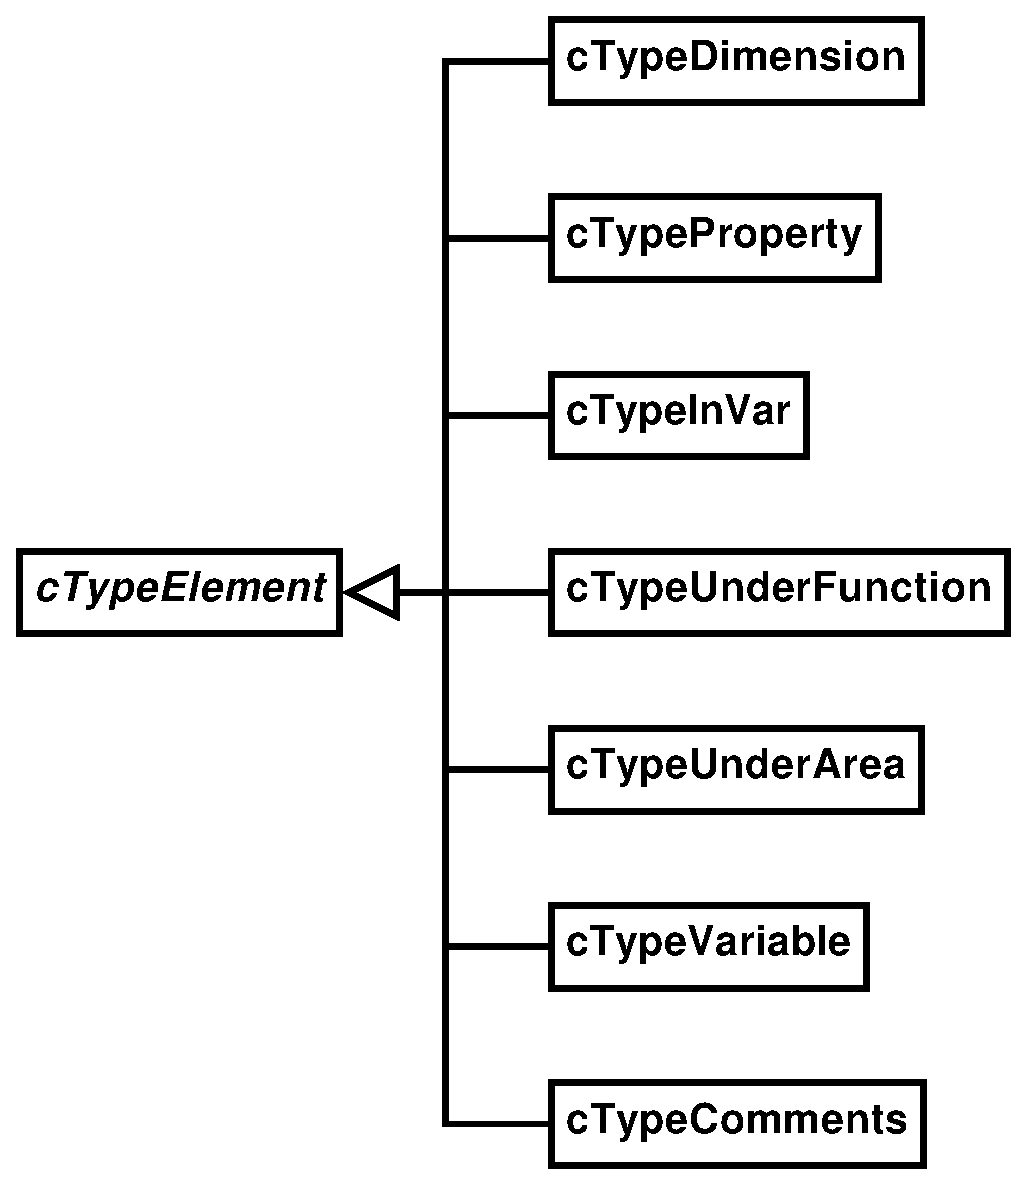
\includegraphics[scale=0.4]{fib_element_typen}
\end{center}
\caption{Klassengraph Fib-Elementtypen}
\label{figClassFibElementtyps}
\end{figure}

\subsubsection{getType}\index{cTypeElement!getType()}\index{getType()}

\textbf{Syntax:} \verb|unsignedIntFib getType()|

\bigskip\noindent
Diese Methode gibt eine Nummer f"ur den Typ des Elements zur"uck.

\bigskip\noindent
Die Nummern f"ur die Typen sind:
\begin{itemize}
 \item 1 f"ur cTypeDimension
 \item 2 f"ur cTypeSubarea
 \item 3 f"ur cTypeUnderFunction
 \item 5 f"ur cTypeInVar
 \item 6 f"ur cTypeProperty
 \item 10 f"ur cTypeVariable
 \item 11 f"ur cTypeComments
 \item 12 f"ur cTypeExternObject
 \item 13 f"ur cTypeExtSubobject
 \item 14 cTypeFibSet
 \item 15 cTypeFibMatrix
 \item 16 cTypeExtObjectInput
\end{itemize}

\bigskip\noindent
\textbf{Eingabeparameter:} keine

\bigskip\noindent
\textbf{R"uckgabe:} Der Typ des Vektors.


\subsubsection{isCompatible}\index{cTypeElement!isCompatible()}\index{isCompatible()}

\textbf{Syntax:} \verb|bool isCompatible( const cDomain & domain )|

\bigskip\noindent
Diese Methode gibt zur"uck, ob der Elemententyp kompatibel zum angegebenen Definitionsbereiche \verb|domain| ist.

\bigskip\noindent
\textbf{Eingabeparameter:}
\begin{itemize}
 \item \verb|domain|: Eine Referenz auf den Definitionsbereich, welcher kompatibel zum Typ des Elements sein soll.
\end{itemize}

\bigskip\noindent
\textbf{R"uckgabe:} Es wird \verb|true| (=wahr) zur"uckgegeben, wenn der Definitionsbereich \verb|domain| kompatibel ist, sonst \verb|false| (=falsch).


\subsubsection{getStandardDomain}\index{cTypeElement!getStandardDomain()}\index{getStandardDomain()}

\textbf{Syntax:} \verb|cDomain * getStandardDomain()|

\bigskip\noindent
Diese Methode gibt einen Zeiger auf den Standarddefinitionsbereich des Elemententyps zur"uck.

Das Objekt zum Standarddefinitionsbereich wird nicht automatisch gel"oscht. Das L"oschen des Objekts sollte also nach der Verwendung sichergestellt werden.

\bigskip\noindent
\textbf{Eingabeparameter:} keine

\bigskip\noindent
\textbf{R"uckgabe:} Zur"uckgegeben wird ein Zeiger auf den Standarddefinitionsbereich des Elemententyps.


\subsubsection{equalElementType}\index{cTypeElement!equalElementType()}\index{equalElementType()}

\textbf{Syntax:} \verb|bool equalElementType(| \\\verb| const cTypeElement & typeElement ) const|

\bigskip\noindent
Diese Methode pr"uft, ob der "ubergebene Elementtyp f"ur \verb|typeElement| mit dem aktuellen Elementtyp "ubereinstimmt. Zwei Elementtype stimmen "uberein, wenn sie zum gleichen Element geh"oren. Demnach darf es keine zwei Definitionsbereich zum gleichen Elementtyp gleichzeitig geben.

Der ein Positionselementtyp ist beispielsweise zu allen anderen m"oglichen Positionselementtypen gleich, unabh"angig von deren Dimension und Dimensionsmapping, da es nur eine Art von Positionsvektoren geben darf. Es gibt aber viele verschiedene Elementtypen f"ur die Eigenschaftstypen, da es f"ur verscheidene Eigenschaften verschiedene Vektoren geben kann.

\bigskip\noindent
\textbf{Eingabeparameter:}
\begin{itemize}
 \item \verb|typeElement|: Der Elementtyp, zu mit dem aktuelle Elementtyp "ubereinstimmt soll.
\end{itemize}

\bigskip\noindent
\textbf{R"uckgabe:} Wenn der aktuelle Elementtyp mit dem "ubergebenen \verb|typeElement| Elementtyp "ubereinstimmt, wird \verb|true| (=wahr) zur"uckgegeben, sonst wird \verb|false| (=falsch) zur"uckgegeben.


\subsubsection{equal}\index{cTypeElement!equal()}\index{equal()}

\textbf{Syntax:} \verb|bool equal( const cTypeElement & typeElement)const|

\noindent
\textbf{Syntax:} \verb|bool operator==( const cTypeElement & typeElement| \\\verb| ) const|

\bigskip\noindent
Diese Methode pr"uft, ob der "ubergebene Elementtyp \verb|typeElement| gleich zum aktuellen Elementtyp ist.

\bigskip\noindent
\textbf{Eingabeparameter:}
\begin{itemize}
 \item \verb|typeElement|: Der Elementtyp, zu dem der aktuelle Elementtyp gleich sein soll.
\end{itemize}

\bigskip\noindent
\textbf{R"uckgabe:} Wenn der aktuelle Elementtyp zum Elementtyp \verb|typeElement| gleich ist, wird \verb|true| (=wahr) zur"uckgegeben, sonst \verb|false| (=falsch).



\subsubsection{cTypeDimension}\index{cTypeElement!cTypeDimension}\index{cTypeDimension}

\textbf{Typ f"ur Element:} cVectorPosition; Die Nummer f"ur die Richtungen der Dimension werden "uber den Konstruktor bestimmt.

\bigskip\noindent
\textbf{Standarddefinitionsbereich:}

$vector( 2 , naturalNumberB(16), naturalNumberB(16) )$

\bigskip\noindent
\textbf{Kompatible Definitionsbereiche:} Vektoren

\bigskip\noindent
\textbf{Inkompatible Definitionsbereiche:} alle einzelnen Zahlen


\paragraph{Konstanten}

Folgende Konstanten werden von der Klasse \verb|cTypeDimension| definiert.

\begin{itemize}
 \item \verb|static const unsignedIntFib DIRECTION_NONE  = 0|
 \item \verb|static const unsignedIntFib DIRECTION_HORIZONTAL=1|
 \item \verb|static const unsignedIntFib DIRECTION_VERTICAL=2|
 \item \verb|static const unsignedIntFib DIRECTION_DEPTH = 3|
 \item \verb|static const unsignedIntFib DIRECTION_TIME  = 4|
\end{itemize}


\paragraph{cTypeDimension}

\ \\\\\noindent
\textbf{Syntax:} \verb|cTypeDimension(| \\\verb| unsigendIntFib iNumberOfDimensions=2 )|

\bigskip\noindent
Der Konstruktor des Dimensionstypobjekts, er erstellt einen Dimensionstypobjekt.

Den Dimensionen werden Initial die Werte 1 bis \verb|iNumberOfDimensions| zugeordnet, wie sie in Tabelle \ref{tableDimmapValues} auf Seite \pageref{tableDimmapValues} aufgef"uhrt sind. Bei zwei Dimensionen (Standardwert) w"are nach dem Erzeugen des Multimediainformationenobjekts die erste Dimension in Richtung ``horizontal'' und die zweite in Richtung ``vertikal''.

\bigskip\noindent
\textbf{Eingabeparameter:}
\begin{itemize}
 \item \verb|iNumberOfDimensions|: Die Anzahl der Dimensionen, welches das Fib-Objekt haben soll. Standardwert ist $2$ .
\end{itemize}

\bigskip\noindent
\textbf{R"uckgabe:} keine


\paragraph{cTypeDimension}

\ \\\\\noindent
\textbf{Syntax:} \verb|cTypeDimension(| \\\verb| vector<unsigendIntFib> vecDimensionsMapping )|

\bigskip\noindent
Der Konstruktor des Dimensionstypobjekts, er erstellt einen Dimensionstypobjekt.

\bigskip\noindent
\textbf{Eingabeparameter:}
\begin{itemize}
 \item \verb|vecDimensionsMapping|: Der Vektor mit den Mappingwerten f"ur die Dimensionen. Die Werte werden in Tabelle \ref{tableDimmapValues} auf Seite \pageref{tableDimmapValues} definiert. Der $i$'te Vektorwert steht f"ur die $i+1$'te Dimension. "Uber diesen Vektor wird auch die Anzahl der Dimensionen bestimmt. Wiederholt auftauchende Mappingwerte werden auf den Mappingwert $0$ f"ur ``none'' gesetzt.
\end{itemize}

\bigskip\noindent
\textbf{R"uckgabe:} keine


\paragraph{getNumberOfDimensions}\index{cTypeDimension!getNumberOfDimensions()}\index{getNumberOfDimensions()}

\ \\\\\noindent
\textbf{Syntax:} \verb|unsigendIntFib getNumberOfDimensions() const|

\bigskip\noindent
Diese Methode gibt die Anzahl der Dimensionen zur"uck, f"ur welche das Objekt steht.

\bigskip\noindent
\textbf{Eingabeparameter:} keine

\bigskip\noindent
\textbf{R"uckgabe:} Die Anzahl der Dimension, f"ur welche das Objekt steht.


\paragraph{getDimensionMapping}\index{cTypeDimension!getDimensionMapping()}\index{getDimensionMapping()}

\ \\\\\noindent
\textbf{Syntax:} \verb|unsignedIntFib getDimensionMapping(| \\\verb| unsignedIntFib iDimensionNumber ) const|

\bigskip\noindent
Diese Methode gibt den Mappingwert f"ur die Dimension \verb|iDimensionNumber| zur"uck. Existiert keine solche Dimension, wird $0$ f"ur \verb|none| zur"uckgegeben.

Die Werte werden in Tabelle \ref{tableDimmapValues} auf Seite \pageref{tableDimmapValues} definiert.

\bigskip\noindent
\textbf{Eingabeparameter:}
\begin{itemize}
 \item \verb|iDimensionNumber|: Nummer der Dimension, f"ur welche der Mappingwert zur"uckgegeben werden soll.
\end{itemize}

\bigskip\noindent
\textbf{R"uckgabe:} Den Mappingwert f"ur die Dimension \verb|iDimensionNumber|, existiert keine solche Dimension wird $0$ zur"uckgegeben.


\paragraph{setDimensionMapping}\index{cTypeDimension!setDimensionMapping()}\index{setDimensionMapping()}

\ \\\\\noindent
\textbf{Syntax:} \verb|bool setDimensionMapping(| \\\verb| unsignedIntFib iDimensionNumber,| \\\verb| unsignedLongFib lMapping )|

\bigskip\noindent
Diese Methode setzt den Mappingwert f"ur die Dimension \verb|iDimensionNumber|.
Die Werte werden in Tabelle \ref{tableDimmapValues} auf Seite \pageref{tableDimmapValues} definiert.

Wird versucht ein Mapping einzustellen, auf welches schon ein anderen Dimension gesetzt ist, wird das Mapping nicht ge"andert und \verb|false| (=falsch) zur"uckgegeben. Jede Dimension kann allerdings immer auf 0 (=kein Mapping) gesetzt werden.

Wenn kein entsprechendes \verb|iDimensionNumber|'tes Dimensionsmapping ex\-is\-tiert, wird \verb|false| (=falsch) zur"uckgegeben.

\bigskip\noindent
\textbf{Eingabeparameter:}
\begin{itemize}
 \item \verb|iDimensionNumber|: Nummer der Dimension, f"ur welche das Mapping ge"andert werden soll.
 \item \verb|lMapping|: Neuer Wert f"ur das Mapping der Dimension.
\end{itemize}

\bigskip\noindent
\textbf{R"uckgabe:} Es wird \verb|true| (=wahr) zur"uckgegeben, wenn das Mappingwert gesetzt wurden, sonst \verb|false| (=falsch).


\paragraph{getDimensionMappingName}\index{cTypeDimension!getDimensionMappingName()}\index{getDimensionMappingName()}

\ \\\\\noindent
\textbf{Syntax:} \verb|static string getDimensionMappingName(| \\\verb| unsignedLongFib ulMapping )|

\bigskip\noindent
Diese Methode liefert Namen f"ur den den Mappingwert \verb|ulMapping|.
Die Werte und Namen werden in Tabelle \ref{tableDimmapValues} auf Seite \pageref{tableDimmapValues} definiert und einander zugeordnet.


\bigskip\noindent
\textbf{Eingabeparameter:}
\begin{itemize}
 \item \verb|ulMapping|: Der Wert f"ur das Mapping, f"ur welche der Name zur"uckgegeben werden soll.
\end{itemize}

\bigskip\noindent
\textbf{R"uckgabe:} Den Namen f"ur den Mappingwert \verb|ulMapping|.


\paragraph{getUnit}\index{cTypeDimension!getUnit()}\index{getUnit()}

\ \\\\\noindent
\textbf{Syntax:} \verb| vector<string> getUnit() const|

\bigskip\noindent
Diese Methode gibt einen Vektor mit den Zeichenketten mit den (SI-) Einheiten f"ur die Vektorelemente/Dimensionen des Typs zur"uck.

Ist eine Einheit unbekannt (bzw. die Eigenschaft ist kein Standardtyp), wird eine leere Zeichenkette f"ur sie zur"uckgegeben.

\bigskip\noindent
\textbf{Eingabeparameter:} keine

\bigskip\noindent
\textbf{R"uckgabe:} Einen Vektor mit den Zeichenketten mit den (SI-) Einheiten f"ur die Vektorelemente des Typ.



\subsubsection{cTypeArea}\index{cTypeElement!cTypeArea}\index{cTypeArea}

\textbf{Typ f"ur Element:} cArea%; Die obere und untere Grenze f"ur die Unterbereiche.

\bigskip\noindent
\textbf{Standarddefinitionsbereich:} $vector( 2, naturalNumberB(8),$ $vector( 2,$ $integerB(16),$ $integerB(16) ) )$


Dieser Typ ist f"ur Definitionsbereich f"ur das Bereichselement (siehe Abschnitt \ref{fibArea} auf Seite \pageref{fibArea} und Abschnitt \ref{secCompressedArea} auf Seite \pageref{secCompressedArea}) im Haupt-Fib-Objekt. Der zugeh"orige Definitionsbereich ist ein Vektordefinitionsbereich mit 2 Elementen /Unterdefinitionsbereichen. Das erste Element bzw. der erste Unterdefinitionsbereich dient f"ur die Anzahl ($n$) der Unterbereiche, er ist ein Definitionsbereich aus den nat"urlichen Zahlen. Das zweite und letzte Element ist der Definitionsbereich f"ur die Vektoren f"ur die Unterbereiche ($B_{1}$) und ist ein Definitionsbereich f"ur Vektoren dessen zwei Elemente ganze Zahlen sind. 

\bigskip\noindent
\textbf{Kompatible Definitionsbereiche:} alle Vektoren mit zwei Elementen, deren erstes Element nat"urliche Zahlen ist und deren zweites Element ein Vektor mit zwei ganzen Zahlen ist

\bigskip\noindent
\textbf{Inkompatible Definitionsbereiche:} alle einzelnen Zahlen, alle Vektoren mit nicht zwei Unterdefinitionsbereichen und Vektoren in denen das erstes Element keine nat"urliche Zahlen ist oder der zweite Unterdefinitionsbereich kein Vektor mit zwei ganzen Zahlen ist


\subsubsection{cTypeUnderFunction}\index{cTypeElement!cTypeUnderFunction}\index{cTypeUnderFunction}

\textbf{Typ f"ur Element:} cUnderFunction; Die Zahlen in Funktionen.

\bigskip\noindent
\textbf{Standarddefinitionsbereich:} $naturalNumberB(16)$

\bigskip\noindent
\textbf{Kompatible Definitionsbereiche:} alle einzelnen Zahlen

\bigskip\noindent
\textbf{Inkompatible Definitionsbereiche:} Vektoren


\subsubsection{cTypeInVar}\index{cTypeElement!cTypeInVar}\index{cTypeInVar}

\textbf{Typ f"ur Element:} Eingabevariable $inVar_i$; Die Nummer der Eingabevariable wird "uber den Konstruktor bestimmt. Nur Eingabevariablen des aktuellen root-Elements k"onnen hier auftauchen.

\bigskip\noindent
\textbf{Standarddefinitionsbereich:} $naturalNumberB(16)$

\bigskip\noindent
\textbf{Kompatible Definitionsbereiche:} alle einzelnen Zahlen

\bigskip\noindent
\textbf{Inkompatible Definitionsbereiche:} Vektoren


\paragraph{cTypeInVar}

\ \\\\\noindent
\textbf{Syntax:} \verb|cTypeInVar( unsignedIntFib iNumberInputVariable )|

\bigskip\noindent
Der Konstruktor des Eingabevariablentypobjekts, er erstellt einen Eingabevariablentypobjekt.

\bigskip\noindent
\textbf{Eingabeparameter:}
\begin{itemize}
 \item \verb|iNumberInputVariable|: Die Nummer der Eingabevariable, f"ur welche das Objekt steht.
\end{itemize}

\bigskip\noindent
\textbf{R"uckgabe:} keine


\paragraph{getNumberOfInputVariable}\index{cTypeInVar!getNumberOfInputVariable()}\index{getNumberOfInputVariable()}

\ \\\\\noindent
\textbf{Syntax:} \verb|unsignedIntFib getNumberOfInputVariable() const|

\bigskip\noindent
Diese Methode gibt die Nummer der Eingabevariable zur"uck, f"ur das das Objekt steht.

\bigskip\noindent
\textbf{Eingabeparameter:} keine

\bigskip\noindent
\textbf{R"uckgabe:} Die Nummer der Eingabevariable, f"ur welche das Objekt steht.



\subsubsection{cTypeProperty}\index{cTypeElement!cTypeProperty}\index{cTypeProperty}

\textbf{Typ f"ur Element:} cVectorProperty; Der Typ der Eigenschaft wird "uber den Konstruktor bestimmt.

\bigskip\noindent
\textbf{Standarddefinitionsbereich:} $vector( 1 , naturalNumberB(16) )$

F"ur einige Eigenschaften ist der Standarddefinitionsbereich des Eigenschaftsvektors von $vector( 1 , naturalNumberB(16) )$ abweichend. In Tabelle \ref{tableElementsForDomains} auf Seite \pageref{tableElementsForDomains} sind die abweichenden Standarddefinitionsbereiche aufgef"uhrt.

\bigskip\noindent
\textbf{Kompatible Definitionsbereiche:} Vektoren deren Elemente einzelnen Zahlen sind

\bigskip\noindent
\textbf{Inkompatible Definitionsbereiche:} alle einzelnen Zahlen


\paragraph{Konstanten}

Folgende Konstanten werden von der Klasse \verb|cTypeProperty| definiert:

\begin{itemize}
 \item \verb|static const unsignedIntFib COLOR_RGB = 1|
 \item \verb|static const unsignedIntFib COLOR_GRAYSCALE  = 2|
 \item \verb|static const unsignedIntFib LAYER     = 100|
 \item \verb|static const unsignedIntFib TRANSPARENCY    = 200|
 \item \verb|static const unsignedIntFib SOUND     = 300|
 \item \verb|static const unsignedIntFib SOUND_POLARIZED = 301|
 \item \verb|static const unsignedIntFib SOUND_AMPLITUDE = 305|
 \item \verb|static const unsignedIntFib SOUND_BARRIER   = 310|
 \item \verb|static const unsignedIntFib SOUND_REFLECTED = 311|
 \item \verb|static const unsignedIntFib SOUND_DAMPING   = 312|
 \item \verb|static const unsignedIntFib KELVIN    = 400|
 \item \verb|static const unsignedIntFib ELECTRO_MAGNETIC= 410|
\end{itemize}


\paragraph{cTypeProperty}\index{cTypeElement!cTypeProperty}

\ \\\\\noindent
\textbf{Syntax:} \verb|cTypeProperty( intFib iTypeProperty )|

\bigskip\noindent
Der Konstruktor des Eigenschaftstypobjekts, er erstellt einen Eigenschaftstypobjekt.

Die Nummer des Eigenschaftstyps sind die Werte aus Tabelle \ref{tablePropertyNamen} auf Seite \pageref{tablePropertyNamen} .

\bigskip\noindent
\textbf{Eingabeparameter:}
\begin{itemize}
 \item \verb|iTypeProperty|: Die Nummer des Typs, der Eigenschaft f"ur das das Objekt steht. Die m"oglichen Werte f"ur die unterschiedlichen Eigenschaften sind aus Tabelle \ref{tablePropertyNamen} auf Seite \pageref{tablePropertyNamen} aus der Spalte ``Wert'' zu entnehmen.
\end{itemize}

\bigskip\noindent
\textbf{R"uckgabe:} keine


\paragraph{cTypeProperty}

\ \\\\\noindent
\textbf{Syntax:} \verb|cTypeProperty( unsignedIntFib uiPropertyType,| \\\verb| unsignedIntFib uiNumberOfDimensions=2 )|

\bigskip\noindent
Der Konstruktor des Eigenschaftstypobjekts, er erstellt einen Eigenschaftstypobjekts.

\bigskip\noindent
\textbf{Eingabeparameter:}
\begin{itemize}
 \item \verb|uiPropertyType|: Die Nummer der Eigenschaft, f"ur welche das Objekt steht.
 \item \verb|uiNumberOfDimensions|: Die Nummer der der Dimensionen der Eigenschaft. Bei manche Eigenschaften ist die Anzahl der Element von der Dimension abh"angig (z.B $soundPolarized$), deshalb wird diee Angabe ben"otigt.
\end{itemize}

\bigskip\noindent
\textbf{R"uckgabe:} keine


\paragraph{getNumberOfProperty}\index{cTypeProperty!getNumberOfProperty()}\index{getNumberOfProperty()}

\ \\\\\noindent
\textbf{Syntax:} \verb|unsignedIntFib getNumberOfProperty()|

\bigskip\noindent
Diese Methode gibt die Nummer der Eigenschaft zur"uck, f"ur welche das Objekt steht.
In Tabelle \ref{tablePropertyNamen} auf Seite \pageref{tablePropertyNamen} sind die Nummern der Eigenschaften ind der Spalte ``Wert'' aufgef"uhrt.

\bigskip\noindent
\textbf{Eingabeparameter:} keine

\bigskip\noindent
\textbf{R"uckgabe:} Die Nummer der Eigenschaft f"ur das das Objekt steht.


\paragraph{getNumberOfProperty}\index{cTypeProperty!getNumberOfProperty()}\index{getNumberOfTypeProperty()}

\ \\\\\noindent
\textbf{Syntax:} \verb|intFib getNumberOfTypeProperty() const|

\bigskip\noindent
Diese Methode gibt die Nummer des Typs der Eigenschaft zur"uck, f"ur welchen das Objekt steht.

Die Nummer des Eigenschaftstyps sind die Werte aus Tabelle \ref{tablePropertyNamen} auf Seite \pageref{tablePropertyNamen} in der Spalte ``Wert'' aufgef"uhrt.

\bigskip\noindent
\textbf{Eingabeparameter:} keine

\bigskip\noindent
\textbf{R"uckgabe:} Die Nummer der des Typs der Eigenschaft, f"ur welche das Objekt steht.


\paragraph{getUnit}\index{cTypeProperty!getUnit()}\index{getUnit()}

\ \\\\\noindent
\textbf{Syntax:} \verb|vector<string> getUnit() const|

\bigskip\noindent
Diese Methode gibt einen Vektor mit den Zeichenketten mit den (SI-) Einheiten f"ur die Vektorelemente des Typs zur"uck.

Ist eine Einheit unbekannt (bzw. die Eigenschaft ist kein Standardtyp), wird eine leere Zeichenkette f"ur sie zur"uckgegeben.

\bigskip\noindent
\textbf{Eingabeparameter:} keine

\bigskip\noindent
\textbf{R"uckgabe:} Einen Vektor mit den Zeichenketten mit den (SI-) Einheiten f"ur die Vektorelemente des Eigenschaftstyps.



\subsubsection{cTypeVariable}\index{cTypeElement!cTypeVariable}\index{cTypeVariable}

\textbf{Typ f"ur Element:} cVariable

\bigskip\noindent
\textbf{Standarddefinitionsbereich:} $naturalNumberB(8)$

Der zugeh"orige Definitionsbereich dient f"ur die Werte die ben"otigt werden, um Variablen im komprimierten Speicherformat zu kodieren. Der Definitionsbereich sollten die nat"urliche Zahlen von 0 bis maximale Anzahl der definierten Variablen in den Fib-Bl"attern im Haupt-Fib-Objekt sein. Das Fib-Baum-Blatt im Haupt-Fib-Objekt "uber dem meisten Variablen definiert werden, bestimmt also den Definitionsbereich, bzw. der Ast mit den meisten definierten Variablen. Dieser Eintrag wird beim Abspeichern erstellt.

\bigskip\noindent
\textbf{Kompatible Definitionsbereiche:} alle nat"urlichen, unskalierte Zahlen

\bigskip\noindent
\textbf{Inkompatible Definitionsbereiche:} alle einzelnen Zahlen die nicht nat"urlichen, unskalierte Zahlen sind und alle Vektoren



\subsubsection{cTypeComments}\index{cTypeElement!cTypeComments}\index{cTypeComments}

\textbf{Typ f"ur Element:} cComment

\bigskip\noindent
\textbf{Standarddefinitionsbereich:} $naturalNumberB(8)$

Der zugeh"orige Definitionsbereich dient f"ur die Werte die ben"otigt werden, um Kommentare im komprimierten Speicherformat zu kodieren. Der Definitionsbereich sollten die nat"urliche Zahlen von 0 bis Anzahl der Kommentare im Haupt-Fib-Objekt sein. Dieser Eintrag wird beim Abspeichern erstellt.

\bigskip\noindent
\textbf{Kompatible Definitionsbereiche:} alle nat"urlichen, unskalierte Zahlen

\bigskip\noindent
\textbf{Inkompatible Definitionsbereiche:} alle einzelnen Zahlen die nicht nat"urlichen, unskalierte Zahlen sind und alle Vektoren


\subsubsection{cTypeExtObjekt}\index{cTypeElement!cTypeExtObjekt}\index{cTypeExtObjekt}

\textbf{Typ f"ur Element:} cExtObjekt

\bigskip\noindent
\textbf{Standarddefinitionsbereich:}

$vector( 4 , integerB(32), naturalNumberB(4), naturalNumberB(2),$

$naturalNumberB(2) )$

Dieser Typ ist f"ur Definitionsbereich f"ur externe Objekte im Haupt-Fib-Objekt. Der Definitionsbereich ist ein Vector mit 4 Elementen. Die Vektorelemente dienen der Reihenfolge f"ur den Identifier, die Anzahl der Eingabevariablen NumberInVar, die Anzahl der Unterobjekte NumberUnderObjects und die Anzahl der Ausgabevariablen NumberOutVar. Alle Vektorelementdefinitionsbereiche, au"ser dem f"ur den Identifier, kommen aus den nat"urlichen Zahlen. Der Vektorelementdefinitionsbereich f"ur den Identifier kommt aus den Ganzzahlen. Dieser Definitionsbereich wird normalerweise beim Abspeichern erstellt.

\bigskip\noindent
\textbf{Kompatible Definitionsbereiche:} Vektoren mit 4 Elementen deren erstes Elemente eine einzelnen Ganzzahlen ist und dessen anderen Elemente nat"urliche Zahlen sind, alle Vektorelemente sind unskaliert

\bigskip\noindent
\textbf{Inkompatible Definitionsbereiche:} alle einzelnen Zahlen, alle Vektoren die nicht kompatible sind


\subsubsection{cTypeExtObjectInput}\index{cTypeElement!cTypeExtObjectInput}\index{cTypeExtObjectInput}

\textbf{Typ f"ur Element:} Eingabewerte von externen Objekten (cExtObjekt); Der Identifier des externen Objekts wird "uber den Konstruktor bestimmt.

\bigskip\noindent
\textbf{Standarddefinitionsbereich:} $vectorOpenEnd( integerB(8) )$

\bigskip\noindent
\textbf{Kompatible Definitionsbereiche:} Vektoren deren Elemente einzelnen Zahlen sind

\bigskip\noindent
\textbf{Inkompatible Definitionsbereiche:} alle einzelnen Zahlen


\paragraph{cTypeExtObjectInput}

\ \\\\\noindent
\textbf{Syntax:} \verb|cTypeExtObjectInput( long lIdentifier )|

\bigskip\noindent
Der Konstruktor des Eingabewertetypobjekts f"ur externen Objekten, er erstellt einen Eingabewertetypobjekt f"ur externen Objekten mit dem Identifier lIdentifier.

\bigskip\noindent
\textbf{Eingabeparameter:}
\begin{itemize}
 \item \verb|lIdentifier|: Der Identifier des externen Objekts, f"ur welche das Objekt steht.
\end{itemize}

\bigskip\noindent
\textbf{R"uckgabe:} keine


\paragraph{getIdentifier}\index{cTypeExtObjectInput!getIdentifier()}\index{getIdentifier()}

\ \\\\\noindent
\textbf{Syntax:} \verb|long getIdentifier() const|

\bigskip\noindent
Diese Methode gibt den Identifier des externen Objekts zur"uck, f"ur dessen Eingabewerte das Objekt steht.

\bigskip\noindent
\textbf{Eingabeparameter:} keine

\bigskip\noindent
\textbf{R"uckgabe:} Die Identifier des externen Objekts, f"ur dessen Eingabewerte das Objekt steht.



\subsubsection{cTypeExtSubobject}\index{cTypeElement!cTypeExtSubobject}\index{cTypeExtSubobject}

\textbf{Typ f"ur Element:} f"ur das externe Subobjekt (cExtSubobject); Die Nummer des externen Subobjekts wird "uber den Konstruktor bestimmt. Nur externe Subobjekte des Haup-Fib-Objects des aktuellen root-Elements k"onnen hier auftauchen.

\bigskip\noindent
\textbf{Standarddefinitionsbereich:} $vector( 0 )$

\bigskip\noindent
\textbf{Kompatible Definitionsbereiche:} Vektoren deren Elemente einzelnen Zahlen sind

\bigskip\noindent
\textbf{Inkompatible Definitionsbereiche:} alle einzelnen Zahlen


\paragraph{cTypeExtSubobject}

\ \\\\\noindent
\textbf{Syntax:} \verb|cTypeExtSubobject( const unsignedIntFib iNumberExtSubobject )|

\bigskip\noindent
Der Konstruktor des externen Subobjekt Typs, er erstellt einen externe Subobjekt Type.

\bigskip\noindent
\textbf{Eingabeparameter:}
\begin{itemize}
 \item \verb|iNumberExtSubobject|: Die Nummer des externen Subobjekts, f"ur welche das Objekt steht.
\end{itemize}

\bigskip\noindent
\textbf{R"uckgabe:} keine


\paragraph{getNumberOfExtSubobject}\index{cTypeExtSubobject!getNumberOfExtSubobject()}\index{getNumberOfExtSubobject()}

\ \\\\\noindent
\textbf{Syntax:} \verb|unsignedIntFib getNumberOfExtSubobject() const|

\bigskip\noindent
Diese Methode gibt die Nummer des externen Subobjekts zur"uck, f"ur das das Objekt steht.

\bigskip\noindent
\textbf{Eingabeparameter:} keine

\bigskip\noindent
\textbf{R"uckgabe:} Die Nummer der externen Subobjekts, f"ur welche das Objekt steht.



% TODO weg:
% \subsubsection{cTypeExtSubobject}\index{cTypeElement!cTypeExtSubobject}\index{cTypeExtSubobject}
% 
% \textbf{Typ f"ur Element:} cExtSubobject
% 
% \bigskip\noindent
% \textbf{Standarddefinitionsbereich:} $naturalNumberB(4)$
% 
% Der zugeh"orige Definitionsbereich dient f"ur die Anzahl der Eingebevariablen f"ur externe Unterobjekte. Der Definitionsbereich ist immer eine Untermenge der nat"urlichen Zahlen und wird normalerweise beim Abspeichern erstellt.
% 
% \bigskip\noindent
% \textbf{Kompatible Definitionsbereiche:} alle nat"urlichen, unskalierte Zahlen
% 
% \bigskip\noindent
% \textbf{Inkompatible Definitionsbereiche:} alle einzelnen Zahlen die nicht nat"urlichen, unskalierte Zahlen sind und alle Vektoren




\subsubsection{cTypeFibSet}\index{cTypeElement!cTypeFibSet}\index{cTypeFibSet}

\textbf{Typ f"ur Element:} cTypeFibSet

\bigskip\noindent
\textbf{Standarddefinitionsbereich:} $vector( 3, naturalNumberB(8),$ $naturalNumberB(32),$ $vectorOpenEnd( 1,$ $integerB(32) ) )$

Dieser Typ ist f"ur Definitionsbereich f"ur das set-Element (siehe Abschnitt \ref{secFibSetElement} auf Seite \pageref{secFibSetElement} und Abschnitt \ref{secCFibSetElement} auf Seite \pageref{secCFibSetElement}) im Haupt-Fib-Objekt. Der Definitionsbereich ist ein Vector mit 3 Elementen.  Das erste Element bzw. der erste Unterdefinitionsbereich dient f"ur die Anzahl ($n$) der Variablen und der zu setzenden Werte pro Satz, er ist ein Definitionsbereich aus den nat"urlichen Zahlen. Das zweite Element bzw. der zweite Unterdefinitionsbereich dient f"ur die Anzahl ($k$) der S"atze mit zu setzenden Werten. Er ist auch ein Definitionsbereich aus den nat"urlichen Zahlen. Das dritte und letzte Element ist der Definitionsbereich f"ur die Vektoren f"ur die zu setzenden Werte ($W_{i.g}$) und ist ein Definitionsbereich f"ur Vektoren deren Elemente einfache Zahlen (skalare) sind.

\bigskip\noindent
\textbf{Kompatible Definitionsbereiche:} alle Vektoren mit drei Elementen, deren ersten beiden Elemente nat"urliche Zahlen sind und deren drittes Element ein beliebiger Vektor mit Zahlen ist

\bigskip\noindent
\textbf{Inkompatible Definitionsbereiche:} alle einzelnen Zahlen, alle Vektoren mit nicht drei Unterdefinitionsbereichen und Vektoren in denen die ersten beiden Elemente keine nat"urliche Zahlen sind oder der dritte Unterdefinitionsbereich kein Vektor von Zahlen ist


\subsubsection{cTypeFibMatrix}\index{cTypeElement!cTypeFibMatrix}\index{cTypeFibMatrix}

\textbf{Typ f"ur Element:} cTypeFibMatrix

\bigskip\noindent
\textbf{Standarddefinitionsbereich:} $vector( 4, naturalNumberB(8),$ $naturalNumberB(32),$ $vector( 2 , integerB(16), integerB(16) )$, $vectorOpenEnd( 1,$ $integerB(32) ) )$

Dieser Typ ist f"ur Definitionsbereich f"ur das Matrixelement (siehe Abschnitt \ref{secFibMatrixElement} auf Seite \pageref{secFibMatrixElement} und Abschnitt \ref{secCFibMatrixElement} auf Seite \pageref{secCFibMatrixElement}) im Haupt-Fib-Objekt. Der Definitionsbereich ist ein Vector mit 4 Elementen.  Das erste Element bzw. der erste Unterdefinitionsbereich ist f"ur die Anzahl ($d$) der Dimensionsvariablen, die Anzahl ($i$) der Wertevariablen und die zu setzenden Werte $i$ pro Satz. Er ist ein Definitionsbereich aus den nat"urlichen Zahlen. Das zweite Element bzw. der zweite Unterdefinitionsbereich ist f"ur die Anzahl ($k$) der S"atze mit den zu setzenden Werten. Er ist auch ein Definitionsbereich aus den nat"urlichen Zahlen. Das dritte Element ist der Definitionsbereich f"ur die Bereiche bzw. Start und Endwerte f"ur die einzellenen Dimensionsvariablen, er ist ein Vektordefinitionsbereich mit zwei Elementen, welche jeweils aus den ganzen Zahlen kommen. Das vierte und letzte Element ist der Definitionsbereich f"ur die Vektoren f"ur die zu setzenden Werte ($W_{a.b}$) und ist ein Definitionsbereich f"ur Vektoren deren Elemente einfache Zahlen (skalare) sind.

\bigskip\noindent
\textbf{Kompatible Definitionsbereiche:} alle Vektoren mit vier Elementen, deren ersten beiden Elemente nat"urliche Zahlen sind, deren drittes Element ein Vektor mit zwei Ganzzahlen und deren viertes Element ein beliebiger Vektor mit Zahlen ist

\bigskip\noindent
\textbf{Inkompatible Definitionsbereiche:} alle einzelnen Zahlen, alle Vektoren mit nicht vier Unterdefinitionsbereichen und Vektoren in denen die ersten beiden Elemente keine nat"urliche Zahlen sind, Vektoren in denen der dritte Unterdefinitionsbereich kein Vektor von zwei Ganzzahlen ist oder der vierte Unterdefinitionsbereich kein Vektor von Zahlen ist



\subsection{Definitionsbereiche cDomain}\index{root-Element!Definitionsbereiche}\index{cDomains!cDomain}\index{cDomain}

Definitionsbereiche dienen zur Eingrenzung der m"oglichen Werte, welche ein Element einnehmen kann.

Es gibt zwei gro"se Klassen von Definitionsbereichen: Vektoredefinitionsbereiche und Definitionsbereiche f"ur einzelne (skalare) Werte/ Zahlen.

In Diagramm \ref{figClassFibDomains} ist eine Klassenhierarchie der Definitionsbereiche dargestellt.

\begin{figure}[htbp]
\begin{center}
  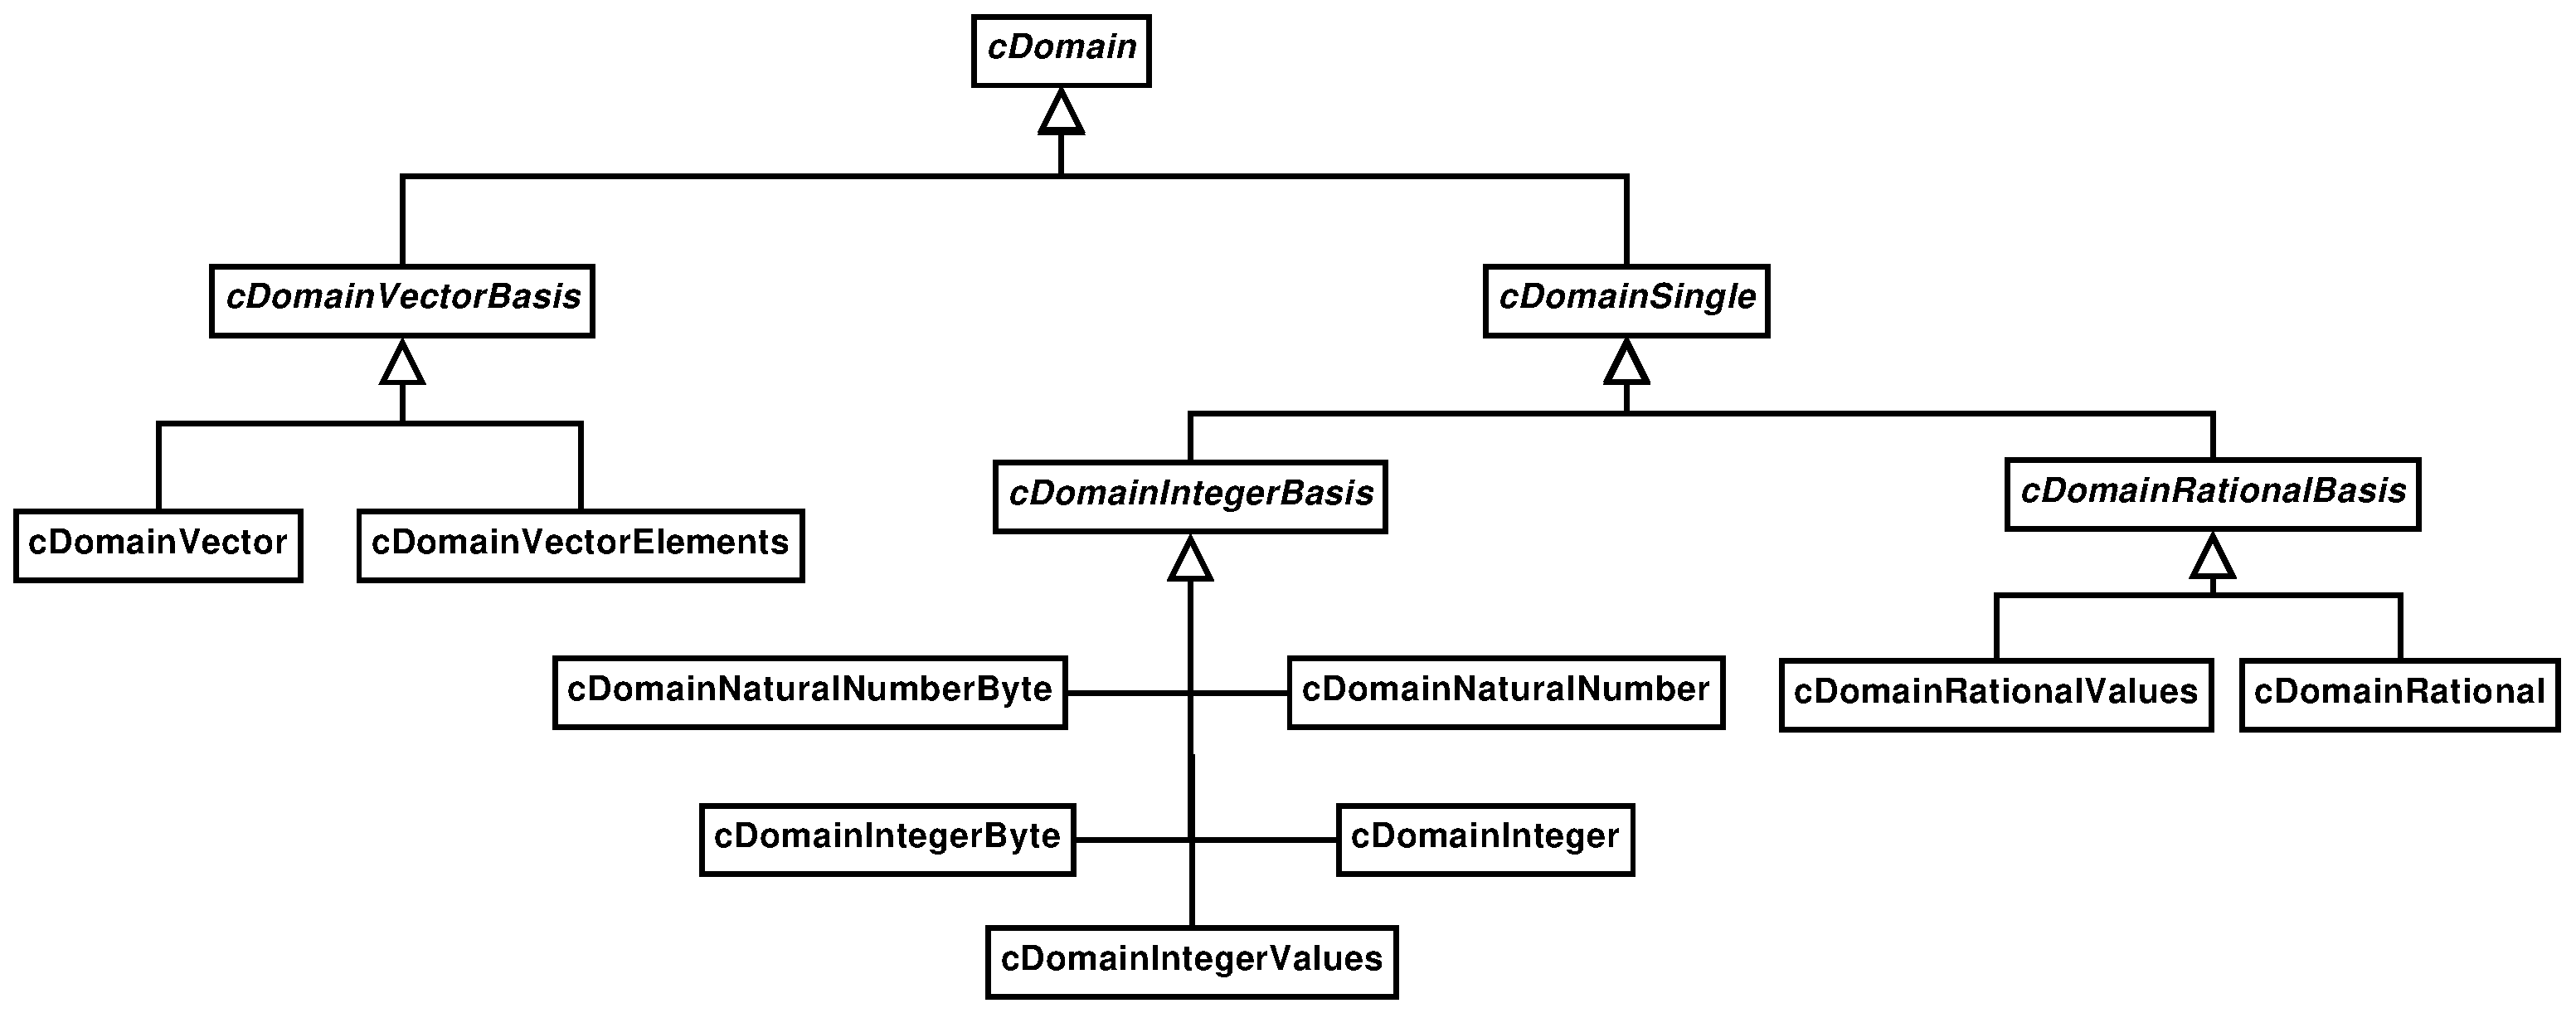
\includegraphics[scale=0.25]{fib_definition_areas}
\end{center}
\caption{Klassengraph der Fib-Definitionsbereiche}
\label{figClassFibDomains}
\end{figure}


\subsubsection{getType}\index{cDomain!getType()}\index{getType()}

\textbf{Syntax:} \verb|string getType()|

\bigskip\noindent
Diese Methode gibt den Typ des Definitionsbereichs als Zeichenkette zur"uck. Dies ist der Klassenname ohne das vorangestellte Zeichen ``c''. Beispielsweise geben Objekte der Klasse \verb|cDomainNaturalNumberBit| die Zeichenkette ``DomainNaturalNumberBit'' als Typ zur"uck.

\bigskip\noindent
\textbf{Eingabeparameter:} keine

\bigskip\noindent
\textbf{R"uckgabe:} Zur"uckgegeben wird der Typ des Definitionsbereichs als Zeichenkette.



\subsection{Einfache Definitionsbereiche cDomainSingle}\index{cDomain!cDomainSingle}\index{cDomainSingle}

Die Klasse \verb|cDomainSingle| ist der Basisklasseh aller einzelnen Zahlen (Skalare). Von \verb|cDomainSingle| werden alle Definitionsbereiche f"ur einfache Zahlen abgeleitet. Von \verb|cDomainSingle| selbst kann jedoch keine Instanz erzeugt werden.

Nach den folgenden Methoden der Klasse \verb|cDomainSingle| sind die von ihr abgeleiteten Klassen aufgef"uhrt.


\subsubsection{isElement}\index{cDomainSingle!isElement()}\index{isElement()}

\textbf{Syntax:} \verb|bool isElement( const doubleFib dValue ) const|

\bigskip\noindent
Diese Methode pr"uft, ob der "ubergebene Wert \verb|dValue| im (skalierten) Definitionsbereich liegt.

Diese Methode ist mit Vorsicht zu verwenden, da aufgrund von Rundungsfehlern bei Gleitkommawerten (\verb|doubleFib|) diese leicht voneinander abweichen k"onnen. F"ur Werte die von der \verb|round()| Methode zur"uckgegeben werden, gibt die \verb|isElement()| Methode \verb|true| (=wahr) zur"uck. Wenn aber beispielsweise zum R"uckgabewert $W$ der \verb|round()| Methode $3$ addiert und wieder abgezogen wird ($W+3-3$), ist das Ergebnis der \verb|isElement()| Methode unbestimmt.

\bigskip\noindent
\textbf{Eingabeparameter:}
\begin{itemize}
 \item \verb|dValue|: Der Wert, f"ur den zu pr"ufen ist, ob er im Definitionsbereich liegt.
\end{itemize}

\bigskip\noindent
\textbf{R"uckgabe:} Wenn der "ubergebene Wert \verb|dValue| im Definitionsbereich liegt, wird \verb|true| (=wahr) zur"uckgegeben, sonst \verb|false| (=falsch).


\subsubsection{round}\index{cDomainSingle!round()}\index{round()}

\textbf{Syntax:} \verb|doubleFib round( const doubleFib dValue ) const|

\bigskip\noindent
Diese Methode rundet den "ubergebenen Wert \verb|dValue| auf einen Wert, der im (skalierten) Definitionsbereich liegt und den minimalen Abstand zum "ubergebenen Wert \verb|dValue| hat. Gibt es mehrere Werte mit minimalen Abstand zum Wert \verb|dValue|, wird der kleinste genommen.

\bigskip\noindent
\textbf{Eingabeparameter:}
\begin{itemize}
 \item \verb|dValue|: Der Wert, der auf einen Wert im Definitionsbereich zu runden ist.
\end{itemize}

\bigskip\noindent
\textbf{R"uckgabe:} Ein Wert der im (skalierten) Definitionsbereich liegt und dem "ubergebenen Wert \verb|lValue| m"oglichst nahe kommt.


\subsubsection{getMaximum}\index{cDomainSingle!getMaximum()}\index{getMaximum()}

\textbf{Syntax:} \verb|doubleFib getMaximum() const|

\bigskip\noindent
Diese Methode liefert den gr"o"sten Wert des (skalierten) Definitionsbereichs.

\bigskip\noindent
\textbf{Eingabeparameter:} keine

\bigskip\noindent
\textbf{R"uckgabe:} Zur"uckgegeben wird der gr"o"ste Wert des Definitionsbereichs.


\subsubsection{getMinimum}\index{cDomainSingle!getMinimum()}\index{getMinimum()}

\textbf{Syntax:} \verb|doubleFib getMinimum() const|

\bigskip\noindent
Diese Methode liefert den kleinsten Wert des (skalierten) Definitionsbereichs.

\bigskip\noindent
\textbf{Eingabeparameter:} keine

\bigskip\noindent
\textbf{R"uckgabe:} Zur"uckgegeben wird der kleinste Wert des Definitionsbereichs.


\subsubsection{getNull}\index{cDomainSingle!getNull()}\index{getNull()}

\textbf{Syntax:} \verb|doubleFib getNull() const|

\bigskip\noindent
Diese Methode liefert den Nullwert des (skalierten) Definitionsbereichs.

Der Nullwert ist der Wert der entsteht, wenn die Zahl $0$ auf einen Wert im Definitionsbereich gerundet wird.

Der Nullwert wird beispielsweise verwendet, wenn eine Eingabevariable nicht belegt wurde.

\bigskip\noindent
\textbf{Eingabeparameter:} keine

\bigskip\noindent
\textbf{R"uckgabe:} Zur"uckgegeben wird der Nullwert des Definitionsbereichs.



\subsubsection{cDomainIntegerBasis}\index{cDomain!cDomainIntegerBasis}

Die Klasse \verb|cDomainIntegerBasis| ist die Basisklasse der Definitionsbereiche f"ur skalierte ganze Zahlen. Von dieser Klasse \verb|cDomainIntegerBasis| werden alle Definitionsbereiche f"ur skalierte ganze Zahlen abgeleitet. Von der Klasse \verb|cDomainIntegerBasis| selbst kann jedoch keine Instanz erzeugt werden.

Zahlen aus diesem Definitionsbereich sind Zahlen, die mit einem Skalierungsfaktor $S$ skaliert werden. DEr Skalierungsfaktor mu"s immer gr"o"ser als $0$ sein. Standardwert f"ur den Skalierungsfaktor $S$ ist $1$, wodurch die Werte des Definitionsbereichs nicht skaliert werden. Die Skalierung dient dazu, um (ganze) Zahlen besser auf die SI-Einheiten Mappen zu k"onnen. Er kann ignoriert werden, wenn z. B. das Anzeigeger"at zu klein oder viel zu gro"s ist, f"ur eine vollst"andige Anzeige aller Werte des Definitionsbereichs. Beispielsweise wenn der Definitionsbereich f"ur die horizontale Dimension von 0 m bis 10 m (Meter) geht, aber der Monitor nur 30 cm Breit ist.

F"ur die von \verb|cDomainIntegerBasis| abgeleiteten Klassen gibt zwei Gruppen von Methoden, eine, welche die Werte ohne Skalierung zur"uckgibt, und eine, welche die Werte skaliert zur"uckgibt. Die Funktionen, welche auf nicht skalierten Werten arbeiten, haben ``Unscaled'' in ihrem Namen. Sind im Definitionsbereich nur Ganzzahlen (z. B. bei Unterbereichen) ist es besser die ``Unscaled'' Methoden zu verwenden. Im allgemeinen sind Werte der Methoden bzw. ihre R"uckgabe auf dem skalierten Definitionsbereich nicht kompatibel zu ihren ``Unscaled'' Methoden. Gibt beispielsweise die \verb|isElement()| Methode f"ur einen Wert \verb|true| zur"uck, ist die R"uckgabe von \verb|isUnscaledElement()| nicht unbedingt auch \verb|true| , selbst wenn der Skalierungsfaktor $1$ ist.

Die skalierte Ganzzahlen sind von Gleitkommazahlen zu unterscheiden. Bei skalierte Ganzzahlen haben die einzelnen Werte immer einen Abstand der ein vielfaches des Skalierungsfaktors $S$ ist, dies gilt nicht f"ur Gleitkommazahlen. Skalierte Ganzzahlen sind in gewisser Weise Ganzzahlen mit einer anderen Einheit, welche sich aus der urspr"unglichen SI-Einheit durch Multiplikation mit dem Skalierungsfaktor $S$ ergibt.


\paragraph{getScalingFactor}\index{cDomainIntegerBasis!getScalingFactor()}\index{getScalingFactor()}

\ \\\\\noindent
\textbf{Syntax:} \verb|doubleFib getScalingFactor() const|

\bigskip\noindent
Diese Methode gibt den Skalierungsfaktor des Definitionsbereichs zur"uck.

\bigskip\noindent
\textbf{Eingabeparameter:} keine

\bigskip\noindent
\textbf{R"uckgabe:} Den Skalierungsfaktor des Definitionsbereichs.


\paragraph{scale}\index{cDomainIntegerBasis!scale()}\index{scale()}

\ \\\\\noindent
\textbf{Syntax:} \verb|doubleFib scale( const longFib lValue ) const|

\bigskip\noindent
Diese Methode skaliert den "ubergebenen Wert \verb|lValue| auf einen Wert der im skalierten Definitionsbereich liegt und den minimalen Abstand zum skalierten Wert ($lValue * S$) des "ubergebenen Wert \verb|lValue| hat. Gibt es mehrere skalierte Werte mit minimalen Abstand zum skalierten Wert von \verb|lValue| , wird der kleinste genommen.

\bigskip\noindent
Beispiele f"ur ein Definitionsbereich mit den nat"urlichen unskalierten Zahlen von $0$ bis $4$ und den Skalierungsfaktor $S$ von 5:
\begin{itemize}
 \item $scale( -2 ) = 0$
 \item $scale( 0 ) = 0$
 \item $scale( 1 ) = 5$
 \item $scale( 2 ) = 10$
 \item $scale( 4 ) = 20$
 \item $scale( 10 ) = 20$
\end{itemize}


\bigskip\noindent
\textbf{Eingabeparameter:}
\begin{itemize}
 \item \verb|lValue|: Der Wert, welcher zu skalieren ist.
\end{itemize}

\bigskip\noindent
\textbf{R"uckgabe:} Ein Wert der im skalierten Definitionsbereich liegt und dem skalierten Wert des "ubergebenen Werts \verb|lValue| m"oglichst nahe kommt.


\paragraph{isUnscaledElement}\index{cDomainIntegerBasis!isUnscaledElement()}\index{isUnscaledElement()}

\ \\\\\noindent
\textbf{Syntax:} \verb|bool isUnscaledElement(| \\\verb| const longFib lValue ) const|

\bigskip\noindent
Diese Methode pr"uft, ob der "ubergebene Wert \verb|lValue| im unskalierten Definitionsbereich liegt.

\bigskip\noindent
\textbf{Eingabeparameter:}
\begin{itemize}
 \item \verb|lValue|: Der Wert, f"ur den zu pr"ufen ist, ob er im unskalierten Definitionsbereich liegt.
\end{itemize}

\bigskip\noindent
\textbf{R"uckgabe:} Wenn der "ubergebene Wert \verb|lValue| im unskalierten Definitionsbereich liegt, wird \verb|true| (=wahr) zur"uckgegeben, sonst \verb|false| (=falsch).


\paragraph{roundUnscaled}\index{cDomainIntegerBasis!roundUnscaled()}\index{roundUnscaled()}

\ \\\\\noindent
\textbf{Syntax:} \verb|longFib roundUnscaled(| \\\verb| const longFib lValue ) const|

\bigskip\noindent
Diese Methode rundet den "ubergebenen Wert \verb|lValue| auf einen Wert der im unskalierten Definitionsbereich liegt und den minimalen Abstand zum "ubergebenen Wert \verb|lValue| hat. Gibt es mehrere Werte mit minimalen Abstand zum Wert \verb|lValue| wird der kleinste genommen.

\bigskip\noindent
\textbf{Eingabeparameter:}
\begin{itemize}
 \item \verb|lValue|: Der Wert, welcher auf einen Wert im unskalierten Definitionsbereich zu runden ist.
\end{itemize}

\bigskip\noindent
\textbf{R"uckgabe:} Ein Wert der im unskalierten Definitionsbereich liegt und dem "ubergebenen Wert \verb|lValue| m"oglichst nahe kommt.


\paragraph{getMaximumUnscaled}\index{cDomainIntegerBasis!getMaximumUnscaled()}\index{getMaximumUnscaled()}

\ \\\\\noindent
\textbf{Syntax:} \verb|longFib getMaximumUnscaled() const|

\bigskip\noindent
Diese Methode liefert den gr"o"sten Wert des unskalierten Definitionsbereichs.

\bigskip\noindent
\textbf{Eingabeparameter:} keine

\bigskip\noindent
\textbf{R"uckgabe:} Zur"uckgegeben wird der gr"o"ste Wert des unskalierten Definitionsbereichs.


\paragraph{getMinimumUnscaled}\index{cDomainIntegerBasis!getMinimumUnscaled()}\index{getMinimumUnscaled()}

\ \\\\\noindent
\textbf{Syntax:} \verb|longFib getMinimumUnscaled() const|

\bigskip\noindent
Diese Methode liefert den kleinsten Wert des unskalierten Definitionsbereichs.

\bigskip\noindent
\textbf{Eingabeparameter:} keine

\bigskip\noindent
\textbf{R"uckgabe:} Zur"uckgegeben wird der kleinste Wert des unskalierten Definitionsbereichs.


\paragraph{getNullUnscaled}\index{cDomainIntegerBasis!getNullUnscaled()}\index{getNullUnscaled()}

\ \\\\\noindent
\textbf{Syntax:} \verb|longFib getNullUnscaled() const|

\bigskip\noindent
Diese Methode liefert den Nullwert des unskalierten Definitionsbereichs.

Der Nullwert ist der Wert, der entsteht, wenn die Zahl $0$ auf einen Wert im unskalierten Definitionsbereich gerundet wird.

\bigskip\noindent
\textbf{Eingabeparameter:} keine

\bigskip\noindent
\textbf{R"uckgabe:} Zur"uckgegeben wird der Nullwert des unskalierten Definitionsbereichs.


\paragraph{cDomainNaturalNumberBit}\index{cDomainIntegerBasis!cDomainNaturalNumberBit}\index{cDomainNaturalNumberBit}

Dieser Definitionsbereich hat als unskalierte Grundmenge nat"urliche Zahlen aus dem Bereich $0 \ldots (2^B-1)$, wobei $B$ die Anzahl der Bits pro Zahl ist.


\subparagraph{cDomainNaturalNumberBit}

\ \\\\\noindent
\textbf{Syntax:} \verb|cDomainNaturalNumberBit( unsignedIntFib| \\\verb| iBits )|

\bigskip\noindent
Der Konstruktor des Definitionsbereichs f"ur nat"urliche Zahlen mit \verb|iBits| Bits. Er erstellt einen Definitionsbereich f"ur nat"urliche Zahlen.

Der Definitionsbereich, welcher durch diesen Konstruktor erzeugt wird, wird nicht skaliert, bzw. enth"alt nur nat"urliche Zahlen aus dem Bereich $0 \ldots (2^{iBits}-1)$.

\bigskip\noindent
\textbf{Eingabeparameter:}
\begin{itemize}
 \item \verb|iBits|: Die Anzahl der Bits, welche f"ur die Zahlen des Definitionsbereichs verwendet werden.
\end{itemize}

\bigskip\noindent
\textbf{R"uckgabe:} keine


\subparagraph{cDomainNaturalNumberBit}

\ \\\\\noindent
\textbf{Syntax:} \verb|cDomainNaturalNumberBit( unsignedIntFib| \\\verb| iBits, doubleFib dScalingFactor )|

\bigskip\noindent
Der Konstruktor des Definitionsbereichs f"ur skalierte nat"urliche Zahlen mit \verb|iBits| Bits, er erstellt einen Definitionsbereich f"ur skalierte nat"urliche Zahlen.

\bigskip\noindent
Die Werte des Definitionsbereichs sind: $0*dScalingFactor, 1*dScalingFactor, 2*dScalingFactor, \ldots, (2^{iBits-1})*dScalingFactor$

\bigskip\noindent
\textbf{Eingabeparameter:}
\begin{itemize}
 \item \verb|iBits|: Die Anzahl der Bits, die f"ur die Zahlen des Definitionsbereichs verwendet werden.
 \item \verb|dScalingFactor|: Der Skalierungsfaktor, welcher f"ur die Zahlen des Definitionsbereichs verwendet wird.
\end{itemize}

\bigskip\noindent
\textbf{R"uckgabe:} keine



\paragraph{cDomainIntegerBit}\index{cDomainIntegerBasis!cDomainIntegerBit}\index{cDomainIntegerBit}

Dieser Definitionsbereich hat als unskalierte Grundmenge Ganzenzahlen aus dem Bereich $-(2^{B-1}), \ldots , (2^{B-1}-1)$, wobei $B$ die Anzahl der Bits pro Zahl ist.


\subparagraph{cDomainIntegerBit}

\ \\\\\noindent
\textbf{Syntax:} \verb|cDomainIntegerBit( unsignedIntFib iBits )|

\bigskip\noindent
Der Konstruktor des Definitionsbereichs f"ur Ganzzahlen mit \verb|iBits| Bits, er erstellt einen Definitionsbereich f"ur Ganzenzahlen.

Der Definitionsbereich wird nicht skaliert, bzw. enth"alt nur nat"urliche Zahlen aus dem Bereich $-(2^{iBits-1}) \ldots (2^{iBits-1}-1)$.

\bigskip\noindent
\textbf{Eingabeparameter:}
\begin{itemize}
 \item \verb|iBits|: Die Anzahl der Bits, welche f"ur die Zahlen des Definitionsbereichs verwendet werden.
\end{itemize}

\bigskip\noindent
\textbf{R"uckgabe:} keine


\subparagraph{cDomainIntegerBit}

\ \\\\\noindent
\textbf{Syntax:} \verb|cDomainIntegerBit( unsignedIntFib iBits,| \\\verb| doubleFib dScalingFactor )|

\bigskip\noindent
Der Konstruktor des Definitionsbereichs f"ur skalierte Ganzenzahlen mit \verb|iBits| Bits. Er erstellt einen Definitionsbereich f"ur Ganzzahlen, welche mit dem Skalierungsfaktor \verb|dScalingFactor| skaliert werden.

\bigskip\noindent
Die Werte des Definitionsbereichs sind: $-(2^{iBits-1})*dScalingFactor, \ldots ,$\\ $(2^{iBits-1}-1)*dScalingFactor$

\bigskip\noindent
\textbf{Eingabeparameter:}
\begin{itemize}
 \item \verb|iBits|: Die Anzahl der Bits, welche f"ur die Zahlen des Definitionsbereichs verwendet werden.
 \item \verb|dScalingFactor|: Der Skalierungsfaktor, der f"ur die Zahlen des Definitionsbereichs verwendet wird.
\end{itemize}

\bigskip\noindent
\textbf{R"uckgabe:} keine



\paragraph{cDomainNaturalNumber}\index{cDomainIntegerBasis!cDomainNaturalNumber}\index{cDomainNaturalNumber}

Dieser Definitionsbereich hat als unskalierte Grundmenge nat"urliche Zahlen aus dem Bereich $0, \ldots, X$, wobei $X$ die gr"o"ste nat"urliche Zahl des Bereichs ist.


\subparagraph{cDomainNaturalNumber}

\ \\\\\noindent
\textbf{Syntax:} \verb|cDomainNaturalNumber( unsignedLongFib| \\\verb| lMaxNumber )|

\bigskip\noindent
Der Konstruktor des Definitionsbereichs f"ur nat"urliche Zahlen, er erstellt einen Definitionsbereich f"ur nat"urliche Zahlen.

Der Definitionsbereich, welcher durch den Konstruktor erzeugt wird, wird nicht skaliert, bzw. enth"alt nur nat"urliche Zahlen aus dem Bereich $0, \ldots , lMaxNumber$.

\bigskip\noindent
\textbf{Eingabeparameter:}
\begin{itemize}
 \item \verb|lMaxNumber|: Die gr"o"ste Zahl im Definitionsbereich.
\end{itemize}

\bigskip\noindent
\textbf{R"uckgabe:} keine


\subparagraph{cDomainNaturalNumber}

\ \\\\\noindent
\textbf{Syntax:} \verb|cDomainNaturalNumber( unsignedLongFib| \\\verb| lMaxNumber, doubleFib dScalingFactor )|

\bigskip\noindent
Der Konstruktor des Definitionsbereichs f"ur skalierte nat"urliche Zahlen, er erstellt einen Definitionsbereich f"ur skalierte nat"urliche Zahlen.

\bigskip\noindent
Die Werte des Definitionsbereichs sind: $0*dScalingFactor, 1*dScalingFactor,$\\ $2*dScalingFactor, \ldots , lMaxNumber*dScalingFactor$

\bigskip\noindent
\textbf{Eingabeparameter:}
\begin{itemize}
 \item \verb|lMaxNumber|: Die gr"o"ste Zahl im Definitionsbereich.
 \item \verb|dScalingFactor|: Der Skalierungsfaktor, der f"ur die Zahlen des Definitionsbereichs verwendet wird.
\end{itemize}

\bigskip\noindent
\textbf{R"uckgabe:} keine



\paragraph{cDomainInteger}\index{cDomainIntegerBasis!cDomainInteger}\index{cDomainInteger}

Dieser Definitionsbereich hat als unskalierte Grundmenge Ganzzahlen aus dem Bereich $X \ldots Y$, wobei $X$ die kleinste Ganzzahl und $Y$ die gr"o"ste Ganzzahl des Bereichs ist.


\subparagraph{cDomainInteger}

\ \\\\\noindent
\textbf{Syntax:} \verb|cDomainInteger( longFib lMinNumber,| \\\verb| longFib lMaxNumber )|

\bigskip\noindent
Der Konstruktor des Definitionsbereichs f"ur Ganzzahlen, er erstellt einen Definitionsbereich f"ur Ganzzahlen.

Der Definitionsbereich, welcher erzeugt wird, wird nicht skaliert, bzw. enth"alt nur Ganzzahlen aus dem Bereich $lMinNumber, \ldots , lMaxNumber$.

\bigskip\noindent
\textbf{Eingabeparameter:}
\begin{itemize}
 \item \verb|lMinNumber|: Die kleinste Zahl im unskalierten Definitionsbereich.
 \item \verb|lMaxNumber|: Die gr"o"ste Zahl im unskalierten Definitionsbereich.
\end{itemize}

\bigskip\noindent
\textbf{R"uckgabe:} keine


\subparagraph{cDomainInteger}

\ \\\\\noindent
\textbf{Syntax:} \verb|cDomainInteger( longFib lMinNumber,| \\\verb| longFib lMaxNumber, doubleFib dScalingFactor )|

\bigskip\noindent
Der Konstruktor des Definitionsbereichs f"ur skalierte Ganzzahlen, er erstellt einen Definitionsbereich f"ur skalierte Ganzzahlen.

\bigskip\noindent
Die Werte des Definitionsbereichs sind: $lMinNumber*dScalingFactor,$ \\$(lMinNumber+1)*dScalingFactor, \ldots , lMaxNumber*dScalingFactor$

\bigskip\noindent
\textbf{Eingabeparameter:}
\begin{itemize}
 \item \verb|lMinNumber|: Die kleinste Zahl im Definitionsbereich.
 \item \verb|lMaxNumber|: Die gr"o"ste Zahl im Definitionsbereich.
 \item \verb|dScalingFactor|: Der Skalierungsfaktor, der f"ur die Zahlen des Definitionsbereichs verwendet wird.
\end{itemize}

\bigskip\noindent
\textbf{R"uckgabe:} keine


\paragraph{cDomainIntegerValues}\index{cDomainIntegerBasis!cDomainIntegerValues}\index{cDomainIntegerValues}

Die unskalierte Grundmenge dieses Definitionsbereichs sind Ganzzahlen aus einer vorgegeben Menge. Die Menge darf dabei nicht leer sein.


\subparagraph{cDomainIntegerValues}

\ \\\\\noindent
\textbf{Syntax:} \verb|cDomainIntegerValues( const list<longFib>| \\\verb| &liUnscaledValues )|

\bigskip\noindent
Der Konstruktor des Definitionsbereichs f"ur Ganzzahlen, er erstellt einen Definitionsbereich f"ur Ganzzahlen.

Der Definitionsbereich, der erzeugt wird, wird nicht skaliert, bzw. enth"alt nur Ganzzahlen aus der "ubergebenen Liste \verb|liUnscaledValues|.

Wenn die "ubergebene Liste \verb|liUnscaledValues| leer ist, wird $0$ zu der Menge der Ganzzahlen des Definitionsbereichs hinzugef"ugt.

\bigskip\noindent
\textbf{Eingabeparameter:}
\begin{itemize}
 \item \verb|liUnscaledValues|: Die Liste mit den unskalierten Werten des Definitionsbereichs.
\end{itemize}

\bigskip\noindent
\textbf{R"uckgabe:} keine


\subparagraph{cDomainIntegerValues}

\ \\\\\noindent
\textbf{Syntax:} \verb|cDomainIntegerValues( const list<longFib>| \\\verb| & liUnscaledValues, doubleFib dScalingFactor)|

\bigskip\noindent
Der Konstruktor des Definitionsbereichs f"ur skalierte Ganzzahlen, er erstellt einen Definitionsbereich f"ur skalierte Ganzzahlen.

Der Definitionsbereich, der durch den Konstruktor erzeugt wird, wird skaliert, bzw. enth"alt nur Ganzzahlen aus der "ubergebenen Liste \verb|liUnscaledValues| skaliert mit dem Faktor \verb|dScalingFactor| .

Wenn die "ubergebene Liste \verb|liUnscaledValues| leer ist, wird $0$ zu der Menge der Ganzzahlen des Definitionsbereichs hinzugef"ugt.

\bigskip\noindent
\textbf{Eingabeparameter:}
\begin{itemize}
 \item \verb|liUnscaledValues|: Die Liste mit den unskalierten Werten des Definitionsbereichs.
 \item \verb|dScalingFactor|: Der Skalierungsfaktor, der f"ur die Zahlen des Definitionsbereichs verwendet wird.
\end{itemize}

\bigskip\noindent
\textbf{R"uckgabe:} keine


\subparagraph{addUnscaledValue}\index{cDomainIntegerValues!addUnscaledValue()}\index{addUnscaledValue()}

\ \\\\\noindent
\textbf{Syntax:} \verb|bool addUnscaledValue( longFib lUnscaledValue )|

\bigskip\noindent
Diese Methode f"ugt einen unskalierten Wert \verb|lUnscaledValue| zur Menge der unskalierten Werte hinzu.

Die Methode gibt \verb|false| zur"uck, wenn vor dem Methodenaufruf der Wert schon in der Menge der unskalierten Werte war.

\bigskip\noindent
\textbf{Eingabeparameter:}
\begin{itemize}
 \item \verb|lUnscaledValue|: Der Wert, der zur Menge der unskalierten Werte hinzugef"ugt werden soll.
\end{itemize}

\bigskip\noindent
\textbf{R"uckgabe:}  Wenn der "ubergebene Wert \verb|lUnscaledValue| zum unskalierten Definitionsbereich hinzugef"ugt wurde, wird \verb|true| (=wahr) zur"uckgegeben, sonst wird \verb|false| (=falsch) zur"uckgegeben.


\subparagraph{deleteUnscaledValue}\index{cDomainIntegerValues!deleteUnscaledValue()}\index{deleteUnscaledValue()}

\ \\\\\noindent
\textbf{Syntax:} \verb|bool deleteUnscaledValue( longFib lUnscaledValue)|

\bigskip\noindent
Diese Methode l"oscht einen unskalierten Wert \verb|lUnscaledValue| aus der Menge der unskalierten Werte.

Die Methode gibt \verb|false| zur"uck, wenn der Wert \verb|lUnscaledValue| nicht in Menge der unskalierten Werte existiert.

Es kann niemals der einzige Wert in der Menge der unskalierten Werte gel"oscht werden. Wird versucht den einzigen Wert, den die Menge der unskalierten Werte enth"alt, zu l"oschen, wird \verb|false| (=falsch) zur"uckgegeben und keine "Anderung vorgenommen.

\bigskip\noindent
\textbf{Eingabeparameter:}
\begin{itemize}
 \item \verb|lUnscaledValue|: Der Wert, der aus der Menge der unskalierten Werte gel"oscht werden soll.
\end{itemize}

\bigskip\noindent
\textbf{R"uckgabe:}  Wenn der "ubergebene Wert \verb|lUnscaledValue| aus dem unskalierten Definitionsbereich gel"oscht wurde, wird \verb|true| (=wahr) zur"uckgegeben, sonst \verb|false| (=falsch).


\subparagraph{addValue}\index{cDomainIntegerValues!addValue()}\index{addValue()}

\ \\\\\noindent
\textbf{Syntax:} \verb|bool addValue( doubleFib dValue )|

\bigskip\noindent
Diese Methode f"ugt einen Wert \verb|dValue| zum Definitionsbereich hinzu.

Die Methode gibt \verb|false| zur"uck, wenn vor dem Methodenaufruf der Wert schon im Definitionsbereich war oder der Wert keine Ganzzahl mal Skalierungsfaktor entspricht.

\bigskip\noindent
\textbf{Eingabeparameter:}
\begin{itemize}
 \item \verb|dValue|: Der Wert, der zum Definitionsbereich hinzugef"ugt werden soll.
\end{itemize}

\bigskip\noindent
\textbf{R"uckgabe:}  Wenn der "ubergebene Wert \verb|dValue| zum  Definitionsbereich hinzugef"ugt wurde, wird \verb|true| (=wahr) zur"uckgegeben, sonst \verb|false| (=falsch).


\subparagraph{deleteValue}\index{cDomainIntegerValues!deleteValue()}\index{deleteValue()}

\ \\\\\noindent
\textbf{Syntax:} \verb|bool deleteValue( doubleFib dValue )|

\bigskip\noindent
Diese Methode l"oscht einen Wert \verb|dValue| aus dem Definitionsbereich.

Die Methode gibt \verb|false| zur"uck, wenn der Wert \verb|dValue| nicht im Definitionsbereich existiert.

Es kann niemals der einzige Wert in der Menge des Definitionsbereichs gel"oscht werden. Wird versucht den einzigen Wert, den die Menge des Definitionsbereichs enth"alt, zu l"oschen, wird \verb|false| (=falsch) zur"uckgegeben und keine "Anderung vorgenommen.

\bigskip\noindent
\textbf{Eingabeparameter:}
\begin{itemize}
 \item \verb|dValue|: Der Wert, der aus dem Definitionsbereich gel"oscht werden soll.
\end{itemize}

\bigskip\noindent
\textbf{R"uckgabe:}  Wenn der "ubergebene Wert \verb|dValue| aus dem Definitionsbereich gel"oscht wurde, wird \verb|true| (=wahr) zur"uckgegeben, sonst \verb|false| (=falsch).



\subsubsection{cDomainRationalBasis}\index{cDomainSingle!cDomainRationalBasis}\index{cDomainRationalBasis}

Die Klasse \verb|cDomainRationalBasis| ist die Basisklasse alle Klassen, welche Definitionsbereiche von Gleitkommazahlen darstellen.
Von dieser Basisklasse \verb|cDomainRationalBasis| werden alle Definitionsbereiche f"ur Gleitkommazahlen abgeleitet. Von \verb|cDomainRationalBasis| kann jedoch keine Instanz erzeugt werden.

Eine Gleitkommazahl besteht aus zwei Ganzzahlfeldern, eines, das Erste, f"ur den Exponent $E$ und eines, das Zweite, f"ur die Mantisse $M$. Die Gleitkommazahl $Z$ ergibt sich dann zu $Z=M*2^E$ .


\paragraph{cDomainRational}\index{cDomainSingle!cDomainRational}\index{cDomainRational}

Dieser Definitionsbereich $D_G$ enth"alt Gleitkommazahlen der Form $Z=M*2^E$, wobei die Mantisse $M$ aus einem Definitionsbereich $D_M$ f"ur die Mantisse und der Exponent $E$ aus einem Definitionsbereich $D_E$ f"ur Exponenten kommt. $D_G=\{ M*2^E | (M \in D_M) \wedge (E \in D_E)\}$ Beide Definitionsbereich $D_M$ und $D_E$ kommen aus dem Definitionsbereich der (unskalierten) Ganzenzahlen.


\subparagraph{cDomainRational}

\ \\\\\noindent
\textbf{Syntax:} \verb|cDomainRational(| \\\verb| const cDomainIntegerBasis &dfMantissa ,| \\\verb| const cDomainIntegerBasis &dfExponent )|

\bigskip\noindent
Der Konstruktor des Definitionsbereichs f"ur Gleitkommazahlen, er erstellt einen Definitionsbereich f"ur Gleitkommazahlen.

Definitionsbereich:$D_G=\{ M*2^E | (M \in dfMantissa) \wedge (E \in dfExponent)\}$

Die dem Konstruktor "ubergebenen Definitionsbereiche von Ganzahlen f"ur Mantisse \verb|dfMantissa| und Exponenten \verb|dfExponent| sollten unskaliert sein. Sollten eine oder beide dennoch skaliert sein, so wird diese Skalierung f"ur den Gleitkommazahlendefinitionsbereich aufgehoben bzw. auf $1$ gesetzt.

\bigskip\noindent
\textbf{Eingabeparameter:}
\begin{itemize}
 \item \verb|dfMantissa|: Der (unskalierter) Ganzzahldefinitionsbereich aus dem die Mantisse kommt.
 \item \verb|dfExponent|: Der (unskalierter) Ganzzahldefinitionsbereich aus dem der Exponent kommt.
\end{itemize}

\bigskip\noindent
\textbf{R"uckgabe:} keine


\paragraph{cDomainRationalValues}\index{cDomainSingle!cDomainRationalValues}\index{cDomainRationalValues}

Dieser Definitionsbereich geh"oren Gleitkommazahlen aus einer vorgegeben Menge an. Die Menge des Definitionsbereichs darf nicht leer sein.


\subparagraph{cDomainRationalValues}

\ \\\\\noindent
\textbf{Syntax:} \verb|cDomainRationalValues( const list<doubleFib>| \\\verb| &liValues )|

\bigskip\noindent
Der Konstruktor des Definitionsbereichs f"ur Gleitkommazahlen, er erstellt einen Definitionsbereich f"ur Gleitkommazahlen.

Der Definitionsbereich, welcher durch diesen Konstruktor erzeugt wird, enth"alt nur Gleitkommazahlen aus der "ubergebenen Liste \verb|liValues|.

Ist die "ubergebenen Liste \verb|liValues| leer, so wird der Wert $0.0$ zum Definitionsbereich hinzugef"ugt.

\bigskip\noindent
\textbf{Eingabeparameter:}
\begin{itemize}
 \item \verb|liValues|: Die Liste mit den Werten des Definitionsbereichs.
\end{itemize}

\bigskip\noindent
\textbf{R"uckgabe:} keine


\subparagraph{addValue}\index{cDomainRationalValues!addValue()}\index{addValue()}

\ \\\\\noindent
\textbf{Syntax:} \verb|bool addValue( doubleFib dValue )|

\bigskip\noindent
Diese Methode f"ugt einen Wert \verb|dValue| zum Definitionsbereich hinzu.

Die Methode gibt \verb|false| zur"uck, wenn vor dem Methodenaufruf der Wert schon im Definitionsbereich war.

\bigskip\noindent
\textbf{Eingabeparameter:}
\begin{itemize}
 \item \verb|dValue|: Der Wert, der zum Definitionsbereich hinzugef"ugt werden soll.
\end{itemize}

\bigskip\noindent
\textbf{R"uckgabe:} Wenn der "ubergebene Wert \verb|dValue| zum  Definitionsbereich hinzugef"ugt wurde, wird \verb|true| (=wahr) zur"uckgegeben, sonst \verb|false| (=falsch).


\subparagraph{deleteValue}\index{cDomainRationalValues!deleteValue()}\index{deleteValue()}

\ \\\\\noindent
\textbf{Syntax:} \verb|bool deleteValue( doubleFib dValue )|

\bigskip\noindent
Diese Methode l"oscht einen Wert \verb|dValue| aus dem Definitionsbereich.

Die Methode gibt \verb|false| zur"uck, wenn der Wert \verb|dValue| nicht im Definitionsbereich existiert.

Enth"alt die Menge des Definitionsbereichs nur noch einen Wert, kann diese niemals gel"oscht werden. Wird versucht den einzigen Wert in der Menge des Definitionsbereichs zu l"oschen, so wird \verb|false| (=falsch) zur"uckgegeben und keine "Anderung vorgenommen.

\bigskip\noindent
\textbf{Eingabeparameter:}
\begin{itemize}
 \item \verb|dValue|: Der Wert, der aus dem Definitionsbereich gel"oscht werden soll.
\end{itemize}

\bigskip\noindent
\textbf{R"uckgabe:} Wenn der "ubergebene Wert \verb|dValue| aus dem Definitionsbereich gel"oscht wurde, wird \verb|true| (=wahr) zur"uckgegeben, sonst \verb|false| (=falsch).



\subsection{Vektordefinitionsbereich cDomainVectorBasis}\index{cDomain!cDomainVectorBasis}\index{cDomainVectorBasis}

Von diesem Definitionsbereich werden alle Definitionsbereiche f"ur Vektoren abgeleitet.

Vektoren bestehen immer aus einer Anzahl von Elementen.

Der Aufbau und die Bedeutung von Definitionsbereichen wird in Abschnitt \ref{root_definition_ranges} auf Seite \pageref{root_definition_ranges} beschrieben.


\subsubsection{isElement}\index{cDomainVectorBasis!isElement()}\index{isElement()}

\textbf{Syntax:} \verb|bool isElement(const cFibVector &fibVector )const|

\bigskip\noindent
Diese Methode pr"uft, ob der "ubergebene Vektor im Definitionsbereich liegt.
Dabei werden Variablen im Vektor ignoriert bzw. nicht ber"ucksichtigt. Denn Vektorelemente, die Variablen sind, k"onnen durch die Variablenbelegung immer auf einen g"ultigen Wert gesetzt werden.

\bigskip\noindent
\textbf{Eingabeparameter:}
\begin{itemize}
 \item \verb|fibVector|: Eine Referenz auf den Vektor f"ur den zu pr"ufen ist, ob er im Definitionsbereich liegt.
\end{itemize}

\bigskip\noindent
\textbf{R"uckgabe:} Wenn der "ubergebene Vektor \verb|fibVector| im Definitionsbereich liegt, wird \verb|true| (=wahr) zur"uckgegeben, sonst \verb|false| (=falsch).


\subsubsection{round}\index{cDomainVectorBasis!round()}\index{round()}

\textbf{Syntax:} \verb|cFibVector * round( cFibVector| \\\verb| & fibVector ) const|

\bigskip\noindent
Diese Methode rundet den "ubergebenen Vektor \verb|fibVector| auf einen Vektor der im Definitionsbereich liegt und den minimalen Abstand zum "ubergebenen Vektor \verb|fibVector| hat.

Der Abstand zwischen zwei Vektoren ist die Summe der Abst"ande ihrer Elemente. Haben mehrere Vektoren einen minimalen Abstand zu dem Eingabevektor \verb|fibVector|, so wird von diesen der Vektor zur"uckgegeben, dessen ersten $n$ Elemente einen minimalen Abstand zum Eingabevektor \verb|fibVector| hat, wobei $n$, von der Anzahl der Elemente im Eingabevektor ausgehend, solange um 1 verringert wird, bis ein Vektor gefunden wird oder 1 erreicht wird. Sollte auch dabei mehrere Vektoren "ubrig bleiben, wird der Vektor zur"uckgegeben, dessen $k$'tes Element kleiner ist als das $k$'tes Element der anderen in betracht kommenden Vektoren, wobei $k$ von 1 auf die Anzahl der Elemente hochgez"ahlt wird.

Sollte der Eingabevektor \verb|fibVector| mehr Elemente enthalten, als die Vektoren des Definitionsbereichs, werden nur die ersten $E$ Elemente des Eingabevektors \verb|fibVector| betrachtet, wobei $E$ die Anzahl der Elemente der Vektoren im Definitionsbereich ist.

Sollte der Eingabevektor \verb|fibVector| weniger Elemente enthalten, als die Vektoren des Definitionsbereichs, werden die fehlenden Elemente des Eingabevektor \verb|fibVector| mit $0$ aufgef"ullt.

Variablen werden beim Runden ignoriert. Ist ein Vektorelement vor dem Runden eine Variable, so ist das Vektorelement auch nach dem Runden die gleiche Variable.

Der gerundete Vektor hat den gleichen Typ (z. B. Positionsvektor oder Unterbereichsvektor) wie der Eingabevektor.

\bigskip\noindent
\textbf{Eingabeparameter:}
\begin{itemize}
 \item \verb|fibVector|: Eine Referenz auf den Vektor, der auf einen Vektor im Definitionsbereich zu Runden ist.
\end{itemize}

\bigskip\noindent
\textbf{R"uckgabe:} Ein Zeiger auf einen Vektor der im Definitionsbereich liegt und dem "ubergebenen Vektor \verb|fibVector| m"oglichst nahe kommt.


\subsubsection{getNumberOfElements}\index{cDomainVectorBasis!getNumberOfElements()}\index{getNumberOfElements()}

\textbf{Syntax:} \verb|unsignedIntFib getNumberOfElements() const|

\bigskip\noindent
Diese Methode liefert die Anzahl der Elemenete der Vektoren im Definitionsbereich zur"uck.

\bigskip\noindent
\textbf{Eingabeparameter:} keine

\bigskip\noindent
\textbf{R"uckgabe:} Zur"uckgegeben wird die Anzahl der Elemenete der Vektoren im Definitionsbereich.


\subsubsection{getElement}\index{cDomainVectorBasis!getElement()}\index{getElement()}

\textbf{Syntax:} \verb|cDomain * getElementDomain(| \\\verb| unsignedIntFib iNumberOfElement )|

\bigskip\noindent
Diese Methode gibt den Definitionsbereich des \verb|iNumberOfElement|'ten Elements des Vektordefinitionsbereichs zur"uck.

\bigskip\noindent
\textbf{Eingabeparameter:}
\begin{itemize}
 \item \verb|iNumberOfElement|: Die Nummer des Elements (die Z"ahlung beginnt bei 1 ) dessen Definitionsbereich zur"uckgegeben werden soll.
\end{itemize}

\bigskip\noindent
\textbf{R"uckgabe:} Den Definitionsbereich des \verb|iNumberOfElement|'ten Elements des Vektordefinitionsbereichs.


\subsubsection{cDomainVector}\index{cDomainVectorBasis!cDomainVector}\index{cDomainVector}

Die durch \verb|cDomainVector| definierten Definitionsbereiche stehen f"ur Vektoren.

\paragraph{cDomainVector}

\ \\\\\noindent
\textbf{Syntax:} \verb|cDomainVector( const| \\\verb| vector<cDomain> & vElementDomains )|

\bigskip\noindent
Der Konstruktor des Vektordefinitionsbereichs, er erstellt einen Vektordefinitionsbereich.

\bigskip\noindent
\textbf{Eingabeparameter:}
\begin{itemize}
 \item \verb|vElementDomains|: Der Vektor mit den Definitionsbereichen f"ur die Elemente des Vektors. Der n'te Vektordefinitionsbereich wird dabei dem n'ten Element zugeordnet (die Z"ahlung beginnt bei 1).
\end{itemize}

\bigskip\noindent
\textbf{R"uckgabe:} keine


\subsubsection{cDomainVectorElements}\index{cDomainVectorBasis!cDomainVectorElements}\index{cDomainVectorElements}

Die durch \verb|cDomainVectorElements| definierten Definitionsbereiche stehen f"ur Vektoren.
Dabei ist nur eine vorgegebene Anzahl von festgelegten Vektoren erlaubt. Werte/Vektoren aus einem \verb|cDomainVectorElements| m"ussen also aus einer Menge von festgelegten Vektoren kommen.

In einem \verb|cDomainVectorElements|-Objekt wird f"ur die einzelnen m"oglichen/ erlaubten Vektoren intern eine Liste gehalten. In dieser Liste sind die Vektoren nach Gr"o"se geordnet. Der kleinste Vektor kommt zuerst. Doppelte /gleiche Vektoren sind nicht erlaubt. Ein Vektor $V_1$ ist gr"o"ser als ein zweiter Vektor $V_2$, wenn das $n$'te Element im Vektor $V_1$ gr"o"ser als im Vektor $V_2$ ist und alle Elemente vor dem $n$'te in beiden Vektoren gleich sind.
Leer Vektorlisten sind nicht erlaubt, jede Vektorliste mu"s mindestens einen Vektor enthalten.

Alle Vektoren in der Grundmenge bzw. der gehaltenen Liste sollten vom gleichen Typ sein. Ist der Typ nicht gleich, hat dies allerdings auch keine weiteren Auswirkungen, da der Vektortyp f"ur den Definitionsbereich nicht relevant ist.


\paragraph{cDomainVectorElements}

\ \\\\\noindent
\textbf{Syntax:} \verb|cDomainVectorElements( | \\\verb| const vector<cDomain * > & domains, | \\\verb| const vector< cFibVector * > & vecFibVectors )|

\bigskip\noindent
Der Konstruktor des Vektordefinitionsbereichs, er erstellt einen Vektordefinitionsbereich.

Wenn die Liste \verb|vecFibVectors| leer ist, wird der Nullvektor zur Vektorliste hinzugef"ugt. Der Nullvektor ist der Vektor, dessen Elemente auf die Nullwerte ihres jeweiligen Elementedefinitionsbereichs gesetzt sind.

\bigskip\noindent
\textbf{Eingabeparameter:}
\begin{itemize}
 \item \verb|domains|: Der Vektor mit den Zeigern auf die Definitionsbereiche f"ur die Elemente des Vektors. Der n'te Vektordefinitionsbereich wird dabei dem n'ten Element zugeordnet (die Z"ahlung beginnt bei $1$). Diese Elementedefinitionsbereich werden f"ur den Vektordefinitionsbereich kopiert.
 \item \verb|vecFibVectors|: Die Vektoren, welche der Definitionsbereich erlauben soll. Die "ubergebenen Vektoren in der Liste werden f"ur den Vektordefinitionsbereich kopiert.
\end{itemize}

\bigskip\noindent
\textbf{R"uckgabe:} keine


\paragraph{getNumberOfVectors}\index{cDomainVectorElements!getNumberOfVectors()}\index{getNumberOfVectors()}

\ \\\\\noindent
\textbf{Syntax:} \verb|unsignedLongFib getNumberOfVectors()|

\bigskip\noindent
Diese Methode gibt die Anzahl der Vektoren in der Liste der m"oglichen Vektoren zur"uck.

\bigskip\noindent
\textbf{Eingabeparameter:} keine

\bigskip\noindent
\textbf{R"uckgabe:} Zur"uckgegeben wird die Anzahl der Vektoren in der Liste der m"oglichen Vektoren.


\paragraph{getVectorNumber}\index{cDomainVectorElements!getVectorNumber()}\index{getVectorNumber()}

\ \\\\\noindent
\textbf{Syntax:} \verb|unsignedLongFib getVectorNumber( const cFibVector| \\\verb| & fibVector )|

\bigskip\noindent
Diese Methode gibt die Nummer des Vektors \verb|fibVector| in der Liste der m"oglichen Vektoren zur"uck.

Existiert der Vektor \verb|fibVector| nicht in der Liste, wird der Vektor auf einen Vektor im Definitionsbereich gerundet und dessen Nummer zur"uckgegeben.

\bigskip\noindent
\textbf{Eingabeparameter:}
\begin{itemize}
 \item \verb|fibVector|: Eine Referenz auf den Vektor, f"ur den die Nummer zur"uckgegeben werden soll.
\end{itemize}

\bigskip\noindent
\textbf{R"uckgabe:} Die Nummer des Vektors \verb|fibVector| in der Liste der m"oglichen Vektoren.


\paragraph{getVectorForNumber}\index{cDomainVectorElements!getVectorForNumber()}\index{getVectorForNumber()}

\ \\\\\noindent
\textbf{Syntax:} \verb|cFibVector * getVectorForNumber( unsignedLongFib| \\\verb| lVectorNumber )|

\bigskip\noindent
Diese Methode gibt den Vektor mit der Nummer \verb|lVectorNumber| in der Liste der m"oglichen Vektoren zur"uck.

Existieren keine \verb|lVectorNumber| Vektoren in der Liste der m"oglichen Vektoren, wird der letzte Vektor aus der Liste zur"uckgegeben.

Ist \verb|lVectorNumber| gleich $0$ wird der erste Vektor aus der Liste zur"uckgegeben.

\bigskip\noindent
\textbf{Eingabeparameter:}
\begin{itemize}
 \item \verb|lVectorNumber|: Die Nummer des Vektors, der zur"uckgegeben werden soll.
\end{itemize}

\bigskip\noindent
\textbf{R"uckgabe:} Einen Zeiger auf den Vektor mit der Nummer \verb|lVectorNumber| in der Liste der m"oglichen Vektoren.


\paragraph{addVector}\index{cDomainVectorElements!addVector()}\index{addVector()}

\ \\\\\noindent
\textbf{Syntax:} \verb|bool addVector( const cFibVector & fibVector )|

\bigskip\noindent
Diese Methode f"ugt den "ubergebenen Vektor \verb|fibVector| zur Liste der m"oglichen Vektoren hinzu. Wobei seine Elemente auf Zahlen aus dem Definitionsbereich des jeweiligen Elements gerundet werden.

Der Vektor kann nicht eingef"ugt werden, wenn ein Vektor mit identischen Elementen in die Liste der m"oglichen Vektoren schon existiert oder er nicht die gleiche Anzahl Elemente wie die Vektoren im Definitionsbereich hat. Dann wird \verb|false| (=falsch) zur"uckgegeben.

\bigskip\noindent
\textbf{Eingabeparameter:}
\begin{itemize}
 \item \verb|fibVector|: Eine Referenz auf den Vektor, der in die Liste der m"oglichen Vektoren eingef"ugt werden soll. Dieser Vektor wird vor dem Einf"ugen in den Vektordefinitionsbereich kopiert.
\end{itemize}

\bigskip\noindent
\textbf{R"uckgabe:}  Wenn der "ubergebene Vektor \verb|fibVector| im Definitionsbereich eingef"ugt wurde, wird \verb|true| (=wahr) zur"uckgegeben, sonst \verb|false| (=falsch).


\paragraph{deleteVector}\index{cDomainVectorElements!deleteVector()}\index{deleteVector()}

\ \\\\\noindent
\textbf{Syntax:} \verb|bool deleteVector( const cFibVector & fibVector )|

\bigskip\noindent
Diese Methode l"oscht den "ubergebenen Vektor \verb|fibVector| aus der Liste der m"oglichen Vektoren. Die Elemente werden dabei zuerst auf Zahlen aus den Definitionsbereichen des jeweiligen Elements gerundet, und danach wird ein Vektor mit genau diesen Elementen gesucht. Wird ein solcher Vektor gefunden, wird er gel"oscht und \verb|true| (=wahr) zur"uckgegeben, sonst wird \verb|false| (=falsch) zur"uckgegeben.

Wenn die Vektorliste des Definitionsbereichs nur noch ein Element enth"alt, kann dies niemals gel"oscht werden.

\bigskip\noindent
\textbf{Eingabeparameter:}
\begin{itemize}
 \item \verb|fibVector|: Eine Referenz auf den Vektor, der aus der Liste der m"oglichen Vektoren gel"oscht werden soll.
\end{itemize}

\bigskip\noindent
\textbf{R"uckgabe:}  Wenn der "ubergebene Vektor \verb|fibVector| aus dem Definitionsbereich gel"oscht wurde, wird \verb|true| (=wahr) zur"uckgegeben, sonst \verb|false| (=falsch).


\subsubsection{cDomainVectorOpenEnd}\index{cDomainVectorBasis!cDomainVectorOpenEnd}\index{cDomainVectorOpenEnd}

Die durch \verb|cDomainVectorOpenEnd| definierten Definitionsbereiche stehen f"ur Vektoren mit variabler L"ange ( vectorOpenEnd( $E , D_1, \ldots , D_E$) ).

\paragraph{cDomainVectorOpenEnd}

\ \\\\\noindent
\textbf{Syntax:} \verb|cDomainVectorOpenEnd( const| \\\verb| vector<cDomain> & vElementDomains )|

\bigskip\noindent
Der Konstruktor des Vektordefinitionsbereichs mit variabler L"ange.

Der erzeugte Definitionsbereich ist f"ur Vektor mit $E$ (=\verb|vElementDomains.size()|) oder mehr Elementen, wobei das $i$'te Element, f"ur $i$ kleiner $E$, den Definitionsbereich $D_i$ hat und sonst den Definitionsbereich $D_E$. Dieser Definitionsbereich dient f"ur Elemente, die Vektoren unterschiedlicher Gr"o"se enthalten k"onnen. Die Anzahl der Elemente des Vektors sollte durch das enthaltende Fib-Element festgelegt werden.

\bigskip\noindent
\textbf{Eingabeparameter:}
\begin{itemize}
 \item \verb|vElementDomains|: Der Vektor mit den Definitionsbereichen f"ur die Elemente des Vektors. Der i'te Vektordefinitionsbereich wird dabei dem i'ten Element zugeordnet (die Z"ahlung beginnt bei 1). Der letzte ($E$'te) Definitionsbereich in diesem Vektor \verb|vElementDomains| gilt auch f"ur alle Vektorelemente mit einem gr"o"seren Index ($E \leq i$) .
\end{itemize}

\bigskip\noindent
\textbf{R"uckgabe:} keine



\subsection{Verweise auf ander Definitionsbereiche cDomainReference}\index{cDomain!cDomainReference}\index{cDomainReference}

Der \verb|cDomainReference| Definitionsbereiche verweist auf einen Definitionsbereich eines anderen Elements / Typs (siehe Abschnitt \ref{secCTypeElement} auf Seite \pageref{secCTypeElement}).
Als Definitionsbereich wird der Definitionsbereich des Elements mit dem gegebenen Type genommen.

Von den Methoden \verb|getDomain()| und \verb|getDomainForElement()| der \verb|cDomains| Klasse wird jeweils direkt der Definitionsbereich zur"uckgegeben auf den verwiesen wird. Auf diese Weise bedarf \verb|cDomainReference| keine Sonderbehandlung bei der Benutzung. Die Klasse \verb|cDomainReference| ist somit eine interne Referenz der Klasse \verb|cDomains| die au"serhalb von \verb|cDomains| wie die Zieldomain, auf die verwiesen wird, behandelt werden kann.


\paragraph{cDomainReference}

\ \\\\\noindent
\textbf{Syntax:} \verb|cDomainReference( const cTypeElement * pOriginalType,| \\\verb|const vector<unsignedIntFib> vecElementDomains=vector<cDomain>() )|

\bigskip\noindent
Der Konstruktor des Verweisdefinitionsbereichs.

Der erzeugte Definitionsbereich verweist auf den Definitionsbereich des Typs \verb|pOriginalType|, wobei mit den Zahlen in \verb|vecElementDomains| der Unterdefinitionsbereich spezifiziert wird.

\bigskip\noindent
Beispiel:
\verb|cDomainReference( new cTypeFibMatrix(), [ 4, 2 ] )|: Der Definitionsbereich verweist auf den zweiten Unterdefinitionsbereich des vierten Unterdefinitionsbereich des Matrix-Elements.

\bigskip\noindent
\textbf{Eingabeparameter:}
\begin{itemize}
 \item \verb|pOriginalType|: Ein Zeiger auf den Type des Definitionsbereichs auf den verwiesen wird.
 \item \verb|vecElementDomains|: Der Vektor mit der Angabe des Unterdefinitionsbereichen auf den verwiesen wird. Die Zahlen sind dabei jeweils die Nummer (die Z"ahlung beginnt bei 1) des auszuw"ahlenden Unterdefinitionsbereichs. Dabei haben Unterdefinitionsbereiche eines h"oheren Levels jeweils einen niedrigeren Index.
\end{itemize}

\bigskip\noindent
\textbf{R"uckgabe:} keine


\paragraph{getTypeElement}\index{cDomainReference!getTypeElement()}\index{getTypeElement()}

\ \\\\\noindent
\textbf{Syntax:} \verb|const cTypeElement * getTypeElement() const;|

\bigskip\noindent
Diese Methode liefert einen Zeiger auf den Typ des Definitionsbereich auf den verwiesen wird.

\bigskip\noindent
\textbf{Eingabeparameter:} keine

\bigskip\noindent
\textbf{R"uckgabe:} Zur"uckgegeben wird eine Zeiger auf den Typ des Definitionsbereichs.


\paragraph{getElement}\index{cDomainReference!getElement()}\index{getElement()}

\ \\\\\noindent
\textbf{Syntax:} \verb|vector<unsignedIntFib> getElement() const;|

\bigskip\noindent
Diese Methode liefert einen Vektor mit den Indexnummern (die Z"ahlung beginnt bei 1) auf Unterdefinitionsbereich auf den verwiesen wird.
Dabei haben Unterdefinitionsbereiche eines h"oheren Levels jeweils einen niedrigeren Index.

\bigskip\noindent
\textbf{Eingabeparameter:} keine

\bigskip\noindent
\textbf{R"uckgabe:} Zur"uckgegeben wird ein Vektor mit den Indexnummern (die Z"ahlung beginnt bei 1) auf Unterdefinitionsbereich.



\subsection{Standarddefinitionsbereiche cDomainDefault}\index{cDomain!cDomainDefault}\index{cDomainDefault}

Mit dem \verb|cDomainDefault| Definitionsbereich kann ein Standarddefinitionsbereich f"ur ein Element festgelegt werden. Der in \verb|cDomainDefault| enthaltende Definitionsbereich wird nur verwendet, wenn zuvor kein anderer Definitionsbereich definiert war.

Von den Methoden \verb|getDomain()| und \verb|getDomainForElement()| der \verb|cDomains| Klasse wird jeweils direkt der Definitionsbereich zur"uckgegeben der g"ultig ist. Auf diese Weise bedarf \verb|cDomainDefault| keine Sonderbehandlung bei der Benutzung.


\paragraph{cDomainDefault}

\ \\\\\noindent
\textbf{Syntax:} \verb|cDomainDefault( const cDomain * pDefaultDomain )|

\bigskip\noindent
Der Konstruktor des Standarddefinitionsbereichs.

Der erzeugte Definitionsbereich enth"alt den Definitionsbereich \verb|pDefaultDomain|. Wenn also kein anderer Definitionsbereich existiert, wird der \verb|pDefaultDomain| Definitionsbereich verwendet.

\bigskip\noindent
\textbf{Eingabeparameter:}
\begin{itemize}
 \item \verb|pDefaultDomain|: Ein Zeiger auf den Standarddefinitionsbereiche des Definitionsbereichs. Dieser wird verwendet, wenn kein anderer Definitionsbereich f"ur das Element vorher existierte.
\end{itemize}

\bigskip\noindent
\textbf{R"uckgabe:} keine


\paragraph{getDefaultDomain}\index{cDomainDefault!getDefaultDomain()}\index{getDefaultDomain()}

\ \\\\\noindent
\textbf{Syntax:} \verb|const cDomain * getTypeElement() const;|

\bigskip\noindent
Diese Methode liefert einen Zeiger auf den Standarddefinitionsbereich zur"uck.

\bigskip\noindent
\textbf{Eingabeparameter:} keine

\bigskip\noindent
\textbf{R"uckgabe:} Zur"uckgegeben wird eine Zeiger auf den Standarddefinitionsbereich.





\section{Fib-Vektoren cFibVector}\index{cFibVector}\index{Fib-Vektoren}

Die Fib-Vektoren werden durch eine Klasse bereitgestellt, welche sich den Vektorentyp merkt.

"Uber den zu einem Vektor geh"orenden Definitionsbereich im entsprechenden root-Elemente kann der Definitionsbereich des Vektors ermittelt werden.
Nur Werte aus dem Definitionsbereich k"onnen von Elementen (Werte oder Variablenwerte) des Vektors angenommen werden, sollen Werte au"serhalb des Definitionsbereichs Verwendung finden, ist der Definitionsbereich entsprechend zu erweitern.

Die Klasse \verb|cFibVector| dient als Basisklasse aller Fib-Vektoren. Von der Klasse \verb|cFibVector| k"onnen keine Instanzen erzeugt werden. In Abbildung \ref{figClassVectors} ist ein Klassendiagramm der Fib-Vektoren zu sehen.

Die Z"ahlung der Vektorelemente beginnt bei $1$.

\begin{figure}[htbp]
\begin{center}
  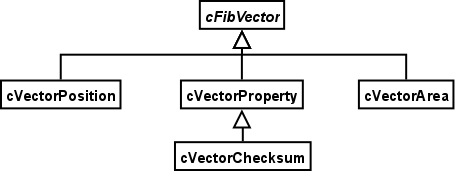
\includegraphics[scale=0.4]{fib_vectors}
\end{center}
\caption{Klassengraph der Fib-Vektoren}
\label{figClassVectors}
\end{figure}


\subsection{Schnittstellenbeschreibung}

\subsubsection{cFibVector}\index{cFibVector}

\textbf{Syntax:} \verb|protected cFibVector(| \\\verb| unsignedIntFib iNumberOfVectorElements=1,| \\\verb| const cFibElement * pDefiningFibElement )|

\bigskip\noindent
Konstruktor eines Vektors, er erzeugt einen Vektors. Da ein allgemeiner Vektor \verb|cFibVector| nicht erzeugt werden kann und soll, ist der Konstruktor au"serhalb der von \verb|cFibVector| abgeleiteten Klassen nicht aufrufbar.

Alle Vektorelemente werden mit 0 initialisiert.

\bigskip\noindent
\textbf{Eingabeparameter:}
\begin{itemize}
 \item \verb|iNumberOfVectorElements|: Die Anzahl der Elemente, welche der Vektor enthalten soll. Standardwert ist 1 .
 \item \verb|pDefiningFibElement|: Ein Zeiger auf das Fib-Element, welches den Vektor enth"alt. Standardwert ist der Nullpointer \verb|NULL|, um anzuzeigen, dass noch kein Fib-Element bekannt ist, welches den Vektor enth"alt.
\end{itemize}

\bigskip\noindent
\textbf{R"uckgabe:} keine


\subsubsection{getElementType}\index{cFibVector!getElementType()}\index{getElementType()}

\textbf{Syntax:} \verb|cTypeElement getElementType() const|

\bigskip\noindent
Diese Methode gibt den Typ des Vektors zur"uck.

\bigskip\noindent
\textbf{Eingabeparameter:} keine

\bigskip\noindent
\textbf{R"uckgabe:} Einen Zeiger auf den Typ des Vektors.


\subsubsection{getNumberOfElements}\index{cFibVector!getNumberOfElements()}\index{getNumberOfElements()}

\textbf{Syntax:} \verb|unsignedIntFib getNumberOfElements() const|

\bigskip\noindent
Diese Methode gibt die Anzahl der Elemente des Vektors zur"uck.

\bigskip\noindent
\textbf{Eingabeparameter:} keine

\bigskip\noindent
\textbf{R"uckgabe:} Die Anzahl der Elemente des Vektors.


\subsubsection{isVariable}\index{cFibVector!isVariable()}\index{isVariable()}

\textbf{Syntax:} \verb|bool isVariable( unsignedIntFib iNumberElement )| \\\verb| const|

\bigskip\noindent
Diese Methode gibt zur"uck, ob das \verb|iNumberElement|'te Element des Vektors eine Variable ist.

\bigskip\noindent
\textbf{Eingabeparameter:}
\begin{itemize}
 \item \verb|iNumberElement|: Die Nummer des Vektorelements, f"ur das zur"uckgegeben werden soll, ob es eine Variable ist.
\end{itemize}

\bigskip\noindent
\textbf{R"uckgabe:} Wenn das \verb|iNumberElement|'te Element des Vektors eine Variable ist, wird \verb|true| (=wahr) zur"uckgegeben, sonst \verb|false| (=falsch).


\subsubsection{getValue}\index{cFibVector!getValue()}\index{getValue()}

\textbf{Syntax:} \verb|doubleFib getValue(| \\\verb| unsignedIntFib iNumberElement ) const|

\bigskip\noindent
Diese Methode gibt den Wert des \verb|iNumberElement|'ten Elements zur"uck.

Dabei wird bei einer Variable ihre Belegung ausgegeben. Ist die Variable nicht belegt, wird der Nullwert des Definitionsbereiches zum Vektorelement zur"uckgegeben.

Der zur"uckgegebene Wert liegt immer im Definitionsbereich des Vektors (auch bez"uglich der anderen Vektorelemente).

\bigskip\noindent
\textbf{Eingabeparameter:}
\begin{itemize}
 \item \verb|iNumberElement|: Die Nummer des Vektorelements, f"ur das der Wert zur"uckgegeben werden soll.
\end{itemize}

\bigskip\noindent
\textbf{R"uckgabe:} Den Wert des \verb|iNumberElement|'ten Elements.


\subsubsection{setValue}\index{cFibVector!setValue()}\index{setValue()}

\textbf{Syntax:} \verb|bool setValue( unsignedIntFib iNumberElement,| \\\verb| doubleFib dValue )|

\bigskip\noindent
Diese Methode setzt das \verb|iNumberElement|'ten Vektorelement auf den Wert \verb|dValue|.

Der Wert \verb|dValue| muss im Definitionsbereich des Vektorelements liegen, um gesetzt werden zu k"onnen. Wenn der Wert \verb|dValue| nicht im Definitionsbereich des Vektorelements liegt, wird das Vektorelement nicht ver"andert und \verb|false| (=falsch) zur"uckgegeben. (Dann sollte eventuell der Definitionsbereich angepasst werden.) Werte die mit der \verb|round|-Methode des zum Vektorelement geh"orenden Definitionsbereich erzeugt wurden (bzw. bei denen die \verb|isElement|-Methode \verb|true| zur"uckgibt), k"onnen immer gesetzt werden.

\bigskip\noindent
\textbf{Eingabeparameter:}
\begin{itemize}
 \item \verb|iNumberElement|: Die Nummer des Vektorelements, f"ur das der Wert \verb|dValue| gesetzt werden soll.
 \item \verb|dValue|: Der Wert \verb|dValue|, welcher gesetzt werden soll.
\end{itemize}

\bigskip\noindent
\textbf{R"uckgabe:} Wenn das \verb|iNumberElement|'te Element des Vektors auf den Wert \verb|dValue| gesetzt wurde, wird \verb|true| (=wahr) zur"uckgegeben, sonst \verb|false| (=falsch).


\subsubsection{getVariable}\index{cFibVector!getVariable()}\index{getVariable()}

\textbf{Syntax:} \verb|cFibVariable *getVariable( unsignedIntFib| \\\verb| iNumberElement )|

\bigskip\noindent
Diese Methode liefert einen Zeiger auf die Variable des \verb|iNumberElement|'ten Vektorelements zur"uck oder \verb|NULL| (Nullpointer), wenn das \verb|iNumber|'te Vektorelement keine Variable ist.

\bigskip\noindent
\textbf{Eingabeparameter:}
\begin{itemize}
 \item \verb|iNumberElement|: Die Nummer des Vektorelements, von dem die Variable zur"uckgegeben werden soll.
\end{itemize}

\bigskip\noindent
\textbf{R"uckgabe:} Einen Zeiger auf die Variable des \verb|iNumberElement|'ten Vektorelements oder \verb|NULL| (Nullpointer), wenn das \verb|iNumberElement|'te Vektorelement keine Variable ist.


\subsubsection{setVariable}\index{cFibVector!setVariable()}\index{setVariable()}

\textbf{Syntax:} \verb|bool setVariable( unsignedIntFib iNumberElement,| \\\verb| cFibVariable *pVariable )|

\bigskip\noindent
Diese Methode setzt das \verb|iNumberElement|'te Vektorelement auf die Variable \verb|pVariable|.

Gibt es kein \verb|iNumberElement|'tes Vektorelement wird \verb|false| (=falsch) zur"uckgegeben.

\bigskip\noindent
\textbf{Eingabeparameter:}
\begin{itemize}
 \item \verb|iNumberElement|: Die Nummer des Vektorelements, f"ur das die Variable \verb|pVariable| gesetzt werden soll.
 \item \verb|pVariable|: Der Zeiger auf die zu setzende Variable.
\end{itemize}

\bigskip\noindent
\textbf{R"uckgabe:} Wenn das \verb|iNumberElement|'te Element des Vektors auf die Variable \verb|pVariable| gesetzt wurde, wird \verb|true| (=wahr) zur"uckgegeben, sonst \verb|false| (=falsch).


\subsubsection{getDomain}\index{cFibVector!getDomain()}\index{getDomain()}

\textbf{Syntax:} \verb|cDomainVectorBasis * getDomain()|

\bigskip\noindent
Diese Methode gibt eine Referenz auf den Definitionsbereich des Vektors zur"uck oder den Nullpointer \verb|NULL|, wenn keine Definitionsbereich f"ur den Vektor definiert ist.
Wenn der Nullpointer \verb|NULL| zur"uckgegeben wurde ist die Standarddomain f"ur den vektor g"ultig.

\bigskip\noindent
\textbf{Eingabeparameter:} keine

\bigskip\noindent
\textbf{R"uckgabe:} Es wird eine Referenz auf den Definitionsbereich des Vektors zur"uckgegeben oder den Nullpointer \verb|NULL|, wenn keine Definitionsbereich f"ur den Vektor definiert ist.


\subsubsection{getDomain}\index{cFibVector!getDomain()}\index{getDomain()}

\textbf{Syntax:} \verb|cDomainSingle *getDomain( unsignedIntFib| \\\verb| iNumberElement )|

\bigskip\noindent
Diese Methode gibt einen Zeiger auf den Definitionsbereich des entsprechenden \verb|iNumberElement|'ten Vektorelements zur"uck oder den Nullpointer \verb|NULL|, wenn keine Definitionsbereich f"ur den Vektor definiert ist.
Wenn der Nullpointer \verb|NULL| zur"uckgegeben wurde ist die Standarddomain f"ur den vektor g"ultig.

\bigskip\noindent
\textbf{Eingabeparameter:}
\begin{itemize}
 \item \verb|iNumberElement|: Die Nummer des Vektorelements, f"ur das der Definitionsbereich zur"uckgegeben werden soll.
\end{itemize}

\bigskip\noindent
\textbf{R"uckgabe:} Es wird einen Zeiger auf den Definitionsbereich des entsprechenden \verb|iNumberElement|'ten Vektorelements oder den Nullpointer \verb|NULL| (wenn keine Definitionsbereich f"ur den Vektor definiert ist) zur"uckgegeben.


\subsubsection{getStandardDomain}\index{cFibVector!getStandardDomain()}\index{getStandardDomai()}

\textbf{Syntax:} \verb|cDomainVectorBasis *getStandardDomain() const|

\bigskip\noindent
Diese Methode gibt eine Referenz auf den Standarddefinitionsbereich des Vektors zur"uck.

\bigskip\noindent
\textbf{Eingabeparameter:} keine

\bigskip\noindent
\textbf{R"uckgabe:} Zur"uckgegeben wird eine Referenz auf den Standarddefinitionsbereich des Vektors.


\subsubsection{getDefiningFibElement}\index{cFibVector!getDefiningFibElement()}\index{getDefiningFibElement()}

\textbf{Syntax:} \verb|cFibElement *getDefiningFibElement() const|

\bigskip\noindent
Diese Methode gibt eine Referenz auf das Fib-Element zur"uck, welches den Vektor definiert bzw. ihn enth"alt.

\bigskip\noindent
\textbf{Eingabeparameter:} keine

\bigskip\noindent
\textbf{R"uckgabe:} Zur"uckgegeben wird eine Referenz auf das Fib-Element, welches den Vektor definiert bzw. enth"alt.


\subsubsection{setDefiningFibElement}\index{cFibVector!setDefiningFibElement()}\index{setDefiningFibElement()}

\textbf{Syntax:} \verb|void setDefiningFibElement(| \\\verb| cFibElement * fibElement=NULL );|

\bigskip\noindent
Diese Methode setzt das Fib-Element, welches den Vektor definiert bzw. enth"alt.

\bigskip\noindent
\textbf{Eingabeparameter:}
\begin{itemize}
 \item \verb|fibElement|: Ein Zeiger auf das Fib-Element, welches den Vektors enth"alt. Standardwert ist der Nullpointer \verb|NULL|, um anzuzeigen das noch kein Fib-Element, welches den Vektors enth"alt, bekannt ist.
\end{itemize}

\bigskip\noindent
\textbf{R"uckgabe:} keine.



\subsection{cVectorPosition}\index{cVectorPosition}\index{cFibVector!cVectorPosition}

\bigskip\noindent
\textbf{Elternklasse:} cFibVector

\bigskip\noindent
\textbf{Standarddefinitionsbereich:} $vector( 2$, $integerB(16)$, $integerB(16) )$

\bigskip\noindent
Dieser Vektor stellt einen Positionsvektor dar. Er kann nur in Punktelementen verwendet werden.


\subsubsection{cVectorPosition}

\textbf{Syntax:} \verb|cVectorPosition(| \\\verb| unsignedIntFib iNumberOfDimensions=2,| \\\verb| cFibElement * pDefiningPointElement=NULL )|

\bigskip\noindent
Der Konstruktor des Positionsvektors, er erstellt einen Positionsvektor.

Initial werden alle Elemente auf den Nullwerte des entsprechenden Definitionsbereichs gesetzt.

\bigskip\noindent
\textbf{Eingabeparameter:}
\begin{itemize}
 \item \verb|iNumberOfDimensions|: Die Anzahl der Dimensionen bzw. Elemente, welche der Positionsvektor enthalten soll. Standardwert ist $2$ .
 \item \verb|pDefiningPointElement|: Ein Zeiger auf das Fib-Element, welches den Vektor enth"alt. Standardwert ist der Nullpointer \verb|NULL|, um anzuzeigen, dass noch kein Fib-Element bekannt ist, welches den Vektor enth"alt.
\end{itemize}

\bigskip\noindent
\textbf{R"uckgabe:} keine


\subsection{cVectorProperty}\index{cFibVector!cVectorProperty}

\bigskip\noindent
\textbf{Elternklasse:} cFibVector

\bigskip\noindent
\textbf{Standarddefinitionsbereich:}  $vector( 0 )$

\bigskip\noindent
Mit diesem Vektor werden die Werte von Eigenschaften gespeichert. Dabei wird der Typ der Eigenschaft, f"ur den der Vektor steht, beim Erzeugen des Objekts festgelegt.


\subsubsection{cVectorProperty}

\textbf{Syntax:} \verb|cVectorProperty( unsignedIntFib uiProperyType,| \\\verb| cFibElement * pDefiningFibElement=NULL )|

\bigskip\noindent
Der Konstruktor des Eigenschaftsvektors, er erstellt einen Eigenschaftsvektor.

Initial werden alle Elemente auf den Nullwerte des entsprechenden Definitionsbereichs gesetzt.

\bigskip\noindent
\textbf{Eingabeparameter:}
\begin{itemize}
 \item \verb|uiProperyType|: Der Typ der Eigenschaft. Dieses ist ein Wert, so wie er in Tabelle \ref{tablePropertyNamen} auf Seite \pageref{tablePropertyNamen} angegeben wird.
 \item \verb|pDefiningFibElement|: Ein Zeiger auf das Fib-Element, welches den Vektor enth"alt. Standardwert ist der Nullpointer \verb|NULL|, um anzuzeigen, dass noch kein Fib-Element bekannt ist, welches den Vektor enth"alt.
\end{itemize}

\bigskip\noindent
\textbf{R"uckgabe:} keine


\subsubsection{cVectorProperty}

\textbf{Syntax:} \verb|cVectorProperty( unsignedIntFib uiProperyType,| \\\verb| unsignedIntFib iNumberOfVectorElements=1,| \\\verb| cFibElement * pDefiningFibElement=NULL )|

\bigskip\noindent
Der Konstruktor des Eigenschaftsvektors, er erstellt einen Eigenschaftsvektor.

Dieser Konstruktor sollte verwendet werden, wenn f"ur die Eigenschaft vom Typ \verb|iProperyType| kein korrekter Standarddefinitionsbereich existiert. (z. B. wie bei den ``Product Properties`` siehe Tabelle \ref{tablePropertyNamen} auf Seite \pageref{tablePropertyNamen})

Initial werden alle Elemente auf den Nullwerte des entsprechenden Definitionsbereichs gesetzt.

\bigskip\noindent
\textbf{Eingabeparameter:}
\begin{itemize}
 \item \verb|uiProperyType|: Der Typ der Eigenschaft. Dieses ist ein Wert, so wie er in Tabelle \ref{tablePropertyNamen} auf Seite \pageref{tablePropertyNamen} angegeben wird.
 \item \verb|iNumberOfVectorElements|: Die Anzahl der Elemente, welche der Vektor enthalten soll. Standardwert ist $1$ .
 \item \verb|pDefiningFibElement|: Ein Zeiger auf das Fib-Element, welches den Vektor enth"alt. Standardwert ist der Nullpointer \verb|NULL|, um anzuzeigen, das noch kein Fib-Element bekannt ist, welches den Vektor enth"alt.
\end{itemize}

\bigskip\noindent
\textbf{R"uckgabe:} keine


\subsubsection{getPropertyType}\index{cVectorProperty!getPropertyType()}\index{getPropertyType()}

\textbf{Syntax:} \verb|unsignedIntFib getPropertyType()|

\bigskip\noindent
Diese Methode gibt den Typ der Eigenschaft zur"uck, so wie er in Tabelle \ref{tablePropertyNamen} auf Seite \pageref{tablePropertyNamen} angegeben wird.

\bigskip\noindent
\textbf{Eingabeparameter:} keine

\bigskip\noindent
\textbf{R"uckgabe:} Den Typ der Eigenschaft.


\subsubsection{cVectorChecksum}\index{cFibVector!cVectorChecksum}

\bigskip\noindent
\textbf{Elternklasse:} cVectorProperty

\bigskip\noindent
\textbf{Standarddefinitionsbereich:}

$vector( 3$, $integerB(4)$,  $integerB(8)$, $integerB(8) )$

\bigskip\noindent
\textbf{Kompatible zu:} Alle Vektoren mit drei Elementen, deren Definitionsbereich aus den nat"urlichen Zahlen kommen.

\bigskip\noindent
Dieser Vektor dient der Typsicherheit des Checksummenvektors im root-Element. Er hat keine eigenen Methoden.


\paragraph{cVectorChecksum}

\ \\\\\noindent
\textbf{Syntax:} \verb|cVectorChecksum(| \\\verb|cFibElement * pDefiningFibElement=NULL )|

\bigskip\noindent
Der Konstruktor des Eigenschaftsvektors f"ur die Checksummeneigenschaft, er erstellt einen Eigenschaftsvektor f"ur die Checksummeneigenschaft.

Initial werden alle Elemente auf den Nullwerte des entsprechenden Definitionsbereichs gesetzt.

%TODO besser gute komprimierungswerte?

\bigskip\noindent
\textbf{Eingabeparameter:}
\begin{itemize}
 \item \verb|pDefiningFibElement|: Ein Zeiger auf das Fib-Element, welches den Vektor enth"alt. Standardwert ist der Nullpointer \verb|NULL|, um anzuzeigen, dass noch kein Fib-Element bekannt ist, welches den Vektor enth"alt.
\end{itemize}


\bigskip\noindent
\textbf{R"uckgabe:} keine


\subsection{cVectorArea}\index{cFibVector!cVectorArea}

\bigskip\noindent
\textbf{Elternklasse:} cFibVector

\bigskip\noindent
\textbf{Standarddefinitionsbereich:} $vector( 2$, $integerB(32)$,  $integerB(32) )$ (Standarddefinitionsbereich von \verb|cTypeArea|)

\bigskip\noindent
Dieser Vektor h"alt die Werte f"ur die untere und obere Grenze eines Unterbereichs (inklusive Grenzen). Beide Werte f"ur die Grenzen sind Ganzzahlen.


\subsubsection{cVectorArea}

\textbf{Syntax 1:} \verb|cVectorArea( longFib lLowerBound,| \\\verb| longFib lUpperBound, | \\\verb|cFibElement * pDefiningFibElement=NULL )|

\noindent
\textbf{Syntax 2:} \verb|cVectorArea( longFib lLowerBound,| \\\verb| cFibVariable & vUpperBound, | \\\verb|cFibElement * pDefiningFibElement=NULL ) )|

\noindent
\textbf{Syntax 3:} \verb|cVectorArea( cFibVariable & vLowerBound,| \\\verb| longFib lUpperBound, | \\\verb|cFibElement * pDefiningFibElement=NULL ) )|

\noindent
\textbf{Syntax 4:} \verb|cVectorArea( cFibVariable & vLowerBound,| \\\verb| cFibVariable & vUpperBound, | \\\verb|cFibElement * pDefiningFibElement=NULL ) )|

\bigskip\noindent
Der Konstruktoren des Bereichsvektors, sie erstellen jeweils einen Bereichsvektor.

\bigskip\noindent
\textbf{Eingabeparameter:}
\begin{itemize}
 \item \verb|lLowerBound|: Die unter Grenze des Bereichs, den der Vektor repr"asentiert.
 \item \verb|vLowerBound|: Eine Referenz auf die Variable, welche die unter Grenze des Bereichs bestimmt, den der Vektor repr"asentiert.
 \item \verb|lUpperBound|: Die ober Grenze des Bereichs, den der Vektor repr"asentiert.
 \item \verb|vUpperBound|: Eine Referenz auf die Variable, welche die obere Grenze des Bereichs bestimmt, den der Vektor repr"asentiert.
 \item \verb|pDefiningFibElement|: Ein Zeiger auf das Fib-Element, welches den Vektor enth"alt. Standardwert ist der Nullpointer \verb|NULL|, um anzuzeigen, dass noch kein Fib-Element bekannt ist, welches den Vektor enth"alt.
\end{itemize}

\bigskip\noindent
\textbf{R"uckgabe:} keine


\subsubsection{getLowerBound}\index{cVectorArea!getLowerBound()}\index{getLowerBound()}

\textbf{Syntax:} \verb|longFib getLowerBound() const|

\bigskip\noindent
Diese Methode gibt die untere Grenze des Bereichs zur"uck.

Dabei wird bei einer Variable ihre Belegung ausgegeben. Ist die Variable nicht belegt, wird der Nullwert des Definitionsbereiches zum Bereichstyp (bzw. des Vektorelements) zur"uckgegeben.

\bigskip\noindent
\textbf{Eingabeparameter:} keine

\bigskip\noindent
\textbf{R"uckgabe:} Die untere Grenze des Bereichs.


\subsubsection{getUpperBound}\index{cVectorArea!getUpperBound()}\index{getUpperBound()}

\textbf{Syntax:} \verb|longFib getUpperBound() const|

\bigskip\noindent
Diese Methode gibt die obere Grenze des Bereichs zur"uck.

Dabei wird bei einer Variable ihre Belegung ausgegeben. Ist die Variable nicht belegt, wird der Nullwert des Definitionsbereiches zum Bereichstyp (bzw. des Vektorelements) zur"uckgegeben.

\bigskip\noindent
\textbf{Eingabeparameter:} keine

\bigskip\noindent
\textbf{R"uckgabe:} Die ober Grenze des Bereichs.


\subsubsection{getAreaValues}\index{cVectorArea!getAreaValues()}\index{getAreaValues()}

\textbf{Syntax:} \verb|list<longFib> getAreaValues() const|

\bigskip\noindent
Diese Methode gibt alle Werte die im Bereich liegen zur"uck.

Dies sind alle Ganzzahlen zwischen der oberen und unteren Grenze des Bereichs (inclusive der Grenzen, wenn diese jeweils Ganzzahlen ist).

Dabei wird bei einer Variable als Grenze ihre Belegung ber"ucksichtigt. Ist die Variable nicht belegt, wird der Nullwert des Definitionsbereiches zum Bereichstyps (bzw. des Vektorelements) ber"ucksichtigt.

\bigskip\noindent
\textbf{Eingabeparameter:} keine

\bigskip\noindent
\textbf{R"uckgabe:} Zur"uckgegeben werden alle Werte, die im Bereich liegen.


\subsubsection{setLowerBoundValue}\index{cVectorArea!setLowerBoundValue()}\index{setLowerBoundValue()}

\textbf{Syntax:} \verb|bool setLowerBoundValue( longFib lValue )|

\bigskip\noindent
Diese Methode setzt die untere Grenze des Bereichs auf den Wert \verb|lValue|.

Der Wert \verb|lValue| muss im Definitionsbereich des Vektorelements bzw. des Bereichstyps liegen, um gesetzt werden zu k"onnen. Wenn der Wert \verb|lValue| nicht im Definitionsbereich des Vektorelements liegt, wird das Vektorelement nicht ver"andert und \verb|false| (=falsch) zur"uckgegeben. (Dann sollte eventuell der Definitionsbereich entsprechend angepasst werden.) Werte die mit der \verb|round|-Methode des zum Vektorelement geh"orenden Definitionsbereich erzeugt wurden (bzw. bei denen die \verb|isElement|-Methode \verb|true| zur"uckgibt), k"onnen immer gesetzt werden.

\bigskip\noindent
\textbf{Eingabeparameter:}
\begin{itemize}
 \item \verb|lValue|: Der f"ur die untere Grenze des Bereichs zu setzende Wert.
\end{itemize}

\bigskip\noindent
\textbf{R"uckgabe:} Wenn die untere Grenze des Bereichs auf den Wert \verb|lValue| gesetzt wurde, wird \verb|true| (=wahr) zur"uckgegeben, sonst \verb|false| (=falsch).


\subsubsection{setUpperBoundValue}\index{cVectorArea!setUpperBoundValue()}\index{setUpperBoundValue()}

\textbf{Syntax:} \verb|bool setUpperBoundValue( longFib lValue )|

\bigskip\noindent
Diese Methode setzt die obere Grenze des Bereichs auf den Wert \verb|lValue|.

Der Wert \verb|lValue| muss im Definitionsbereich des Vektorelements bzw. des Bereichstyps liegen, um gesetzt werden zu k"onnen. Wenn der Wert \verb|lValue| nicht im Definitionsbereich des Vektorelements liegt, wird das Vektorelement nicht ver"andert und \verb|false| (=falsch) zur"uckgegeben. (Dann sollte eventuell der Definitionsbereich entsprechend angepasst werden.) Werte die mit der \verb|round|-Methode des zum Vektorelement geh"orenden Definitionsbereich erzeugt wurden (bzw. bei denen die \verb|isElement|-Methode \verb|true| zur"uckgibt), k"onnen immer gesetzt werden.

\bigskip\noindent
\textbf{Eingabeparameter:}
\begin{itemize}
 \item \verb|lValue|: Der f"ur die obere Grenze des Bereichs zu setzende Wert.
\end{itemize}

\bigskip\noindent
\textbf{R"uckgabe:} Wenn die obere Grenze des Bereichs auf den Wert \verb|lValue| gesetzt wurde, wird \verb|true| (=wahr) zur"uckgegeben, sonst \verb|false| (=falsch).


\subsubsection{setLowerBoundVariable}\index{cVectorArea!setLowerBoundVariable()}\index{setLowerBoundVariable()}

\textbf{Syntax:} \verb|bool setLowerBoundVariable( cFibVariable| \\\verb| *pVariable )|

\bigskip\noindent
Diese Methode setzt die untere Grenze des Bereichs auf die Variable \verb|pVariable|.

\bigskip\noindent
\textbf{Eingabeparameter:}
\begin{itemize}
 \item \verb|pVariable|: Der Zeiger auf die zu setzende Variable.
\end{itemize}

\bigskip\noindent
\textbf{R"uckgabe:} Wenn unter Grenze des Bereichs auf die Variable \verb|pVariable| gesetzt wurde, wird \verb|true| (=wahr) zur"uckgegeben, sonst \verb|false| (=falsch).


\subsubsection{setUpperBoundVariable}\index{cVectorArea!setUpperBoundVariable()}\index{setUpperBoundVariable()}

\textbf{Syntax:} \verb|bool setUpperBoundVariable( cFibVariable| \\\verb| *pVariable )|

\bigskip\noindent
Diese Methode setzt die obere Grenze des Bereichs auf die Variable \verb|pVariable|.

\bigskip\noindent
\textbf{Eingabeparameter:}
\begin{itemize}
 \item \verb|pVariable|: Der Zeiger auf f"ur die zu setzende Variable.
\end{itemize}

\bigskip\noindent
\textbf{R"uckgabe:} Wenn obere Grenze des Bereichs auf die Variable \verb|pVariable| gesetzt wurde, wird \verb|true| (=wahr) zur"uckgegeben, sonst \verb|false| (=falsch).


\subsection{cVectorExtObject}\index{cVectorExtObject}\index{cFibVector!cVectorExtObject}

\bigskip\noindent
\textbf{Elternklasse:} cFibVector

\bigskip\noindent
\textbf{Standarddefinitionsbereich:} $vectorOpenEnd( integerB(8) )$ (Standarddefinitionsbereich von \verb|cTypeExtObjectInput|)

\bigskip\noindent
Dieser Vektor stellt einen Satz bzw. Vektor von Zahlen dar. Er kann nur im externen Objekt Element verwendet werden (siehe Abschnitt \ref{secCExtObjectElement} auf Seite \pageref{secCExtObjectElement} und Abschnitt \ref{secExtObjectElement} auf Seite \pageref{secExtObjectElement} ) .


\subsubsection{cVectorExtObject}

\textbf{Syntax:} \verb|cVectorExtObject(| \\\verb| unsignedIntFib iNumberOfElements=0,| \\\verb| cFibElement * pDefiningMatrixElement=NULL )|

\bigskip\noindent
Der Konstruktor des Vektors f"ur das externen Objekt Element.

Initial werden alle Elemente auf den Nullwerte des entsprechenden Definitionsbereichs gesetzt.

\bigskip\noindent
\textbf{Eingabeparameter:}
\begin{itemize}
 \item \verb|iNumberOfDimensions|: Die Anzahl der Elemente, welche der Vektor enthalten soll. Standardwert ist $0$ .
 \item \verb|pDefiningPointElement|: Ein Zeiger auf das Fib-Element, welches den Vektor enth"alt. Standardwert ist der Nullpointer \verb|NULL|, um anzuzeigen, dass noch kein Fib-Element bekannt ist, welches den Vektor enth"alt.
\end{itemize}

\bigskip\noindent
\textbf{R"uckgabe:} keine


\subsection{cVectorExtSubobject}\index{cVectorExtSubobject}\index{cFibVector!cVectorExtSubobject}

\bigskip\noindent
\textbf{Elternklasse:} cFibVector

\bigskip\noindent
\textbf{Standarddefinitionsbereich:} $vector( 0 )$ (Standarddefinitionsbereich von \verb|cTypeExtSubobject|)

\bigskip\noindent
Dieser Vektor stellt einen Satz bzw. Vektor von Zahlen dar. Er kann nur im externen Unterobjekt Element verwendet werden (siehe Abschnitt \ref{secCExtSubobjectElement} auf Seite \pageref{secCExtSubobjectElement} und Abschnitt \ref{secExtSubobjectElement} auf Seite \pageref{secExtSubobjectElement} ) .


\subsubsection{cVectorExtSubobject}

\textbf{Syntax:} \verb|cVectorExtSubobject(| \\\verb| unsignedIntFib iNumberOfElements=0,| \\\verb| cFibElement * pDefiningMatrixElement=NULL )|

\bigskip\noindent
Der Konstruktor des Vektors f"ur das externen Unterobjekt Element.

Initial werden alle Elemente auf den Nullwerte des entsprechenden Definitionsbereichs gesetzt.

\bigskip\noindent
\textbf{Eingabeparameter:}
\begin{itemize}
 \item \verb|iNumberOfDimensions|: Die Anzahl der Elemente, welche der Vektor enthalten soll. Standardwert ist $0$ .
 \item \verb|pDefiningPointElement|: Ein Zeiger auf das Fib-Element, welches den Vektor enth"alt. Standardwert ist der Nullpointer \verb|NULL|, um anzuzeigen, dass noch kein Fib-Element bekannt ist, welches den Vektor enth"alt.
\end{itemize}

\bigskip\noindent
\textbf{R"uckgabe:} keine


\subsection{cVectorFibSet}\index{cVectorFibSet}\index{cFibVector!cVectorFibSet}

\bigskip\noindent
\textbf{Elternklasse:} cFibVector

\bigskip\noindent
\textbf{Standarddefinitionsbereich:} $vectorOpenEnd( 1,$ $integerB(32) )$ (dritter Unterdefinitionsbereich vom Standarddefinitionsbereich von \verb|cTypeFibSet|)

\bigskip\noindent
Dieser Vektor stellt einen Satz bzw. Vektor von Zahlen dar. Er kann nur im set-Element verwendet werden (siehe Abschnitt \ref{secCFibSetElement} auf Seite \pageref{secCFibSetElement} und Abschnitt \ref{secFibSetElement} auf Seite \pageref{secFibSetElement} ) .


\subsubsection{cVectorFibSet}

\textbf{Syntax:} \verb|cVectorFibSet(| \\\verb| unsignedIntFib iNumberOfElements=2,| \\\verb| cFibElement * pDefiningSetElement=NULL )|

\bigskip\noindent
Der Konstruktor des Vektors f"ur das set-Element.

Initial werden alle Elemente auf den Nullwerte des entsprechenden Definitionsbereichs gesetzt.

\bigskip\noindent
\textbf{Eingabeparameter:}
\begin{itemize}
 \item \verb|iNumberOfElements|: Die Anzahl der Elemente, welche der Vektor enthalten soll. Standardwert ist $2$ .
 \item \verb|pDefiningPointElement|: Ein Zeiger auf das Fib-Element, welches den Vektor enth"alt. Standardwert ist der Nullpointer \verb|NULL|, um anzuzeigen, dass noch kein Fib-Element bekannt ist, welches den Vektor enth"alt.
\end{itemize}

\bigskip\noindent
\textbf{R"uckgabe:} keine


\subsection{cVectorFibMatrix}\index{cVectorFibMatrix}\index{cFibVector!cVectorFibMatrix}

\bigskip\noindent
\textbf{Elternklasse:} cFibVector

\bigskip\noindent
\textbf{Standarddefinitionsbereich:} $vectorOpenEnd( 1,$ $integerB(32) )$ (vierter Unterdefinitionsbereich vom Standarddefinitionsbereich von \verb|cTypeFibMatrix|)

\bigskip\noindent
Dieser Vektor stellt einen Satz bzw. Vektor von Zahlen dar. Er kann nur im Matrixelement verwendet werden (siehe Abschnitt \ref{secCFibMatrixElement} auf Seite \pageref{secCFibMatrixElement} und Abschnitt \ref{secFibMatrixElement} auf Seite \pageref{secFibMatrixElement} ) .


\subsubsection{cVectorFibMatrix}

\textbf{Syntax:} \verb|cVectorFibMatrix(| \\\verb| unsignedIntFib iNumberOfElements=2,| \\\verb| cFibElement * pDefiningMatrixElement=NULL )|

\bigskip\noindent
Der Konstruktor des Vektors f"ur das Matrixelement.

Initial werden alle Elemente auf den Nullwerte des entsprechenden Definitionsbereichs gesetzt.

\bigskip\noindent
\textbf{Eingabeparameter:}
\begin{itemize}
 \item \verb|iNumberOfElements|: Die Anzahl der Elemente, welche der Vektor enthalten soll. Standardwert ist $2$ .
 \item \verb|pDefiningPointElement|: Ein Zeiger auf das Fib-Element, welches den Vektor enth"alt. Standardwert ist der Nullpointer \verb|NULL|, um anzuzeigen, dass noch kein Fib-Element bekannt ist, welches den Vektor enth"alt.
\end{itemize}

\bigskip\noindent
\textbf{R"uckgabe:} keine



\section{cFibVariable}\index{cFibVariable}

Die Klasse \verb|cFibVariable| stellt Variablen f"ur Fib-Objekte dar. Jede Variable muss von einem Fib-Element definiert werden. Nur Fib-Elemente k"onnen deshalb Instanzen von \verb|cFibVariable| erzeugen.

Wenn Variablen in einem Fib-Element verwendet werden, sollte die Variable immer "uber dem Fib-Element definiert werden.

Jede Fib-Variable h"alt sich eine Liste mit Fib-Elementen in den die Variable verwendet wird, sowie eine Referenz auf das Fib-Element in dem die Fib-Variable definiert wird.


\subsection{Schnittstellenbeschreibung}


\subsubsection{cFibVariable}\index{cFibVariable}

\textbf{Syntax:} \verb|cFibVariable(| \\\verb| const cFibElement * pDefiningFibElement )|

\bigskip\noindent
Konstruktor einer Variable, er erzeugt eine Variable.

\bigskip\noindent
\textbf{Eingabeparameter:}
\begin{itemize}
 \item \verb|pDefiningFibElement|: Ein Zeiger auf das Fib-Element, das diese Variable definiert.
\end{itemize}

\bigskip\noindent
\textbf{R"uckgabe:} keine


\subsubsection{getValue}\index{cFibVariable!getValue()}\index{getValue()}

\textbf{Syntax:} \verb|doubleFib getValue() const|

\bigskip\noindent
Diese Methode gibt den Wert der Variable zur"uck oder $0$ wenn, der Variablenwert undefiniert ist.

\bigskip\noindent
\textbf{Eingabeparameter:} keine

\bigskip\noindent
\textbf{R"uckgabe:} Der Wert der Variable oder $0$, wenn der Variablenwert undefiniert ist.


\subsubsection{getIntegerValue}\index{cFibVariable!getIntegerValue()}\index{getIntegerValue}

\textbf{Syntax:} \verb|longFib getIntegerValue() const|

\bigskip\noindent
Diese Methode gibt den Wert der Variable als Ganzzahl zur"uck oder $0$ wenn, der Variablenwert undefiniert ist.

Ist der Inhalt der Variable eine Gleitkommazahl oder skalierte Ganzzahl, wird er auf eine Ganzzahl gerundet und ausgegeben.

Dies ist beispielsweise n"utzlich, wenn der Vektor, in dem die Variable verwendet wird, nur Ganzzahlen enthalten darf (wie z. B. bei Unterbereichsvektoren \verb|cVectorArea|).

\bigskip\noindent
\textbf{Eingabeparameter:} keine

\bigskip\noindent
\textbf{R"uckgabe:} Der Wert der Variable als Ganzzahl oder $0$, wenn der Variablenwert undefiniert ist.


\subsubsection{setValue}\index{cFibVariable!setValue()}\index{setValue()}

\textbf{Syntax:} \verb|void setValue( doubleFib dValue )|

\bigskip\noindent
Diese Methode setzt den Wert der Variable auf den "ubergebenen Wert \verb|dValue|.

Diese Methode ist beispielsweise bei Eingabevariablen des obersten root-\-Ele\-men\-ts n"utzlich.

\bigskip\noindent
\textbf{Eingabeparameter:}
\begin{itemize}
 \item \verb|dValue|: Der Wert, auf den die Variable zu setzen ist.
\end{itemize}

\bigskip\noindent
\textbf{R"uckgabe:} keine


\subsubsection{setIntegerValue}\index{cFibVariable!setIntegerValue()}\index{setIntegerValue()}

\textbf{Syntax:} \verb|void setIntegerValue( longFib lValue )|

\bigskip\noindent
Diese Methode setzt den Wert der Variable auf den "ubergebenen Ganzzahlwert \verb|lValue|.

Diese Methode ist beispielsweise bei Eingabevariablen des obersten root-\-Ele\-men\-ts n"utzlich.

Durch Eingabe eines Ganzzahlwertes k"onnte unter anderem die Sprache oder der Untertitel ausgew"ahlt werden. Gleitkommazahlen k"onnten in solchen Situationen zu Rundungsfehlern f"uhren.

\bigskip\noindent
\textbf{Eingabeparameter:}
\begin{itemize}
 \item \verb|lValue|: Der Ganzzahlwert, auf den die Variable zu setzen ist.
\end{itemize}

\bigskip\noindent
\textbf{R"uckgabe:} keine


\subsubsection{getDefiningElement}\index{cFibVariable!getDefiningElement()}\index{getDefiningElement()}

\textbf{Syntax:} \verb|cFibElement * getDefiningElement() const|

\bigskip\noindent
Diese Methode gibt ein Zeiger auf das Fib-Element zur"uck, in dem die Variable definiert wird.

\bigskip\noindent
\textbf{Eingabeparameter:} keine

\bigskip\noindent
\textbf{R"uckgabe:} Ein Zeiger auf das Fib-Element, in dem die Variable definiert wird.


\subsubsection{getNumberOfUsingElements}\index{cFibVariable!getNumberOfUsingElements()}\index{getNumberOfUsingElements()}

\textbf{Syntax:} \verb|unsignedIntFib getNumberOfUsingElements()|

\bigskip\noindent
Diese Methode gibt die Anzahl der Fib-Elemente zur"uck, in denen die Variable benutzt wird.

Wenn dieser Wert beispielsweise 0 ist, kann das Fib-Element, das die Variable definiert, gel"oscht werden.

\bigskip\noindent
\textbf{Eingabeparameter:} keine

\bigskip\noindent
\textbf{R"uckgabe:} Zur"uckgegeben wird die Anzahl der Fib-Element in denen die Variable benutzt wird.


\subsubsection{registerUsingElement}\index{cFibVariable!registerUsingElement()}\index{registerUsingElement()}

\textbf{Syntax:} \verb|protected void registerUsingElement(| \\\verb| cFibElement * usingElement )|

\bigskip\noindent
Diese Methode registriert das Fib-Element \verb|usingElement| als ein Fib-Element, dass die Variable benutzt.

\bigskip\noindent
\textbf{Eingabeparameter:}
\begin{itemize}
 \item \verb|usingElement|: Ein Zeiger auf das Fib-Element, das diese Variable benutzt.
\end{itemize}

\bigskip\noindent
\textbf{R"uckgabe:} keine


\subsubsection{unregisterUsingElement}\index{cFibVariable!unregisterUsingElement()}\index{unregisterUsingElement()}

\textbf{Syntax:} \verb|protected void unregisterUsingElement(| \\\verb| cFibElement * usingElement )|

\bigskip\noindent
Diese Methode deregistriert das Fib-Element \verb|usingElement| als ein Fib-Element, dass die Variable benutzt. Damit wird der Variable angezeigt, dass das Fib-Element \verb|usingElement| die Variable nicht mehr ben"otigt.

\bigskip\noindent
\textbf{Eingabeparameter:}
\begin{itemize}
 \item \verb|usingElement|: Ein Zeiger auf das Fib-Element, das diese Variable nicht mehr benutzt.
\end{itemize}

\bigskip\noindent
\textbf{R"uckgabe:} keine


\subsubsection{getUsingElements}\index{cFibVariable!getUsingElements()}\index{getUsingElements()}

\textbf{Syntax:} \verb|set< cFibElement* > getUsingElements()|

\bigskip\noindent
Diese Methode gibt eine Menge mit den Zeigern auf die Fib-Elemente zur"uck, in denen die Variable benutzt wird.

Dadurch kann die Variable beispielsweise leichter ersetzt werden, als wenn der gesamte Fib-Unterbaum, "uber den die Variable definierenden Fib-Element, nach der Variable durchsucht werden m"usste.

\bigskip\noindent
\textbf{Eingabeparameter:} keine

\bigskip\noindent
\textbf{R"uckgabe:} Zur"uckgegeben wird eine Menge mit den Zeigern auf die Fib-Elemente, in denen die Variable benutzt wird.



\section{Fib-Unterfunktionen cUnderFunction}\index{Funktion!cUnderFunction}\index{cUnderFunction}\index{Funktion}

Die Klasse \verb|cUnderFunction| ist die Basisklasse aller Unterfunktionen. Aus Unterfunktionen werden Funktionen (mit der Struktur von B"aumen) zusammengestellt. (siehe Abschnitt \ref{fibFunction} auf Seite\pageref{fibFunction} )

Die Klasse \verb|cUnderFunction| dient als Basisklasse aller Unterfunktionen. Von der Klasse \verb|cUnderFunction| k"onnen keine Instanzen erzeugt werden.

Bei der Auswertung von Unterfunktionen ist f"ur den erzeugten Wert der Definitionsbereich f"ur Unterfunktionenen nicht relevant. Wenn also beispielsweise der Definitionsbereich f"ur Unterfunktionenen nur Ganzzahlen enth"alt und eine Unterfunktionen zu $1,5$ ausgewertet wird, wird dieser Wert $1,5$ sowohl von anderen Unterfunktionen direkt (ohne Rundung) verwendet werden, als auch die definierte Variable eines Funktionselements den Wert $1,5$ annehemen.
Der Definitionsbereich f"ur Unterfunktionenen kommt nur zur Anwendung, wenn die Unterfunktion einen Wert enth"alt (also wenn die Unterfunktion \verb|cFunctionValue| ist), oder wenn eine Unterfunktion fehlt und desshalb anstatt ihr der Nullwert des Definitionsbereichs eingesetzt werden soll.

In Abbildung \ref{figClassUnderfunctions} ist ein Klassendiagramm der Unterfunktionen zu sehen.

\begin{figure}[htbp]
\begin{center}
  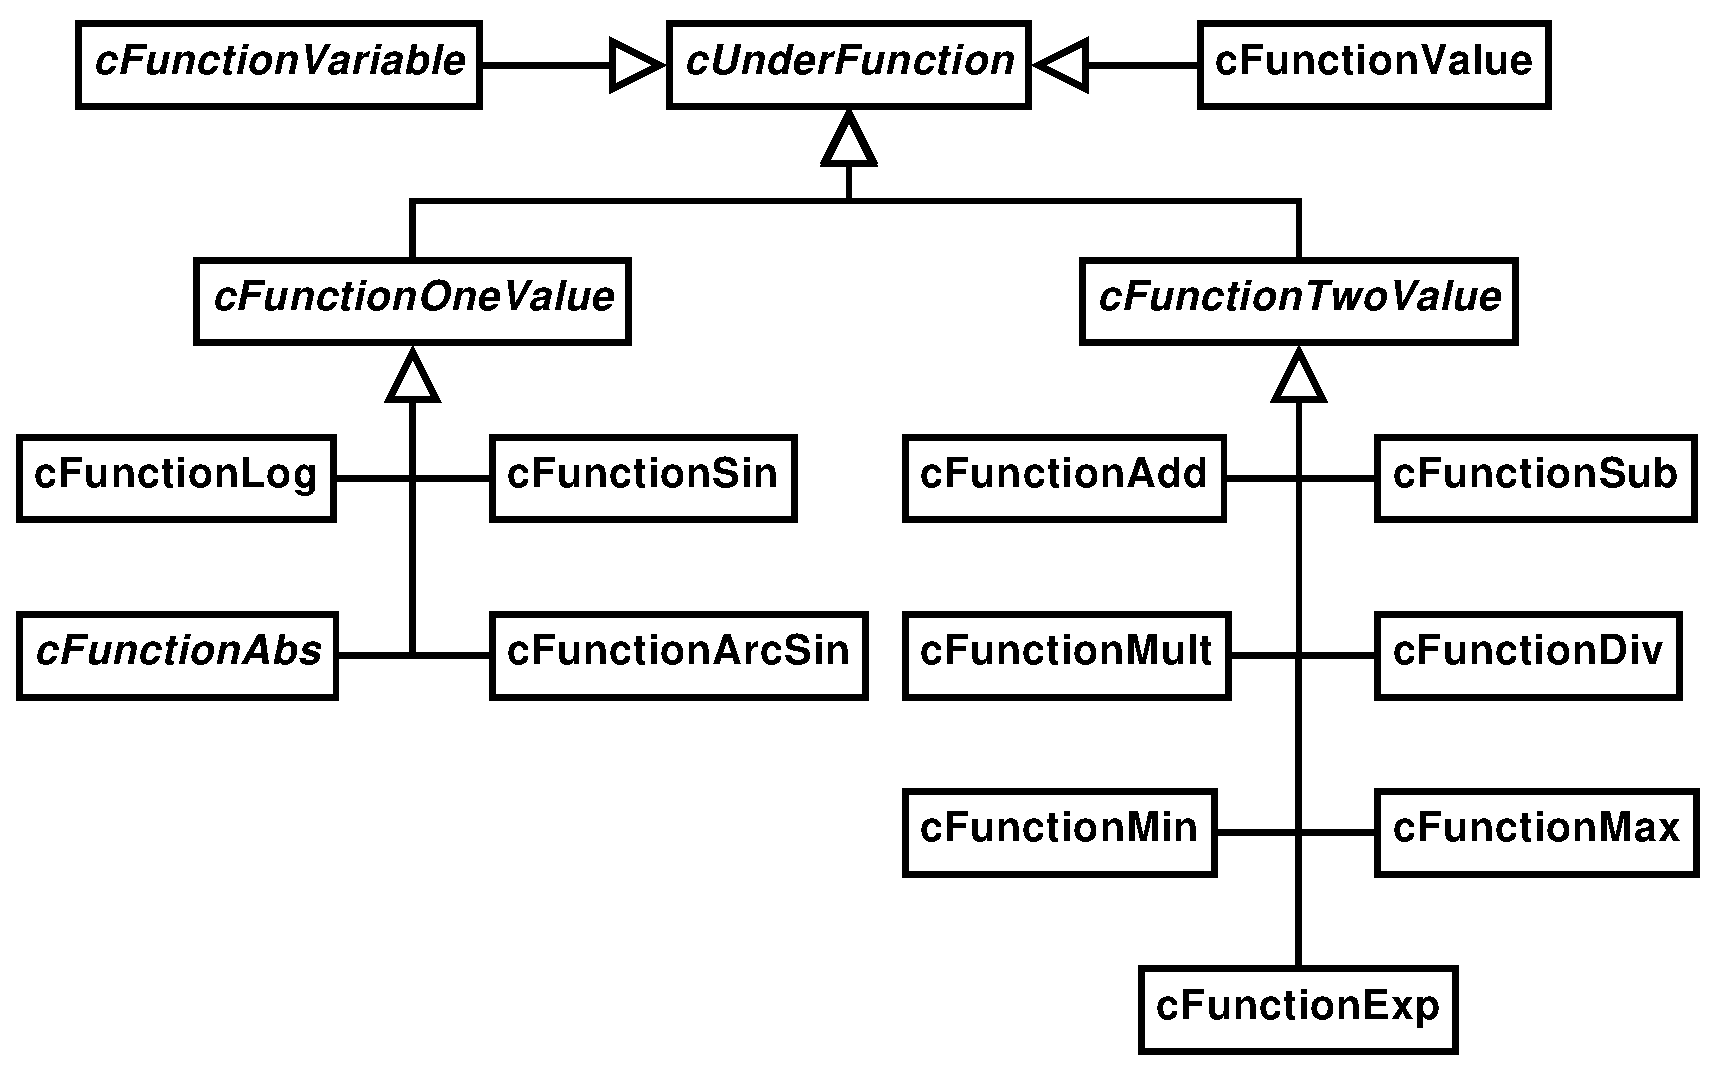
\includegraphics[scale=0.4]{fib_underfunctions}
\end{center}
\caption{Klassengraph der Unterfunktionen}
\label{figClassUnderfunctions}
\end{figure}


\bigskip\noindent
Es gibt drei Arten von Unterfunktionen:
\begin{itemize}
 \item Nullstellige (keine enthaltenden Unterfunktionen)
 \item Einstellige (einen Eingabeparameter bzw. enthaltende Unterfunktionen)
 \item Zweistellige (zwei Eingabeparameter bzw. enthaltende Unterfunktionen)
\end{itemize}

\bigskip\noindent
Die Klassen f"ur die nullstelligen Funktionen sind:
\begin{itemize}
 \item \verb|cFunctionValue|: F"ur einen Wert bzw. eine Konstante.
 \item \verb|cFunctionVariable|: F"ur eine Variable, die "uber dem Fib-Element, welches die Unterfunktion enth"alt, definiert wird.
\end{itemize}

\bigskip\noindent
Die Klassen, welche die einstelligen Funktionen implementieren, werden von der Basisklasse \verb|cFunctionOneValue| abgeleitet.

\bigskip\noindent
Zu diesen einstelligen Funktionen geh"oren:
\begin{itemize}
 \item \verb|cFunctionLog|: Logarithmus
 \item \verb|cFunctionSin|: Sinusfunktion
 \item \verb|cFunctionArcsin|: Arkussinusfunktion
 \item \verb|cFunctionAbs|: Absolutwert
 \item \verb|cFunctionRound|: Runden
\end{itemize}


\bigskip\noindent
Die Klassen, welche die zweistelligen Funktionen implementieren, werden von der Basisklasse \verb|cFunctionTwoValue| abgeleitet.

\bigskip\noindent
Zu diesen zweistelligen Funktionen geh"oren:
\begin{itemize}
 \item \verb|cFunctionAdd|: Addition
 \item \verb|cFunctionSub|: Subtraktion
 \item \verb|cFunctionMult|: Multiplikation
 \item \verb|cFunctionDiv|: Division
 \item \verb|cFunctionExp|: Exponent
 \item \verb|cFunctionMin|: Minimum
 \item \verb|cFunctionMax|: Maximum
 \item \verb|cFunctionIf|: If-Funktion
 \item \verb|cFunctionDelay|: Delay-Funktion
\end{itemize}


\subsection{Schnittstellenbeschreibung}

\subsubsection{getValue}\index{cUnderFunction!getValue()}\index{getValue()}

\textbf{Syntax:} \verb|doubleFib getValue() const|

\bigskip\noindent
Diese Methode berechnet den Wert der Unterfunktion. Dabei werden in der Unterfunktion enthaltenden Unterfunktionen ausgewertet bzw. deren Wert berechnet.

Wenn eine Unterfunktion der Unterfunktion nicht existiert (dies w"are eine ung"ultige Unterfunktion), wird f"ur sie der Nullwert des Definitionsbereichs f"ur Unterfunktionen angenommen.

\bigskip\noindent
\textbf{Eingabeparameter:} keine

\bigskip\noindent
\textbf{R"uckgabe:} Den berechneten Wert der Unterfunktion.


\subsubsection{getType}\index{cUnderFunction!getType()}\index{getType()}

\textbf{Syntax:} \verb|intFib getType() const|

\bigskip\noindent
Diese Methode gibt eine Ganzzahl zur"uck, "uber die der Typ der Unterfunktion bestimmt werden kann. F"ur diese Typen werden auch Konstanten in der Klasse \verb|cUnderFunction| definiert.

\bigskip\noindent
\textbf{M"ogliche Typen sind:}

\noindent
\begin{tabular}{|p{10mm}|p{60mm}|p{40mm}|}\hline
	Typ\-zahl & Unterfunktion & Konstante \\\hline\hline
	00 & \verb|cFunctionValue|: F"ur einen Wert bzw. eine Konstante. & \verb|FUNCTION_VALUE| \\\hline
	01 & \verb|cFunctionVariable|: F"ur eine Variable, die "uber dem Fib-Element, welches die Unterfunktion enth"alt, definiert wird. & \verb|FUNCTION_VARIABLE| \\\hline
	10 & \verb|cFunctionLog|: Logarithmus & \verb|FUNCTION_LOG| \\\hline
	11 & \verb|cFunctionSin|: Sinusfunktion & \verb|FUNCTION_SIN| \\\hline
	12 & \verb|cFunctionAbs|: Absolutwert & \verb|FUNCTION_ABS| \\\hline
	13 & \verb|cFunctionArcsin|: Arkussinusfunktion & \verb|FUNCTION_ARCSIN| \\\hline
	14 & \verb|cFunctionRound|: Rundungsfunktion & \verb|FUNCTION_ROUND| \\\hline
	20 & \verb|cFunctionAdd|: Addition & \verb|FUNCTION_ADD| \\\hline
	21 & \verb|cFunctionSub|: Subtraktion & \verb|FUNCTION_SUB| \\\hline
	22 & \verb|cFunctionMult|: Multiplikation & \verb|FUNCTION_MULT| \\\hline
	23 & \verb|cFunctionDiv|: Division & \verb|FUNCTION_DIV| \\\hline
	24 & \verb|cFunctionExp|: Exponent & \verb|FUNCTION_EXP| \\\hline
	25 & \verb|cFunctionMin|: Minimum & \verb|FUNCTION_MIN| \\\hline
	26 & \verb|cFunctionMax|: Maximum & \verb|FUNCTION_MAX| \\\hline
	30 & \verb|cFunctionIf|: If-Funktion & \verb|FUNCTION_IF| \\\hline
	31 & \verb|cFunctionMod|: Modulo-Funktion & \verb|FUNCTION_MOD| \\\hline
\end{tabular}


\bigskip\noindent
\textbf{Eingabeparameter:} keine

\bigskip\noindent
\textbf{R"uckgabe:} Eine Ganzzahl, "uber die der Typ der Unterfunktion bestimmt werden kann.


\subsubsection{isValid}\index{cUnderFunction!isValid()}\index{isValid()}

\textbf{Syntax:} \verb|bool isValid() const|

\bigskip\noindent
Diese Methode pr"uft, ob die Unterfunktion korrekt ist.

Damit eine Unterfunktion korrekt ist, m"ussen alle direkt oder indirekt enthaltenden Unterfunktionen und Bedingungen (cCondition siehe Abschnitt \ref{secCCondition} auf Seite \pageref{secCCondition}) korrekt sein. Weiterhin m"ussen alle konstanten Unterfunktionen \verb|cFunctionValue| Werte im zugeh"origem Definitionsbereich f"ur Unterfunktionen ``underfunction'' enthalten. Au"serdem m"ussen alle Unterfunktionen f"ur Variablen \verb|cFunctionVariable| ein g"ultige Variable enthalten, welche in einem Fib-Element "uber dem Fib-Element des Funktionsobjekts definiert ist.
Eine korrekte Unterfunktion darf sich nicht selbst enthalten und keine direkt oder indirekt enthaltende Unterfunktion mehr als einmal enthalten. Das hei"st, die direkt oder indirekt enthaltenden Unterfunktionen haben die Struktur eines (zyklenfreien) Baums.

\bigskip\noindent
\textbf{Eingabeparameter:} keine

\bigskip\noindent
\textbf{R"uckgabe:} Wenn die Unterfunktion korrekt ist, wird \verb|true| (=wahr) zur"uckgegeben, sonst \verb|false| (=falsch).


\subsubsection{getDomain}\index{cUnderFunction!getDomain()}\index{getDomain()}

\textbf{Syntax:} \verb|cDomain * getDomain()|

\bigskip\noindent
Diese Methode gibt eine Referenz auf den Definitionsbereich der Unterfunktion zur"uck.

\bigskip\noindent
\textbf{Eingabeparameter:} keine

\bigskip\noindent
\textbf{R"uckgabe:} Eine Referenz auf den Definitionsbereich der Unterfunktion .



\subsection{cFunctionValue}\index{cFunctionValue}\index{Funktion!Konstante}\index{Funktion!Wert}

Die Klasse \verb|cFunctionValue| stellt eine konstante Unterfunktion bzw. einen Wert dar. Sie ist ein Blatt im Unterfunktionsbaum, da sie keine weiteren Unterfunktionen enth"alt. Ihr Wert (R"uckgabe von \verb|getValue()|) ist immer der Wert, der f"ur sie angegeben wurde.


\subsubsection{cFunctionValue}

\textbf{Syntax:} \verb|cFunctionValue( doubleFib dValue )|

\bigskip\noindent
Der Konstruktor der konstante Unterfunktion, er erstellt einen konstante Unterfunktion.

Wenn der "ubergebene Wert au"serhalb des Definitionsbereichs f"ur Unterfunktionen liegt, wird er auf einen Wert im Definitionsbereichs gerundet.

\bigskip\noindent
\textbf{Eingabeparameter:}
\begin{itemize}
 \item \verb|dValue|: Der Wert, den die konstante Unterfunktion zur"uckgeben bzw. repr"asentieren soll.
\end{itemize}

\bigskip\noindent
\textbf{R"uckgabe:} keine


\subsubsection{getValue}\index{cFunctionValue!getValue()}\index{getValue()}

\textbf{Syntax:} \verb|doubleFib getValue() const|

\bigskip\noindent
Diese Methode gibt den Wert der konstanten Unterfunktion zur"uck.

\bigskip\noindent
\textbf{Eingabeparameter:} keine

\bigskip\noindent
\textbf{R"uckgabe:} Der Wert der konstanten Unterfunktion.


\subsubsection{setValue}\index{cFunctionValue!setValue()}\index{setValue()}

\textbf{Syntax:} \verb|bool setValue( doubleFib dValue )|

\bigskip\noindent
Der Methode setzt den Wert der konstanten Unterfunktion auf \verb|dValue|.

Der Wert \verb|dValue| muss im Definitionsbereich f"ur Unterfunktion liegen, um gesetzt werden zu k"onnen. Wenn der Wert \verb|dValue| nicht im Definitionsbereich f"ur Unterfunktion liegt, wird die Unterfunktion nicht ver"andert und \verb|false| (=falsch) zur"uckgegeben. (Dann sollte eventuell der Definitionsbereich angepasst werden.) Werte die mit der \verb|round|-Methode des zum Unterfunktionen geh"orenden Definitionsbereich erzeugt wurden (bzw. bei denen die \verb|isElement|-Methode \verb|true| zur"uckgibt), k"onnen immer gesetzt werden.

\bigskip\noindent
\textbf{Eingabeparameter:}
\begin{itemize}
 \item \verb|dValue|: Der Wert, den die konstante Unterfunktion zur"uckgeben bzw. repr"asentieren soll.
\end{itemize}

\bigskip\noindent
\textbf{R"uckgabe:}  Wenn der Wert der Unterfunktion auf den Wert \verb|dValue| gesetzt wurde, wird \verb|true| (=wahr) zur"uckgegeben, sonst \verb|false| (=falsch).



\subsection{cFunctionVariable}\index{Funktion!cFunctionVariable}\index{cFunctionVariable}\index{Funktion!Variable}

Die Klasse \verb|cFunctionVariable| stellt eine Variable dar. Der Inhalt dieser Variable stellt den Wert (R"uckgabe von \verb|getValue()|) der Unterfunktion dar. Sie ist ein Blatt im Unterfunktionsbaum, da sie keine weiteren Unterfunktionen enth"alt.


\subsubsection{cFunctionVariable}

\textbf{Syntax:} \verb|cFunctionVariable( cFibVariable *fibVariable )|

\bigskip\noindent
Der Konstruktor der Unterfunktion f"ur Variablen, er erstellt einen Unterfunktion f"ur Variablen.

\bigskip\noindent
\textbf{Eingabeparameter:}
\begin{itemize}
 \item \verb|fibVariable|: Einen Zeiger auf die Variable, welche die Unterfunktion repr"asentieren soll. Der Inhalt dieser Variable stellt den Wert der Unterfunktion dar.
\end{itemize}

\bigskip\noindent
\textbf{R"uckgabe:} keine


\subsubsection{getVariable}\index{cFunctionVariable!getVariable()}\index{getVariable()}

\textbf{Syntax:} \verb|cFibVariable * getVariable()|

\bigskip\noindent
Der Methode gibt einen Zeiger auf die Variable, welche die Unterfunktion darstellt, zur"uck.

\bigskip\noindent
\textbf{Eingabeparameter:} keine

\bigskip\noindent
\textbf{R"uckgabe:}  Einen Zeiger auf die Variable, welche die Unterfunktion darstellt.


\subsubsection{setVariable}\index{cFunctionVariable!setVariable()}\index{setVariable()}

\textbf{Syntax:} \verb|bool setVariable( cFibVariable * pFibVariable )|

\bigskip\noindent
Der Methode setzt die Variable, welche die Unterfunktion darstellt, auf die "ubergebene Variable \verb|pFibVariable|.

Diese Operation schl"agt fehl und gibt \verb|false| (=falsch) zur"uck, wenn die Variable \verb|pFibVariable| ein Nullpointer \verb|NULL| ist.

\bigskip\noindent
\textbf{Eingabeparameter:}
\begin{itemize}
 \item \verb|pFibVariable|: Einen Zeiger auf die Variable, welche die Unterfunktion darstellen soll.
\end{itemize}

\bigskip\noindent
\textbf{R"uckgabe:} Wenn die Variable, welche die Unterfunktion darstellt, auf die Variable \verb|pFibVariable| gesetzt wurde, wird \verb|true| (=wahr) zur"uckgegeben, sonst \verb|false| (=falsch).


\subsubsection{getValue}\index{cFunctionVariable!getValue()}\index{getValue()}

\textbf{Syntax:} \verb|doubleFib getValue()|

\bigskip\noindent
Diese Methode gibt den Wert der Variable, welche die Unterfunktion darstellt, zur"uck.

Existiert keine Variable, welche die Unterfunktion darstellt, oder ist die Variable nicht mit einem Wert belegt, wird f"ur sie der Nullwert des Definitionsbereichs f"ur Unterfunktionen zur"uckgegeben.

\bigskip\noindent
\textbf{Eingabeparameter:} keine

\bigskip\noindent
\textbf{R"uckgabe:} Den Wert der Variable, welche die Unterfunktion darstellt.



\subsection{cFunctionOneValue}\index{Funktion!cFunctionOneValue}\index{cFunctionOneValue}\index{Funktion!Einstellig}

Die Klasse \verb|cFunctionOneValue| ist die Basisklasse aller einstelligen Unterfunktionen. Von der Klasse \verb|cFunctionOneValue| k"onnen keine Instanzen erzeugt werden.

Einstellig Unterfunktionen enthalten eine Unterfunktion. Beim Ermitteln des Wertes der Unterfunktion mit \verb|getValue()| wird zuerst der Wert der enthaltenden Unterfunktion ermittelt (mit \verb|getValue()|) . Existiert keine enthaltenden Unterfunktion, wird der Nullwert des Definitionsbereichs f"ur Unterfunktionen als Wert der enthaltenden Unterfunktion angenommen. Bei der Berechnung des Funktionswerts, wird also f"ur fehlende Unterfunktionen der Nullwert eingesetzt.

\bigskip\noindent
Einstellige Unterfunktionen sind:
\begin{itemize}
 \item \verb|cFunctionLog|: Logarithmus
 \item \verb|cFunctionSin|: Sinusfunktion
 \item \verb|cFunctionArcsin|: Arcussinusfunktion
 \item \verb|cFunctionAbs|: Absolutwert
\end{itemize}

Im Folgenden werden zuerst die Methoden f"ur einstellige Unterfunktionen vorgestellt und dann die Klassen der m"oglichen einstellige Unterfunktionen.


\subsubsection{getUnderFunction}\index{cFunctionOneValue!getUnderFunction()}\index{getUnderFunction()}

\textbf{Syntax:} \verb|cUnderFunction * getUnderFunction()|

\bigskip\noindent
Diese Methode gibt einen Zeiger auf die in der einstelligen Unterfunktion enthaltende Unterfunktion zur"uck.

Existiert keine enthaltende Unterfunktion, wird der Nullpointer \verb|NULL| zur"uckgegeben.

\bigskip\noindent
\textbf{Eingabeparameter:} keine

\bigskip\noindent
\textbf{R"uckgabe:} Einen Zeiger auf die in der einstelligen Unterfunktion enthaltende Unterfunktion oder der Nullpointer \verb|NULL| , wenn keine enthaltende Unterfunktion existiert.


\subsubsection{setUnderFunction}\index{cFunctionOneValue!setUnderFunction()}\index{setUnderFunction()}

\textbf{Syntax:} \verb|void setUnderFunction(| \\\verb| cUnderFunction * pUnderFunction,| \\\verb| bool bDeleteOld=true )|

\bigskip\noindent
Diese Methode setzt die in der einstelligen Unterfunktion enthaltende Unterfunktion auf \verb|pUnderFunction|. Dabei wird keine Kopie von \verb|pUnderFunction| erstellt.

\bigskip\noindent
\textbf{Eingabeparameter:}
\begin{itemize}
 \item \verb|pUnderFunction|: Einen Zeiger auf die Unterfunktion, welche die einstelligen Unterfunktion enthalten soll.
 \item \verb|bDeleteOld|: Dieser Parameter gibt an, ob die alte enthaltende Unterfunktion gel"oscht werden soll. Wenn der Wert \verb|true| (=wahr) ist, wird die alte enthaltende Unterfunktion (aus dem Arbeitsspeicher) gel"oscht, sonst, wenn er \verb|false| (=falsch) ist, nicht. Standardwert ist \verb|true|, um die alte enthaltende Unterfunktion zu l"oschen.
\end{itemize}

\bigskip\noindent
\textbf{R"uckgabe:} keine


\subsubsection{cFunctionLog f"ur Logarithmus}\index{Funktion!cFunctionLog}\index{cFunctionLog}\index{Funktion!Logarithmus}

Die Klasse \verb|cFunctionLog| realisiert den nat"urliche Logarithmus. Der nat"urliche Logarithmus ( $\ln{X}$ ) ist zur Basis $e$ zu bestimmen.

\paragraph{cFunctionLog}

\ \\\\\noindent
\textbf{Syntax:} \verb|cFunctionLog( cUnderFunction * pUnderFunction )|

\bigskip\noindent
Der Konstruktor der Logarithmusunterfunktion, er erstellt eine Logarithmusunterfunktion.

\bigskip\noindent
\textbf{Eingabeparameter:}
\begin{itemize}
 \item \verb|pUnderFunction|: Einen Zeiger auf die Unterfunktion, welche die Logarithmusunterfunktion enthalten soll. Die Unterfunktion \verb|pUnderFunction| wird vor dem Einf"ugen nicht kopiert.
\end{itemize}

\bigskip\noindent
\textbf{R"uckgabe:} keine


\paragraph{getValue}\index{cFunctionLog!getValue()}\index{getValue()}

\ \\\\\noindent
\textbf{Syntax:} \verb|doubleFib getValue() const|

\bigskip\noindent
Diese Methode gibt den nat"urliche Logarithmus des Wertes zur"uck, der durch die enthaltende Unterfunktion (mit \verb|getValue()|) ermittelt wird.

\bigskip\noindent
\textbf{Eingabeparameter:} keine

\bigskip\noindent
\textbf{R"uckgabe:} Den nat"urliche Logarithmus des Wertes, der durch die enthaltende Unterfunktion (mit \verb|getValue()|) ermittelt wird.


\subsubsection{cFunctionSin f"ur Sinusfunktion}\index{Funktion!cFunctionSin}\index{cFunctionSin}\index{Funktion!Sinus}

Die Klasse \verb|cFunctionSin| realisiert die Sinusfunktion. Gerechnet wird dabei mit Bogenma"s.

\paragraph{cFunctionSin}

\ \\\\\noindent
\textbf{Syntax:} \verb|cFunctionSin( cUnderFunction * pUnderFunction )|

\bigskip\noindent
Der Konstruktor der Sinusunterfunktion, er erstellt eine Sinusunterfunktion.

\bigskip\noindent
\textbf{Eingabeparameter:}
\begin{itemize}
 \item \verb|pUnderFunction|: Einen Zeiger auf die Unterfunktion, welche die Sinusunterfunktion enthalten soll. Die Unterfunktion \verb|pUnderFunction| wird vor dem Einf"ugen nicht kopiert.
\end{itemize}

\bigskip\noindent
\textbf{R"uckgabe:} keine


\paragraph{getValue}\index{cFunctionSin!getValue()}\index{getValue()}

\ \\\\\noindent
\textbf{Syntax:} \verb|doubleFib getValue() const|

\bigskip\noindent
Diese Methode gibt den Sinuswert des Wertes zur"uck, der durch die enthaltende Unterfunktion (mit \verb|getValue()|) ermittelt wird. Gerechnet wird dabei mit Bogenma"s.

\bigskip\noindent
\textbf{Eingabeparameter:} keine

\bigskip\noindent
\textbf{R"uckgabe:} Den Sinuswert des Wertes, der durch die enthaltende Unterfunktion (mit \verb|getValue()|) ermittelt wird.


\subsubsection{cFunctionArcsin f"ur Arkussinus}\index{Funktion!cFunctionArcsin}\index{cFunctionArcsin}\index{Funktion!Arkussinus}

Die Klasse \verb|cFunctionArcsin| realisiert die Arkussinusfunktion.

\paragraph{cFunctionArcsin}

\ \\\\\noindent
\textbf{Syntax:} \verb|cFunctionArcsin( cUnderFunction * pUnderFunction )|

\bigskip\noindent
Der Konstruktor der Arkussinusfunktion, er erstellt eine Arkussinusfunktion.

\bigskip\noindent
\textbf{Eingabeparameter:}
\begin{itemize}
 \item \verb|pUnderFunction|: Einen Zeiger auf die Unterfunktion, welche die Arkussinusfunktion enthalten soll. Die Unterfunktion \verb|pUnderFunction| wird vor dem Einf"ugen nicht kopiert.
\end{itemize}

\bigskip\noindent
\textbf{R"uckgabe:} keine


\paragraph{getValue}\index{cFunctionArcsin!getValue()}\index{getValue()}

\ \\\\\noindent
\textbf{Syntax:} \verb|doubleFib getValue() const|

\bigskip\noindent
Diese Methode gibt den Arkussinusfunktion des Wertes zur"uck, der durch die enthaltende Unterfunktion (mit \verb|getValue()|) ermittelt wird. 
Zur"uckgegben wird dabei ein Wert in Bogenma"s.

\bigskip\noindent
\textbf{Eingabeparameter:} keine

\bigskip\noindent
\textbf{R"uckgabe:} Den Arkussinus des Wertes, der durch die enthaltende Unterfunktion (mit \verb|getValue()|) ermittelt wird.


\subsubsection{cFunctionAbs f"ur Absolutwert}\index{Funktion!cFunctionAbs}\index{cFunctionAbs}\index{Funktion!Absolutwert}

Die Klasse \verb|cFunctionAbs| realisiert die Absolutwertfunktion.

\paragraph{cFunctionAbs}

\ \\\\\noindent
\textbf{Syntax:} \verb|cFunctionAbs( cUnderFunction * pUnderFunction )|

\bigskip\noindent
Der Konstruktor der Absolutwertunterfunktion, er erstellt eine Absolutwertunterfunktion.

\bigskip\noindent
\textbf{Eingabeparameter:}
\begin{itemize}
 \item \verb|pUnderFunction|: Einen Zeiger auf die Unterfunktion, welche die Absolutwertunterfunktion enthalten soll. Die Unterfunktion \verb|pUnderFunction| wird vor dem Einf"ugen nicht kopiert.
\end{itemize}

\bigskip\noindent
\textbf{R"uckgabe:} keine


\paragraph{getValue}\index{cFunctionAbs!getValue()}\index{getValue()}

\ \\\\\noindent
\textbf{Syntax:} \verb|doubleFib getValue() const|

\bigskip\noindent
Diese Methode gibt den Absolutwert des Wertes zur"uck, der durch die enthaltende Unterfunktion (mit \verb|getValue()|) ermittelt wird. F"ur $x \geq 0$ ist der Absolutwert $x$, sonst bei $x < 0$ ist der Absolutwert $-x$ .

\bigskip\noindent
\textbf{Eingabeparameter:} keine

\bigskip\noindent
\textbf{R"uckgabe:} Den Absolutwert des Wertes, der durch die enthaltende Unterfunktion (mit \verb|getValue()|) ermittelt wird.



\subsubsection{cFunctionRound f"ur Rundung}\index{Funktion!cFunctionRound}\index{cFunctionRound}\index{Funktion!Runden}

Die Klasse \verb|cFunctionRound| realisiert das Runden von zahlen.

\paragraph{cFunctionRound}

\ \\\\\noindent
\textbf{Syntax:} \verb|cFunctionRound( cUnderFunction * pUnderFunction )|

\bigskip\noindent
Der Konstruktor der Rundungsunterfunktion, er erstellt eine Rundungsunterfunktion.

\bigskip\noindent
\textbf{Eingabeparameter:}
\begin{itemize}
 \item \verb|pUnderFunction|: Einen Zeiger auf die Unterfunktion, welche die Rundungsunterfunktion enthalten soll. Die Unterfunktion \verb|pUnderFunction| wird vor dem Einf"ugen nicht kopiert.
\end{itemize}

\bigskip\noindent
\textbf{R"uckgabe:} keine


\paragraph{getValue}\index{cFunctionRound!getValue()}\index{getValue()}

\ \\\\\noindent
\textbf{Syntax:} \verb|doubleFib getValue() const|

\bigskip\noindent
Diese Methode gibt den gerundeten Wert des Wertes zur"uck, der durch die enthaltende Unterfunktion (mit \verb|getValue()|) ermittelt wird. Beim Runden bleibt die Ziffer der Vorkommastelle unver"andert, wenn die Ziffer der ersten Nachkommastelle 0 bis 4 ist, sonst (bei 5 bis 9) wird die Ziffer der Vorkommastelle bei positiven Zahlen um eins erh"oht und bei negativen Zahlen um eins verringert.

\bigskip\noindent
\textbf{Eingabeparameter:} keine

\bigskip\noindent
\textbf{R"uckgabe:} Den gerundeten Wert des Wertes, der durch die enthaltende Unterfunktion (mit \verb|getValue()|) ermittelt wird.




\subsection{cFunctionTwoValue}\index{Funktion!cFunctionTwoValue}\index{cFunctionTwoValue}\index{Funktion!Zweistellig}

Die Klasse \verb|cFunctionTwoValue| ist die Basisklasse aller zweistelligen Unterfunktionen. Von der Klasse \verb|cFunctionTwoValue| k"onnen keine Instanzen erzeugt werden.

Zweistellig Unterfunktionen enthalten zwei Unterfunktionen. Beim Ermitteln des Wertes der Unterfunktion mit \verb|getValue()| , werden zuerst die Werte der enthaltenden Unterfunktionen ermittelt (mit \verb|getValue()|), wobei der Wert der ersten enthaltenden Unterfunktion zuerst ermittelt wird. Existiert eine enthaltenden Unterfunktion nicht, wird der Nullwert des Definitionsbereichs f"ur Unterfunktionen als Wert dieser enthaltenden Unterfunktion angenommen. Bei der Berechnung des Funktionswerts, wird also f"ur fehlende Unterfunktionen der Nullwert eingesetzt.

\bigskip\noindent
Zweistellige Unterfunktionen sind:
\begin{itemize}
 \item \verb|cFunctionAdd|: Addition
 \item \verb|cFunctionSub|: Subtraktion
 \item \verb|cFunctionMult|: Multiplikation
 \item \verb|cFunctionDiv|: Division
 \item \verb|cFunctionExp|: Exponent
 \item \verb|cFunctionMin|: Minimum
 \item \verb|cFunctionMax|: Maximum
\end{itemize}

Im Folgenden werden zuerst die Methoden f"ur zweistellige Unterfunktionen vorgestellt und dann die Klassen der m"oglichen zweistellige Unterfunktionen.


\subsubsection{getFirstUnderFunction}\index{cFunctionTwoValue!getFirstUnderFunction()}\index{getFirstUnderFunction()}

\textbf{Syntax:} \verb|cUnderFunction * getFirstUnderFunction()|

\bigskip\noindent
Diese Methode gibt einen Zeiger auf die erste, in der zweistelligen Unterfunktion enthaltende, Unterfunktion zur"uck.

Existiert keine erste enthaltende Unterfunktion, wird der Nullpointer \verb|NULL| zur"uckgegeben.

\bigskip\noindent
\textbf{Eingabeparameter:} keine

\bigskip\noindent
\textbf{R"uckgabe:} Einen Zeiger auf die erste in der zweistelligen Unterfunktion enthaltende Unterfunktion oder der Nullpointer \verb|NULL| , wenn keine erste enthaltende Unterfunktion existiert.


\subsubsection{setFirstUnderFunction}\index{cFunctionTwoValue!setFirstUnderFunction()}\index{setFirstUnderFunction()}

\textbf{Syntax:} \verb|void setFirstUnderFunction( const cUnderFunction| \\\verb| &underFunction, bool bDeleteOld=true )|

\bigskip\noindent
Diese Methode setzt die erste, in der zweistelligen Unterfunktion enthaltende, Unterfunktion auf \verb|underFunction|. Dabei wird keine Kopie von der "ubergebenen \verb|underFunction| erstellt.

\bigskip\noindent
\textbf{Eingabeparameter:}
\begin{itemize}
 \item \verb|underFunction|: Eine Referenz auf die Unterfunktion, welche die erste einstelligen Unterfunktion sein soll.
 \item \verb|bDeleteOld|: Dieser Parameter gibt an, ob die erste alte enthaltende Unterfunktion gel"oscht werden soll. Wenn der Wert \verb|true| (=wahr) ist, wird die erste alte enthaltende Unterfunktion (aus dem Arbeitsspeicher) gel"oscht, sonst, wenn der Wert \verb|false| (=falsch) ist, nicht. Standardwert ist \verb|true|, um die erste alte enthaltende Unterfunktion zu l"oschen.
\end{itemize}

\bigskip\noindent
\textbf{R"uckgabe:} keine


\subsubsection{getSecondUnderFunction}\index{cFunctionTwoValue!getSecondUnderFunction()}\index{getSecondUnderFunction()}

\textbf{Syntax:} \verb|cUnderFunction * getSecondUnderFunction()|

\bigskip\noindent
Diese Methode gibt einen Zeiger auf die zweite in der zweistelligen Unterfunktion enthaltende Unterfunktion zur"uck.

Existiert keine zweite enthaltende Unterfunktion, wird der Nullpointer \verb|NULL| zur"uckgegeben.

\bigskip\noindent
\textbf{Eingabeparameter:} keine

\bigskip\noindent
\textbf{R"uckgabe:} Einen Zeiger auf die zweite in der zweistelligen Unterfunktion enthaltende Unterfunktion oder der Nullpointer \verb|NULL| , wenn keine zweite enthaltende Unterfunktion existiert.


\subsubsection{setSecondUnderFunction}\index{cFunctionTwoValue!setSecondUnderFunction()}\index{setSecondUnderFunction()}

\textbf{Syntax:} \verb|void setSecondUnderFunction( const cUnderFunction| \\\verb| &underFunction, bool bDeleteOld=true )|

\bigskip\noindent
Diese Methode setzt die zweite, in der zweistelligen Unterfunktion enthaltende, Unterfunktion auf \verb|underFunction|. Dabei wird keine Kopie von der "ubergebenen \verb|underFunction| erstellt.

\bigskip\noindent
\textbf{Eingabeparameter:}
\begin{itemize}
 \item \verb|underFunction|: Eine Referenz auf die Unterfunktion, welche die zweite einstelligen Unterfunktion sein soll.
 \item \verb|bDeleteOld|: Dieser Parameter gibt an, ob die alte zweite enthaltende Unterfunktion gel"oscht werden soll. Wenn der Wert \verb|true| (=wahr) ist wird die zweite alte enthaltende Unterfunktion (aus dem Arbeitsspeicher) gel"oscht, sonst, wenn der Wert \verb|false| (=falsch) ist, nicht. Standardwert ist \verb|true|, um die zweite alte enthaltende Unterfunktion zu l"oschen.
\end{itemize}

\bigskip\noindent
\textbf{R"uckgabe:} keine


\subsubsection{cFunctionAdd f"ur Addition}\index{Funktion!cFunctionAdd}\index{cFunctionAdd}\index{Funktion!Addition}

Die Klasse \verb|cFunctionAdd| realisiert die Addition zweier Zahlen bzw. Unterfunktionswerte.

\paragraph{cFunctionAdd}

\ \\\\\noindent
\textbf{Syntax:} \verb|cFunctionAdd(| \\\verb| cUnderFunction * pFirstUnderFunction,| \\\verb| cUnderFunction * pSecondUnderFunction )|

\bigskip\noindent
Der Konstruktor der Additionsunterfunktion, er erstellt eine Additionsunterfunktion. Dabei wird keine Kopie von den Objekten \verb|pFirstUnderFunction| oder \verb|pSecondUnderFunction| erstellt.

\bigskip\noindent
\textbf{Eingabeparameter:}
\begin{itemize}
 \item \verb|pFirstUnderFunction|:  Einen Zeiger auf die erste Unterfunktion, welche die Additionsunterfunktion enthalten soll. Die "ubergebene Unterfunktion \verb|pFirstUnderFunction| wird vor dem Einf"ugen nicht kopiert.
 \item \verb|pSecondUnderFunction|: Einen Zeiger auf die zweite Unterfunktion, welche die Additionsunterfunktion enthalten soll. Die "ubergebene Unterfunktion \verb|pSecondUnderFunction| wird vor dem Einf"ugen nicht kopiert.
\end{itemize}

\bigskip\noindent
\textbf{R"uckgabe:} keine


\paragraph{getValue}\index{cFunctionAdd!getValue()}\index{getValue()}

\ \\\\\noindent
\textbf{Syntax:} \verb|doubleFib getValue() const|

\bigskip\noindent
Diese Methode gibt die Summe der Werte der enthaltenden Unterfunktionen (mit \verb|getValue()| dieser ermittelt) zur"uck.

\bigskip\noindent
\textbf{Eingabeparameter:} keine

\bigskip\noindent
\textbf{R"uckgabe:} Die Summe der Werte der enthaltenden Unterfunktionen.


\subsubsection{cFunctionSub f"ur Subtraktion}\index{Funktion!cFunctionSub}\index{cFunctionSub}\index{Funktion!Subtraktion}

Die Klasse \verb|cFunctionSub| realisiert die Subtraktion zweier Zahlen bzw. Unterfunktionswerte. Wobei der Wert der zweiten Unterfunktion von dem der ersten abgezogen wird.

\paragraph{cFunctionSub}

\ \\\\\noindent
\textbf{Syntax:} \verb|cFunctionSub(| \\\verb| cUnderFunction * pFirstUnderFunction,| \\\verb| cUnderFunction * pSecondUnderFunction )|

\bigskip\noindent
Der Konstruktor der Subtraktionsunterfunktion, er erstellt eine Subtraktionsunterfunktion. Dabei wird keine Kopie von den Objekten \verb|pFirstUnderFunction| oder \verb|pSecondUnderFunction| erstellt.

\bigskip\noindent
\textbf{Eingabeparameter:}
\begin{itemize}
 \item \verb|pFirstUnderFunction|: Einen Zeiger auf die erste Unterfunktion, welche die Subtraktionsunterfunktion enthalten soll. Die "ubergebene Unterfunktion \verb|pFirstUnderFunction| wird vor dem Einf"ugen nicht kopiert.
 \item \verb|pSecondUnderFunction|: Einen Zeiger auf die zweite Unterfunktion, welche die Subtraktionsunterfunktion enthalten soll. Die "ubergebene Unterfunktion \verb|pSecondUnderFunction| wird vor dem Einf"ugen nicht kopiert.
\end{itemize}

\bigskip\noindent
\textbf{R"uckgabe:} keine


\paragraph{getValue}\index{cFunctionSub!getValue()}\index{getValue()}

\ \\\\\noindent
\textbf{Syntax:} \verb|doubleFib getValue()|

\bigskip\noindent
Diese Methode gibt die Differenz der Werte der enthaltenden Unterfunktionen (mit \verb|getValue()| dieser ermittelt) zur"uck.

\bigskip\noindent
\textbf{Eingabeparameter:} keine

\bigskip\noindent
\textbf{R"uckgabe:} Die Differenz der Werte der enthaltenden Unterfunktionen.


\subsubsection{cFunctionMult f"ur Multiplikation}\index{Funktion!cFunctionMult}\index{cFunctionMult}\index{Funktion!Multiplikation}

Die Klasse \verb|cFunctionMult| realisiert die Multiplikation zweier Zahlen bzw. Unterfunktionswerte.

\paragraph{cFunctionMult}

\ \\\\\noindent
\textbf{Syntax:} \verb|cFunctionMult(| \\\verb| cUnderFunction * pFirstUnderFunction,| \\\verb| cUnderFunction * pSecondUnderFunction )|

\bigskip\noindent
Der Konstruktor der Multiplikationsunterfunktion, er erstellt eine Multiplikationsunterfunktion. Von diesem Konstruktor wird keine Kopie von den beiden "ubergebenen Objekten \verb|pFirstUnderFunction| oder \verb|pSecondUnderFunction| erstellt.

\bigskip\noindent
\textbf{Eingabeparameter:}
\begin{itemize}
 \item \verb|pFirstUnderFunction|: Einen Zeiger auf die erste Unterfunktion, welche die Multiplikationsunterfunktion enthalten soll. Die "ubergebene Unterfunktion \verb|pFirstUnderFunction| wird vor dem Einf"ugen nicht kopiert.
 \item \verb|pSecondUnderFunction|: Einen Zeiger auf die zweite Unterfunktion, welche die Multiplikationsunterfunktion enthalten soll. Die "ubergebene Unterfunktion \verb|pSecondUnderFunction| wird vor dem Einf"ugen nicht kopiert.
\end{itemize}

\bigskip\noindent
\textbf{R"uckgabe:} keine


\paragraph{getValue}\index{cFunctionMult!getValue()}\index{getValue()}

\ \\\\\noindent
\textbf{Syntax:} \verb|doubleFib getValue() const|

\bigskip\noindent
Diese Methode gibt das Produkt der Werte der enthaltenden Unterfunktionen (mit \verb|getValue()| dieser ermittelt) zur"uck.

\bigskip\noindent
\textbf{Eingabeparameter:} keine

\bigskip\noindent
\textbf{R"uckgabe:} Das Produkt der Werte der enthaltenden Unterfunktionen (diese Werte werden mit \verb|getValue()| der Unterfunktionen ermittelt).


\subsubsection{cFunctionDiv f"ur Division}\index{Funktion!cFunctionDiv}\index{cFunctionDiv}\index{Funktion!Division}

Die Klasse \verb|cFunctionDiv| realisiert die Division zweier Zahlen bzw. Unterfunktionswerte. Wobei der Wert $W_1$ der ersten Unterfunktion durch den Wert $W_2$ der zweiten Unterfunktion dividiert wird ($W_1/W_2$). Die ersten Unterfunktion liefert also den Dividend und die zweite den Divisor des Quotienten.

\paragraph{cFunctionDiv}

\ \\\\\noindent
\textbf{Syntax:} \verb|cFunctionDiv(| \\\verb| cUnderFunction * pFirstUnderFunction,| \\\verb| cUnderFunction * pSecondUnderFunction )|

\bigskip\noindent
Der Konstruktor der Divisionsunterfunktion, er erstellt eine Divisionsunterfunktion. Dabei wird keine Kopie von den Objekten \verb|pFirstUnderFunction| oder \verb|pSecondUnderFunction| erstellt.

\bigskip\noindent
\textbf{Eingabeparameter:}
\begin{itemize}
 \item \verb|pFirstUnderFunction|: Einen Zeiger auf die erste Unterfunktion, welche die Divisionsunterfunktion enthalten soll. Die "ubergebene Unterfunktion \verb|pFirstUnderFunction| wird vor dem Einf"ugen nicht kopiert.
 \item \verb|pSecondUnderFunction|: Einen Zeiger auf die zweite Unterfunktion, welche die Divisionsunterfunktion enthalten soll. Die "ubergebene Unterfunktion \verb|pSecondUnderFunction| wird vor dem Einf"ugen nicht kopiert.
\end{itemize}

\bigskip\noindent
\textbf{R"uckgabe:} keine


\paragraph{getValue}\index{cFunctionDiv!getValue()}\index{getValue()}

\ \\\\\noindent
\textbf{Syntax:} \verb|doubleFib getValue() const|

\bigskip\noindent
Diese Methode gibt den Wert des Quotienten der Werte der enthaltenden Unterfunktionen (mit \verb|getValue()| dieser ermittelt) zur"uck.

\bigskip\noindent
\textbf{Eingabeparameter:} keine

\bigskip\noindent
\textbf{R"uckgabe:} Den Wert des Quotienten der Werte der enthaltenden Unterfunktionen (mit \verb|getValue()| dieser ermittelt).



\subsubsection{cFunctionMod f"ur Modulo}\index{Funktion!cFunctionMod}\index{cFunctionMod}\index{Funktion!Modulo}

Die Klasse \verb|cFunctionMod| realisiert den symmetrischen Modulo Operator zweier Zahlen bzw. Unterfunktionswerte. 
Der symmetrische Modulo Operator gibt den Rest beim ganzzahliger Division von $W_1$ und $W_2$ aus.
( $mod( W_1, W_2 ) = W_1 - W_2 * int(W_1/W_2)$; wobei $int$ das Abschneiden der Nachkommastellen bezeichnet ) Die ersten Unterfunktion liefert also den Dividend und die zweite den Divisor des Quotienten.

\paragraph{cFunctionMod}

\ \\\\\noindent
\textbf{Syntax:} \verb|cFunctionMod(| \\\verb| cUnderFunction * pFirstUnderFunction,| \\\verb| cUnderFunction * pSecondUnderFunction )|

\bigskip\noindent
Der Konstruktor der Modulounterfunktion, er erstellt eine Modulounterfunktion. Dabei wird keine Kopie von den Objekten \verb|pFirstUnderFunction| oder \verb|pSecondUnderFunction| erstellt.

\bigskip\noindent
\textbf{Eingabeparameter:}
\begin{itemize}
 \item \verb|pFirstUnderFunction|: Einen Zeiger auf die erste Unterfunktion, welche die Modulounterfunktion enthalten soll. Die "ubergebene Unterfunktion \verb|pFirstUnderFunction| wird vor dem Einf"ugen nicht kopiert.
 \item \verb|pSecondUnderFunction|: Einen Zeiger auf die zweite Unterfunktion, welche die Modulounterfunktion enthalten soll. Die "ubergebene Unterfunktion \verb|pSecondUnderFunction| wird vor dem Einf"ugen nicht kopiert.
\end{itemize}

\bigskip\noindent
\textbf{R"uckgabe:} keine


\paragraph{getValue}\index{cFunctionMod!getValue()}\index{getValue()}

\ \\\\\noindent
\textbf{Syntax:} \verb|doubleFib getValue() const|

\bigskip\noindent
Diese Methode gibt den Wert der symmetrische Modulo Operator der enthaltenden Unterfunktionen (mit \verb|getValue()| dieser ermittelt) zur"uck.
( $mod( W_1, W_2 ) = W_1 - W_2 * int(W_1/W_2)$; wobei $int$ das Abschneiden der Nachkommastellen bezeichnet )

\bigskip\noindent
\textbf{Eingabeparameter:} keine

\bigskip\noindent
\textbf{R"uckgabe:} Den Wert der symmetrische Modulo Operator der enthaltenden Unterfunktionen (mit \verb|getValue()| dieser ermittelt).




\subsubsection{cFunctionExp f"ur Exponent}\index{Funktion!cFunctionExp}\index{cFunctionExp}\index{Funktion!Exponential}

Die Klasse \verb|cFunctionExp| realisiert die Exponentialfunktion zweier Zahlen bzw. Unterfunktionswerte. Wobei der Wert $W_1$ der ersten Unterfunktion hoch dem Wert $W_2$ der zweiten Unterfunktion genommen wird ($W_1^{W_2}$). Der Wert der ersten Unterfunktion ist also die Basis und der Wert der zweiten Unterfunktion der Exponent der Exponentialfunktion.

\paragraph{cFunctionExp}

\ \\\\\noindent
\textbf{Syntax:} \verb|cFunctionExp(| \\\verb| cUnderFunction * pFirstUnderFunction,| \\\verb| cUnderFunction * pSecondUnderFunction )|

\bigskip\noindent
Der Konstruktor der Exponentialunterfunktion, er erstellt eine Exponentialunterfunktion. Dabei wird keine Kopie von den Objekten  \verb|pFirstUnderFunction| oder \verb|pSecondUnderFunction| erstellt.

\bigskip\noindent
\textbf{Eingabeparameter:}
\begin{itemize}
 \item \verb|pFirstUnderFunction|: Einen Zeiger auf die erste Unterfunktion, welche die Exponentialunterfunktion enthalten soll. Die "ubergebene Unterfunktion \verb|pFirstUnderFunction| wird vor dem Einf"ugen nicht kopiert.
 \item \verb|pSecondUnderFunction|: Einen Zeiger auf die zweite Unterfunktion, welche die Exponentialunterfunktion enthalten soll. Die "ubergebene Unterfunktion \verb|pSecondUnderFunction| wird vor dem Einf"ugen nicht kopiert.
\end{itemize}

\bigskip\noindent
\textbf{R"uckgabe:} keine


\paragraph{getValue}\index{cFunctionExp!getValue()}\index{getValue()}

\ \\\\\noindent
\textbf{Syntax:} \verb|doubleFib getValue() const|

\bigskip\noindent
Diese Methode gibt das Ergebnis des Wertes der ersten enthaltenden Unterfunktionen hoch dem Wert der zweiten enthaltenden Unterfunktionen zur"uck.

\bigskip\noindent
\textbf{Eingabeparameter:} keine

\bigskip\noindent
\textbf{R"uckgabe:} Das Ergebnis des Wertes der ersten enthaltenden Unterfunktionen hoch dem Wert der zweiten enthaltenden Unterfunktionen.


\subsubsection{cFunctionMin f"ur Minimum}\index{Funktion!cFunctionMin}\index{cFunctionMin}\index{Funktion!Minimum}

Die Klasse \verb|cFunctionMin| realisiert das Minimum zweier Zahlen bzw. Unterfunktionswerte. Es wird also der kleinste Wert zur"uckgegeben, der von den enthaltenden Unterfunktionen zur"uckgegeben wurde.

\paragraph{cFunctionMin}

\ \\\\\noindent
\textbf{Syntax:} \verb|cFunctionMin(| \\\verb| cUnderFunction * pFirstUnderFunction,| \\\verb| cUnderFunction * pSecondUnderFunction )|

\bigskip\noindent
Der Konstruktor der Minimumsunterfunktion, er erstellt eine Minimumsunterfunktion. Dabei wird keine Kopie von den Objekten \verb|pFirstUnderFunction| oder \verb|pSecondUnderFunction| erstellt.

\bigskip\noindent
\textbf{Eingabeparameter:}
\begin{itemize}
 \item \verb|pFirstUnderFunction|: Einen Zeiger auf die erste Unterfunktion, welche die Minimumsunterfunktion enthalten soll. Die "ubergebene Unterfunktion \verb|pFirstUnderFunction| wird vor dem Einf"ugen nicht kopiert.
 \item \verb|pSecondUnderFunction|: Einen Zeiger auf die zweite Unterfunktion, welche die Minimumsunterfunktion enthalten soll. Die "ubergebene Unterfunktion \verb|pSecondUnderFunction| wird vor dem Einf"ugen nicht kopiert.
\end{itemize}

\bigskip\noindent
\textbf{R"uckgabe:} keine


\paragraph{getValue}\index{cFunctionMin!getValue()}\index{getValue()}

\ \\\\\noindent
\textbf{Syntax:} \verb|doubleFib getValue() const|

\bigskip\noindent
Diese Methode gibt das Minimum der Werte der enthaltenden Unterfunktionen (mit \verb|getValue()| dieser ermittelt) zur"uck.

\bigskip\noindent
\textbf{Eingabeparameter:} keine

\bigskip\noindent
\textbf{R"uckgabe:} Das Minimum der Werte der enthaltenden Unterfunktionen (diese Werte werden mit \verb|getValue()| der Unterfunktionen ermittelt).


\subsubsection{cFunctionMax f"ur Maximum}\index{Funktion!cFunctionMax}\index{cFunctionMax}\index{Funktion!Maximum}

Die Klasse \verb|cFunctionMax| realisiert das Maximum zweier Zahlen bzw. Unterfunktionswerte. Es wird also der gr"o"ste Wert zur"uckgegeben, der von den enthaltenden Unterfunktionen zur"uckgegeben wurde.

\paragraph{cFunctionMax}

\ \\\\\noindent
\textbf{Syntax:} \verb|cFunctionMax(| \\\verb| cUnderFunction * pFirstUnderFunction,| \\\verb| cUnderFunction * pSecondUnderFunction )|

\bigskip\noindent
Der Konstruktor der Maximumsunterfunktion, er erstellt eine Maximumsunterfunktion. Dabei wird keine Kopie von den Objekten \verb|pFirstUnderFunction| oder \verb|pSecondUnderFunction| erstellt.

\bigskip\noindent
\textbf{Eingabeparameter:}
\begin{itemize}
 \item \verb|pFirstUnderFunction|: Einen Zeiger auf die erste Unterfunktion, welche die Maximumsunterfunktion enthalten soll. Die "ubergebene Unterfunktion \verb|pFirstUnderFunction| wird vor dem Einf"ugen nicht kopiert.
 \item \verb|pSecondUnderFunction|: Einen Zeiger auf die zweite Unterfunktion, welche die Maximumsunterfunktion enthalten soll. Die "ubergebene Unterfunktion \verb|pSecondUnderFunction| wird vor dem Einf"ugen nicht kopiert.
\end{itemize}

\bigskip\noindent
\textbf{R"uckgabe:} keine


\paragraph{getValue}\index{cFunctionMax!getValue()}\index{getValue()}

\ \\\\\noindent
\textbf{Syntax:} \verb|doubleFib getValue() const|

\bigskip\noindent
Diese Methode gibt das Maximum der Werte der enthaltenden Unterfunktionen (mit \verb|getValue()| dieser ermittelt) zur"uck.

\bigskip\noindent
\textbf{Eingabeparameter:} keine

\bigskip\noindent
\textbf{R"uckgabe:} Das Maximum der Werte der enthaltenden Unterfunktionen (diese werden mit \verb|getValue()| ermittelt).


%TODO check


\subsubsection{cFunctionIf f"ur die if-Funktion}\index{Funktion!cFunctionIf}\index{cFunctionIf}\index{Funktion!If}

Die Klasse \verb|cFunctionIf| realisiert die if-Funktion zweier Zahlen bzw. Unterfunktionswerte. Wenn die Bedingung wahr ist, wird der Wert der ersten Unterfunktion zur"uckgegeben, sonst der der zweiten.

\paragraph{cFunctionIf}

\ \\\\\noindent
\textbf{Syntax:} \verb|cFunctionIf(| \\\verb| cCondition * pCondition,| \\\verb| cUnderFunction * pFirstUnderFunction,| \\\verb| cUnderFunction * pSecondUnderFunction )|

\bigskip\noindent
Der Konstruktor der if-Unterfunktion, er erstellt eine if-Unterfunktion.
Dabei wird keine Kopie von den Objekten \verb|pFirstUnderFunction| oder \verb|pSecondUnderFunction| erstellt.

\bigskip\noindent
\textbf{Eingabeparameter:}
\begin{itemize}
 \item \verb|pCondition|: Einen Zeiger auf die Bedingung der if-Unterfunktion. Die "ubergebene Bedingung \verb|pCondition| wird vor dem Einf"ugen nicht kopiert.
 \item \verb|pFirstUnderFunction|: Einen Zeiger auf die erste Unterfunktion, welche die if-Unterfunktion enthalten soll. Die "ubergebene Unterfunktion \verb|pFirstUnderFunction| wird vor dem Einf"ugen nicht kopiert.
 \item \verb|pSecondUnderFunction|: Einen Zeiger auf die zweite Unterfunktion, welche die if-Unterfunktion enthalten soll. Die "ubergebene Unterfunktion \verb|pSecondUnderFunction| wird vor dem Einf"ugen nicht kopiert.
\end{itemize}

\bigskip\noindent
\textbf{R"uckgabe:} keine


\paragraph{getValue}\index{cFunctionIf!getValue()}\index{getValue()}

\ \\\\\noindent
\textbf{Syntax:} \verb|doubleFib getValue() const|

\bigskip\noindent
Wenn die Bedingung wahr ist, wird der Wert der ersten Unterfunktion zur"uckgegeben (mit \verb|getValue()| dieser ermittelt), sonst der der zweiten.

\bigskip\noindent
\textbf{Eingabeparameter:} keine

\bigskip\noindent
\textbf{R"uckgabe:} Zur"uckgegeben wird wenn die Bedingung wahr ist, der Wert der ersten Unterfunktion (mit \verb|getValue()| dieser ermittelt), sonst der der zweiten.


\subsubsection{getCondition}\index{cFunctionIf!getCondition()}\index{getCondition()}

\textbf{Syntax:} \verb|cCondition * getCondition()|

\bigskip\noindent
Diese Methode gibt einen Zeiger auf die Bedingung der If-Unterfunktion zur"uck.

\bigskip\noindent
\textbf{Eingabeparameter:} keine

\bigskip\noindent
\textbf{R"uckgabe:} Den Zeiger auf die Bedingung des If-Unterfunktion.


\subsubsection{setCondition}\index{cFunctionIf!setCondition()}\index{setCondition()}

\textbf{Syntax:} \verb|void setCondition( const cCondition & condition)|

\bigskip\noindent
Diese Methode setzt die Bedingung auf die "ubergebene Bedingung \verb|condition|. Eingesetzt wird eine Kopie der "ubergebenen Bedingung \verb|condition| . Die ersetzte Bedingung wird gel"oscht.

\bigskip\noindent
\textbf{Eingabeparameter:}
\begin{itemize}
 \item \verb|condition|: Die Bedingung, welche die aktuelle Bedingung der If-Unterfunktion ersetzen soll.
\end{itemize}

\bigskip\noindent
\textbf{R"uckgabe:} keine


\subsubsection{cFunctionDelay f"ur die Delayfunktion}\index{Funktion!cFunctionDelay}\index{cFunctionDelay}\index{Funktion!Delay}

Die Klasse \verb|cFunctionDelay| realisiert die Delayfunktion f"ur eine Variable. Bei der Auswertung von Fib-Objekten werden einige Zweige mehrfach durchlaufen (z. B. f"ur jeden Wert eines Bereichselements). Die Delayunterfunktion gibt den Wert zur"uck, den die Variable vor $UF_1$-Aufrufen der Delayunterfunktion eingenommen hat. Der Wert $UF_1$ wird dabei durch die erste Unterfunktion bestimmt.

\paragraph{cFunctionDelay}

\ \\\\\noindent
\textbf{Syntax:} \verb|cFunctionDelay(| \\\verb| cFibVariable * pVariable,| \\\verb| cUnderFunction * pUnderFunctionDelay,| \\\verb| cUnderFunction * pUnderFunctionDefault, unsignedLongFib uiMaxDelay=0 )|

\bigskip\noindent
Der Konstruktor der Delay-Unterfunktion, er erstellt eine Delay-Unterfunktion.
Dabei wird keine Kopie von den Objekten \verb|pUnderFunctionDelay| oder \verb|pUnderFunctionDefault| erstellt.

\bigskip\noindent
\textbf{Eingabeparameter:}
\begin{itemize}
 \item \verb|pVariable|: Einen Zeiger auf die Variable $X$ der Delayunterfunktion.
 \item \verb|pUnderFunctionDelay|: Einen Zeiger auf die erste Unterfunktion $UF_1$, welche die Delayunterfunktion enthalten soll. Die "ubergebene Unterfunktion \verb|pUnderFunctionDelay| wird vor dem Einf"ugen nicht kopiert. Der Wert dieser Unterfunktion gibt an, wieviel Durchl"aufe ($UF_1$) der zur"uckzugebene Variablenwert her sein soll.
 \item \verb|pUnderFunctionDefault|: Einen Zeiger auf die zweite Unterfunktion $UF_2$, welche die Delayunterfunktion enthalten soll. Die "ubergebene Unterfunktion \verb|pUnderFunctionDefault| wird vor dem Einf"ugen nicht kopiert. Der Wert dieser Unterfunktion gibt den Wert an, den die Delayunterfunktion einnehmen soll, wenn keine Variablenbelegung von vor $UF_1$-Aufrufen existiert.
 \item \verb|uiMaxDelay|: Eine Zahl, welche die maximale Anzahl der zu speicherenden Variablenbelegungen von \verb|pVariable| angibt. Wenn 0 (Standardwert) werden alle Variablenbelegungen von \verb|pVariable| gespeichert. Wenn der Wert von \verb|pUnderFunctionDelay| gr"o"ser als \verb|uiMaxDelay| ist wird der Wert von \verb|pUnderFunctionDefault| zur"uckgegeben.
\end{itemize}

\bigskip\noindent
\textbf{R"uckgabe:} keine


\paragraph{getValue}\index{cFunctionDelay!getValue()}\index{getValue()}

\ \\\\\noindent
\textbf{Syntax:} \verb|doubleFib getValue() const|

\bigskip\noindent
Die Delayunterfunktion speichert sich f"ur jeden Aufruf $a$ eines Durchgangs den Wert $W_a$, den die Variable $X$ in diesem Aufruf $a$ annimmt. Beim Aufruf $n$ gibt sie den Wert $W_{n-UF_1}$ zur"uck, den die Variable im Aufruf $n-UF_1$ angenommen hat. Ist $n-UF_1$ kleiner als $1$ oder $UF_1$ gr"o"ser als \verb|uiMaxDelay|, wird der Wert der Unterfunktion $UF_2$ zur"uckgegeben.

\bigskip\noindent
\textbf{Eingabeparameter:} keine

\bigskip\noindent
\textbf{R"uckgabe:} Zur"uckgegeben wird der Wert zur"uck, den die Variable $X$ vor $UF_1$-Aufrufen der Delayunterfunktion eingenommen hat oder, wenn dies nicht m"oglich ist, der Standardwert $UF_2$.


\subsubsection{getVariable}\index{cFunctionDelay!getVariable()}\index{getVariable()}

\textbf{Syntax:} \verb|cFibVariable * getVariable()|

\bigskip\noindent
Diese Methode gibt einen Zeiger auf die Variable der Delayunterfunktion zur"uck.

\bigskip\noindent
\textbf{Eingabeparameter:} keine

\bigskip\noindent
\textbf{R"uckgabe:} Einen Zeiger auf die Variable der Delayunterfunktion.


\subsubsection{setVariable}\index{cFunctionDelay!setVariable()}\index{setVariable()}

\textbf{Syntax:} \verb|void setVariable( cFibVariable * pVariable)|

\bigskip\noindent
Diese Methode setzt die Variable auf die "ubergebene Variable \verb|pVariable|.

\bigskip\noindent
\textbf{Eingabeparameter:}
\begin{itemize}
 \item \verb|pVariable|: Einen Zeiger auf die Variable f"ur die Delayunterfunktion.
\end{itemize}

\bigskip\noindent
\textbf{R"uckgabe:} keine




\section{Die Klasse cCondition f"ur Bedingungen}\index{Bedingungen}\index{cCondition}
\label{secCCondition}

Die Klasse \verb|cCondition| ist die Basisklasse aller Bedingungen. Aus einzelnen Bedingungen werden zusammengesetzte Bedingungen (mit der Struktur von B"aumen) zusammengestellt.

Die Klasse \verb|cCondition| dient als Basisklasse aller Bedingungen. Von der Klasse \verb|cCondition| k"onnen keine Instanzen erzeugt werden.

In Abbildung \ref{figClassConditions} ist das Klassendiagramm der Bedingungen zu sehen.

\begin{figure}[htbp]
\begin{center}
  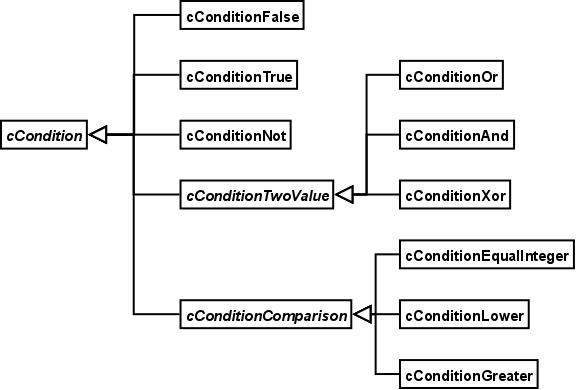
\includegraphics[scale=0.4]{fib_conditions}
\end{center}
\caption{Klassengraph der Bedingungen}
\label{figClassConditions}
\end{figure}


\bigskip\noindent
Es gibt vier Arten von Bedingungen:
\begin{itemize}
 \item Nullstellige (keine Eingabeparameter bzw. enthaltende Bedingungen)
 \item Einstellige (einen Eingabeparameter bzw. enthaltende Bedingungen)
 \item Zweistellige (zwei Eingabeparameter bzw. enthaltende Bedingungen)
 \item Vergleiche (arbeiten auf zwei Unterfunktionen, welche Werte/ Zahlen bereitstellen)
\end{itemize}

\bigskip\noindent
Die Klassen f"ur die nullstelligen Bedingungen realisieren Wahrheitswerte, diese sind:
\begin{itemize}
 \item \verb|cConditionFalse|: Diese Bedingung ist immer falsch/ Unwahr.
 \item \verb|cConditionTrue|: Diese Bedingung ist immer wahr.
\end{itemize}

\bigskip\noindent
Die Klasse f"ur die einstelligen Bedingung ist \verb|cConditionNot| . Sie realisiert die Negation einer Aussage.

\bigskip\noindent
Die Klassen, welche zweistelligen Bedingung darstellen, werden von der Basisklasse \verb|cConditionTwoValue| abgeleitet.

\bigskip\noindent
Zu diesen zweistelligen Bedingungen geh"oren:
\begin{itemize}
 \item \verb|cConditionOr|: Die ``Oder'' Verkn"upfung zweier Wahrheitswerte.
 \item \verb|cConditionAnd|: Die ``Und'' Verkn"upfung zweier Wahrheitswerte.
 \item \verb|cConditionXor|: Die ``Entweder oder'' Verkn"upfung zweier Wahrheitswerte.
\end{itemize}

\bigskip\noindent
Die Klassen, welche Vergleiche von Werten implementieren, werden von der Basisklasse \verb|cConditionComparison| abgeleitet.

\bigskip\noindent
Zu diesen Vergleichen geh"oren:
\begin{itemize}
 \item \verb|cConditionEqualInteger|: Pr"ufung auf Gleichheit, zweier auf Ganzzahlen gerundeter Werte.
 \item \verb|cConditionLower|: Pr"ufung, ob der erste Wert kleiner als der zweite ist.
 \item \verb|cConditionGreater|: Pr"ufung, ob der erste Wert gr"o"ser als der zweite ist.
\end{itemize}


\subsection{Schnittstellenbeschreibung}

\subsubsection{getValue}\index{cCondition!getValue()}\index{getValue()}

\textbf{Syntax:} \verb|bool getValue() const|

\bigskip\noindent
Diese Methode wertet die Bedingung aus. Dabei werden auch in der Bedingung enthaltenden Bedingung ausgewertet.

Wenn eine enthaltende Bedingung der Bedingung nicht existiert, wird f"ur sie der \verb|false| (=falsch) angenommen.

\bigskip\noindent
\textbf{Eingabeparameter:} keine

\bigskip\noindent
\textbf{R"uckgabe:} Der Wahrheitswert zu dem die Bedingung ausgewertet wurde.


\subsubsection{getType}\index{cCondition!getType()}\index{getType()}

\textbf{Syntax:} \verb|intFib getType() const|

\bigskip\noindent
Diese Methode gibt eine Ganzzahl zur"uck, "uber die der Typ der Bedingung bestimmt werden kann. F"ur diese Typen werden auch Konstanten in der Basisklasse \verb|cCondition| definiert.

\bigskip\noindent
\textbf{M"ogliche Typen sind:}

\noindent
\begin{tabular}{|p{10mm}|p{60mm}|p{40mm}|}\hline
	Typ\-zei\-chen & Bedingung & Konstante \\\hline\hline
	00 & \verb|cConditionFalse|: Diese Bedingung ist immer ist falsch/ Unwahr. & \verb|CONDITION_FALSE| \\\hline
	01 & \verb|cConditionTrue|: Diese Bedingung ist immer ist wahr. & \verb|CONDITION_TRUE| \\\hline
	10 & \verb|cConditionNot|: Diese Bedingung realisiert die Negation einer Aussage. & \verb|CONDITION_NOT| \\\hline
	20 & \verb|cConditionOr|: Die ``Oder'' Verkn"upfung zweier Wahrheitswerte. & \verb|CONDITION_OR| \\\hline
	21 & \verb|cConditionAnd|: Die ``Und'' Verkn"upfung zweier Wahrheitswerte. & \verb|CONDITION_AND| \\\hline
	22 & \verb|cConditionXor|: Die ``Entweder oder'' Verkn"upfung zweier Wahrheitswerte. & \verb|CONDITION_XOR| \\\hline
	30 & \verb|cConditionEqualInteger|: Pr"ufung auf Gleichheit, zweier auf Ganzzahlen gerundeter Werte. & \verb|CONDITION_EQUAL_| \verb|INTEGER| \\\hline
	31 & \verb|cConditionLower|: Pr"ufung, ob der erste Wert kleiner als der zweite ist. & \verb|CONDITION_LOWER| \\\hline
	32 & \verb|cConditionGreater|: Pr"ufung, ob der erste Wert gr"o"ser als der zweite ist. & \verb|CONDITION_GREATER| \\\hline
\end{tabular}

\bigskip\noindent
\textbf{Eingabeparameter:} keine

\bigskip\noindent
\textbf{R"uckgabe:} Eine Ganzzahl, "uber die der Typ der Bedingung bestimmt werden kann.


\subsubsection{isValid}\index{cCondition!isValid()}\index{isValid()}

\textbf{Syntax:} \verb|bool isValid() const|

\bigskip\noindent
Diese Methode pr"uft, ob die Bedingung korrekt ist.

Damit eine Bedingung korrekt ist, m"ussen alle direkt oder indirekt enthaltenden Bedingung korrekt sein.
Die in einer korrekten Bedingung enthaltende Vergleichen (von der Klasse \verb|cConditionComparison| abgeleitet Unterklassen) enthaltenden Elemente sind korrekte Unterfunktionen (dies wird mit der \verb|isValid()|-Methode der Unterfunktionen gepr"uft).
Eine korrekte Bedingung darf sich nicht selbst enthalten und keine direkt oder indirekt enthaltende Bedingung oder Unterfunktionen mehr als einmal enthalten. Das hei"st, die direkt oder indirekt enthaltenden Bedingung und Unterfunktionen haben die Struktur eines (zyklenfreien) Baums.

\bigskip\noindent
\textbf{Eingabeparameter:} keine

\bigskip\noindent
\textbf{R"uckgabe:} Wenn die Bedingung korrekt ist, wird \verb|true| (=wahr) zur"uckgegeben, sonst \verb|false| (=falsch).


\subsection{cConditionFalse}\index{cCondition!cConditionFalse}\index{cConditionFalse}\index{Bedingungen!Falsche}

Die Klasse \verb|cConditionFalse| stellt eine Bedingung dar, die immer falsch ist.

\subsubsection{cConditionFalse}

\textbf{Syntax:} \verb|cConditionFalse()|

\bigskip\noindent
Der Konstruktor der falschen Bedingung, er erstellt einen falschen Bedingung.

\bigskip\noindent
\textbf{Eingabeparameter:} keine

\bigskip\noindent
\textbf{R"uckgabe:} keine


\subsubsection{getValue}\index{cConditionFalse!getValue()}\index{getValue()}

\textbf{Syntax:} \verb|bool getValue() const|

\bigskip\noindent
Diese Methode gibt immer \verb|false| (=falsch) zur"uck.

\bigskip\noindent
\textbf{Eingabeparameter:} keine

\bigskip\noindent
\textbf{R"uckgabe:} Es wird immer \verb|false| (=falsch) zur"uckgegeben.


\subsection{cConditionTrue}\index{cCondition!cConditionTrue}\index{cConditionTrue}\index{Bedingungen!Wahre}

Die Klasse \verb|cConditionTrue| stellt eine Bedingung dar, die immer wahr ist.

\subsubsection{cConditionTrue}

\textbf{Syntax:} \verb|cConditionTrue()|

\bigskip\noindent
Der Konstruktor der wahre Bedingung, er erstellt einen wahre Bedingung.

\bigskip\noindent
\textbf{Eingabeparameter:} keine

\bigskip\noindent
\textbf{R"uckgabe:} keine


\subsubsection{getValue}\index{cConditionTrue!getValue()}\index{getValue()}

\textbf{Syntax:} \verb|bool getValue() const|

\bigskip\noindent
Diese Methode gibt immer \verb|true| (=wahr) zur"uck.

\bigskip\noindent
\textbf{Eingabeparameter:} keine

\bigskip\noindent
\textbf{R"uckgabe:} Es wird immer \verb|true| (=wahr) zur"uckgegeben.



\subsection{cConditionNot}\index{cCondition!cConditionNot}\index{cConditionNot}\index{Bedingungen!Negation}

Die Klasse \verb|cConditionNot| stellt eine Bedingung dar, welche den entgegengesetzten Wahrheitswert hat, wie die enthaltende Bedingung. Ist die enthaltende Bedingung wahr ist die \verb|cConditionNot| Bedingung falsch. Ist die enthaltende Bedingung falsch ist die \verb|cConditionNot| Bedingung wahr.

\subsubsection{cConditionNot}

\bigskip\noindent
\textbf{Syntax:} \verb|cConditionNot( cCondition * pSubCondition )|

\bigskip\noindent
Der Konstruktor der Negationsbedingung, er erstellt eine Negationsbedingung.

Von dem Objekt \verb|pSubCondition| wird dabei keine Kope erstellt.

\bigskip\noindent
\textbf{Eingabeparameter:}
\begin{itemize}
 \item \verb|pSubCondition|: Einen Zeiger auf die Bedingung, welche die Negationsbedingung enthalten soll.
\end{itemize}

\bigskip\noindent
\textbf{R"uckgabe:} keine


\subsubsection{getValue}\index{cConditionNot!getValue()}\index{getValue()}

\textbf{Syntax:} \verb|bool getValue() const|

\bigskip\noindent
Diese Methode gibt den Wahrheitswert zur"uck, der das Gegenteil des Wahrheitswerts der enthaltenden Bedingung (mit \verb|getValue()| dieser ermittelt) ist.

Ist die enthaltende Bedingung \verb|true| (=wahr), ist die \verb|cConditionNot| Bedingung \verb|false| (=falsch). Ist die enthaltende Bedingung \verb|false| (=falsch), ist die \verb|cConditionNot| Bedingung \verb|true| (=wahr).

\bigskip\noindent
\textbf{Eingabeparameter:} keine

\bigskip\noindent
\textbf{R"uckgabe:} Den Wahrheitswert, der das Gegenteil des Wahrheitswerts der enthaltenden Bedingung ist (mit \verb|getValue()| dieser ermittelt).


\subsubsection{getSubCondition}\index{cConditionNot!getSubCondition()}\index{getSubCondition()}

\textbf{Syntax:} \verb|cCondition * getSubCondition()|

\bigskip\noindent
Diese Methode gibt einen Zeiger auf die in der Negationsbedingung enthaltende Bedingung zur"uck.

Existiert keine enthaltende Bedingung, wird der Nullpointer \verb|NULL| zur"uckgegeben.

\bigskip\noindent
\textbf{Eingabeparameter:} keine

\bigskip\noindent
\textbf{R"uckgabe:} Einen Zeiger auf die in der Negationsbedingung enthaltende Bedingung oder der Nullpointer \verb|NULL| , wenn keine enthaltende Bedingung existiert.


\subsubsection{setSubCondition}\index{cConditionNot!setSubCondition()}\index{setSubCondition}

\textbf{Syntax:} \verb|bool setSubCondition( cCondition| \\\verb| * pSubCondition, bool bDeleteOld=true )|

\bigskip\noindent
Diese Methode setzt die in der Negationsbedingung enthaltende Bedingung auf \verb|pSubCondition|. Dabei wird keine Kopie von \verb|pSubCondition| erstellt.

\bigskip\noindent
\textbf{Eingabeparameter:}
\begin{itemize}
 \item \verb|pSubCondition|: Einen Zeiger auf die Bedingung, welche die Negationsbedingung enthalten soll.
 \item \verb|bDeleteOld|: Dieser Parameter gibt an, ob die alte enthaltende Bedingung gel"oscht werden soll. Wenn der Wert \verb|true| (=wahr) ist, wird die alte enthaltende Bedingung (aus dem Arbeitsspeicher) gel"oscht. Standardwert ist \verb|true|, um die alte enthaltende Bedingung zu l"oschen.
\end{itemize}

\bigskip\noindent
\textbf{R"uckgabe:} Wenn die entahltende Bedingung auf \verb|pSubCondition| gesetzt wurde \verb|true| (=wahr), sonst \verb|false| (=falsch)


\subsection{cConditionTwoValue}\index{cCondition!cConditionTwoValue}\index{cConditionTwoValue}\index{Bedingungen!Zweistellige}


Die Klasse \verb|cConditionTwoValue| ist die Basisklasse aller zweistelligen Bedingungen. Von der Klasse \verb|cConditionTwoValue| k"onnen keine Instanzen erzeugt werden.

Zweistellig Bedingungen enthalten zwei Bedingungen. Beim Ermitteln des Wahrheitswerts der Bedingungen mit \verb|getValue()| , werden zuerst die Wahrheitswerts der enthaltenden Bedingungen ermittelt (mit \verb|getValue()|), wobei der Wahrheitswerts der ersten enthaltenden Bedingungen zuerst ermittelt wird. Existiert eine enthaltenden Bedingungen nicht, wird der Wahrheitswert falsch (=\verb|false|) als Wert dieser enthaltenden Bedingungen angenommen. Bei der Berechnung des Wahrheitswerts der Bedingung, wird also f"ur fehlende Bedingungen der Wahrheitswert falsch (=\verb|false|) eingesetzt.

\bigskip\noindent
Zweistellige Bedingungen sind:
\begin{itemize}
 \item \verb|cConditionOr|: Die ``Oder'' Verkn"upfung zweier Wahrheitswerte.
 \item \verb|cConditionAnd|: Die ``Und'' Verkn"upfung zweier Wahrheitswerte.
 \item \verb|cConditionXor|: Die ``Entweder oder'' Verkn"upfung zweier Wahrheitswerte.
\end{itemize}

Im Folgenden werden zuerst die Methoden f"ur zweistellige Bedingungen vorgestellt und dann die Klassen der m"oglichen zweistellige Bedingungen.


\subsubsection{getFirstSubCondition}\index{cConditionTwoValue!getFirstSubCondition()}\index{getFirstSubCondition()}

\textbf{Syntax:} \verb|cCondition * getFirstSubCondition()|

\bigskip\noindent
Diese Methode gibt einen Zeiger auf die erste in der Bedingungen enthaltende Bedingung zur"uck.

Existiert keine erste enthaltende Bedingung, wird der Nullpointer \verb|NULL| zur"uckgegeben.

\bigskip\noindent
\textbf{Eingabeparameter:} keine

\bigskip\noindent
\textbf{R"uckgabe:} Einen Zeiger auf die erste in der Bedingungen enthaltende Bedingung oder der Nullpointer \verb|NULL| , wenn keine erste enthaltende Bedingung existiert.


\subsubsection{setFirstSubCondition}\index{cConditionTwoValue!setFirstSubCondition()}\index{setFirstSubCondition()}

\textbf{Syntax:} \verb|bool setFirstSubCondition(| \\\verb| cCondition * pSubCondition, bool bDeleteOld=true )|

\bigskip\noindent
Diese Methode setzt die erste in der Bedingungen enthaltende Bedingung auf die "ubergebende Unterbedingung \verb|pSubCondition|. Dabei wird keine Kopie von \verb|pSubCondition| erstellt.

\bigskip\noindent
\textbf{Eingabeparameter:}
\begin{itemize}
 \item \verb|pSubCondition|: Einen Zeiger auf die Bedingung, welche die erste Unternbedingungen enthalten soll.
 \item \verb|bDeleteOld|: Dieser Parameter gibt an, ob die alte erste enthaltende Bedingung gel"oscht werden soll. Wenn der Wert \verb|true| (=wahr) ist, wird die erste alte enthaltende Bedingung (aus dem Arbeitsspeicher) gel"oscht, sonst, wenn er \verb|false| (=falsch) ist, nicht. Standardwert ist \verb|true|, um die erste alte enthaltende Bedingung zu l"oschen.
\end{itemize}

\bigskip\noindent
\textbf{R"uckgabe:} Wenn die entahltende erste Bedingung auf \verb|pSubCondition| gesetzt wurde \verb|true| (=wahr), sonst \verb|false| (=falsch)


\subsubsection{getSecondSubCondition}\index{cConditionTwoValue!getSecondSubCondition()}\index{getSecondSubCondition()}

\textbf{Syntax:} \verb|cCondition * getSecondSubCondition()|

\bigskip\noindent
Diese Methode gibt einen Zeiger auf die zweite in der Bedingungen enthaltende Bedingung zur"uck.

Existiert keine zweite enthaltende Bedingung, wird der Nullpointer \verb|NULL| zur"uckgegeben.

\bigskip\noindent
\textbf{Eingabeparameter:} keine

\bigskip\noindent
\textbf{R"uckgabe:} Einen Zeiger auf die zweite in der Bedingungen enthaltende Bedingung oder der Nullpointer \verb|NULL| , wenn keine zweite enthaltende Bedingung existiert.


\subsubsection{setSecondSubCondition}\index{cConditionTwoValue!setSecondSubCondition()}\index{setSecondSubCondition()}

\textbf{Syntax:} \verb|bool setSecondSubCondition(| \\\verb| cCondition * pSubCondition, bool bDeleteOld=true )|

\bigskip\noindent
Diese Methode setzt die zweite in der Bedingungen enthaltende Bedingung auf \verb|pSubCondition|. Dabei wird keine Kopie von \verb|pSubCondition| erstellt.

\bigskip\noindent
\textbf{Eingabeparameter:}
\begin{itemize}
 \item \verb|pSubCondition|: Einen Zeiger auf die Bedingung, welche die zweite Unternbedingungen enthalten soll.
 \item \verb|bDeleteOld|: Dieser Parameter gibt an, ob die alte zweite enthaltende Bedingung gel"oscht werden soll. Wenn der Wert \verb|true| (=wahr) ist, wird die zweite alte enthaltende Bedingung (aus dem Arbeitsspeicher) gel"oscht, sonst, wenn er \verb|false| (=falsch) ist, nicht. Standardwert ist \verb|true|, um die zweite alte enthaltende Bedingung zu l"oschen.
\end{itemize}

\bigskip\noindent
\textbf{R"uckgabe:} Wenn die entahltende zweite Bedingung auf \verb|pSubCondition| gesetzt wurde \verb|true| (=wahr), sonst \verb|false| (=falsch)


\subsubsection{cConditionOr}\index{cCondition!cConditionOr}\index{cConditionOr}\index{Bedingungen!Oder}

Die Klasse \verb|cConditionOr| realisiert die ``Or''-Bedingung zweier Unterbedingungen. Die ``Or''-Bedingung ist wahr (=\verb|true|), wenn mindestens eine der Unterbedingungen wahr (=\verb|true|) ist, sonst ist sie falsch  (=\verb|false|).

\paragraph{cConditionOr}

\ \\\\\noindent
\textbf{Syntax:} \verb|cConditionOr( cCondition * pFirstSubCondition,| \\\verb| cCondition * pSecondSubCondition )|

\bigskip\noindent
Der Konstruktor der ``Or''-Bedingung, er erstellt eine ``Or''-Bedingung. Es wird keine Kopie von \verb|pFirstSubCondition| oder \verb|pSecondSubCondition| erstellt.

\bigskip\noindent
\textbf{Eingabeparameter:}
\begin{itemize}
 \item \verb|pFirstSubCondition|: Einen Zeiger auf die erste Unterbedingung, welche die ``Or''-Bedingung enthalten soll.
 \item \verb|pSecondSubCondition|: Einen Zeiger auf die zweite Unterbedingung, welche die ``Or''-Bedingung enthalten soll.
\end{itemize}

\bigskip\noindent
\textbf{R"uckgabe:} keine


\paragraph{getValue}\index{cConditionOr!getValue()}\index{getValue()}

\ \\\\\noindent
\textbf{Syntax:} \verb|bool getValue() const|

\bigskip\noindent
Diese Methode gibt \verb|true| (=wahr) zur"uck, wenn mindestens einer der Wahrheitswerte der enthaltenden Unterbedingungen (mit \verb|getValue()| dieser ermittelt) \verb|true| (=wahr) ist, sonst gibt sie \verb|false| (=falsch) zur"uck.

\bigskip\noindent
\textbf{Eingabeparameter:} keine

\bigskip\noindent
\textbf{R"uckgabe:} Es wird \verb|true| (=wahr) zur"uckgegeben, wenn mindestens einer der Wahrheitswerte der enthaltenden Unterbedingungen (mit \verb|getValue()| dieser ermittelt) \verb|true| (=wahr) ist, sonst \verb|false| (=falsch).


\subsubsection{cConditionAnd}\index{cCondition!cConditionAnd}\index{cConditionAnd}\index{Bedingungen!Und}

Die Klasse \verb|cConditionAnd| realisiert die ``And''-Bedingung zweier Unterbedingungen. Die ``And''-Bedingung ist wahr (=\verb|true|), wenn beide der Unterbedingungen wahr (=\verb|true|) sind, sonst ist sie falsch  (=\verb|false|).

\paragraph{cConditionAnd}

\ \\\\\noindent
\textbf{Syntax:} \verb|cConditionAnd( cCondition * pFirstSubCondition,| \\\verb| cCondition * pSecondSubCondition )|

\bigskip\noindent
Der Konstruktor der ``And''-Bedingung, er erstellt eine ``And''-Bedingung. Dabei wird keine Kopie von dem Objekt \verb|pFirstSubCondition| oder dem Objekt \verb|pSecondSubCondition| erstellt.

\bigskip\noindent
\textbf{Eingabeparameter:}
\begin{itemize}
 \item \verb|pFirstSubCondition|: Einen Zeiger auf die erste Unterbedingung, welche die ``And''-Bedingung enthalten soll.
 \item \verb|pSecondSubCondition|: Einen Zeiger auf die zweite Unterbedingung, welche die ``And''-Bedingung enthalten soll.
\end{itemize}

\bigskip\noindent
\textbf{R"uckgabe:} keine


\paragraph{getValue}\index{cConditionAnd!getValue()}\index{getValue()}

\ \\\\\noindent
\textbf{Syntax:} \verb|bool getValue() const|

\bigskip\noindent
Diese Methode gibt \verb|true| (=wahr) zur"uck, wenn beide der Wahrheitswerte der enthaltenden Unterbedingungen (mit \verb|getValue()| dieser ermittelt) \verb|true| (=wahr) sind, sonst gibt sie \verb|false| (=falsch) zur"uck.

\bigskip\noindent
\textbf{Eingabeparameter:} keine

\bigskip\noindent
\textbf{R"uckgabe:} Es wird \verb|true| (=wahr) zur"uckgegeben, wenn beide der Wahrheitswerte der enthaltenden Unterbedingungen (mit \verb|getValue()| dieser ermittelt) \verb|true| (=wahr) sind, sonst \verb|false| (=falsch).


\subsubsection{cConditionXor}\index{cCondition!cConditionXor}\index{cConditionXor}\index{Bedingungen!Xor}

Die Klasse \verb|cConditionXor| realisiert die ``Xor''-Bedingung zweier Unterbedingungen. Die ``Xor''-Bedingung ist wahr (=\verb|true|), wenn genau eine der Unterbedingungen wahr (=\verb|true|) ist, sonst ist sie falsch  (=\verb|false|).

\paragraph{cConditionXor}

\ \\\\\noindent
\textbf{Syntax:} \verb|cConditionXor( cCondition * pFirstSubCondition,| \\\verb| cCondition * pSecondSubCondition )|

\bigskip\noindent
Der Konstruktor der ``Xor''-Bedingung, er erstellt eine ``Xor''-Bedingung. Dabei wird keine Kopie von dem Objekt \verb|pFirstSubCondition| oder dem Objekt \verb|pSecondSubCondition| erstellt.

\bigskip\noindent
\textbf{Eingabeparameter:}
\begin{itemize}
 \item \verb|pFirstSubCondition|: Einen Zeiger auf die erste Unterbedingung, welche die ``Xor''-Bedingung enthalten soll.
 \item \verb|pSecondSubCondition|: Einen Zeiger auf die zweite Unterbedingung, welche die ``Xor''-Bedingung enthalten soll.
\end{itemize}

\bigskip\noindent
\textbf{R"uckgabe:} keine


\paragraph{getValue}\index{cConditionXor!getValue()}\index{getValue()}

\ \\\\\noindent
\textbf{Syntax:} \verb|bool getValue() const|

\bigskip\noindent
Diese Methode gibt \verb|true| (=wahr) zur"uck, wenn genau einer der Wahrheitswerte der enthaltenden Unterbedingungen (mit \verb|getValue()| dieser ermittelt) \verb|true| (=wahr) ist, sonst gibt sie \verb|false| (=falsch) zur"uck.

\bigskip\noindent
\textbf{Eingabeparameter:} keine

\bigskip\noindent
\textbf{R"uckgabe:} Es wird \verb|true| (=wahr) zur"uckgegeben, wenn genau einer der Wahrheitswerte der enthaltenden Unterbedingungen (mit \verb|getValue()| dieser ermittelt) \verb|true| (=wahr) ist, sonst \verb|false| (=falsch).



\subsection{cConditionComparison}\index{cCondition!cConditionComparison}\index{cConditionComparison}\index{Bedingungen!Vergleiche}


Die Klasse \verb|cConditionComparison| ist die Basisklasse aller Vergleiche. Von der Klasse \verb|cConditionComparison| k"onnen keine Instanzen erzeugt werden.

Vergleiche geschehen immer auf zwei Unterfunktionen.

Vergleiche enthalten zwei Unterfunktionen. Beim Ermitteln des Wahrheitswerts des Vergleichs mit \verb|getValue()| , werden zuerst die Werte der enthaltenden Unterfunktionen ermittelt (mit \verb|getValue()|), wobei der Wert der ersten enthaltenden Unterfunktion zuerst ermittelt wird. Existiert eine enthaltenden Unterfunktion nicht, wird der Nullwert des Definitionsbereichs f"ur Unterfunktionen als Wert dieser Unterfunktion angenommen. Bei der Berechnung des Wahrheitswerts, wird also f"ur fehlende Unterfunktionen der Nullwert eingesetzt.

\bigskip\noindent
Vergleiche sind:
\begin{itemize}
 \item \verb|cConditionEqualInteger|: Pr"ufung auf Gleichheit, zweier auf Ganzzahlen gerundeter Werte.
 \item \verb|cConditionLower|: Pr"ufung, ob der erste Wert kleiner als der zweite ist.
 \item \verb|cConditionGreater|: Pr"ufung, ob der erste Wert gr"o"ser als der zweite ist.
\end{itemize}

Im Folgenden werden zuerst die Methoden f"ur Vergleiche vorgestellt und dann die Klassen der m"oglichen Vergleiche.



\subsubsection{getFirstUnderFunction}\index{cConditionComparison!getFirstUnderFunction()}\index{getFirstUnderFunction()}

\textbf{Syntax:} \verb|cUnderFunction * getFirstUnderFunction()|

\bigskip\noindent
Diese Methode gibt einen Zeiger auf die erste in dem Vergleich enthaltende Unterfunktion zur"uck.

Existiert keine erste enthaltende Unterfunktion, wird der Nullpointer \verb|NULL| zur"uckgegeben.

\bigskip\noindent
\textbf{Eingabeparameter:} keine

\bigskip\noindent
\textbf{R"uckgabe:} Einen Zeiger auf die erste in dem Vergleich enthaltende Unterfunktion oder der Nullpointer \verb|NULL| , wenn keine erste enthaltende Unterfunktion existiert.


\subsubsection{setFirstUnderFunction}\index{cConditionComparison!setFirstUnderFunction()}\index{setFirstUnderFunction()}

\textbf{Syntax:} \verb|void setFirstUnderFunction(| \\\verb| cUnderFunction *pUnderFunction, bool bDeleteOld=true )|

\bigskip\noindent
Diese Methode setzt die erste in dem Vergleich enthaltende Unterfunktion auf \verb|pUnderFunction|. Dabei wird keine Kopie von \verb|pUnderFunction| erstellt.

\bigskip\noindent
\textbf{Eingabeparameter:}
\begin{itemize}
 \item \verb|pUnderFunction|: Einen Zeiger auf die Unterfunktion, welche als die erste Unterfunktion enthalten sein soll.
 \item \verb|bDeleteOld|: Dieser Parameter gibt an, ob die erste alte enthaltende Unterfunktion gel"oscht werden soll. Wenn der Wert \verb|true| (=wahr) ist, wird die erste alte enthaltende Unterfunktion (aus dem Arbeitsspeicher) gel"oscht, sonst, wenn der Wert \verb|false| (=falsch) ist, nicht. Standardwert ist \verb|true|, um die erste alte enthaltende Unterfunktion zu l"oschen.
\end{itemize}

\bigskip\noindent
\textbf{R"uckgabe:} keine


\subsubsection{getSecondUnderFunction}\index{cConditionComparison!getSecondUnderFunction()}\index{getSecondUnderFunction()}

\textbf{Syntax:} \verb|cUnderFunction * getSecondUnderFunction()|

\bigskip\noindent
Diese Methode gibt einen Zeiger auf die zweite in dem Vergleich enthaltende Unterfunktion zur"uck.

Existiert keine zweite enthaltende Unterfunktion, wird der Nullpointer \verb|NULL| zur"uckgegeben.

\bigskip\noindent
\textbf{Eingabeparameter:} keine

\bigskip\noindent
\textbf{R"uckgabe:} Einen Zeiger auf die zweite in dem Vergleich enthaltende Unterfunktion oder der Nullpointer \verb|NULL| , wenn keine zweite enthaltende Unterfunktion existiert.


\subsubsection{setSecondUnderFunction}\index{cConditionComparison!setSecondUnderFunction()}\index{setSecondUnderFunction()}

\textbf{Syntax:} \verb|void setSecondUnderFunction(| \\\verb| cUnderFunction *pUnderFunction, bool bDeleteOld=true )|

\bigskip\noindent
Diese Methode setzt die zweite in dem Vergleich enthaltende Unterfunktion auf \verb|pUnderFunction|. Dabei wird keine Kopie von \verb|pUnderFunction| erstellt.

\bigskip\noindent
\textbf{Eingabeparameter:}
\begin{itemize}
 \item \verb|pUnderFunction|: Einen Zeiger auf die Unterfunktion, welche als die zweite Unterfunktion enthalten sein soll.
 \item \verb|bDeleteOld|: Dieser Parameter gibt an, ob die alte zweite enthaltende Unterfunktion gel"oscht werden soll. Wenn der Wert \verb|true| (=wahr) ist wird die zweite alte enthaltende Unterfunktion (aus dem Arbeitsspeicher) gel"oscht, sonst, wenn der Wert \verb|false| (=falsch) ist, nicht. Standardwert ist \verb|true|, um die zweite alte enthaltende Unterfunktion zu l"oschen.
\end{itemize}

\bigskip\noindent
\textbf{R"uckgabe:} keine


\subsubsection{cConditionEqualInteger}\index{cConditionComparison!cConditionEqualInteger}\index{cConditionEqualInteger}\index{Bedingungen!Gleichheit von Ganzzahlen}

Die Klasse \verb|cConditionEqualInteger| realisiert den Vergleich auf Gleichheit der auf Ganzahlen gerundeten Werte zweier Unterfunktionen. Der Vergleich \verb|cConditionEqualInteger| ist wahr (=\verb|true|), wenn die Werte beider Unterfunktionen auf Ganzzahlen gerundet gleich sind, sonst ist sie falsch  (=\verb|false|).

Wenn die Werte der Unterfunktionen gerundet werden, wird ihr Wert auf die Ganzzahl gerundet, die ihm am n"achsten ist (=kleinster Abstand). Gibt es mehrere n"achste Ganzzahlen, so wird die kleinste zum Vergleich genommen (bei $0,5$ wird immer abgerundet). Nach M"oglichkeit sollten die Werte der Unterfunktionen aber schon Ganzzahlen entsprechen, so dass es nicht zu Rundungsfehlern kommen kann.


\paragraph{cConditionEqualInteger}

\ \\\\\noindent
\textbf{Syntax:} \verb|cConditionEqualInteger(| \\\verb| cUnderFunction * pFirstUnderFunction,| \\\verb| cUnderFunction * pSecondUnderFunction )|

\bigskip\noindent
Der Konstruktor des Vergleichs auf Gleichheit, er erstellt eine Vergleich auf Gleichheit. Dabei wird keine Kopie von dem Objekt \verb|pFirstUnderFunction| oder dem Objekt \verb|pSecondUnderFunction| erstellt.

\bigskip\noindent
\textbf{Eingabeparameter:}
\begin{itemize}
 \item \verb|pFirstUnderFunction|: Einen Zeiger auf die erste Unterfunktion, welche im Vergleich auf Gleichheit enthalten sein soll.
 \item \verb|pSecondUnderFunction|: Einen Zeiger auf die zweite Unterfunktion, welche im Vergleich auf Gleichheit enthalten sein soll.
\end{itemize}

\bigskip\noindent
\textbf{R"uckgabe:} keine


\paragraph{getValue}\index{cConditionEqualInteger!getValue()}\index{getValue()}

\ \\\\\noindent
\textbf{Syntax:} \verb|doubleFib getValue() const|

\bigskip\noindent
Diese Methode gibt \verb|true| (=wahr) zur"uck, wenn die Werte beider Unterfunktionen (mit \verb|getValue()| dieser ermittelt) auf Ganzzahlen gerundet gleich sind, sonst gibt sie \verb|false| (=falsch) zur"uck.

\bigskip\noindent
\textbf{Eingabeparameter:} keine

\bigskip\noindent
\textbf{R"uckgabe:} Es wird \verb|true| (=wahr) zur"uckgegeben, wenn die Werte beider Unterfunktionen (mit \verb|getValue()| dieser ermittelt) auf Ganzzahlen gerundet gleich sind, sonst gibt die Methode \verb|false| (=falsch) zur"uck.


\subsubsection{cConditionLower}\index{cConditionComparison!cConditionLower}\index{cConditionLower}\index{Bedingungen!Kleiner}

Die Klasse \verb|cConditionLower| realisiert den Vergleich auf Kleiner der Werte zweier Unterfunktionen. Der Vergleich \verb|cConditionLower| ist wahr (=\verb|true|), wenn die Werte der ersten Unterfunktionen kleiner als der Wert der zweiten Unterfunktionen ist, sonst ist sie falsch  (=\verb|false|).


\paragraph{cConditionLower}

\ \\\\\noindent
\textbf{Syntax:} \verb|cConditionLower(| \\\verb| cUnderFunction * pFirstUnderFunction,| \\\verb| cUnderFunction * pSecondUnderFunction )|

\bigskip\noindent
Der Konstruktor des Vergleichs auf kleiner, er erstellt eine Vergleich auf kleiner. Dabei wird keine Kopie von  dem Objekt \verb|pFirstUnderFunction| oder dem Objekt \verb|pSecondUnderFunction| erstellt.

\bigskip\noindent
\textbf{Eingabeparameter:}
\begin{itemize}
 \item \verb|pFirstUnderFunction|: Einen Zeiger auf die erste Unterfunktion, welche im Vergleich auf kleiner enthalten sein soll.
 \item \verb|pSecondUnderFunction|: Einen Zeiger auf die zweite Unterfunktion, welche im Vergleich auf kleiner enthalten sein soll.
\end{itemize}

\bigskip\noindent
\textbf{R"uckgabe:} keine


\paragraph{getValue}\index{cConditionLower!getValue()}\index{getValue()}

\ \\\\\noindent
\textbf{Syntax:} \verb|doubleFib getValue() const|

\bigskip\noindent
Diese Methode gibt \verb|true| (=wahr) zur"uck, wenn die Werte der ersten Unterfunktionen (mit \verb|getValue()| dieser ermittelt) kleiner als der Wert der zweiten Unterfunktionen (mit \verb|getValue()| dieser ermittelt) ist, sonst gibt sie \verb|false| (=falsch) zur"uck.

\bigskip\noindent
\textbf{Eingabeparameter:} keine

\bigskip\noindent
\textbf{R"uckgabe:} Es wird \verb|true| (=wahr) zur"uckgegeben, wenn die Werte der ersten Unterfunktionen (mit \verb|getValue()| dieser ermittelt) kleiner als der Wert der zweiten Unterfunktionen (mit \verb|getValue()| dieser ermittelt) ist, sonst gibt die Methode \verb|false| (=falsch) zur"uck.


\subsubsection{cConditionGreater}\index{cConditionComparison!cConditionGreater}\index{cConditionGreater}\index{Bedingungen!Greosser}

Die Klasse \verb|cConditionGreater| realisiert den Vergleich auf Gr"o"ser der Werte zweier Unterfunktionen. Der Vergleich \verb|cConditionGreater| ist wahr (=\verb|true|), wenn die Werte der ersten Unterfunktionen gr"o"ser als der Wert der zweiten Unterfunktionen ist, sonst ist sie falsch  (=\verb|false|).


\paragraph{cConditionGreater}

\ \\\\\noindent
\textbf{Syntax:} \verb|cConditionGreater(| \\\verb| cUnderFunction * pFirstUnderFunction,| \\\verb| cUnderFunction * pSecondUnderFunction )|

\bigskip\noindent
Der Konstruktor des Vergleichs auf gr"o"ser, er erstellt eine Vergleich auf gr"o"ser. Dabei wird keine Kopie von dem Objekt \verb|pFirstUnderFunction| oder dem Objekt \verb|pSecondUnderFunction| erstellt.

\bigskip\noindent
\textbf{Eingabeparameter:}
\begin{itemize}
 \item \verb|pFirstUnderFunction|: Einen Zeiger auf die erste Unterfunktion, welche im Vergleich auf gr"o"ser enthalten sein soll.
 \item \verb|pSecondUnderFunction|: Einen Zeiger auf die zweite Unterfunktion, welche im Vergleich auf gr"o"ser enthalten sein soll.
\end{itemize}

\bigskip\noindent
\textbf{R"uckgabe:} keine


\paragraph{getValue}\index{cConditionGreater!getValue()}\index{getValue()}

\ \\\\\noindent
\textbf{Syntax:} \verb|doubleFib getValue() const|

\bigskip\noindent
Diese Methode gibt \verb|true| (=wahr) zur"uck, wenn die Werte der ersten Unterfunktionen (mit \verb|getValue()| dieser ermittelt) gr"o"ser als der Wert der zweiten Unterfunktionen (mit \verb|getValue()| dieser ermittelt) ist, sonst gibt sie \verb|false| (=falsch) zur"uck.

\bigskip\noindent
\textbf{Eingabeparameter:} keine

\bigskip\noindent
\textbf{R"uckgabe:} Es wird \verb|true| (=wahr) zur"uckgegeben, wenn die Werte der ersten Unterfunktionen (mit \verb|getValue()| dieser ermittelt) gr"o"ser als der Wert der zweiten Unterfunktionen (mit \verb|getValue()| dieser ermittelt) ist, sonst gibt die Methode \verb|false| (=falsch) zur"uck.
























